% Options for packages loaded elsewhere
% Options for packages loaded elsewhere
\PassOptionsToPackage{unicode}{hyperref}
\PassOptionsToPackage{hyphens}{url}
\PassOptionsToPackage{dvipsnames,svgnames,x11names}{xcolor}
%
\documentclass[
  a4paper,
  DIV=11,
  numbers=noendperiod]{scrreprt}
\usepackage{xcolor}
\usepackage[top=2.5cm,bottom=2.5cm,left=2.5cm,right=2.5cm]{geometry}
\usepackage{amsmath,amssymb}
\setcounter{secnumdepth}{3}
\usepackage{iftex}
\ifPDFTeX
  \usepackage[T1]{fontenc}
  \usepackage[utf8]{inputenc}
  \usepackage{textcomp} % provide euro and other symbols
\else % if luatex or xetex
  \usepackage{unicode-math} % this also loads fontspec
  \defaultfontfeatures{Scale=MatchLowercase}
  \defaultfontfeatures[\rmfamily]{Ligatures=TeX,Scale=1}
\fi
\usepackage{lmodern}
\ifPDFTeX\else
  % xetex/luatex font selection
\fi
% Use upquote if available, for straight quotes in verbatim environments
\IfFileExists{upquote.sty}{\usepackage{upquote}}{}
\IfFileExists{microtype.sty}{% use microtype if available
  \usepackage[]{microtype}
  \UseMicrotypeSet[protrusion]{basicmath} % disable protrusion for tt fonts
}{}
\makeatletter
\@ifundefined{KOMAClassName}{% if non-KOMA class
  \IfFileExists{parskip.sty}{%
    \usepackage{parskip}
  }{% else
    \setlength{\parindent}{0pt}
    \setlength{\parskip}{6pt plus 2pt minus 1pt}}
}{% if KOMA class
  \KOMAoptions{parskip=half}}
\makeatother
% Make \paragraph and \subparagraph free-standing
\makeatletter
\ifx\paragraph\undefined\else
  \let\oldparagraph\paragraph
  \renewcommand{\paragraph}{
    \@ifstar
      \xxxParagraphStar
      \xxxParagraphNoStar
  }
  \newcommand{\xxxParagraphStar}[1]{\oldparagraph*{#1}\mbox{}}
  \newcommand{\xxxParagraphNoStar}[1]{\oldparagraph{#1}\mbox{}}
\fi
\ifx\subparagraph\undefined\else
  \let\oldsubparagraph\subparagraph
  \renewcommand{\subparagraph}{
    \@ifstar
      \xxxSubParagraphStar
      \xxxSubParagraphNoStar
  }
  \newcommand{\xxxSubParagraphStar}[1]{\oldsubparagraph*{#1}\mbox{}}
  \newcommand{\xxxSubParagraphNoStar}[1]{\oldsubparagraph{#1}\mbox{}}
\fi
\makeatother

\usepackage{color}
\usepackage{fancyvrb}
\newcommand{\VerbBar}{|}
\newcommand{\VERB}{\Verb[commandchars=\\\{\}]}
\DefineVerbatimEnvironment{Highlighting}{Verbatim}{commandchars=\\\{\}}
% Add ',fontsize=\small' for more characters per line
\usepackage{framed}
\definecolor{shadecolor}{RGB}{248,248,248}
\newenvironment{Shaded}{\begin{snugshade}}{\end{snugshade}}
\newcommand{\AlertTok}[1]{\textcolor[rgb]{0.94,0.16,0.16}{#1}}
\newcommand{\AnnotationTok}[1]{\textcolor[rgb]{0.56,0.35,0.01}{\textbf{\textit{#1}}}}
\newcommand{\AttributeTok}[1]{\textcolor[rgb]{0.13,0.29,0.53}{#1}}
\newcommand{\BaseNTok}[1]{\textcolor[rgb]{0.00,0.00,0.81}{#1}}
\newcommand{\BuiltInTok}[1]{#1}
\newcommand{\CharTok}[1]{\textcolor[rgb]{0.31,0.60,0.02}{#1}}
\newcommand{\CommentTok}[1]{\textcolor[rgb]{0.56,0.35,0.01}{\textit{#1}}}
\newcommand{\CommentVarTok}[1]{\textcolor[rgb]{0.56,0.35,0.01}{\textbf{\textit{#1}}}}
\newcommand{\ConstantTok}[1]{\textcolor[rgb]{0.56,0.35,0.01}{#1}}
\newcommand{\ControlFlowTok}[1]{\textcolor[rgb]{0.13,0.29,0.53}{\textbf{#1}}}
\newcommand{\DataTypeTok}[1]{\textcolor[rgb]{0.13,0.29,0.53}{#1}}
\newcommand{\DecValTok}[1]{\textcolor[rgb]{0.00,0.00,0.81}{#1}}
\newcommand{\DocumentationTok}[1]{\textcolor[rgb]{0.56,0.35,0.01}{\textbf{\textit{#1}}}}
\newcommand{\ErrorTok}[1]{\textcolor[rgb]{0.64,0.00,0.00}{\textbf{#1}}}
\newcommand{\ExtensionTok}[1]{#1}
\newcommand{\FloatTok}[1]{\textcolor[rgb]{0.00,0.00,0.81}{#1}}
\newcommand{\FunctionTok}[1]{\textcolor[rgb]{0.13,0.29,0.53}{\textbf{#1}}}
\newcommand{\ImportTok}[1]{#1}
\newcommand{\InformationTok}[1]{\textcolor[rgb]{0.56,0.35,0.01}{\textbf{\textit{#1}}}}
\newcommand{\KeywordTok}[1]{\textcolor[rgb]{0.13,0.29,0.53}{\textbf{#1}}}
\newcommand{\NormalTok}[1]{#1}
\newcommand{\OperatorTok}[1]{\textcolor[rgb]{0.81,0.36,0.00}{\textbf{#1}}}
\newcommand{\OtherTok}[1]{\textcolor[rgb]{0.56,0.35,0.01}{#1}}
\newcommand{\PreprocessorTok}[1]{\textcolor[rgb]{0.56,0.35,0.01}{\textit{#1}}}
\newcommand{\RegionMarkerTok}[1]{#1}
\newcommand{\SpecialCharTok}[1]{\textcolor[rgb]{0.81,0.36,0.00}{\textbf{#1}}}
\newcommand{\SpecialStringTok}[1]{\textcolor[rgb]{0.31,0.60,0.02}{#1}}
\newcommand{\StringTok}[1]{\textcolor[rgb]{0.31,0.60,0.02}{#1}}
\newcommand{\VariableTok}[1]{\textcolor[rgb]{0.00,0.00,0.00}{#1}}
\newcommand{\VerbatimStringTok}[1]{\textcolor[rgb]{0.31,0.60,0.02}{#1}}
\newcommand{\WarningTok}[1]{\textcolor[rgb]{0.56,0.35,0.01}{\textbf{\textit{#1}}}}

\usepackage{longtable,booktabs,array}
\usepackage{calc} % for calculating minipage widths
% Correct order of tables after \paragraph or \subparagraph
\usepackage{etoolbox}
\makeatletter
\patchcmd\longtable{\par}{\if@noskipsec\mbox{}\fi\par}{}{}
\makeatother
% Allow footnotes in longtable head/foot
\IfFileExists{footnotehyper.sty}{\usepackage{footnotehyper}}{\usepackage{footnote}}
\makesavenoteenv{longtable}
\usepackage{graphicx}
\makeatletter
\newsavebox\pandoc@box
\newcommand*\pandocbounded[1]{% scales image to fit in text height/width
  \sbox\pandoc@box{#1}%
  \Gscale@div\@tempa{\textheight}{\dimexpr\ht\pandoc@box+\dp\pandoc@box\relax}%
  \Gscale@div\@tempb{\linewidth}{\wd\pandoc@box}%
  \ifdim\@tempb\p@<\@tempa\p@\let\@tempa\@tempb\fi% select the smaller of both
  \ifdim\@tempa\p@<\p@\scalebox{\@tempa}{\usebox\pandoc@box}%
  \else\usebox{\pandoc@box}%
  \fi%
}
% Set default figure placement to htbp
\def\fps@figure{htbp}
\makeatother





\setlength{\emergencystretch}{3em} % prevent overfull lines

\providecommand{\tightlist}{%
  \setlength{\itemsep}{0pt}\setlength{\parskip}{0pt}}



 


% ------------------------------------------------------------------
% frontespizio.tex -- front page e retro della dispensa
% Incluso nello YAML con: include-in-header: frontespizio.tex
% Ridefinisce \maketitle (chiamato in automatico da Quarto)
% ------------------------------------------------------------------
\providecolor{blu}{rgb}{0.0,0.33,0.71}

\renewcommand{\maketitle}{%
  \begin{titlepage}
    \centering
    % --- Intestazione: ateneo, dipartimento, corso di laurea ---
    {\large\scshape Università degli Studi di Trento\par}
    \vspace{2mm}
    {\normalsize Dipartimento di Psicologia e Scienze Cognitive\par}
    \vspace{1mm}
    {\normalsize Corso di Laurea in Scienze e Tecniche di Psicologia Cognitiva\par}
    \vspace{6mm}
    {\color{blu}\rule{\textwidth}{0.8pt}\par}

    \vfill

    % --- Corso e titolo ---
    {\large Corso di\par}
    \vspace{2mm}
    {\LARGE\itshape Analisi dei dati con applicazioni informatiche\par}
    \vspace{18mm}
    {\color{blu}\fontsize{34}{40}\selectfont\bfseries Statistica descrittiva\par}
    \vspace{6mm}
    {\Large Dispensa -- Moduli 1, 2 e 3\par}

    \vfill

    % --- Autrice ---
    {\color{blu}\rule{\textwidth}{0.8pt}\par}
    \vspace{6mm}
    {\large Ottavia M. Epifania\par}
    \vspace{1mm}
    {\small\ttfamily ottavia.epifania@unitn.it\par}
  \end{titlepage}

  % --- Retro del frontespizio: disclaimer e licenza ---
  \thispagestyle{empty}
  \null\vfill
  \begin{small}
  \noindent\textbf{Nota sul materiale}\par
  \vspace{2mm}
  \noindent Parte del materiale di questa dispensa è riadattato dal corso
  \emph{Test per le organizzazioni} dell'Università degli Studi di Padova,
  tenuto insieme alla Dott.ssa Margherita Calderan
  (\url{https://ottaviae.github.io/test-organizzioni-fisppa/}).

  \vspace{8mm}
  \noindent\textbf{Licenza}\par
  \vspace{2mm}
  \noindent Quest'opera è distribuita con licenza
  \href{https://creativecommons.org/licenses/by/4.0/deed.it}{Creative Commons
  Attribuzione 4.0 Internazionale (CC BY 4.0)}.
  Puoi copiare, ridistribuire e modificare il materiale con qualsiasi mezzo
  e per qualsiasi fine, a condizione di citare l'autrice e di indicare se
  sono state apportate modifiche.

  \vspace{3mm}
  \noindent Per citare questa dispensa:\\
  Epifania, O. M. \emph{Statistica descrittiva. Dispensa del corso Analisi dei
  dati con applicazioni informatiche, Moduli 1, 2 e 3}. Università degli Studi
  di Trento.
  \end{small}
  \clearpage
}
\usepackage{booktabs}
\usepackage{longtable}
\usepackage{array}
\usepackage{multirow}
\usepackage{wrapfig}
\usepackage{float}
\usepackage{colortbl}
\usepackage{pdflscape}
\usepackage{tabu}
\usepackage{threeparttable}
\usepackage{threeparttablex}
\usepackage[normalem]{ulem}
\usepackage{makecell}
\usepackage{xcolor}
\KOMAoption{captions}{tableheading}
\usepackage{tikz}
\usepackage{multirow}
\usepackage{multicol}
\newcommand{\cov}{\mathrm{Cov}}
\usetikzlibrary{positioning,shapes,calc,arrows,decorations.pathreplacing,arrows.meta}
\definecolor{unipd}{RGB}{155,0,20}
\definecolor{template}{RGB}{72,79,89}
\definecolor{blu}{rgb}{0.0,0.33,0.71}
\makeatletter
\@ifpackageloaded{tcolorbox}{}{\usepackage[skins,breakable]{tcolorbox}}
\@ifpackageloaded{fontawesome5}{}{\usepackage{fontawesome5}}
\definecolor{quarto-callout-color}{HTML}{909090}
\definecolor{quarto-callout-note-color}{HTML}{0758E5}
\definecolor{quarto-callout-important-color}{HTML}{CC1914}
\definecolor{quarto-callout-warning-color}{HTML}{EB9113}
\definecolor{quarto-callout-tip-color}{HTML}{00A047}
\definecolor{quarto-callout-caution-color}{HTML}{FC5300}
\definecolor{quarto-callout-color-frame}{HTML}{acacac}
\definecolor{quarto-callout-note-color-frame}{HTML}{4582ec}
\definecolor{quarto-callout-important-color-frame}{HTML}{d9534f}
\definecolor{quarto-callout-warning-color-frame}{HTML}{f0ad4e}
\definecolor{quarto-callout-tip-color-frame}{HTML}{02b875}
\definecolor{quarto-callout-caution-color-frame}{HTML}{fd7e14}
\makeatother
\makeatletter
\@ifpackageloaded{caption}{}{\usepackage{caption}}
\AtBeginDocument{%
\ifdefined\contentsname
  \renewcommand*\contentsname{Table of contents}
\else
  \newcommand\contentsname{Table of contents}
\fi
\ifdefined\listfigurename
  \renewcommand*\listfigurename{List of Figures}
\else
  \newcommand\listfigurename{List of Figures}
\fi
\ifdefined\listtablename
  \renewcommand*\listtablename{List of Tables}
\else
  \newcommand\listtablename{List of Tables}
\fi
\ifdefined\figurename
  \renewcommand*\figurename{Figure}
\else
  \newcommand\figurename{Figure}
\fi
\ifdefined\tablename
  \renewcommand*\tablename{Table}
\else
  \newcommand\tablename{Table}
\fi
}
\@ifpackageloaded{float}{}{\usepackage{float}}
\floatstyle{ruled}
\@ifundefined{c@chapter}{\newfloat{codelisting}{h}{lop}}{\newfloat{codelisting}{h}{lop}[chapter]}
\floatname{codelisting}{Listing}
\newcommand*\listoflistings{\listof{codelisting}{List of Listings}}
\makeatother
\makeatletter
\makeatother
\makeatletter
\@ifpackageloaded{caption}{}{\usepackage{caption}}
\@ifpackageloaded{subcaption}{}{\usepackage{subcaption}}
\makeatother
\makeatletter
\@ifpackageloaded{tikz}{}{\usepackage{tikz}}
\makeatother
        \newcommand*\circled[1]{\tikz[baseline=(char.base)]{
          \node[shape=circle,draw,inner sep=1pt] (char) {{\scriptsize#1}};}}  
                  
\usepackage{bookmark}
\IfFileExists{xurl.sty}{\usepackage{xurl}}{} % add URL line breaks if available
\urlstyle{same}
\hypersetup{
  pdftitle={Statistica descrittiva},
  pdfauthor={Ottavia M. Epifania},
  colorlinks=true,
  linkcolor={blue},
  filecolor={Maroon},
  citecolor={Blue},
  urlcolor={Blue},
  pdfcreator={LaTeX via pandoc}}


\title{Statistica descrittiva}
\usepackage{etoolbox}
\makeatletter
\providecommand{\subtitle}[1]{% add subtitle to \maketitle
  \apptocmd{\@title}{\par {\large #1 \par}}{}{}
}
\makeatother
\subtitle{Dispensa del corso \emph{Analisi dei dati con applicazioni
informatiche} -- Moduli 1, 2 e 3}
\author{Ottavia M. Epifania}
\date{}
\begin{document}
\maketitle

\renewcommand*\contentsname{Indice}
{
\hypersetup{linkcolor=}
\setcounter{tocdepth}{1}
\tableofcontents
}

\chapter{\texorpdfstring{Modulo 1 -- Introduzione a
\texttt{R}}{Modulo 1 -- Introduzione a R}}\label{modulo-1-introduzione-a-r}

\section{RStudio}\label{rstudio}

\begin{center}
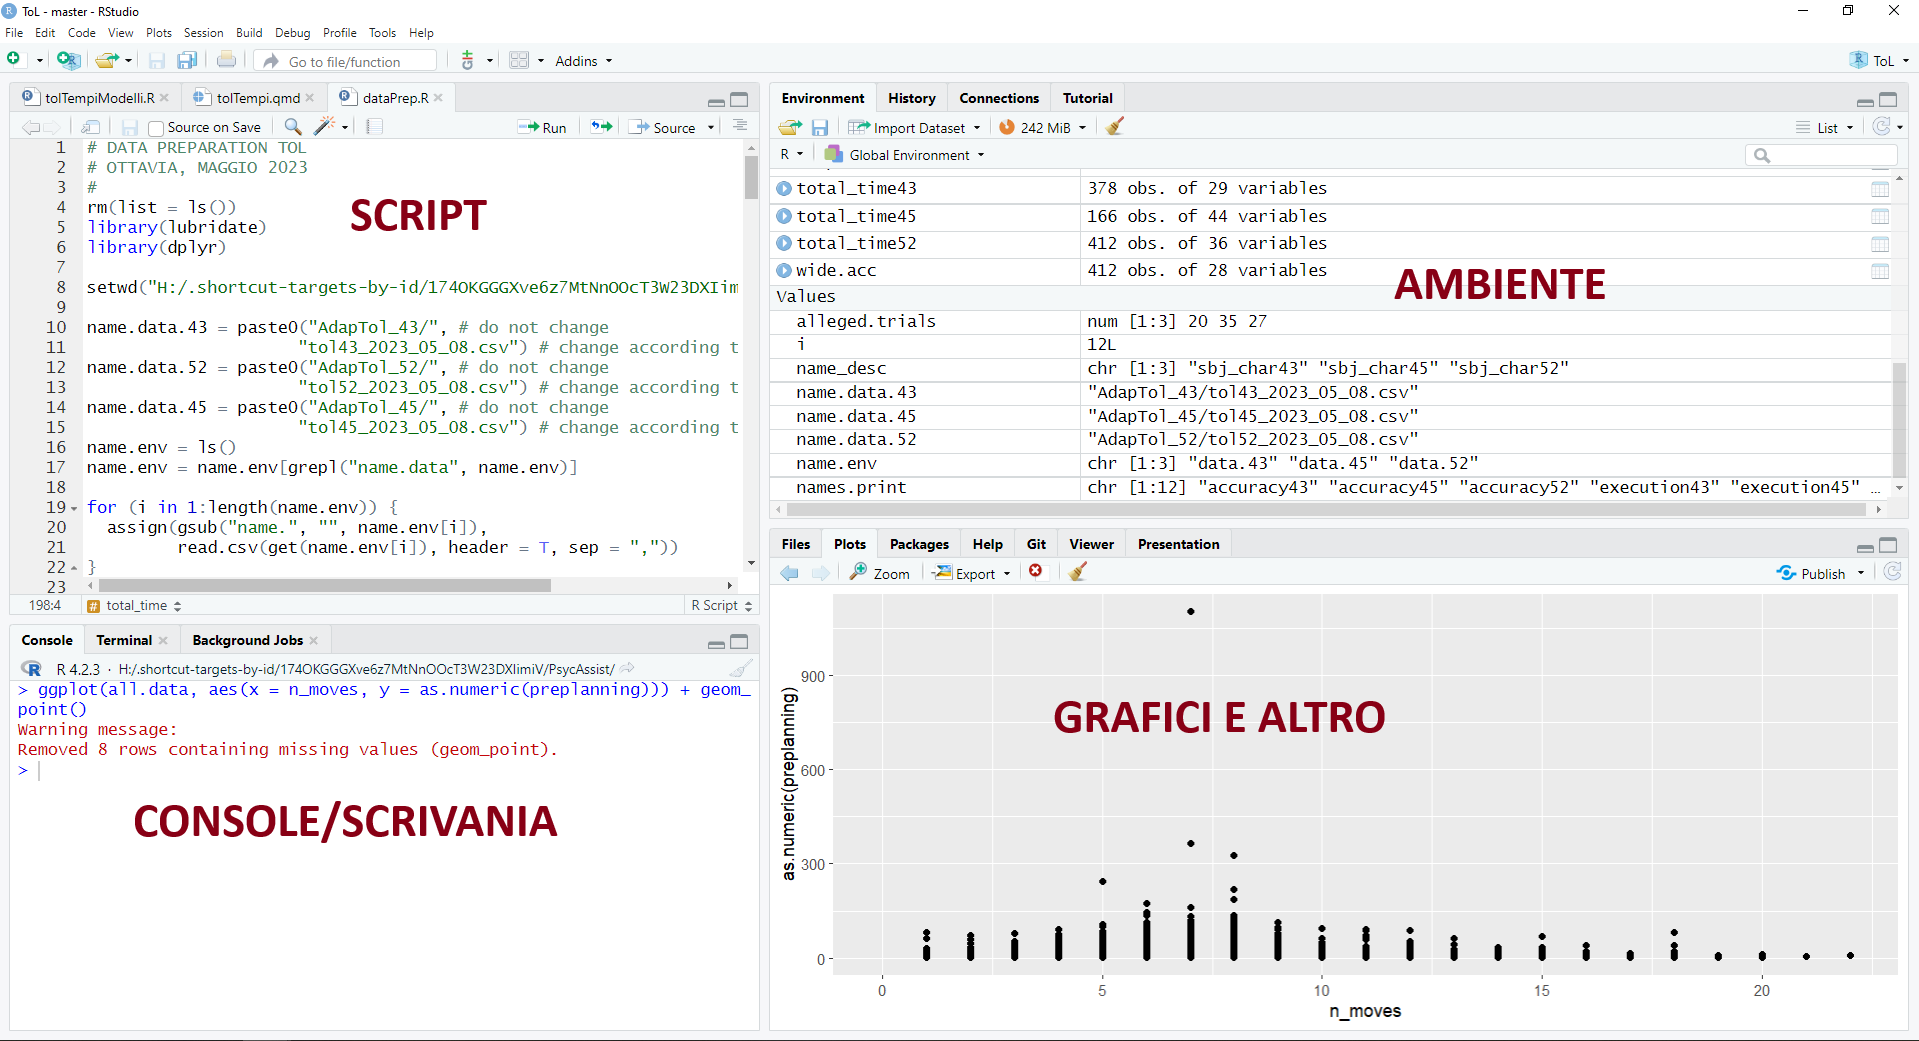
\includegraphics[width=1\linewidth,height=\textheight,keepaspectratio]{slides/modulo1/img/Rstudio.png}
\end{center}

\textbf{Ambiente/Environment} (Pannello in alto a dx). Contiene tutti
gli oggetti che sono stati creati fino a quel momento nell'ambiente di
lavoro. Viene automaticamente suddiviso in oggetti di tipo vettoriale o
scalare (\texttt{values}) e oggetti più complessi come dataframe e
liste.

\textbf{Script}. (Pannelli in alto a sinistra). File di tipo testuale
con estensione \texttt{.R} dove salvare il codice usato per generare gli
oggetti presenti nell'ambiente. Si possono combinare codice e commenti
(righe che non vengono eseguite e interpretate come codice, sono le
righe precedute dal simbolo \texttt{\#}, vedi
Listing~\ref{lst-example}). Per eseguire i comandi negli script bisogna
usare la combinazione di tasti \texttt{ctrl\ +\ invio} (per il mac,
\texttt{cmd\ +\ invio})

\textbf{Console}. (Pannello in basso a sinistra). Pannello di lavoro
dove i lavori vengono immediatamente eseguiti immediatamente quando si
clicca invio. Le righe di comando non vengon salvate ma sono sempre
accessibili premendo con la freccina in su della tastiera. Nella console
appaiono anche i risultati dei codici eseguiti nello script.

\textbf{Plot/Files}. (Pannello in basso a dx). Pannnello composto da
diversi pannelli. Nel pannello \texttt{Plots} compaiono i grafici
risultatinti dalle analisi statistiche svolte negli script. Nel pannello
\texttt{Files} appaiono tutti i file e le cartelle dispoonibili in una
data working directory (Vedi Section~\ref{sec-wd} e
Section~\ref{sec-project}).

\begin{codelisting}

\caption{\label{lst-example}Codice con commento}

\centering{

\begin{Shaded}
\begin{Highlighting}[]
\CommentTok{\# codice per assegnare il numero 25 alla variabile x}
\NormalTok{x }\OtherTok{\textless{}{-}} \DecValTok{25} 
\end{Highlighting}
\end{Shaded}

}

\end{codelisting}%

\begin{tcolorbox}[enhanced jigsaw, toprule=.15mm, left=2mm, leftrule=.75mm, breakable, coltitle=black, title={Console}, bottomtitle=1mm, opacitybacktitle=0.6, toptitle=1mm, titlerule=0mm, bottomrule=.15mm, colframe=quarto-callout-note-color-frame, arc=.35mm, rightrule=.15mm, opacityback=0, colbacktitle=quarto-callout-note-color!10!white, colback=white]

I comandi nella console vengono eseguiti con click su Invio

Il codice non viene salvato e scompare sequenzialmente.

L'output appare immediatamente nella console.

Per fare lo switch alla console \(\rightarrow\) \texttt{ctrl\ +\ 2}

\end{tcolorbox}

\begin{tcolorbox}[enhanced jigsaw, toprule=.15mm, left=2mm, leftrule=.75mm, breakable, coltitle=black, title={Script}, bottomtitle=1mm, opacitybacktitle=0.6, toptitle=1mm, titlerule=0mm, bottomrule=.15mm, colframe=quarto-callout-note-color-frame, arc=.35mm, rightrule=.15mm, opacityback=0, colbacktitle=quarto-callout-note-color!10!white, colback=white]

Si possono salvare gli script di codice

Per far ``correre'' qualsiasi comando nello script \(\rightarrow\) Ctrl
+ Invio (o \texttt{cmd\ +\ Enter})

L'output appare nella console.

Per fare lo switch allo script \(\rightarrow\) \texttt{ctr\ +\ 1}

\end{tcolorbox}

\section{\texorpdfstring{Working directories
(\texttt{wd})}{Working directories (wd)}}\label{sec-wd}

\textbf{Working directory}. La cartella dentro cui sta lavorando R in
quel momento. Diventa di fondamentale importanza perché è dove R si
aspetta che ci siano i file (e.g., i dati) con cui volete lavorare

\subsection{Hard way}\label{hard-way}

\begin{codelisting}

\caption{\label{lst-wd}Funzione per ottenere la wd, ovvero la cartella
dentro cui sta lavorando R}

\centering{

\begin{Shaded}
\begin{Highlighting}[]
\CommentTok{\# per sapere dove sta lavorando R}
\FunctionTok{getwd}\NormalTok{()}
\end{Highlighting}
\end{Shaded}

}

\end{codelisting}%

\begin{verbatim}
[1] "C:/Users/Ottavia/Documents/GitHub/stpc-analisi-dati"
\end{verbatim}

La \texttt{wd} si può cambiare con il comando \texttt{setwd()}:

\begin{codelisting}

\caption{\label{lst-wdSet}Funzione per ottenere cambiare la wd dentro
cui sta lavorando R. Dentro la funzione, va messo il percorso completo
entro cui si vuole spostare la cartella di lavoro tra virgolette, come
nell'esempio sottostante.}

\centering{

\begin{Shaded}
\begin{Highlighting}[]
\FunctionTok{setwd}\NormalTok{(}\StringTok{"C:/Users/Ottavia/Documents/altro{-}percorso"}\NormalTok{)}
\end{Highlighting}
\end{Shaded}

}

\end{codelisting}%

\subsection{Easy Way: R Project}\label{sec-project}

Crea automaticamente una working directory (ovvero una cartella) in cui
potete trovare tutto il materiale necessario per delle analisi. Questo
vi evita di dover pensare alla gestione delle working directories.

Struttura tipica

\begin{Shaded}
\begin{Highlighting}[]
\NormalTok{my{-}project/}
\NormalTok{|}
\NormalTok{+{-}{-} index.qmd}
\NormalTok{+{-}{-} laboratorioTemplate.qmd}
\NormalTok{+{-}{-} myScript.R}
\NormalTok{+{-}{-} my{-}project.Rproj}
\NormalTok{+{-}{-} data/}
\NormalTok{|   +{-}{-} mydata.csv}
\end{Highlighting}
\end{Shaded}

Nell'esempio precedente, la cartella di ordine superiore è la cartella
\texttt{my-project}, ovvero la cartella che contiene tutto il vostro
progetto. Al suo iinterno si trovano i seguenti file, a diversi livelli:

\begin{enumerate}
\def\labelenumi{\arabic{enumi}.}
\tightlist
\item
  Primo Livello: \texttt{index.qmd}, \texttt{laboratorioTemplate.qmd},
  \texttt{myScript.R} (file di quarto con estensione \texttt{qmd}, file
  R con estensione \texttt{R}) e una cartella \texttt{data}. Il file
  \texttt{my-project.Rproj} è il file del vostro progetto R con
  estensione \texttt{Rproj}.
\item
  Secondo Livello: all'interno della cartella \texttt{data} si trova il
  file \texttt{mydata.csv}. Per accedere a questo file di dati da un
  file contenuto nella cartella di ordine superiore, bisogna
  semplicemente comunicare a R che si trova nella cartella data,
  \texttt{"data/mydata.csv"}.
\end{enumerate}

\subsubsection{Creare un nuovo progetto}\label{creare-un-nuovo-progetto}

Da \texttt{File} \(\rightarrow\) New Project e seguire i seguenti step:

\begin{figure}

\begin{minipage}{0.33\linewidth}

\centering{

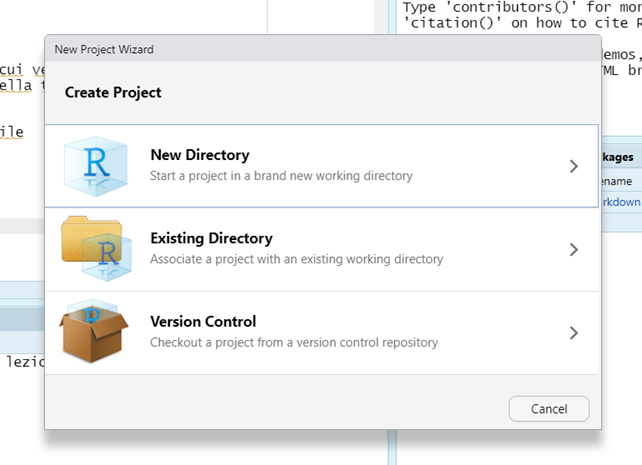
\includegraphics[width=1\linewidth,height=\textheight,keepaspectratio]{slides/modulo1/img/project1.png}

}

\subcaption{\label{fig-project-1}Step 1}

\end{minipage}%
%
\begin{minipage}{0.33\linewidth}

\centering{

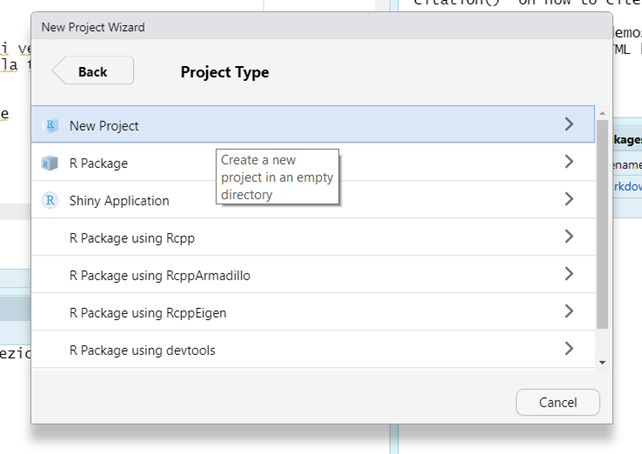
\includegraphics[width=1\linewidth,height=\textheight,keepaspectratio]{slides/modulo1/img/project2.png}

}

\subcaption{\label{fig-project-2}Step 2}

\end{minipage}%
%
\begin{minipage}{0.33\linewidth}

\centering{

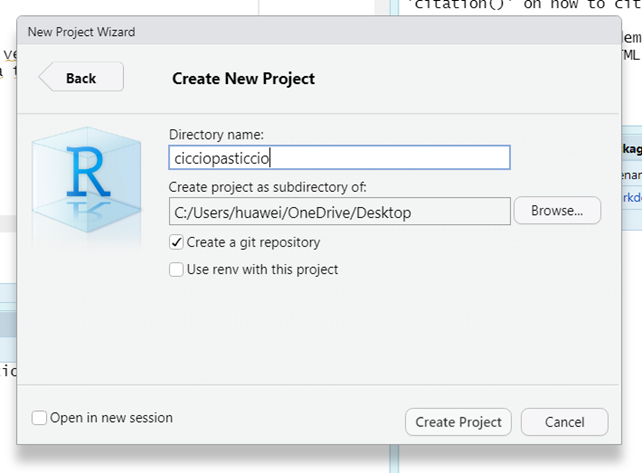
\includegraphics[width=1\linewidth,height=\textheight,keepaspectratio]{slides/modulo1/img/project3.png}

}

\subcaption{\label{fig-project-3}Step 3}

\end{minipage}%

\caption{\label{fig-project}Creare un progetto R in 3 step}

\end{figure}%

In Figure~\ref{fig-project-1} selezionare l'opzione
\texttt{New\ directory}.

In Figure~\ref{fig-project-2} selezionare l'opzione
\texttt{New\ Project} (ignorate tutte le altre opzioni).

In Figure~\ref{fig-project-3} date un nome al progetto (e.g.,
\texttt{corso-analisi}) e secgliete la cartella entro cui salvarlo
(consigliato: I Documenti del vostro computer).

Figure~\ref{fig-pjCheck} illsutra il controllo per capire se
effettivamente siete dentro al progetto R. Se non siete dentro il
progetto R, andate a cercarlo nella cartella dove lo avete creato e fate
doppio click sul file con estensione \texttt{Rproj}.

\begin{figure}

\centering{


\includegraphics[width=0.7\linewidth,height=\textheight,keepaspectratio]{slides/modulo1/img/progetto.png}

}

\caption{\label{fig-pjCheck}Indica il nome del progetto}

\end{figure}%

\section{Script e reporting}\label{script-e-reporting}

Figure~\ref{fig-newScript} illustra come creare un nuovo script, dove è
possibile eseguire e salvare una serie di comandi.

\begin{figure}

\centering{

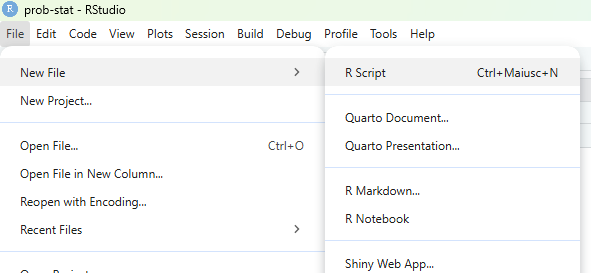
\includegraphics[width=0.7\linewidth,height=\textheight,keepaspectratio]{slides/modulo1/img/new-script.png}

}

\caption{\label{fig-newScript}Creare un nuovo script}

\end{figure}%

In alternativa, si può usare la sequenza di tasti:
\texttt{Ctrl\ +\ shift\ +\ n} (\texttt{cmd\ +\ shift\ +\ n})

Per salvare uno script, bastare cliccare sull'icona del salvataggio.

\section{Reporting con quarto}\label{reporting-con-quarto}

quarto è un markup language integrato con RStudio.

Permette la creazione di documenti (sia pdf sia html) che possono
contenere chunk di codice, ovvero delle parti dove viene eseguito il
codice R, per ottenere risultati, tabelle e grafici.

In questo corso, useremo quarto per tutti gli esercizi. Vi verranno
forniti dei template, specie all'inizio, nella speranza che riusciate a
modificarli e a diventare via via più autonome nel suo utilizzo.

Una parte dell'esame prevede l'utilizzo di quarto per lo svolgimento
degli esercizi. le esercitazioni in intinere sono da svolgere su quarto.

A \href{https://arca-dpss.github.io/shine-with-quarto/}{questo link}
trovate maggiori informazioni su quarto e una guida veloce sul suo
funzionamento.

Figure~\ref{fig-quarto-1} crea un nuovo file quarto, mentre
Figure~\ref{fig-quarto-2} illustra come specificare varie opzioni del
docuemnto (titolo, autrice).

\begin{figure}

\caption{\label{fig-quarto}Crea un nuovo file quarto}

\begin{minipage}{0.50\linewidth}

\centering{

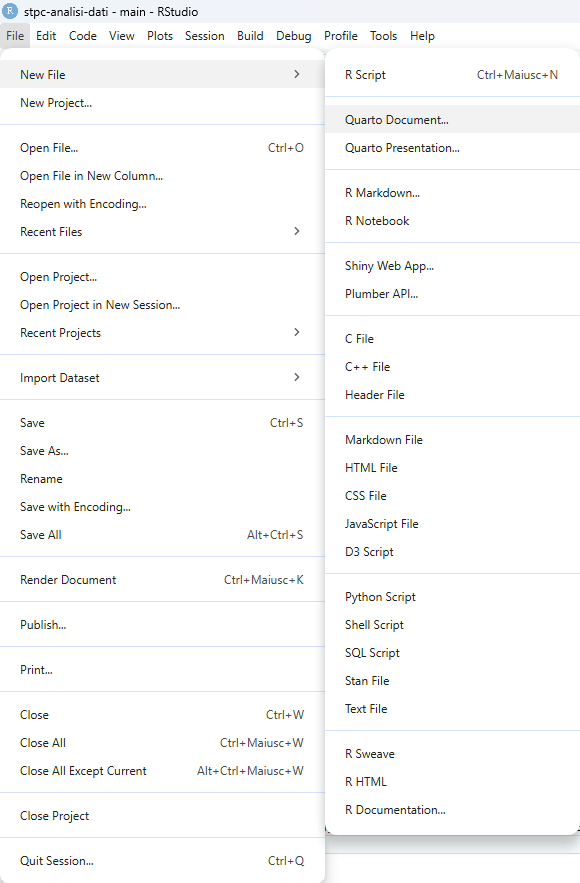
\includegraphics[width=1\linewidth,height=\textheight,keepaspectratio]{slides/modulo1/img/quarto0.png}

}

\subcaption{\label{fig-quarto-1}Crea il file}

\end{minipage}%
%
\begin{minipage}{0.50\linewidth}

\centering{

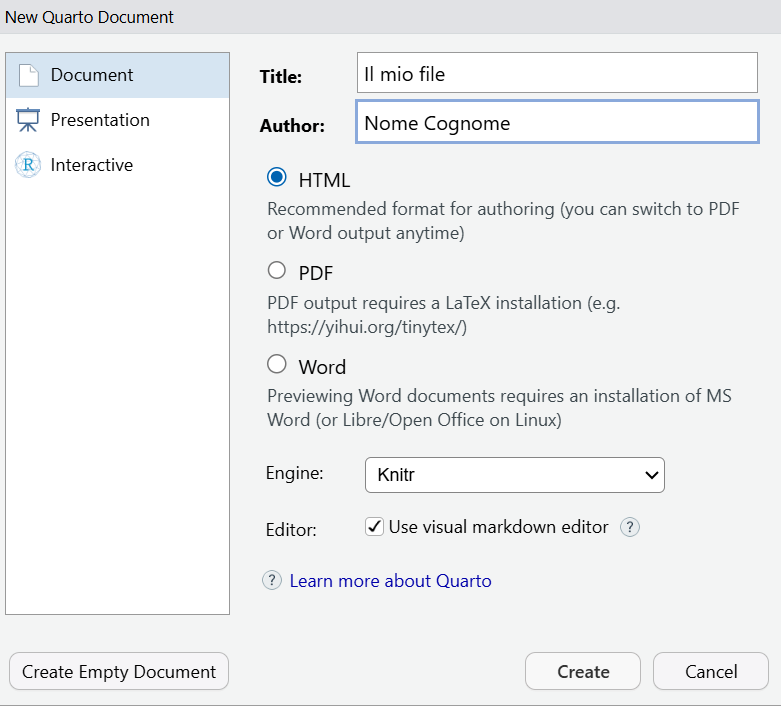
\includegraphics[width=1\linewidth,height=\textheight,keepaspectratio]{slides/modulo1/img/quarto1.png}

}

\subcaption{\label{fig-quarto-2}Selezione tipo di file/dati}

\end{minipage}%

\end{figure}%

Figure~\ref{fig-example} vi mostra il default che si ottiene quando si
crea un documento quarto.

\begin{figure}

\centering{

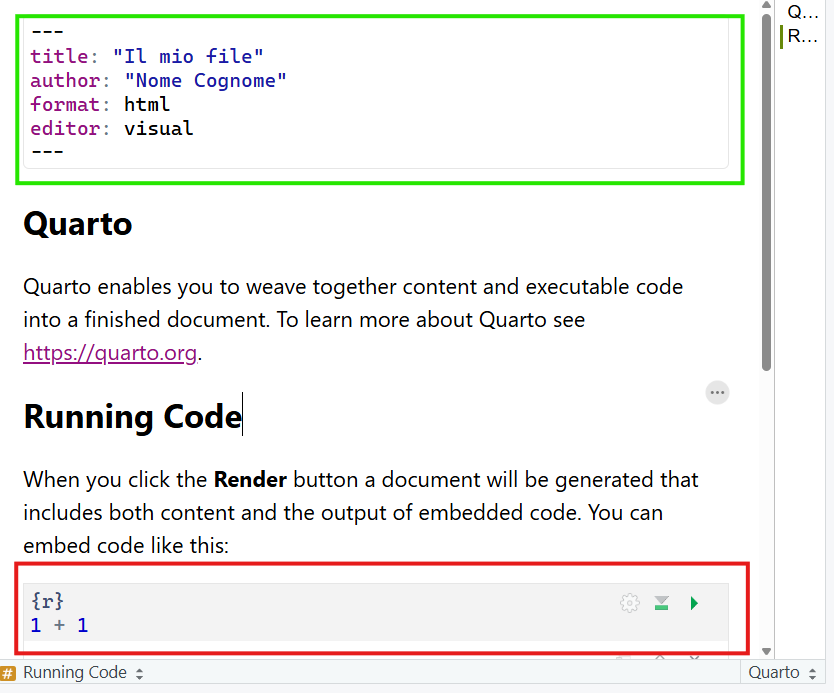
\includegraphics[width=0.7\linewidth,height=\textheight,keepaspectratio]{slides/modulo1/img/quarto2.png}

}

\caption{\label{fig-example}Deafult documento di quarto. In verde lo
YAML, in rosso un chunk di codice eseguibile come qualsiasi script R}

\end{figure}%

In verde in Figure~\ref{fig-example}, lo YAML che controlla l'aspetto
generale del documento. Va modificato per cambiare i metadati del
documento.

In rosso in Figure~\ref{fig-example}, un chunk di codice eseguibile,
ovvero una parte del docuemnto che funziona come un qualsaisi script di
R e in quanto tale permette di esguire codice.

\begin{tcolorbox}[enhanced jigsaw, toprule=.15mm, left=2mm, leftrule=.75mm, breakable, coltitle=black, title={Modifica importante allo YAML}, bottomtitle=1mm, opacitybacktitle=0.6, toptitle=1mm, titlerule=0mm, bottomrule=.15mm, colframe=quarto-callout-caution-color-frame, arc=.35mm, rightrule=.15mm, opacityback=0, colbacktitle=quarto-callout-caution-color!10!white, colback=white]

La parte \texttt{embed-resources:\ true} è fondamentale (e va scritta
esattamente seguento l'indentazione riportata). Serve a fare in modo che
tutti i codici, i risultati e i grafici prodotti nel documento rimangano
nel documento quando lo compilate in html.

\begin{Shaded}
\begin{Highlighting}[]
\CommentTok{{-}{-}{-}}
\AnnotationTok{title:}\CommentTok{ "Il mio file"}
\AnnotationTok{author:}\CommentTok{ "Nome Cognome"}
\AnnotationTok{format:}\CommentTok{ }
\CommentTok{  html: }
\CommentTok{   embed{-}resources: true}
\AnnotationTok{editor:}\CommentTok{ visual}
\CommentTok{{-}{-}{-}}
\end{Highlighting}
\end{Shaded}

\end{tcolorbox}

Il chunk di codice funziona esattamente come R -- è sequenziale, va
seguito l'ordine con cui vengono fatte le operazioni

Ogni volta che viene fatto il rendering del documento
(\texttt{shift\ +\ ctrl\ +\ k} o freccina azzurra), viene creato un
ambiente temporaneo dove viene eseguito il codice.

L'ambiente temporaneo è indipendente dall'ambiente che vedete su R!

Per creare un nuovo chunk: \texttt{shift\ +\ ctrl\ +\ i} oppure
Figure~\ref{fig-chunk}:

\begin{figure}

\centering{

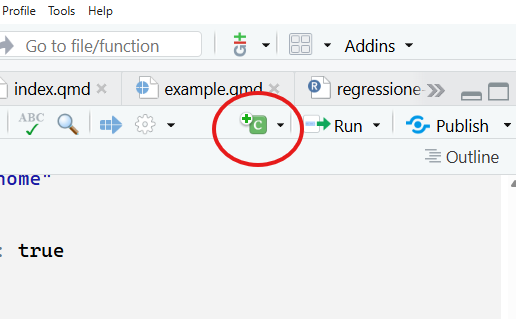
\includegraphics[width=0.5\linewidth,height=\textheight,keepaspectratio]{slides/modulo1/img/chunk.png}

}

\caption{\label{fig-chunk}Creare un nuovo chunk di codice}

\end{figure}%

\section{Elementi base}\label{elementi-base}

\subsection{Calcolatrice}\label{calcolatrice}

\begin{Shaded}
\begin{Highlighting}[]
\DecValTok{3} \SpecialCharTok{+} \DecValTok{2}   \CommentTok{\# più}
\DecValTok{3} \SpecialCharTok{{-}} \DecValTok{2}   \CommentTok{\# meno}
\DecValTok{3} \SpecialCharTok{*} \DecValTok{2}   \CommentTok{\# per}
\DecValTok{3} \SpecialCharTok{/} \DecValTok{2}   \CommentTok{\# diviso}
\end{Highlighting}
\end{Shaded}

Parentesi e simili:

\begin{quote}
\texttt{()} \texttt{{[}{]}} \texttt{\{\}} \texttt{""} \texttt{:}
\texttt{;} \texttt{,}
\end{quote}

\begin{tcolorbox}[enhanced jigsaw, toprule=.15mm, left=2mm, leftrule=.75mm, breakable, coltitle=black, title={ATTENZIONE}, bottomtitle=1mm, opacitybacktitle=0.6, toptitle=1mm, titlerule=0mm, bottomrule=.15mm, colframe=quarto-callout-caution-color-frame, arc=.35mm, rightrule=.15mm, opacityback=0, colbacktitle=quarto-callout-caution-color!10!white, colback=white]

Nei chunk di codice che seguono vedrete spesso l'operatore \texttt{;}
scritto sulla stessa riga di codice dove viene eseguita un'altra
operazione, come ad esempio:

\begin{Shaded}
\begin{Highlighting}[]
\NormalTok{variabile }\OtherTok{=} \DecValTok{1}\SpecialCharTok{:}\DecValTok{5}\NormalTok{ ; variabile}
\end{Highlighting}
\end{Shaded}

\begin{verbatim}
[1] 1 2 3 4 5
\end{verbatim}

equivale a scrivere

\begin{Shaded}
\begin{Highlighting}[]
\NormalTok{variabile }\OtherTok{=} \DecValTok{1}\SpecialCharTok{:}\DecValTok{5} 
\NormalTok{variabile}
\end{Highlighting}
\end{Shaded}

\begin{verbatim}
[1] 1 2 3 4 5
\end{verbatim}

\end{tcolorbox}

\subsection{Assign (Crea oggetti)}\label{assign-crea-oggetti}

Tutto quello che viene creato in R viene chiamato \emph{oggetto} tramite
l'\,``assegnazione'' con specifici simboli, ovvero \texttt{\textless{}-}
oppure \texttt{=}:

\begin{Shaded}
\begin{Highlighting}[]
\NormalTok{x }\OtherTok{\textless{}{-}} \DecValTok{4} 
\NormalTok{x }
\end{Highlighting}
\end{Shaded}

\begin{verbatim}
[1] 4
\end{verbatim}

\begin{Shaded}
\begin{Highlighting}[]
\NormalTok{X }\OtherTok{=} \DecValTok{5} 
\NormalTok{X}
\end{Highlighting}
\end{Shaded}

\begin{verbatim}
[1] 5
\end{verbatim}

Gli elementi a destra del simbolo (contenuto) vengono assegnati
all'elemento a sinsitra (contenitore) del simbolo

\begin{tcolorbox}[enhanced jigsaw, toprule=.15mm, left=2mm, leftrule=.75mm, breakable, coltitle=black, title={Attenzione!}, bottomtitle=1mm, opacitybacktitle=0.6, toptitle=1mm, titlerule=0mm, bottomrule=.15mm, colframe=quarto-callout-warning-color-frame, arc=.35mm, rightrule=.15mm, opacityback=0, colbacktitle=quarto-callout-warning-color!10!white, colback=white]

R è case sensitive. \texttt{x} e \texttt{X} sono due oggetti diversi!

\end{tcolorbox}

\subsection{Nominare gli oggetti}\label{nominare-gli-oggetti}

\begin{center}
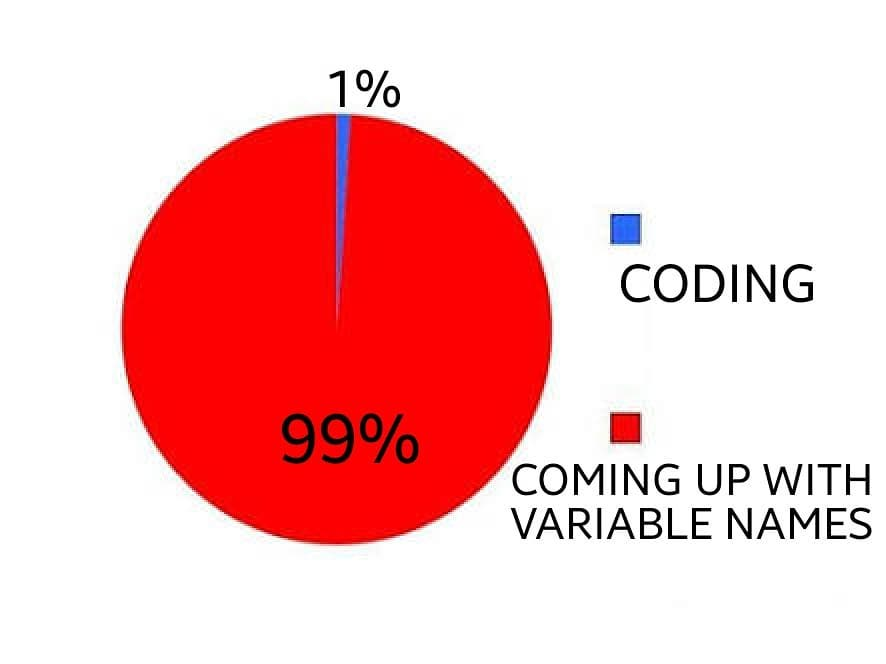
\includegraphics[width=0.25\linewidth,height=\textheight,keepaspectratio]{slides/modulo1/img/meme.jpg}
\end{center}

Nomi validi sono lettere, numeri, punti, underscore (e.g.,
\texttt{variable\_name})

Buoni nomi per le variabili:

\begin{itemize}
\item
  \texttt{mean\_rt}
\item
  \texttt{sum\_age}
\item
  \texttt{prop\_item}
\end{itemize}

Pessimi nomi per variabili:

\begin{itemize}
\item
  \texttt{x}
\item
  \texttt{y}
\item
  \texttt{ciccio}
\end{itemize}

Non deve contenere caratteri speciali come \#, \&, \$, ?, etc.

Non deve essere una parola riservata ovvero quelle parole che sono
utilizzate da R con un significato speciale (\texttt{?reserved} nella
console).

\begin{Shaded}
\begin{Highlighting}[]
\NormalTok{.}\DecValTok{01} \OtherTok{=} \DecValTok{5}
\end{Highlighting}
\end{Shaded}

\begin{verbatim}
Error in 0.01 = 5: membro di sinistra dell'assegnazione (do_set) non valido
\end{verbatim}

\begin{Shaded}
\begin{Highlighting}[]
\DecValTok{1} \OtherTok{=} \StringTok{"a"}
\end{Highlighting}
\end{Shaded}

\begin{verbatim}
Error in 1 = "a": membro di sinistra dell'assegnazione (do_set) non valido
\end{verbatim}

\begin{Shaded}
\begin{Highlighting}[]
\ConstantTok{TRUE} \OtherTok{=} \DecValTok{567}
\end{Highlighting}
\end{Shaded}

\begin{verbatim}
Error in TRUE = 567: membro di sinistra dell'assegnazione (do_set) non valido
\end{verbatim}

\subsubsection{Per convenzione}\label{per-convenzione}

Queste istruzioni sono valide attraverso diversi linguaggi di
programmazione.

Fanno riferimento a nomi di oggetti composti da più nomi e/o molto
lunghi:

\begin{enumerate}
\def\labelenumi{\arabic{enumi}.}
\tightlist
\item
  \texttt{first\_data}, ovvero separare i termini con un underscore
  (e.g., \texttt{my\_data})
\item
  \texttt{firstData}, ovvero la prima parola tutta minuscola, la seconda
  con la prima lettera maiuscola (e.g., \texttt{unitnData} invece di
  \texttt{university\_of\_trento\_data})
\end{enumerate}

\subsection{L'ambiente}\label{lambiente}

Gli oggetti finiscono nell'ambiente (\texttt{environment}) di R.

La funzione \texttt{ls()} permette di vedere tutti gli oggetti
all'interno dell'ambiente.

\begin{figure}[H]

{\centering 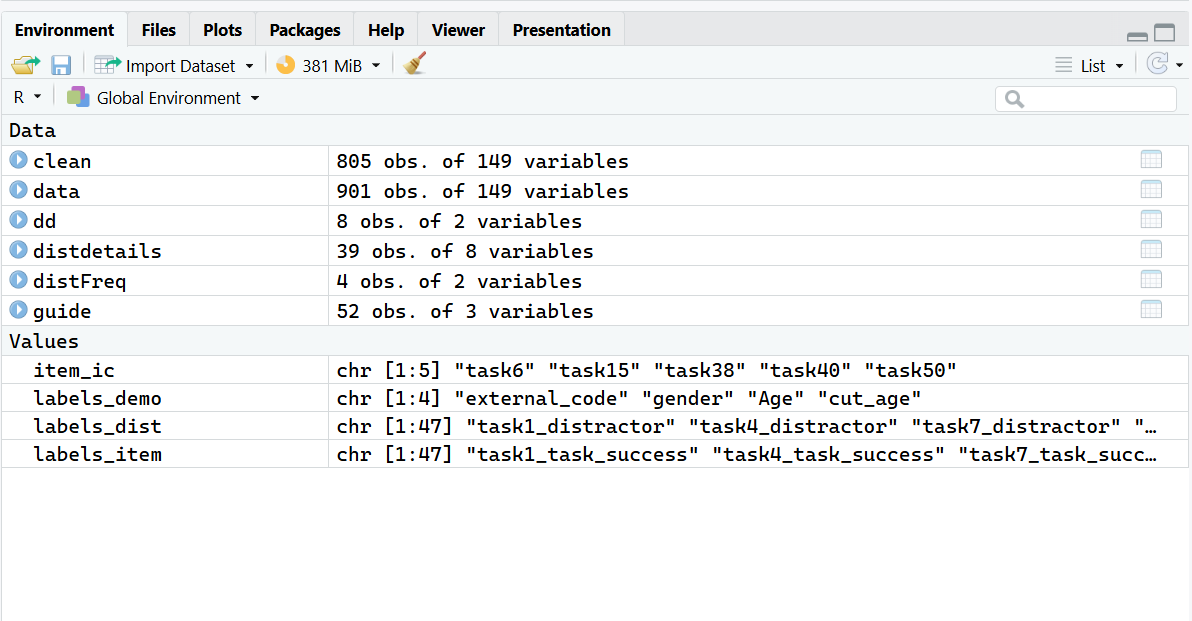
\includegraphics[width=0.7\linewidth,height=\textheight,keepaspectratio]{slides/modulo1/img/env.png}

}

\caption{Ambiente di R}

\end{figure}%

\texttt{rm()} (remove) è la funzione preposta per rimuovere gli oggetti
dall'ambiente di R: \texttt{rm("oggetto")} (vedi Listing~\ref{lst-env}).

Il codice \texttt{rm(list\ =\ ls())} permette di eliminare tutti gli
oggetti nell'ambiente in un colpo solo (equivale alla scopetta).

\begin{codelisting}

\caption{\label{lst-env}Ottenere gli elementi nell'ambiente e uso della
funzione rm}

\centering{

\begin{Shaded}
\begin{Highlighting}[]
\FunctionTok{ls}\NormalTok{() }\CommentTok{\# ottiene tutti gli oggetti nell\textquotesingle{}ambiente}
\end{Highlighting}
\end{Shaded}

}

\end{codelisting}%

\begin{verbatim}
[1] "variabile" "x"         "X"        
\end{verbatim}

\begin{codelisting}

\caption{\label{lst-env}Ottenere gli elementi nell'ambiente e uso della
funzione rm}

\centering{

\begin{Shaded}
\begin{Highlighting}[]
\FunctionTok{rm}\NormalTok{(variabile) }\CommentTok{\# rimuove l\textquotesingle{}oggetto variabile }
\FunctionTok{ls}\NormalTok{()}
\end{Highlighting}
\end{Shaded}

}

\end{codelisting}%

\begin{verbatim}
[1] "x" "X"
\end{verbatim}

\begin{codelisting}

\caption{\label{lst-env}Ottenere gli elementi nell'ambiente e uso della
funzione rm}

\centering{

\begin{Shaded}
\begin{Highlighting}[]
\FunctionTok{rm}\NormalTok{(}\AttributeTok{list =} \FunctionTok{ls}\NormalTok{()) }\CommentTok{\# rimuove tutto l\textquotesingle{}ambiente}
\FunctionTok{ls}\NormalTok{()}
\end{Highlighting}
\end{Shaded}

}

\end{codelisting}%

\begin{verbatim}
character(0)
\end{verbatim}

\section{Pacchetti e Funzioni}\label{pacchetti-e-funzioni}

\subsection{Funzioni}\label{funzioni}

Ogni cosa fatta in R di fatto è riassumbile nelle \emph{operazioni}
fatte su \emph{oggetti}

Le operazioni sono le \textbf{funzioni}, che permettono di modificare
gli oggetti esistenti e di creare di nuovi.

Ad esempio, in Listing~\ref{lst-sum} viene usata la funzione
\texttt{sum()} per sommare tutti gli elementi all'interno del vettore.
Matematicamente, la funzione \texttt{sum()} equivale a
\(\displaystyle \sum_{i = 1}^k x_i\) dove \(k\) è il totale di elementi
\(x\) all'interno del vettore \(X\).

\begin{codelisting}

\caption{\label{lst-sum}Applica la funzione somma per sommare tutti gli
elementi all'interno di vettore}

\centering{

\begin{Shaded}
\begin{Highlighting}[]
\NormalTok{vettore }\OtherTok{=} \DecValTok{1}\SpecialCharTok{:}\DecValTok{5}
\FunctionTok{sum}\NormalTok{(vettore)}
\end{Highlighting}
\end{Shaded}

}

\end{codelisting}%

\begin{verbatim}
[1] 15
\end{verbatim}

Le funzioni in R sono come le funzioni matematiche \(f(\cdot)\), dove
viene preso un input, viene elaborato secondo le regole della funzione e
si ottiene un output:

\begin{center}
\pandocbounded{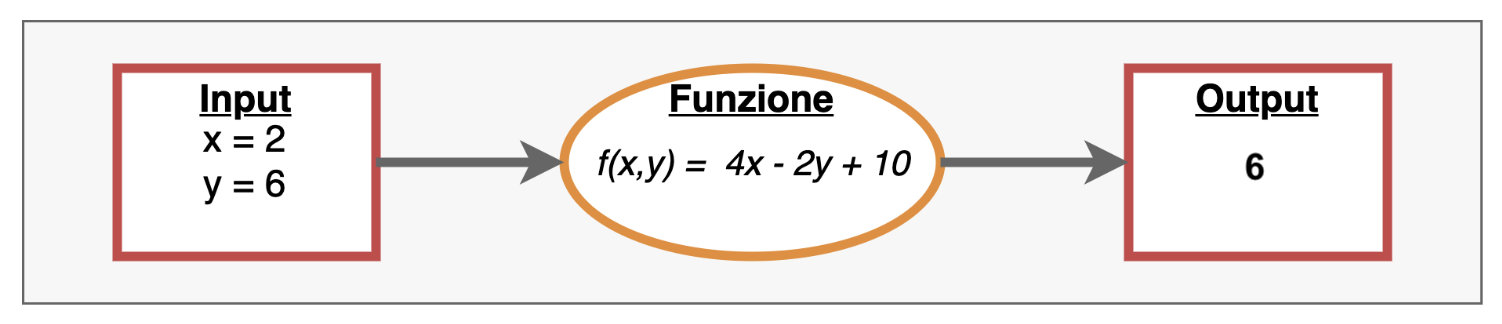
\includegraphics[keepaspectratio]{slides/modulo1/img/fun1.png}}
\end{center}

\subsubsection{Elementi di una funzione}\label{elementi-di-una-funzione}

\begin{verbatim}
mean(x, trim = 0, na.rm = FALSE, ...)
\end{verbatim}

\begin{itemize}
\tightlist
\item
  Nome della funzione: \texttt{mean}
\item
  Parentesi che racchiudono gli argomenti della funzione
\item
  argomenti:

  \begin{itemize}
  \tightlist
  \item
    \textbf{obbligatori}, senza valori predefiniti senza di cui la
    funzione non può funzionare. Nel caso della funzione
    \texttt{mean()}, l'unico argomento obbligatorio è il vettore
    \texttt{x} di valori di cui si vuole calcolare la media
  \item
    \textbf{facoltativi} con valori di default (\texttt{trim\ =\ 0},
    \texttt{na.rm\ =\ FALSE}), che vangono applicati qualora l'utente
    non ne specifichi di alternativi. Nel caso della media, non viene
    applicato il trimming dei valori estremi e non vengono tolti i
    valori NA.
  \end{itemize}
\end{itemize}

\begin{Shaded}
\begin{Highlighting}[]
\FunctionTok{mean}\NormalTok{(vettore)}
\end{Highlighting}
\end{Shaded}

\begin{verbatim}
[1] 3
\end{verbatim}

\begin{Shaded}
\begin{Highlighting}[]
\FunctionTok{mean}\NormalTok{(vettore, }\AttributeTok{trim =} \FloatTok{0.3}\NormalTok{)}
\end{Highlighting}
\end{Shaded}

\begin{verbatim}
[1] 3
\end{verbatim}

\texttt{?funzione} (Listing~\ref{lst-help}) permette di accedere
all'help della funzione per scoprire esattamente cosa fa una funzione:

\begin{codelisting}

\caption{\label{lst-help}Permette di accedere all'help della funzione
mean}

\centering{

\begin{Shaded}
\begin{Highlighting}[]
\NormalTok{?mean}
\end{Highlighting}
\end{Shaded}

}

\end{codelisting}%

\begin{figure}[H]

{\centering 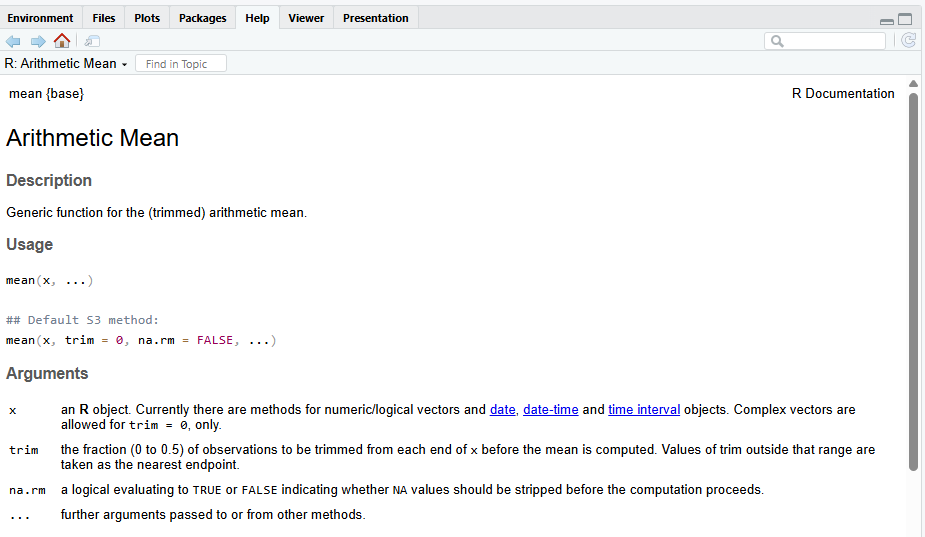
\includegraphics[width=1\linewidth,height=\textheight,keepaspectratio]{slides/modulo1/img/mean.png}

}

\caption{Help della funzione mean}

\end{figure}%

\subsubsection{Installare i pacchetti}\label{installare-i-pacchetti}

Esistono funzioni predefinite all'installazione di R, se ne possono
definire di nuove autonomamente, si possono installare dei ``pacchetti''
dal CRAN (comprehensive R archive network, vedi
Listing~\ref{lst-install}) o da un file locale, a seconda delle
operazioni che si vogliono svolgere.

\begin{codelisting}

\caption{\label{lst-install}Codice per installare e caricare un
pacchetto}

\centering{

\begin{Shaded}
\begin{Highlighting}[]
\FunctionTok{install.packages}\NormalTok{(}\StringTok{"nomePacchetto"}\NormalTok{) }\CommentTok{\# installa (va fatto correre solo una volta)}
\FunctionTok{library}\NormalTok{(nomePacchetto) }\CommentTok{\# carica il pacchetto (va fatto correre tutte le volte)}
\end{Highlighting}
\end{Shaded}

}

\end{codelisting}%

\section{Operatori}\label{operatori}

\subsection{Operatori Matematici}\label{operatori-matematici}

Tabella \ref{tbl-operatori} illustra alcuni operatori matematici di
base, mentre Tabella \ref{tbl-funzioni-matematiche} illustrate le
principali funzioni matematiche disponibili in R.

\begin{table}[htbp]
\centering
\caption{Operatori matematici in R}
\label{tbl:operatori}
\begin{tabular}{llll}
\toprule
Funzione & Cosa fa? & Esempio & Risultato \\
\midrule
\texttt{+}      & addizione       & \texttt{5.4 + 6.1}    & \texttt{11.5} \\
\texttt{-}      & sottrazione     & \texttt{9 - 4.3}      & \texttt{4.7}  \\
\texttt{*}      & moltiplicazione & \texttt{7 * 1.4}      & \texttt{9.8}  \\
\texttt{/}      & divisione       & \texttt{9/3}          & \texttt{3}    \\
\texttt{\%\%}   & resto           & \texttt{9\%\%2}       & \texttt{1}    \\
\texttt{\^{}}   & potenza         & \texttt{15 \^{} 2}    & \texttt{225}  \\
\bottomrule
\end{tabular}
\end{table}

\begin{table}[htbp]
\centering
\caption{Funzioni matematiche in R}
\label{tbl:funzioni-matematiche}
\begin{tabular}{llll}
\toprule
Funzione & Cosa fa? & Esempio & Risultato \\
\midrule
\texttt{abs()}   & valore assoluto        & \texttt{abs(-8)}         & \texttt{8}    \\
\texttt{sqrt()}  & radice quadrata        & \texttt{sqrt(225)}       & \texttt{15}   \\
\texttt{exp()}   & funzione esponenziale  & \texttt{exp(0)}          & \texttt{1}    \\
\texttt{log()}   & logaritmo naturale     & \texttt{log(1)}          & \texttt{0}    \\
\texttt{round()} & arrotondamento, intero & \texttt{round(1.738)}    & \texttt{2}    \\
\texttt{round()} & arrotondamento         & \texttt{round(1.738, 2)} & \texttt{1.74} \\
\bottomrule
\end{tabular}
\end{table}

\subsection{Operatori Relazionali}\label{operatori-relazionali}

In R è possibile valutare se una data relazione è vera o falsa. R
valuterà le proposizioni e ci restituirà il valore
\textbf{\texttt{TRUE}} se la proposizione è vera oppure
\textbf{\texttt{FALSE}} se la proposizione è falsa. Per fare questo si
usano gli operatori relazionali in Tabella
\ref{tbl-operatori-relazionali}.

\begin{table}[htbp]
\centering
\caption{Operatori relazionali in R}
\label{tbl:operatori-relazionali}
\begin{tabular}{llll}
\toprule
Funzione & Nome & Esempio & Risultato \\
\midrule
\texttt{==} & uguale  & \texttt{30 == 30} & \texttt{TRUE}  \\
\texttt{!=} & diverso & \texttt{30 != 30} & \texttt{FALSE} \\
\multirow{2}{*}{\texttt{>} / \texttt{>=}} & \multirow{2}{*}{maggiore / maggiore o uguale}
            & \texttt{30 > 10}  & \texttt{TRUE}  \\
            &  & \texttt{30 >= 10} & \texttt{TRUE}  \\
\multirow{2}{*}{\texttt{<} / \texttt{<=}} & \multirow{2}{*}{minore / minore o uguale}
            & \texttt{30 < 10}  & \texttt{FALSE} \\
            &  & \texttt{10 <= 10} & \texttt{TRUE}  \\
\texttt{\%in\%} & inclusione & \texttt{10 \%in\% c(1, 2, 10)} & \texttt{TRUE} \\
\bottomrule
\end{tabular}
\end{table}

\subsection{Insiemistici}\label{insiemistici}

Per capire gli operatori insiemistici (Tabella
\ref{tbl-operatori-logici}), definiziamo un oggetto, \texttt{x}, come
segue:

\begin{Shaded}
\begin{Highlighting}[]
\NormalTok{x }\OtherTok{=} \DecValTok{30} 
\end{Highlighting}
\end{Shaded}

Gli operatori insiemistici permettono di testare diverse condizioni.

\begin{table}

\caption{\label{tbl-operatori-logici}Operatori logici in R (con x = 30)}

\centering{

\centering


\begin{tabular}{llll}
\toprule
Funzione & Nome & Esempio & Risultato \\
\midrule
\texttt{\&} & Congiunzione           & \texttt{x > 25 \& x < 60} & \texttt{TRUE} \\
\texttt{|}  & Disgiunzione inclusiva & \texttt{x > 25 | x > 60}  & \texttt{TRUE} \\
\texttt{!}  & Negazione              & \texttt{!(x < 18)}        & \texttt{TRUE} \\
\bottomrule
\end{tabular}

}

\end{table}%

La \textbf{congiunzione} testa che siano contemporaneamente vere
entrambe le condizioni, ovvero restituisisce un risultato vero se e solo
se entrambe le condizioni sono vere.

La \textbf{congiunzione} testa che sia vera almeno una delle condizioni,
ovvero restituisisce un risultato vero se almeno una delle condizioni è
vera.

La \textbf{negazione} inverte il valore logico.

\section{Tavole di verità}\label{tavole-di-verituxe0}

\begin{longtable}[]{@{}
  >{\raggedright\arraybackslash}p{(\linewidth - 6\tabcolsep) * \real{0.3000}}
  >{\centering\arraybackslash}p{(\linewidth - 6\tabcolsep) * \real{0.2250}}
  >{\centering\arraybackslash}p{(\linewidth - 6\tabcolsep) * \real{0.1500}}
  >{\raggedright\arraybackslash}p{(\linewidth - 6\tabcolsep) * \real{0.3250}}@{}}
\toprule\noalign{}
\begin{minipage}[b]{\linewidth}\raggedright
Operazione
\end{minipage} & \begin{minipage}[b]{\linewidth}\centering
Simbolo
\end{minipage} & \begin{minipage}[b]{\linewidth}\centering
In R
\end{minipage} & \begin{minipage}[b]{\linewidth}\raggedright
Significato
\end{minipage} \\
\midrule\noalign{}
\endhead
\bottomrule\noalign{}
\endlastfoot
Congiunzione (AND) & \(A \cap B\) & \texttt{\&} & Vera se entrambe le
condizioni sono vere Table~\ref{tbl-tables-1}. \\
Disgiunzione (OR) & \(A \cup B\) & \texttt{\textbar{}} & Vera se almeno
una delle due condizioni è vera Table~\ref{tbl-tables-2}. \\
Negazione (NOT) & \(\overline{A}\) & \texttt{!} & Inverte il valore
logico di \(A\) Table~\ref{tbl-tables-3}. \\
Differenza simmetrica (XOR) & \(A \Delta B\) & \texttt{xor(A,\ B)} &
Vera se una e una sola delle due condizioni è vera
Table~\ref{tbl-tables-4}. \\
\end{longtable}

\begin{table}

\caption{\label{tbl-tables}Tavole di verità}

\begin{minipage}{0.50\linewidth}

\subcaption{\label{tbl-tables-1}Congiunzione}

\centering{

\begin{tabular}{lll}
\toprule
\(a\) & \(b\) & \(a \cap b\)\\
\midrule
V & V & V\\
V & F & F\\
F & V & F\\
F & F & F\\
\bottomrule
\end{tabular}

}

\end{minipage}%
%
\begin{minipage}{0.50\linewidth}

\subcaption{\label{tbl-tables-2}Disgiunzione}

\centering{

\begin{tabular}{lll}
\toprule
\(a\) & \(b\) & \(a \cup b\)\\
\midrule
V & V & V\\
V & F & V\\
F & V & V\\
F & F & F\\
\bottomrule
\end{tabular}

}

\end{minipage}%
\newline
\begin{minipage}{0.50\linewidth}

\subcaption{\label{tbl-tables-3}Negazione}

\centering{

\begin{tabular}{ll}
\toprule
\(a\) & \(\lnot a\)\\
\midrule
V & F\\
F & V\\
\bottomrule
\end{tabular}

}

\end{minipage}%
%
\begin{minipage}{0.50\linewidth}

\subcaption{\label{tbl-tables-4}Differenza Simmetrica}

\centering{

\begin{tabular}{lll}
\toprule
\(p\) & \(q\) & \(p \oplus q\)\\
\midrule
V & V & F\\
V & F & V\\
F & V & V\\
F & F & F\\
\bottomrule
\end{tabular}

}

\end{minipage}%

\end{table}%

Lo stesso risultato della funzione \texttt{xor()} può essere ottenuto
con la combinazione di diversi operatori logici (ed è la strada da
preferire)

\section{R ed errori}\label{r-ed-errori}

Ci sono diversi livelli di \textbf{allerta} quando scriviamo codice:

\begin{itemize}
\item
  \textbf{\texttt{messaggi}}: la funzione ci restituisce qualcosa che è
  utile sapere, ma tutto liscio. Appaiono spesso quando si caricano dei
  pacchetti.
\item
  \textbf{\texttt{warnings}}: la funzione ci informa di qualcosa di
  \emph{potenzialmente} problematico, ma (circa) tutto liscio. R ci sta
  dicendo che è successo qualcosa di insolito e di prestareattenzione,
  ma non per forza è un problema.
\item
  \textbf{\texttt{error}}: la funzione non solo ci informa di un
  \textbf{errore} ma le operazioni richieste non sono state eseguite.
  Solitamente il messaggio di errore ci dice anche cosa sta succedendo.
\end{itemize}

Come risolvere?

\begin{itemize}
\tightlist
\item
  Capire il messaggio
\item
  Leggere la documentazione della funzione
\item
  Cercare il messaggio su internet
\item
  Chiedere aiuto nei forum dedicati
\item
  Chidere all'IA
\end{itemize}

\subsubsection{Esempi di errori}\label{esempi-di-errori}

\begin{Shaded}
\begin{Highlighting}[]
\FunctionTok{mean}\NormalTok{(myVector)  }\CommentTok{\#}
\end{Highlighting}
\end{Shaded}

\begin{verbatim}
Error: oggetto 'myVector' non trovato
\end{verbatim}

\begin{Shaded}
\begin{Highlighting}[]
\NormalTok{dati }\OtherTok{=} \FunctionTok{read.csv}\NormalTok{(}\StringTok{"i{-}miei{-}dati.csv"}\NormalTok{)}
\end{Highlighting}
\end{Shaded}

\begin{verbatim}
Warning in file(file, "rt"): non è possibile aprire il file 'i-miei-dati.csv':
No such file or directory
\end{verbatim}

\begin{verbatim}
Error in file(file, "rt"): non è possibile aprire la connessione
\end{verbatim}

\begin{Shaded}
\begin{Highlighting}[]
\FunctionTok{lenght}\NormalTok{(vettore)}
\end{Highlighting}
\end{Shaded}

\begin{verbatim}
Error in lenght(vettore): non trovo la funzione "lenght"
\end{verbatim}

\begin{Shaded}
\begin{Highlighting}[]
\NormalTok{(}\DecValTok{3}\NormalTok{,}\DecValTok{4}\NormalTok{,}\DecValTok{5}\NormalTok{)}
\end{Highlighting}
\end{Shaded}

\begin{verbatim}
Error in parse(text = input): <text>:1:3: ',' inatteso
1: (3,
      ^
\end{verbatim}

\subsubsection{R e l'uso dell'IA}\label{r-e-luso-dellia}

I prompt devono più specifici possibile e centrati su quello che volete
fare e come lo volete fare.

Dovete comunicare chiaramente che volete sempre la soluzioe in R base,
possibilmente senza usare funzioni aggiuntive e dovete sempre chiedere
che vi spieghi il codice.

\begin{tcolorbox}[enhanced jigsaw, toprule=.15mm, left=2mm, leftrule=.75mm, breakable, coltitle=black, title={Warning}, bottomtitle=1mm, opacitybacktitle=0.6, toptitle=1mm, titlerule=0mm, bottomrule=.15mm, colframe=quarto-callout-warning-color-frame, arc=.35mm, rightrule=.15mm, opacityback=0, colbacktitle=quarto-callout-warning-color!10!white, colback=white]

All'esame non potete usare l'IA, ma la potete usare per prepararvi e per
aiutarvi nello studio

\end{tcolorbox}

\section{Vettori}\label{vettori}

I vettori sono una struttura dati unidimensionale e sono la più semplice
presente in R.

\begin{center}
\pandocbounded{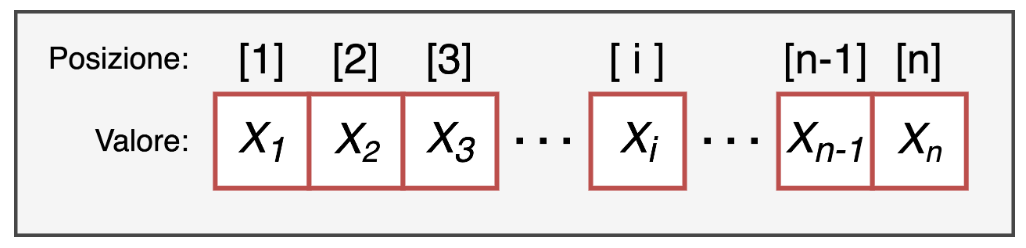
\includegraphics[keepaspectratio]{slides/modulo1/img/vettore.png}}
\end{center}

\textbf{Caratteristiche}:

\begin{itemize}
\item
  \textbf{la lunghezza}: il numero di elementi da cui è formato il
  vettore. La funzione \texttt{length(x)} permette di ottenere la
  lunghezza del vettore x, ovvero permette di conoscere il numero di
  elementi di cui è composto il vettore.
\item
  \textbf{la tipologia}: la tipologia di dati da cui è formato il
  vettore. Un vettore infatti deve esssere formato da \textbf{elementi
  tutti dello stesso tipo} (vedi Section~\ref{sec-vec})!
\end{itemize}

I vettori sono caratterizzati da:

\begin{itemize}
\item
  \textbf{un valore}: il valore dell'elemento che può essere di
  qualsiasi tipo ad esempio un numero o una serie di caratteri.
\item
  \textbf{un indice di posizione}: un numero intero positivo che
  identifica la sua posizione all'interno del vettore.
\end{itemize}

\subsection{\texorpdfstring{Creare un vettore con
\texttt{c()}}{Creare un vettore con c()}}\label{creare-un-vettore-con-c}

Concatena diversi oggetti insieme per creare un nuovo oggetto unico

\begin{Shaded}
\begin{Highlighting}[]
\NormalTok{x }\OtherTok{=} \FunctionTok{c}\NormalTok{(}\DecValTok{1}\NormalTok{, }\DecValTok{2}\NormalTok{, }\DecValTok{3}\NormalTok{) ; x}
\end{Highlighting}
\end{Shaded}

\begin{verbatim}
[1] 1 2 3
\end{verbatim}

\begin{Shaded}
\begin{Highlighting}[]
\NormalTok{X }\OtherTok{=} \DecValTok{1}\SpecialCharTok{:}\DecValTok{3}\NormalTok{ ; X}
\end{Highlighting}
\end{Shaded}

\begin{verbatim}
[1] 1 2 3
\end{verbatim}

\begin{Shaded}
\begin{Highlighting}[]
\NormalTok{x }\SpecialCharTok{==}\NormalTok{ X }
\end{Highlighting}
\end{Shaded}

\begin{verbatim}
[1] TRUE TRUE TRUE
\end{verbatim}

\subsection{Tipologie di vettore}\label{sec-vec}

Tipi di oggetti diversi \(\rightarrow\) Tipi di vettori diversi:

\begin{itemize}
\tightlist
\item
  \texttt{num} (\texttt{numeric}): Numeri \texttt{(-0.56,\ 3,\ 4.5)}
\item
  \texttt{logi} (\texttt{logic}): Logico (\texttt{TRUE} vs
  \texttt{FALSE})
\item
  \texttt{chr} (\texttt{character}): characters
  \texttt{("a",\ "b",\ "c")}
\item
  \texttt{factor} (\texttt{factor}): factor con diversi livelli
\end{itemize}

La distinzione più importante è tra vettori di tipo categoriale
(\texttt{chr} e \texttt{factor}) e vettori di tipo numerico
(\texttt{int} e \texttt{num}):

\begin{itemize}
\tightlist
\item
  \texttt{integer} e \texttt{numeric}: Operazioni matematiche E calcolo
  delle frequenze
\item
  \texttt{character} e \texttt{factor}: Calcolo delle frequenze
\end{itemize}

\begin{Shaded}
\begin{Highlighting}[]
\NormalTok{months }\OtherTok{=} \FunctionTok{c}\NormalTok{(}\DecValTok{5}\NormalTok{, }\DecValTok{6}\NormalTok{, }\DecValTok{8}\NormalTok{, }\DecValTok{10}\NormalTok{, }\DecValTok{12}\NormalTok{, }\DecValTok{16}\NormalTok{); months}
\end{Highlighting}
\end{Shaded}

\begin{verbatim}
[1]  5  6  8 10 12 16
\end{verbatim}

\begin{Shaded}
\begin{Highlighting}[]
\NormalTok{weight }\OtherTok{=} \FunctionTok{runif}\NormalTok{(}\DecValTok{6}\NormalTok{, }\DecValTok{3}\NormalTok{, }\DecValTok{18}\NormalTok{) ; weight}
\end{Highlighting}
\end{Shaded}

\begin{verbatim}
[1] 17.872869 11.524579 15.821762 17.481741  6.328398  7.787142
\end{verbatim}

I vettori logici si ottengono testando delle condizioni sulla base dei
valori di altri vettori (Listing~\ref{lst-test}:

\begin{codelisting}

\caption{\label{lst-test}Testa se ci sono valori maggior di 12
all'interno del vettore}

\centering{

\begin{Shaded}
\begin{Highlighting}[]
\NormalTok{months }\SpecialCharTok{\textgreater{}} \DecValTok{12}
\end{Highlighting}
\end{Shaded}

}

\end{codelisting}%

\begin{verbatim}
[1] FALSE FALSE FALSE FALSE FALSE  TRUE
\end{verbatim}

Il vettore logico risultante può essere utilizzato per filtrare i valori
dal vettore orginale (vedi Section~\ref{sec-filterVec}).

La funzione \texttt{rep()} in Listing~\ref{lst-rep} crea un vettore di
tipo character ripetendo i \(K\) valori per \(X\) volte. Nell'esempio in
Listing~\ref{lst-rep}, le categorie \texttt{low}, \texttt{medium},
\texttt{high} vengono ripertute tutte per due volte (argomento
\texttt{each\ =\ 2}).

La funzione \texttt{factor()} forza il vettore ad essere un vettore con
\(K\) categorie e un numero di valori uguale al numero di elementi
dentro il vettore.

\begin{codelisting}

\caption{\label{lst-rep}Creare un vettore di tipo factor usando la
funzione rep}

\centering{

\begin{Shaded}
\begin{Highlighting}[]
\NormalTok{ses }\OtherTok{=} \FunctionTok{factor}\NormalTok{(}\FunctionTok{rep}\NormalTok{(}\FunctionTok{c}\NormalTok{(}\StringTok{"low"}\NormalTok{, }\StringTok{"medium"}\NormalTok{, }\StringTok{"high"}\NormalTok{), }\AttributeTok{each =} \DecValTok{2}\NormalTok{))}
\NormalTok{ses}
\end{Highlighting}
\end{Shaded}

}

\end{codelisting}%

\begin{verbatim}
[1] low    low    medium medium high   high  
Levels: high low medium
\end{verbatim}

L'argomento \texttt{levels} all'interno della funzione \texttt{factor()}
(vedi Listing~\ref{lst-levels}) permette di specificare l'ordine delle
categorie, altrimenti il default di R le mette in ordine alfabetico.

\begin{codelisting}

\caption{\label{lst-levels}Ordinare i livelli della vraibile con levels}

\centering{

\begin{Shaded}
\begin{Highlighting}[]
\NormalTok{ses }\OtherTok{=} \FunctionTok{factor}\NormalTok{(ses, }\AttributeTok{levels =} \FunctionTok{c}\NormalTok{(}\StringTok{"low"}\NormalTok{, }\StringTok{"medium"}\NormalTok{, }\StringTok{"high"}\NormalTok{))}
\end{Highlighting}
\end{Shaded}

}

\end{codelisting}%

\subsection{Indicizzare i vettori}\label{sec-filterVec}

I vttori si indicizzano usando le parentesi quadre:

\texttt{nome\_vettore{[}indice{]}} dove l'indice è la posizione
all'interno del vettore che si vuole ottenere.

In R, la numerazione delle posizioni all'interno del vettore va da 1
alla lunghezza del vettore.

Dato ad esempio il vettore \texttt{nomi} come segue

\begin{Shaded}
\begin{Highlighting}[]
\NormalTok{nomi }\OtherTok{=} \FunctionTok{c}\NormalTok{(}\StringTok{"Pasquale"}\NormalTok{, }\StringTok{"Egidio"}\NormalTok{, }\StringTok{"Debora"}\NormalTok{, }\StringTok{"Luca"}\NormalTok{, }\StringTok{"Andrea"}\NormalTok{)}
\NormalTok{nomi}
\end{Highlighting}
\end{Shaded}

\begin{verbatim}
[1] "Pasquale" "Egidio"   "Debora"   "Luca"     "Andrea"  
\end{verbatim}

Possiamo immaginare ogni nome come occupante di una specifica posizione
all'interno del vettore, come segue:

\begin{table}[h]
\centering
\begin{tabular}{p{2cm}p{2cm}p{2cm}p{2cm}p{2cm}}
\hline
\multicolumn{1}{|c|}{Pasquale} & \multicolumn{1}{|c|}{Egidio}& \multicolumn{1}{|c|}{Debora} & \multicolumn{1}{|c|}{Luca} & \multicolumn{1}{|c|}{Andrea} \\\hline
& & & & \\
\multicolumn{1}{c}{1} & \multicolumn{1}{c}{2}& \multicolumn{1}{c}{3} & \multicolumn{1}{c}{4} & \multicolumn{1}{c}{5}\\
\end{tabular}
\end{table}

Per cui possiamo estrarre i vari nomi facendo riferimento al loro
indice:

\texttt{nomi{[}1{]}} \(\rightarrow\) Pasquale

\texttt{nomi{[}3{]}} \(\rightarrow\) Debora

\texttt{nomi{[}seq(2,\ 5,\ by\ =\ 2){]}} \(\rightarrow\) Egidio, Luca

\begin{tcolorbox}[enhanced jigsaw, toprule=.15mm, left=2mm, leftrule=.75mm, breakable, coltitle=black, title={\texttt{seq(min,\ max,\ by)}}, bottomtitle=1mm, opacitybacktitle=0.6, toptitle=1mm, titlerule=0mm, bottomrule=.15mm, colframe=quarto-callout-note-color-frame, arc=.35mm, rightrule=.15mm, opacityback=0, colbacktitle=quarto-callout-note-color!10!white, colback=white]

Questa funzione genera un vettore partendo da un valore minimo fino a un
valore massimo con uno step incrementale definito dall'utente:

\begin{Shaded}
\begin{Highlighting}[]
\FunctionTok{seq}\NormalTok{(}\DecValTok{1}\NormalTok{,}\DecValTok{5}\NormalTok{, }\AttributeTok{by =} \FloatTok{0.5}\NormalTok{)}
\end{Highlighting}
\end{Shaded}

\begin{verbatim}
[1] 1.0 1.5 2.0 2.5 3.0 3.5 4.0 4.5 5.0
\end{verbatim}

\end{tcolorbox}

L'indicizzazione dei vettori funziona anche su vettori di tipo numerico,
come negli esempi sequenti:

\begin{Shaded}
\begin{Highlighting}[]
\NormalTok{weight[}\DecValTok{2}\NormalTok{] }\CommentTok{\# secondo elemento di weight}
\end{Highlighting}
\end{Shaded}

\begin{verbatim}
[1] 11.52458
\end{verbatim}

\begin{Shaded}
\begin{Highlighting}[]
\NormalTok{(weight[}\DecValTok{6}\NormalTok{] }\OtherTok{=} \FloatTok{15.2}\NormalTok{) }\CommentTok{\# sostituisce il sesto elemento di weight}
\end{Highlighting}
\end{Shaded}

\begin{verbatim}
[1] 15.2
\end{verbatim}

\begin{Shaded}
\begin{Highlighting}[]
\NormalTok{weight[}\FunctionTok{seq}\NormalTok{(}\DecValTok{1}\NormalTok{, }\DecValTok{6}\NormalTok{, }\AttributeTok{by =} \DecValTok{2}\NormalTok{)] }\CommentTok{\# elementi 1, 3, 5}
\end{Highlighting}
\end{Shaded}

\begin{verbatim}
[1] 17.872869 15.821762  6.328398
\end{verbatim}

\begin{Shaded}
\begin{Highlighting}[]
\NormalTok{weight[}\DecValTok{2}\SpecialCharTok{:}\DecValTok{6}\NormalTok{] }\CommentTok{\# elementi dal 2 al 6 (incluso)}
\end{Highlighting}
\end{Shaded}

\begin{verbatim}
[1] 11.524579 15.821762 17.481741  6.328398 15.200000
\end{verbatim}

\begin{Shaded}
\begin{Highlighting}[]
\NormalTok{weight[}\SpecialCharTok{{-}}\DecValTok{2}\NormalTok{] }\CommentTok{\# rimuove il secondo elemento}
\end{Highlighting}
\end{Shaded}

\begin{verbatim}
[1] 17.872869 15.821762 17.481741  6.328398 15.200000
\end{verbatim}

I vettori logici possono essere utilizzati per estrarre dteerminati
valori da un vettore:

\begin{Shaded}
\begin{Highlighting}[]
\NormalTok{weight }\SpecialCharTok{\textgreater{}} \DecValTok{7} 
\end{Highlighting}
\end{Shaded}

\begin{verbatim}
[1]  TRUE  TRUE  TRUE  TRUE FALSE  TRUE
\end{verbatim}

Restituisce un vettore logico dove si \texttt{TRUE} se il valore in
quella posizione è maggiore di 7 e \texttt{FALSE} in ogni altro caso. In
questo caso si hanno valori veri (quindi osservazioni con un valore
magggiore di 7) nelle seguenti posizioni del vettore:

\begin{verbatim}
[1] 1 2 3 4 6
\end{verbatim}

Usando il vettore logico dentro le parentesi quadre, si otterranno
esattamente i valori che occupano quelle posizioni:

\begin{Shaded}
\begin{Highlighting}[]
\NormalTok{weight[weight }\SpecialCharTok{\textgreater{}} \DecValTok{7}\NormalTok{] }\CommentTok{\# solo i valori \textgreater{} di 7}
\end{Highlighting}
\end{Shaded}

\begin{verbatim}
[1] 17.87287 11.52458 15.82176 17.48174 15.20000
\end{verbatim}

\begin{Shaded}
\begin{Highlighting}[]
\NormalTok{weight[weight }\SpecialCharTok{\textgreater{}=} \FloatTok{4.5} \SpecialCharTok{\&}\NormalTok{ weight }\SpecialCharTok{\textless{}} \DecValTok{8}\NormalTok{] }\CommentTok{\# valori compresi tra 4.5 e 8}
\end{Highlighting}
\end{Shaded}

\begin{verbatim}
[1] 6.328398
\end{verbatim}

\section{Matrici}\label{matrici}

Le matrici sono una struttura dati \textbf{bidimensionale}
(caratterizzate da 2 dimensioni, la funzione \textbf{\texttt{dim()}}
permette di sapere da quante righe e da quante colonne è composta) dove
il numero di righe rappresenta la dimensione 1 e il numero di colonne la
dimensione 2.

\begin{Shaded}
\begin{Highlighting}[]
\NormalTok{my\_mat }\OtherTok{=} \FunctionTok{matrix}\NormalTok{(}\AttributeTok{data =} \DecValTok{1}\SpecialCharTok{:}\DecValTok{10}\NormalTok{, }\AttributeTok{nrow =} \DecValTok{2}\NormalTok{, }\AttributeTok{ncol =} \DecValTok{5}\NormalTok{)}
\NormalTok{my\_mat}
\end{Highlighting}
\end{Shaded}

\begin{verbatim}
     [,1] [,2] [,3] [,4] [,5]
[1,]    1    3    5    7    9
[2,]    2    4    6    8   10
\end{verbatim}

Per creare una matrice in R si può usare la funzione \texttt{matrix()},
come segue

\begin{verbatim}
 `matrix(data, nrow, ncol, byrow = FALSE)`
 
\end{verbatim}

dove \texttt{data} sono i valori che si vogliono mettere all'interno
della matrice, \texttt{nrow} e \texttt{ncol} specificano il numero di
righe e di colonne che si vogliono mettere nella matrice e
\texttt{byrow\ =\ FALSE} (default) indica che i dati vengono organizzati
per colonna (ovvero la matrice viene rimpita seguendo le colonne).

\begin{Shaded}
\begin{Highlighting}[]
\CommentTok{\# crea una matrice con 3 righe e 4 colonne }
\CommentTok{\# (i valori sono sistemati per riga)}
\NormalTok{A }\OtherTok{=} \FunctionTok{matrix}\NormalTok{(}\DecValTok{1}\SpecialCharTok{:}\DecValTok{12}\NormalTok{, }\AttributeTok{nrow=}\DecValTok{3}\NormalTok{, }\AttributeTok{ncol =} \DecValTok{4}\NormalTok{, }\AttributeTok{byrow =} \ConstantTok{TRUE}\NormalTok{)}
\CommentTok{\# assegna dei nomi alle righe }
\FunctionTok{rownames}\NormalTok{(A) }\OtherTok{=} \FunctionTok{paste}\NormalTok{(}\StringTok{"a"}\NormalTok{,}\DecValTok{1}\SpecialCharTok{:}\FunctionTok{nrow}\NormalTok{(A), }\AttributeTok{sep =}\StringTok{"\_"}\NormalTok{) }
\CommentTok{\# assegna dei nomi alle colonne}
\FunctionTok{colnames}\NormalTok{(A) }\OtherTok{=} \FunctionTok{paste}\NormalTok{(}\StringTok{"b"}\NormalTok{,}\DecValTok{1}\SpecialCharTok{:}\FunctionTok{ncol}\NormalTok{(A), }\AttributeTok{sep =}\StringTok{"\_"}\NormalTok{)}
\NormalTok{A}
\end{Highlighting}
\end{Shaded}

\begin{verbatim}
    b_1 b_2 b_3 b_4
a_1   1   2   3   4
a_2   5   6   7   8
a_3   9  10  11  12
\end{verbatim}

Nel caso precedente, la lunghezza del vettore organizzato nella matrice
rientrava perfettamente nel numero di celle disponibili all'interno
della matrice stessa. Se questo non succede, si hanno due casi:

\begin{tcolorbox}[enhanced jigsaw, toprule=.15mm, left=2mm, leftrule=.75mm, breakable, coltitle=black, title={Il numero di celle è un moltiplicando/dividendo della lunghezza del
vettore}, bottomtitle=1mm, opacitybacktitle=0.6, toptitle=1mm, titlerule=0mm, bottomrule=.15mm, colframe=quarto-callout-note-color-frame, arc=.35mm, rightrule=.15mm, opacityback=0, colbacktitle=quarto-callout-note-color!10!white, colback=white]

\begin{Shaded}
\begin{Highlighting}[]
\NormalTok{data }\OtherTok{=} \DecValTok{1}\SpecialCharTok{:}\DecValTok{12}
\FunctionTok{matrix}\NormalTok{(data, }\AttributeTok{nrow =} \DecValTok{6}\NormalTok{, }\AttributeTok{ncol =}\DecValTok{4}\NormalTok{)}
\end{Highlighting}
\end{Shaded}

\begin{verbatim}
     [,1] [,2] [,3] [,4]
[1,]    1    7    1    7
[2,]    2    8    2    8
[3,]    3    9    3    9
[4,]    4   10    4   10
[5,]    5   11    5   11
[6,]    6   12    6   12
\end{verbatim}

Non succede niente, non appaiono warning e la matrice viene creata
ripetendo due volte il vettore originale.

\end{tcolorbox}

\begin{tcolorbox}[enhanced jigsaw, toprule=.15mm, left=2mm, leftrule=.75mm, breakable, coltitle=black, title={Il numero di celle NON è un moltiplicando della lunghezza del vettore}, bottomtitle=1mm, opacitybacktitle=0.6, toptitle=1mm, titlerule=0mm, bottomrule=.15mm, colframe=quarto-callout-note-color-frame, arc=.35mm, rightrule=.15mm, opacityback=0, colbacktitle=quarto-callout-note-color!10!white, colback=white]

\begin{Shaded}
\begin{Highlighting}[]
\NormalTok{data }\OtherTok{=} \DecValTok{1}\SpecialCharTok{:}\DecValTok{12}
\FunctionTok{matrix}\NormalTok{(data, }\AttributeTok{nrow =} \DecValTok{3}\NormalTok{, }\AttributeTok{ncol =}\DecValTok{2}\NormalTok{)}
\end{Highlighting}
\end{Shaded}

\begin{verbatim}
Warning in matrix(data, nrow = 3, ncol = 2): data length differs from size of
matrix: [12 != 3 x 2]
\end{verbatim}

\begin{verbatim}
     [,1] [,2]
[1,]    1    4
[2,]    2    5
[3,]    3    6
\end{verbatim}

Si ottiene un warning, ma R comunque crea la matrice come può.

\end{tcolorbox}

\subsection{Caratteristiche}\label{caratteristiche}

Le matrici di fatto sono la concatenazione bidimensionale di una serie
di vettori. Di conseguenza:

\begin{itemize}
\tightlist
\item
  Possono contenere una sola tipologia di dati
\item
  Essendo bidimensionali, sono necessari due indici di posizione (righe
  e colonne) per identificare un elemento
\item
  Possono essere viste come un insieme di singoli vettori
\end{itemize}

\subsection{Indicizzare le matrici}\label{indicizzare-le-matrici}

La logica per l'indicizzaizone è la stessa che si usa per i vettori,
solo che all'interno delle parentesi quadre va inserito anche l'indice
per le colonne:

\texttt{my\_matrix{[}righe,\ colonne{]}}

Il primo indice fa sempre riferimento alle righe, il secondo alle
colonne:

\begin{longtable}[]{@{}lccc@{}}
\caption{Struttura di una matrice}\tabularnewline
\toprule\noalign{}
& {[},1{]} & {[},2{]} & {[},3{]} \\
\midrule\noalign{}
\endfirsthead
\toprule\noalign{}
& {[},1{]} & {[},2{]} & {[},3{]} \\
\midrule\noalign{}
\endhead
\bottomrule\noalign{}
\endlastfoot
{[}1,{]} & \([1, 1]\) & \([1, 2]\) & \([1, 3]\) \\
{[}2,{]} & \([2, 1]\) & \([2, 2]\) & \([2, 3]\) \\
{[}3,{]} & \([3, 1]\) & \([3, 2]\) & \([3, 3]\) \\
\end{longtable}

Ad esempio, data la matrice \texttt{A}:

\begin{Shaded}
\begin{Highlighting}[]
\NormalTok{A}
\end{Highlighting}
\end{Shaded}

\begin{verbatim}
    b_1 b_2 b_3 b_4
a_1   1   2   3   4
a_2   5   6   7   8
a_3   9  10  11  12
\end{verbatim}

\texttt{A{[}1,\ {]}} \(\rightarrow\) 1, 2, 3, 4

\texttt{A{[},\ 2{]}} \(\rightarrow\) 2, 6, 10

\texttt{A{[}2,\ 3{]}} \(\rightarrow\) 7

\section{Dataframe}\label{dataframe}

Il dataframe è la struttura più ``complessa'', utile e potente di R e
come le matrici, è composto da due dimensioni (righe \(\times\)
colonne).

A differenza delle matrici, può contenere dati di tipo diverso:

\begin{itemize}
\item
  Ogni elemento (colonna) è un vettore con un nome associato
\item
  Ogni colonna deve avere lo stesso numero di elementi di conseguenza
  ogni riga ha lo stesso numero di elementi (struttura rettangolare).
\item
  \textbf{Tutte le colonne (quindi tutti i vettori contenuti nel
  dataframe) devono avere la stessa lunghezza}

  data.frame(. . .)
\end{itemize}

\begin{Shaded}
\begin{Highlighting}[]
\NormalTok{sesso }\OtherTok{=} \FunctionTok{c}\NormalTok{(}\FunctionTok{rep}\NormalTok{(}\FunctionTok{c}\NormalTok{(}\StringTok{"M"}\NormalTok{,}\StringTok{"F"}\NormalTok{), }\AttributeTok{length=}\FunctionTok{length}\NormalTok{(weight)))}
\NormalTok{data }\OtherTok{=} \FunctionTok{data.frame}\NormalTok{(}\AttributeTok{id =} \FunctionTok{paste0}\NormalTok{(}\StringTok{"id"}\NormalTok{, }\DecValTok{1}\SpecialCharTok{:}\FunctionTok{length}\NormalTok{(weight)), }
\NormalTok{                  weight, sesso)}
\NormalTok{data}
\end{Highlighting}
\end{Shaded}

\begin{verbatim}
   id    weight sesso
1 id1 17.872869     M
2 id2 11.524579     F
3 id3 15.821762     M
4 id4 17.481741     F
5 id5  6.328398     M
6 id6 15.200000     F
\end{verbatim}

Per convenzione, i dati sperimentali vengono organizzati in modo che le
unità statistiche siano sulle righe e le variabili sulle colonne. In
questo modo, sapendo il numero di righe si può ricavare il numero di
unità statistiche, sapendo il numero di righe si può ricavare il numero
di variabili misurate su quelle unità statistiche.

\subsection{Indicizzare i dataframe}\label{sec-indDataframe}

I dataframe si possono indicizzar come le matrici utilizzando le
parentesi quadre e i rispettivi indici di riga e colonna:

\begin{verbatim}
data[r, c]
\end{verbatim}

Si può anche usare un'indicizzazione basata sull'estrazione delle
singole colonne con l'operatore \texttt{\$}:

\begin{verbatim}
data$nome_variabile
\end{verbatim}

\begin{Shaded}
\begin{Highlighting}[]
\NormalTok{data}
\end{Highlighting}
\end{Shaded}

\begin{verbatim}
   id    weight sesso
1 id1 17.872869     M
2 id2 11.524579     F
3 id3 15.821762     M
4 id4 17.481741     F
5 id5  6.328398     M
6 id6 15.200000     F
\end{verbatim}

\begin{Shaded}
\begin{Highlighting}[]
\NormalTok{data[}\DecValTok{2}\NormalTok{, }\DecValTok{1}\NormalTok{]}
\end{Highlighting}
\end{Shaded}

\begin{verbatim}
[1] "id2"
\end{verbatim}

\begin{Shaded}
\begin{Highlighting}[]
\NormalTok{data}\SpecialCharTok{$}\NormalTok{weight}
\end{Highlighting}
\end{Shaded}

\begin{verbatim}
[1] 17.872869 11.524579 15.821762 17.481741  6.328398 15.200000
\end{verbatim}

\begin{Shaded}
\begin{Highlighting}[]
\NormalTok{data}\SpecialCharTok{$}\NormalTok{weight[}\DecValTok{2}\NormalTok{]}
\end{Highlighting}
\end{Shaded}

\begin{verbatim}
[1] 11.52458
\end{verbatim}

La stessa logica con cui dai vettori si estraggono tutte le osservazioni
che soddisfano un determinato requisito

\begin{Shaded}
\begin{Highlighting}[]
\NormalTok{weight[weight }\SpecialCharTok{\textgreater{}=} \DecValTok{7}\NormalTok{]}
\end{Highlighting}
\end{Shaded}

\begin{verbatim}
[1] 17.87287 11.52458 15.82176 17.48174 15.20000
\end{verbatim}

Nel caso del dataframe:

Estrae tutte le righe che soddisfano la condizione e tutte le colonne.

\begin{Shaded}
\begin{Highlighting}[]
\NormalTok{data[data}\SpecialCharTok{$}\NormalTok{weight }\SpecialCharTok{\textgreater{}=}\DecValTok{7}\NormalTok{, ]}
\end{Highlighting}
\end{Shaded}

\begin{verbatim}
   id   weight sesso
1 id1 17.87287     M
2 id2 11.52458     F
3 id3 15.82176     M
4 id4 17.48174     F
6 id6 15.20000     F
\end{verbatim}

Estrare i valori del vettore \texttt{data\$id} che soddisfano la
condizione sulla variabile weight.

\begin{Shaded}
\begin{Highlighting}[]
\NormalTok{data}\SpecialCharTok{$}\NormalTok{id[data}\SpecialCharTok{$}\NormalTok{weight }\SpecialCharTok{\textgreater{}=}\DecValTok{7} \SpecialCharTok{\&}\NormalTok{ data}\SpecialCharTok{$}\NormalTok{weight }\SpecialCharTok{\textless{}} \DecValTok{9}\NormalTok{]}
\end{Highlighting}
\end{Shaded}

\begin{verbatim}
character(0)
\end{verbatim}

\subsection{Attributi e
caratteristiche}\label{attributi-e-caratteristiche}

Le funzioni \textbf{\texttt{names()}} , \textbf{\texttt{dim()}},
\textbf{\texttt{nrow()}}, \textbf{\texttt{ncol()}} sono alcune delle
funzioni per ottenere informazioni sulle caratteristiche del dataframe.

La funzione più utile è \textbf{\texttt{str()}} poichè ci restituisce
una veloce overview della struttura del dataframe: dimensioni, tipi di
variabili.

\begin{Shaded}
\begin{Highlighting}[]
\FunctionTok{names}\NormalTok{(data) }\CommentTok{\# estrae i nomi del dataset}
\end{Highlighting}
\end{Shaded}

\begin{verbatim}
[1] "id"     "weight" "sesso" 
\end{verbatim}

\begin{Shaded}
\begin{Highlighting}[]
\FunctionTok{dim}\NormalTok{(data) }\CommentTok{\# numero di righe e numero di colonne del dataset}
\end{Highlighting}
\end{Shaded}

\begin{verbatim}
[1] 6 3
\end{verbatim}

\begin{Shaded}
\begin{Highlighting}[]
\FunctionTok{str}\NormalTok{(data) }\CommentTok{\# restituisce la struttura }
\end{Highlighting}
\end{Shaded}

\begin{verbatim}
'data.frame':   6 obs. of  3 variables:
 $ id    : chr  "id1" "id2" "id3" "id4" ...
 $ weight: num  17.87 11.52 15.82 17.48 6.33 ...
 $ sesso : chr  "M" "F" "M" "F" ...
\end{verbatim}

\begin{Shaded}
\begin{Highlighting}[]
\FunctionTok{nrow}\NormalTok{(data) }\CommentTok{\# numero di righe (equivale al numero di unità statistiche)}
\end{Highlighting}
\end{Shaded}

\begin{verbatim}
[1] 6
\end{verbatim}

\begin{Shaded}
\begin{Highlighting}[]
\FunctionTok{ncol}\NormalTok{(data) }\CommentTok{\# numero di colonne (equivale al numero di variabili)}
\end{Highlighting}
\end{Shaded}

\begin{verbatim}
[1] 3
\end{verbatim}

\begin{tcolorbox}[enhanced jigsaw, toprule=.15mm, left=2mm, leftrule=.75mm, breakable, coltitle=black, title={NB}, bottomtitle=1mm, opacitybacktitle=0.6, toptitle=1mm, titlerule=0mm, bottomrule=.15mm, colframe=quarto-callout-note-color-frame, arc=.35mm, rightrule=.15mm, opacityback=0, colbacktitle=quarto-callout-note-color!10!white, colback=white]

La funzione \textbf{\texttt{str()}} funziona su tutti gli oggetti di R
(vettori, matrici, dataframe, liste).

Restituisce sempre le informazioni circa la dimensionalità e il numero
(e tipo) di elementi contentui nell'oggetto.

\end{tcolorbox}

\section{Liste}\label{liste}

\begin{verbatim}
  list(name1 = obj1, name2 = obj2, name3 = obj3, . . .)
  
\end{verbatim}

Permette di creare liste di oggetti diversi (matrici, vettori, variabli)
di diverso tipo (\texttt{numeric}, \texttt{character},
\texttt{integer}). Ogni oggetto nella lista può avere un nome diverso
che può essere utilizzato per l'indicizzazione (vedi
Section~\ref{sec-indListe}).

Molti dei risultati ottenuti con le funzioni per le analisi statistiche
sono organizzati in liste, proprio perché permettono di contenere
oggetti di natura diversa e con dimensionalità diversa.

\begin{codelisting}

\caption{\label{lst-list}Crea una lista con oggetti diversi (vettori e
matrici). Ad ogni oggetto viene assegnato un nome}

\centering{

\begin{Shaded}
\begin{Highlighting}[]
\NormalTok{A }\OtherTok{\textless{}{-}} \FunctionTok{c}\NormalTok{(}\DecValTok{1}\NormalTok{,}\DecValTok{8}\NormalTok{,}\DecValTok{5}\NormalTok{,}\DecValTok{0}\NormalTok{)}
\NormalTok{M }\OtherTok{\textless{}{-}} \FunctionTok{matrix}\NormalTok{(A, }\DecValTok{2}\NormalTok{, }\DecValTok{2}\NormalTok{)}
\NormalTok{Nomi3 }\OtherTok{\textless{}{-}} \FunctionTok{c}\NormalTok{(}\StringTok{"giorgio"}\NormalTok{, }\StringTok{"ugo"}\NormalTok{, }\StringTok{"anna"}\NormalTok{)}
\NormalTok{LV }\OtherTok{\textless{}{-}} \FunctionTok{c}\NormalTok{(}\ConstantTok{TRUE}\NormalTok{, }\ConstantTok{FALSE}\NormalTok{, }\ConstantTok{TRUE}\NormalTok{, }\ConstantTok{TRUE}\NormalTok{)}
\NormalTok{OgLista }\OtherTok{\textless{}{-}} \FunctionTok{list}\NormalTok{(}\AttributeTok{a =}\NormalTok{ A, }\AttributeTok{Mat =}\NormalTok{ M, }\AttributeTok{nomi =}\NormalTok{ Nomi3, }\AttributeTok{X =}\NormalTok{ LV)}
\FunctionTok{str}\NormalTok{(OgLista)}
\end{Highlighting}
\end{Shaded}

}

\end{codelisting}%

\begin{verbatim}
List of 4
 $ a   : num [1:4] 1 8 5 0
 $ Mat : num [1:2, 1:2] 1 8 5 0
 $ nomi: chr [1:3] "giorgio" "ugo" "anna"
 $ X   : logi [1:4] TRUE FALSE TRUE TRUE
\end{verbatim}

\subsection{Indicizzare le liste}\label{sec-indListe}

\begin{verbatim}
lista[[i]]
\end{verbatim}

\texttt{{[}{[}i{]}{]}}: indice \(i\) dell'i-esimo oggetto all'interno
della lista a cui si vuole accedere (vedi Listing~\ref{lst-indList1})

\begin{codelisting}

\caption{\label{lst-indList1}Accede al secondo oggetto della lista con
il suo indice}

\centering{

\begin{Shaded}
\begin{Highlighting}[]
\NormalTok{OgLista[[}\DecValTok{2}\NormalTok{]]}
\end{Highlighting}
\end{Shaded}

}

\end{codelisting}%

\begin{verbatim}
     [,1] [,2]
[1,]    1    5
[2,]    8    0
\end{verbatim}

\texttt{lista\$nome\_oggetto}

Gli oggetti dentro le liste si possono indicizzare anche attraverso i
loro nomi usando l'operatore \texttt{\$} (vedi
Listing~\ref{lst-indList2}):

\begin{codelisting}

\caption{\label{lst-indList2}Accede al'oggetto Mat nella lista usando il
suo nome}

\centering{

\begin{Shaded}
\begin{Highlighting}[]
\NormalTok{OgLista}\SpecialCharTok{$}\NormalTok{Mat}
\end{Highlighting}
\end{Shaded}

}

\end{codelisting}%

\begin{verbatim}
     [,1] [,2]
[1,]    1    5
[2,]    8    0
\end{verbatim}

\section{Importare dati esterni}\label{importare-dati-esterni}

\subsection{Importa base}\label{importa-base}

\begin{verbatim}
read.csv2("file_path", header = TRUE, sep = ";")
\end{verbatim}

Il default della funzione prevede che la prima riga contenga i nomi
delle variabili (\texttt{header\ =\ TRUE}) e che il separatore di
colonne (ovvero il valore che fa riconoscere ad R le diverse colonne del
dataset) sia ``;'' (\texttt{sep\ =\ ";"}).

Se si possiede un dataset chiamato ``dati'' nella cartella ``data'',
questo codice lo importerà all'interno dell'ambiente.

\begin{Shaded}
\begin{Highlighting}[]
\CommentTok{\# Lettura file dati esterni}
\NormalTok{data }\OtherTok{\textless{}{-}} \FunctionTok{read.csv2}\NormalTok{(}\StringTok{"data/dati.csv"}\NormalTok{)}
\end{Highlighting}
\end{Shaded}

\begin{tcolorbox}[enhanced jigsaw, toprule=.15mm, left=2mm, leftrule=.75mm, breakable, coltitle=black, title={Caution}, bottomtitle=1mm, opacitybacktitle=0.6, toptitle=1mm, titlerule=0mm, bottomrule=.15mm, colframe=quarto-callout-caution-color-frame, arc=.35mm, rightrule=.15mm, opacityback=0, colbacktitle=quarto-callout-caution-color!10!white, colback=white]

Nei dataset messi a disposizione per questo corso, si deve sempre usare
la funzione \texttt{read.csv2()}.

Perché il codice di sopra funzioni, si assume che la cartella
\texttt{data} sia all'interno del progetto R creato per il corso (vedi
Section~\ref{sec-project}).

\end{tcolorbox}

\subsection{Importa alternativa 1}\label{importa-alternativa-1}

\begin{tcolorbox}[enhanced jigsaw, toprule=.15mm, left=2mm, leftrule=.75mm, breakable, coltitle=black, title={Warning}, bottomtitle=1mm, opacitybacktitle=0.6, toptitle=1mm, titlerule=0mm, bottomrule=.15mm, colframe=quarto-callout-warning-color-frame, arc=.35mm, rightrule=.15mm, opacityback=0, colbacktitle=quarto-callout-warning-color!10!white, colback=white]

Questa alternativa è presentata solo per completezza di informazione, ma
è fortemente sconsigliata visto che non può essere automatizzata dentro
i documento quarto.

\end{tcolorbox}

\begin{center}
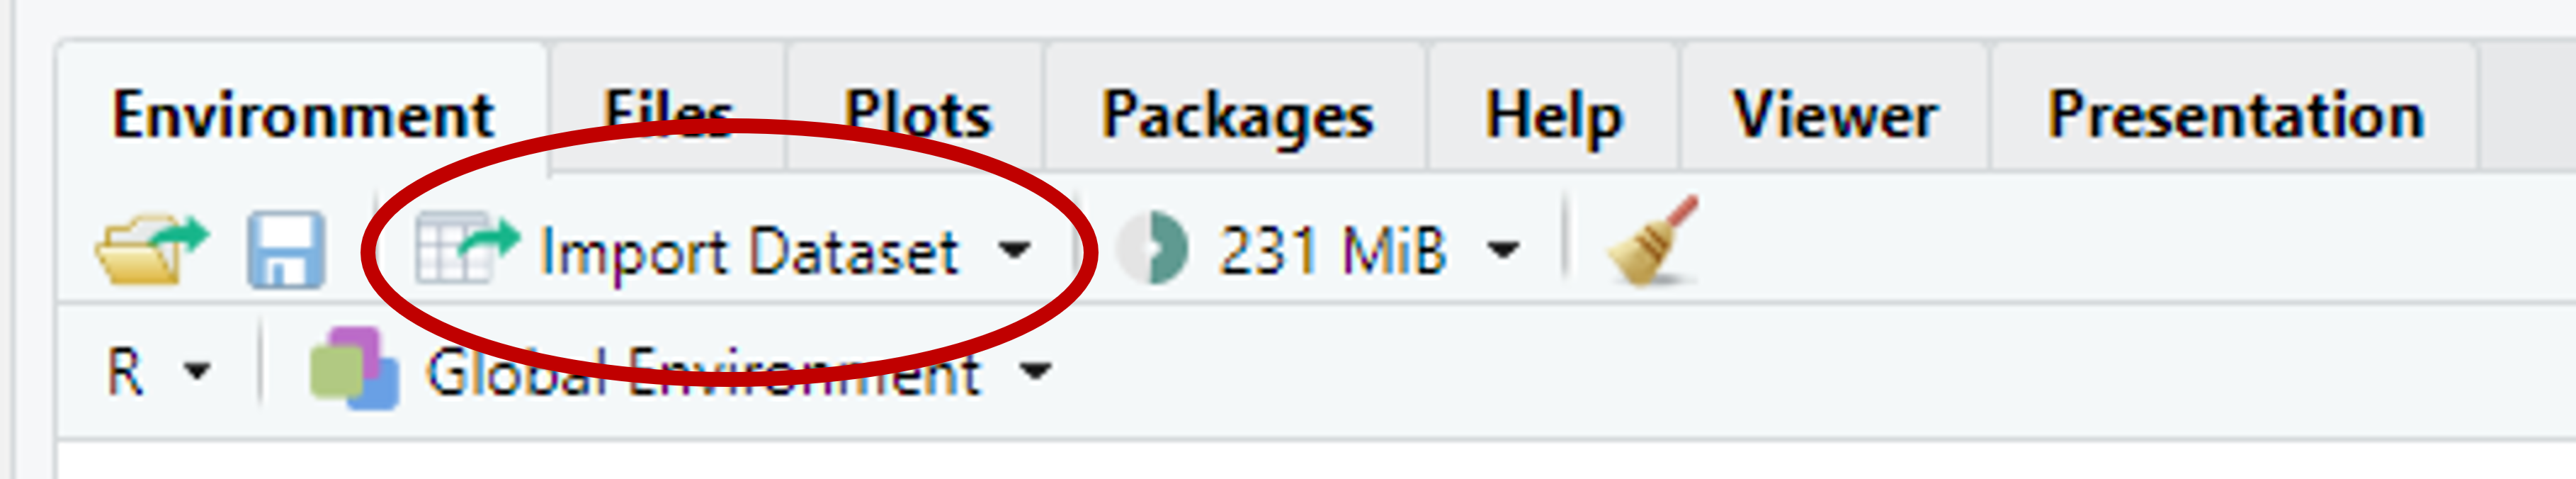
\includegraphics[width=1\linewidth,height=\textheight,keepaspectratio]{slides/modulo1/img/import0.png}
\end{center}

\begin{center}
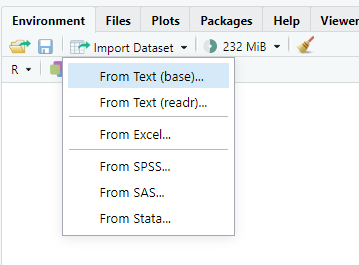
\includegraphics[width=1\linewidth,height=\textheight,keepaspectratio]{slides/modulo1/img/import1.png}
\end{center}

\begin{center}
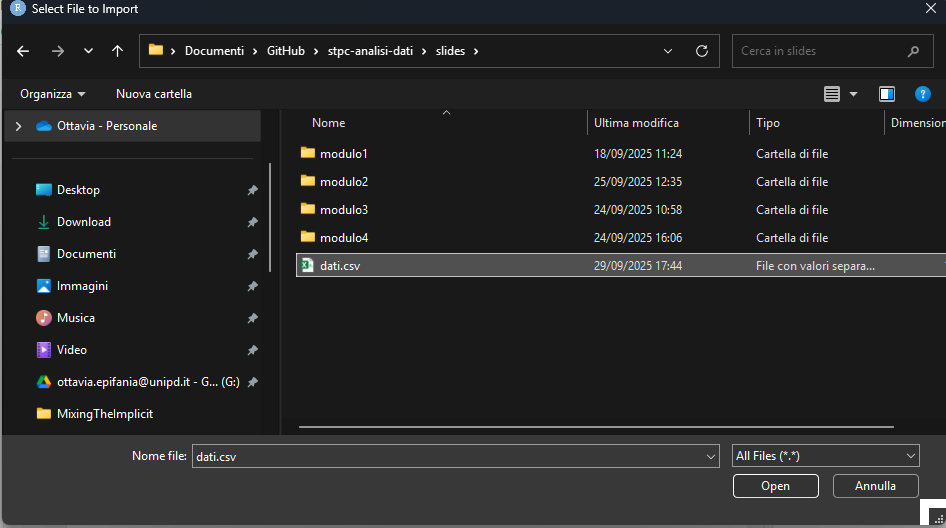
\includegraphics[width=1\linewidth,height=\textheight,keepaspectratio]{slides/modulo1/img/import2.png}
\end{center}

\begin{center}
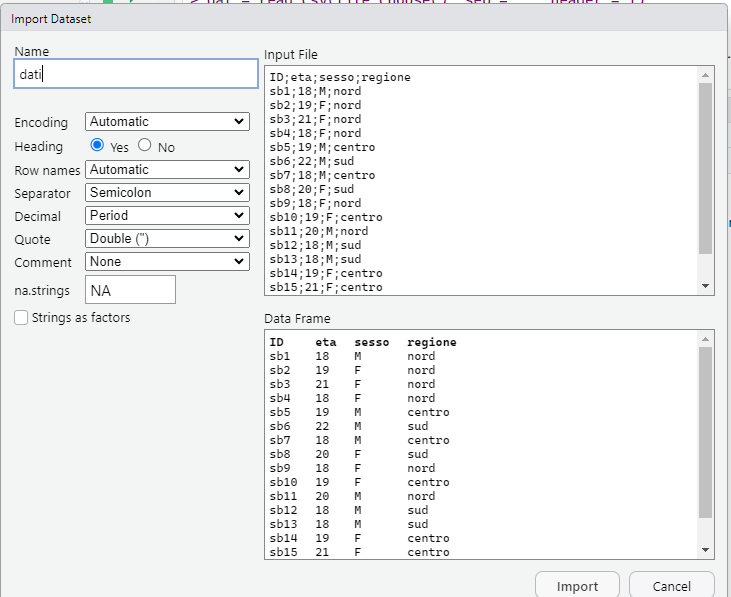
\includegraphics[width=1\linewidth,height=\textheight,keepaspectratio]{slides/modulo1/img/import3.png}
\end{center}

\subsection{Importa alternativa 2}\label{importa-alternativa-2}

\begin{tcolorbox}[enhanced jigsaw, toprule=.15mm, left=2mm, leftrule=.75mm, breakable, coltitle=black, title={Warning}, bottomtitle=1mm, opacitybacktitle=0.6, toptitle=1mm, titlerule=0mm, bottomrule=.15mm, colframe=quarto-callout-warning-color-frame, arc=.35mm, rightrule=.15mm, opacityback=0, colbacktitle=quarto-callout-warning-color!10!white, colback=white]

Questa funzione è la funzione base su cui poggia \texttt{read.csv2()}.
Cambiano i default, che in questo caso sono ottimizzati per i file csv
creati in altre regioni del mondo, dove ``,'' è il sepratore di colonna
di default e ``.'' è il separatore di decimali di default.

\end{tcolorbox}

\begin{Shaded}
\begin{Highlighting}[]
\NormalTok{dati }\OtherTok{=} \FunctionTok{read.csv}\NormalTok{(}\StringTok{"slides/dati.csv"}\NormalTok{, }
                \AttributeTok{sep =}\StringTok{","}\NormalTok{, }\AttributeTok{dec =}\StringTok{"."}\NormalTok{, }\AttributeTok{header =} \ConstantTok{TRUE}\NormalTok{)}
\FunctionTok{head}\NormalTok{(dati)}
\end{Highlighting}
\end{Shaded}

\begin{verbatim}
  ID.eta.sesso.regione
1        sb1;18;M;nord
2        sb2;19;F;nord
3        sb3;21;F;nord
4        sb4;18;F;nord
5      sb5;19;M;centro
6         sb6;22;M;sud
\end{verbatim}

\section{Sintesi delle strutture
tabellari}\label{sintesi-delle-strutture-tabellari}

\subsection{\texorpdfstring{Riassunto descrittivo:
\texttt{summary()}}{Riassunto descrittivo: summary()}}\label{riassunto-descrittivo-summary}

\begin{verbatim}
summary(data)
\end{verbatim}

Riassume il contenuto di strutture di dati, riportando diverse
statistiche descrittive (Table~\ref{tbl-summary}). Tutte le statistiche
descrittive possono essere ottenute con funzioni equivalenti.

\begin{longtable}[]{@{}
  >{\raggedright\arraybackslash}p{(\linewidth - 6\tabcolsep) * \real{0.0755}}
  >{\raggedright\arraybackslash}p{(\linewidth - 6\tabcolsep) * \real{0.1447}}
  >{\raggedright\arraybackslash}p{(\linewidth - 6\tabcolsep) * \real{0.6101}}
  >{\raggedright\arraybackslash}p{(\linewidth - 6\tabcolsep) * \real{0.1698}}@{}}
\caption{Statistiche restituite dalla funzione \texttt{summary()} per
una variabile numerica}\label{tbl-summary}\tabularnewline
\toprule\noalign{}
\begin{minipage}[b]{\linewidth}\raggedright
Statistica
\end{minipage} & \begin{minipage}[b]{\linewidth}\raggedright
Nome
\end{minipage} & \begin{minipage}[b]{\linewidth}\raggedright
Cosa indica
\end{minipage} & \begin{minipage}[b]{\linewidth}\raggedright
Funzione equivalente
\end{minipage} \\
\midrule\noalign{}
\endfirsthead
\toprule\noalign{}
\begin{minipage}[b]{\linewidth}\raggedright
Statistica
\end{minipage} & \begin{minipage}[b]{\linewidth}\raggedright
Nome
\end{minipage} & \begin{minipage}[b]{\linewidth}\raggedright
Cosa indica
\end{minipage} & \begin{minipage}[b]{\linewidth}\raggedright
Funzione equivalente
\end{minipage} \\
\midrule\noalign{}
\endhead
\bottomrule\noalign{}
\endlastfoot
\texttt{Min.} & Minimo & Il valore più piccolo osservato &
\texttt{min(x)} \\
\texttt{1st\ Qu.} & Primo quartile (\(Q_1\)) & Il valore preceduto dal
25\% delle osservazioni e superato dal restante 75\% &
\texttt{quantile(x,\ 0.25)} \\
\texttt{Median} & Mediana (\(Q_2\)) & Il valore centrale della
distribuzione ordinata: il 50\% delle osservazioni sta sotto, il 50\%
sopra & \texttt{median(x)} \\
\texttt{Mean} & Media aritmetica & Il baricentro della distribuzione: la
somma dei valori divisa per il numero di osservazioni &
\texttt{mean(x)} \\
\texttt{3rd\ Qu.} & Terzo quartile (\(Q_3\)) & Il valore preceduto dal
75\% delle osservazioni e superato dal restante 25\% &
\texttt{quantile(x,\ 0.75)} \\
\texttt{Max.} & Massimo & Il valore più grande osservato &
\texttt{max(x)} \\
\texttt{NA\textquotesingle{}s} & Valori mancanti & Il numero di
osservazioni mancanti (compare solo se ce ne sono) &
\texttt{sum(is.na(x))} \\
\end{longtable}

\begin{Shaded}
\begin{Highlighting}[]
\FunctionTok{summary}\NormalTok{(rock)}
\end{Highlighting}
\end{Shaded}

\begin{verbatim}
      area            peri            shape              perm        
 Min.   : 1016   Min.   : 308.6   Min.   :0.09033   Min.   :   6.30  
 1st Qu.: 5305   1st Qu.:1414.9   1st Qu.:0.16226   1st Qu.:  76.45  
 Median : 7487   Median :2536.2   Median :0.19886   Median : 130.50  
 Mean   : 7188   Mean   :2682.2   Mean   :0.21811   Mean   : 415.45  
 3rd Qu.: 8870   3rd Qu.:3989.5   3rd Qu.:0.26267   3rd Qu.: 777.50  
 Max.   :12212   Max.   :4864.2   Max.   :0.46413   Max.   :1300.00  
\end{verbatim}

\subsection{\texorpdfstring{Struttura:
\texttt{str()}}{Struttura: str()}}\label{struttura-str}

\begin{verbatim}
str(data)
\end{verbatim}

Fornisce informazioni circa la struttura generale di un oggetto
(qualsiasi oggetto):

\begin{Shaded}
\begin{Highlighting}[]
\FunctionTok{str}\NormalTok{(rock) }\CommentTok{\#dataframe}
\end{Highlighting}
\end{Shaded}

\begin{verbatim}
'data.frame':   48 obs. of  4 variables:
 $ area : int  4990 7002 7558 7352 7943 7979 9333 8209 8393 6425 ...
 $ peri : num  2792 3893 3931 3869 3949 ...
 $ shape: num  0.0903 0.1486 0.1833 0.1171 0.1224 ...
 $ perm : num  6.3 6.3 6.3 6.3 17.1 17.1 17.1 17.1 119 119 ...
\end{verbatim}

\begin{Shaded}
\begin{Highlighting}[]
\FunctionTok{str}\NormalTok{(weight)}
\end{Highlighting}
\end{Shaded}

\begin{verbatim}
 num [1:6] 17.87 11.52 15.82 17.48 6.33 ...
\end{verbatim}

\subsection{\texorpdfstring{L'inizio \texttt{head()} e la fine
\texttt{tail()} di un
oggetto}{L'inizio head() e la fine tail() di un oggetto}}\label{linizio-head-e-la-fine-tail-di-un-oggetto}

\texttt{head()}

Le prime 6 osservazioni del dataset

\begin{Shaded}
\begin{Highlighting}[]
\FunctionTok{head}\NormalTok{(rock)}
\end{Highlighting}
\end{Shaded}

\begin{verbatim}
  area    peri     shape perm
1 4990 2791.90 0.0903296  6.3
2 7002 3892.60 0.1486220  6.3
3 7558 3930.66 0.1833120  6.3
4 7352 3869.32 0.1170630  6.3
5 7943 3948.54 0.1224170 17.1
6 7979 4010.15 0.1670450 17.1
\end{verbatim}

\texttt{tail()}

le ultime 6 osservazioni del dataset

\begin{Shaded}
\begin{Highlighting}[]
\FunctionTok{tail}\NormalTok{(rock)}
\end{Highlighting}
\end{Shaded}

\begin{verbatim}
   area     peri    shape perm
43 5605 1145.690 0.464125 1300
44 8793 2280.490 0.420477 1300
45 3475 1174.110 0.200744  580
46 1651  597.808 0.262651  580
47 5514 1455.880 0.182453  580
48 9718 1485.580 0.200447  580
\end{verbatim}

\subsection{\texorpdfstring{\texttt{apply()}}{apply()}}\label{apply}

Ci sono diverse funzioni in R che permettono di applicare la stessa
funzione più volte su uno stesso oggetto, come ad esempio la funzione
\texttt{apply()}:

\begin{verbatim}
apply(data, MARGIN, FUN)
\end{verbatim}

\texttt{data}: i dati su cui si vuole lavorare. Si può prendere anche
una sottoselezione di dati utilizzando l'indicizzazione del dataframe
(sia per le righe sia per le colonne, vedi
Section~\ref{sec-indDataframe}).

\texttt{MARGIN\ =\ 1}: applica la funzione sulle righe (attraverso le
colonne). Questo vuol dire che si ottiene un vettore dei risultati di
lunghezza uguale al numero di righe del dataframe.

\texttt{MARGIN\ =\ 2}: applica la funzione sulle colonne (attraverso le
righe). Questo vuol dire che si ottiene un vettore dei risultati di
lunghezza uguale al numero di colonne del dataframe.

\texttt{FUN}: la funzione che si vuole applicare

\begin{Shaded}
\begin{Highlighting}[]
\FunctionTok{apply}\NormalTok{(rock, }\DecValTok{1}\NormalTok{, sum)   }\CommentTok{\# Somma per riga }
\end{Highlighting}
\end{Shaded}

\begin{verbatim}
 [1]  7788.290 10901.049 11495.143 11227.737 11908.762 12006.417 13696.040
 [8] 12571.014 12194.244  9642.812 13963.201 12729.388 14770.169 12468.672
[15] 13498.943 12585.623 15629.464 15589.483 16801.020 14405.155 11408.854
[22] 16371.431 17051.890 11893.602  9077.671  6312.529 10072.432  7571.553
[29]  9250.435  7025.001  9393.452 10245.336  8356.958  7258.715  9692.914
[36] 10305.336  4945.877  2044.761  4813.624  7012.214  7289.872  2624.872
[43]  8051.154 12373.910  5229.311  2829.071  7550.062 11783.780
\end{verbatim}

\begin{Shaded}
\begin{Highlighting}[]
\FunctionTok{apply}\NormalTok{(rock, }\DecValTok{2}\NormalTok{, mean)  }\CommentTok{\# Media per colonna }
\end{Highlighting}
\end{Shaded}

\begin{verbatim}
        area         peri        shape         perm 
7187.7291667 2682.2119375    0.2181104  415.4500000 
\end{verbatim}

\chapter{Modulo 2 -- Scale di misura e statistica descrittiva
univariata}\label{modulo-2-scale-di-misura-e-statistica-descrittiva-univariata}

\section{Tipi di variabili}\label{tipi-di-variabili}

\textbf{QUALITATIVE / CATEGORIALI}

\begin{itemize}
\tightlist
\item
  Sconnesse: \(\{a, b, c\}\)
\item
  Ordinate: \(\{a, b, c\}\) con \(a < b < c\) (oppure \(a > b > c\))
\end{itemize}

\textbf{QUANTITATIVE / METRICHE}

\begin{itemize}
\tightlist
\item
  Discrete: \(\mathbb{Z}\)
\item
  Continue: \(\mathbb{R}\)
\end{itemize}

\section{Scale di misura (Stevens,
1946)}\label{scale-di-misura-stevens-1946}

Le variabili si differenziano in base alla quantità di informazione che
può essere ricavata.

\begin{itemize}
\item Variabili qualitative
\begin{itemize}
\item \textbf{Nominale}: Distingue un insieme di dati in diverse categorie
\item \textbf{Ordinale}: Distingue un insieme di dati in diverse categorie che sono ordinabili a seconda della quantità di caratteristica posseduta 
\end{itemize}
    
\item Variabili quantitative
    
\begin{itemize}
\item \textbf{Intervalli equivalenti} Distingue un insieme di dati in diverse categorie ordinabili. La distanza tra le categorie è nota perché c'è un'unità di misura
\item \textbf{A rapporti equivalenti}: Come la scala ad intervalli...ma lo 0 indica assenza di caratteristica (non è arbitrario ma è assoluto) 
\end{itemize}
\end{itemize}

\subsection{Categoriali - Nominali}\label{categoriali---nominali}

Comune di residenza, sesso biologico, patologia clinica ecc.

\subsubsection{\texorpdfstring{\texttt{as.factor()}}{as.factor()}}\label{as.factor}

\texttt{as.factor()}: Converte una variabile in una variabile di tipo
\textbf{categoriale/nominale} con tanti livelli quanti sono i valori
unici nel vettore

\textbf{Due livelli}

\begin{Shaded}
\begin{Highlighting}[]
\NormalTok{Genere }\OtherTok{\textless{}{-}} \FunctionTok{c}\NormalTok{(}\StringTok{"m"}\NormalTok{,}\StringTok{"f"}\NormalTok{,}\StringTok{"f"}\NormalTok{,}\StringTok{"m"}\NormalTok{,}\StringTok{"f"}\NormalTok{,}\StringTok{"m"}\NormalTok{) }
\NormalTok{Genere}
\end{Highlighting}
\end{Shaded}

\begin{verbatim}
[1] "m" "f" "f" "m" "f" "m"
\end{verbatim}

\begin{Shaded}
\begin{Highlighting}[]
\FunctionTok{as.factor}\NormalTok{(Genere) }
\end{Highlighting}
\end{Shaded}

\begin{verbatim}
[1] m f f m f m
Levels: f m
\end{verbatim}

\texttt{as.character()} produre una variabili categoriale, ma senza i
livelli che caratterizzano i \texttt{factor}

\textbf{Più livelli}

\begin{Shaded}
\begin{Highlighting}[]
\NormalTok{diagnosi }\OtherTok{\textless{}{-}} \FunctionTok{c}\NormalTok{(}\StringTok{"schizo"}\NormalTok{, }\StringTok{"dep"}\NormalTok{, }\StringTok{"narc"}\NormalTok{, }\StringTok{"schizo"}\NormalTok{, }\StringTok{"dep"}\NormalTok{, }\StringTok{"narc"}\NormalTok{)}
\NormalTok{diagnosi}
\end{Highlighting}
\end{Shaded}

\begin{verbatim}
[1] "schizo" "dep"    "narc"   "schizo" "dep"    "narc"  
\end{verbatim}

\begin{Shaded}
\begin{Highlighting}[]
\FunctionTok{as.factor}\NormalTok{(diagnosi) }
\end{Highlighting}
\end{Shaded}

\begin{verbatim}
[1] schizo dep    narc   schizo dep    narc  
Levels: dep narc schizo
\end{verbatim}

\subsection{Scala ordinale}\label{scala-ordinale}

Distingue un insieme di dati in diverse categorie che sono ordinabili a
seconda della quantità di caratteristica posseduta. Vale sia
l'equivalenza (\(=\) o \(\neq\)) sia l'ordinamento (\(<\) o \(>\)).

Esempi: Titolo di studio, gradimento di un prodotto, valutazione di una
malattia (alto, medio, basso).

Le etichette numeriche valgono per il loro ordine (non ha senso compiere
operazioni tra di loro).

\begin{center}
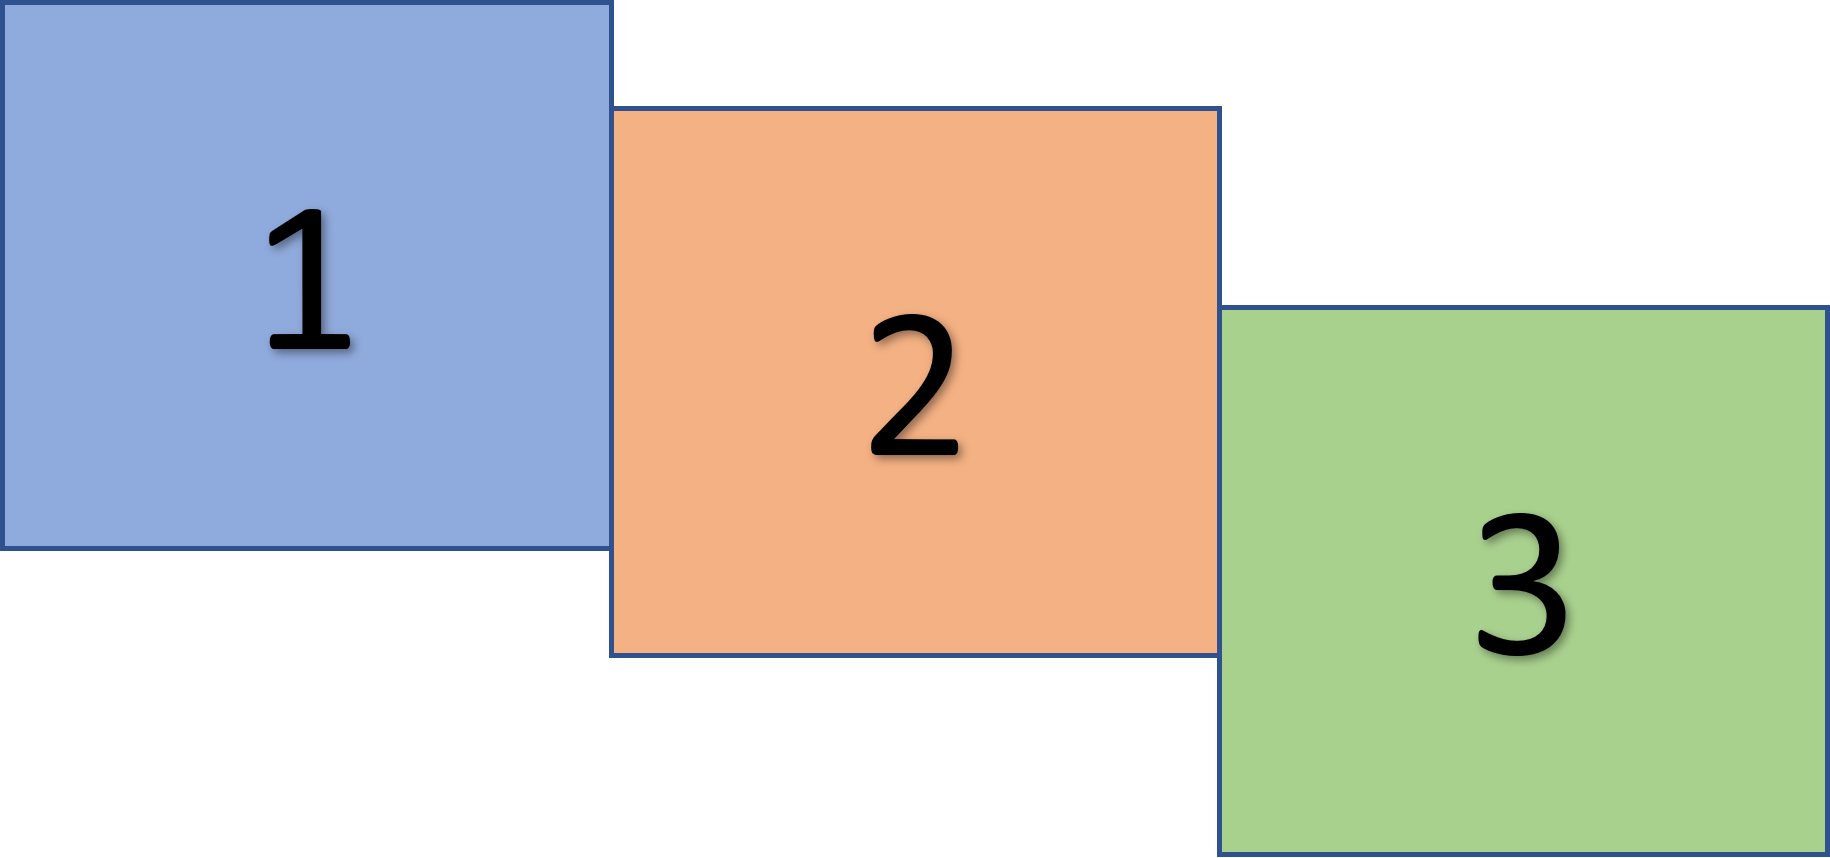
\includegraphics[width=.20\linewidth]{slides/modulo2/img/ordinale.png}
\end{center}

\begin{tcolorbox}[enhanced jigsaw, toprule=.15mm, left=2mm, leftrule=.75mm, breakable, coltitle=black, title={Attenzione!}, bottomtitle=1mm, opacitybacktitle=0.6, toptitle=1mm, titlerule=0mm, bottomrule=.15mm, colframe=quarto-callout-caution-color-frame, arc=.35mm, rightrule=.15mm, opacityback=0, colbacktitle=quarto-callout-caution-color!10!white, colback=white]

Si conosce l'ordine tra le categorie, non si conosce la distanza.

Le etichette numeriche valgono per il loro ordine (non ha senso compiere
operazioni tra di loro)

\end{tcolorbox}

\begin{verbatim}
factor(A,levels=c("a1","a2",..., "ak"), ordered=TRUE) 
   
\end{verbatim}

Converte la variabile in una variabile con tanti livelli quanti sono i
valori unici e viene forzato un ordine su questi livelli:

\begin{codelisting}

\caption{\label{lst-order}Utilizzo dell'agormento levels per ordinare i
livelli di una variabile categoriale ordinata}

\centering{

\begin{Shaded}
\begin{Highlighting}[]
\NormalTok{Voto }\OtherTok{\textless{}{-}} \FunctionTok{c}\NormalTok{(}\StringTok{"alto"}\NormalTok{,}\StringTok{"medio"}\NormalTok{,}\StringTok{"medio"}\NormalTok{,}\StringTok{"basso"}\NormalTok{,}\StringTok{"alto"}\NormalTok{) }
\NormalTok{Voto}
\end{Highlighting}
\end{Shaded}

}

\end{codelisting}%

\begin{verbatim}
[1] "alto"  "medio" "medio" "basso" "alto" 
\end{verbatim}

\begin{codelisting}

\caption{\label{lst-order}Utilizzo dell'agormento levels per ordinare i
livelli di una variabile categoriale ordinata}

\centering{

\begin{Shaded}
\begin{Highlighting}[]
\FunctionTok{factor}\NormalTok{(Voto,}\AttributeTok{levels=}\FunctionTok{c}\NormalTok{(}\StringTok{"basso"}\NormalTok{,}\StringTok{"medio"}\NormalTok{,}\StringTok{"alto"}\NormalTok{)) }
\end{Highlighting}
\end{Shaded}

}

\end{codelisting}%

\begin{verbatim}
[1] alto  medio medio basso alto 
Levels: basso medio alto
\end{verbatim}

\begin{tcolorbox}[enhanced jigsaw, toprule=.15mm, left=2mm, leftrule=.75mm, breakable, coltitle=black, title={Warning}, bottomtitle=1mm, opacitybacktitle=0.6, toptitle=1mm, titlerule=0mm, bottomrule=.15mm, colframe=quarto-callout-warning-color-frame, arc=.35mm, rightrule=.15mm, opacityback=0, colbacktitle=quarto-callout-warning-color!10!white, colback=white]

L'utilizzo dell'argomento ordered è deprecato, sconsiglio di usarlo. In
caso di variabili ordinali, è sufficiente ordinare i livelli attraverso
l'argomento levels come mostrato oin Listing~\ref{lst-order}.

\end{tcolorbox}

\subsection{Scala a intervalli
equivalenti}\label{scala-a-intervalli-equivalenti}

Lo \(0\) è arbitrario, ma c'è un'unità di misura per cui le categorie si
trovano alla stessa distanza. Vale equivalenza (\(=\) o \(\neq\)),
ordinamento (\(<\) o \(>\)) e differenza (\(+\) o \(-\)).

Esiste una relazione d'ordine tra le quantità e la distanza tra le
quantità è nota e definita da una unità di misura costante e
\textbf{nota}.

Esempi: Temperatura in Celsius, Q.I., scale di atteggiamento.

Se ci sono 0°C, non vuol dire che non c'è calore!

Prendiamo due temperature, \(T_a\) e \(T_b\). Queste temperature in
Celsius \(C\) sono \(T_a(C) = 5\) e \(T_b(C) = 10\).

Quello che si può dire:

\begin{itemize}
\tightlist
\item
  \(T_a(C) < T_b(C)\) (oppure \(T_b(C) > T_a(C)\))
\item
  \(T_b(C) - T_a(C) = 5\)
\item
  Non possiamo dire che \(T_b(C) = 2T_a(C)\).
\end{itemize}

Infatti, volendo trasformare le due temperature in Fahrenheit tramite la
relazione:

\[F = \dfrac{9}{5}C + 32\] si vedrebbe che
\(T_a(F) = \dfrac{9}{5}5 + 32 = 41\) e
\(T_a(F) = \dfrac{9}{5}10 + 32 = 50\).

Rimane la relazione d'ordine, per cui anche \(T_a(F) < T_b(F)\), ma
cambia sia la differenza tra le due quantità \(T_b(F) - T_a(F) = 9\) sia
la relazione tra le due, per cui si vede chiaramente che
\(T_a(F) \neq T_b(F)\).

\begin{center}
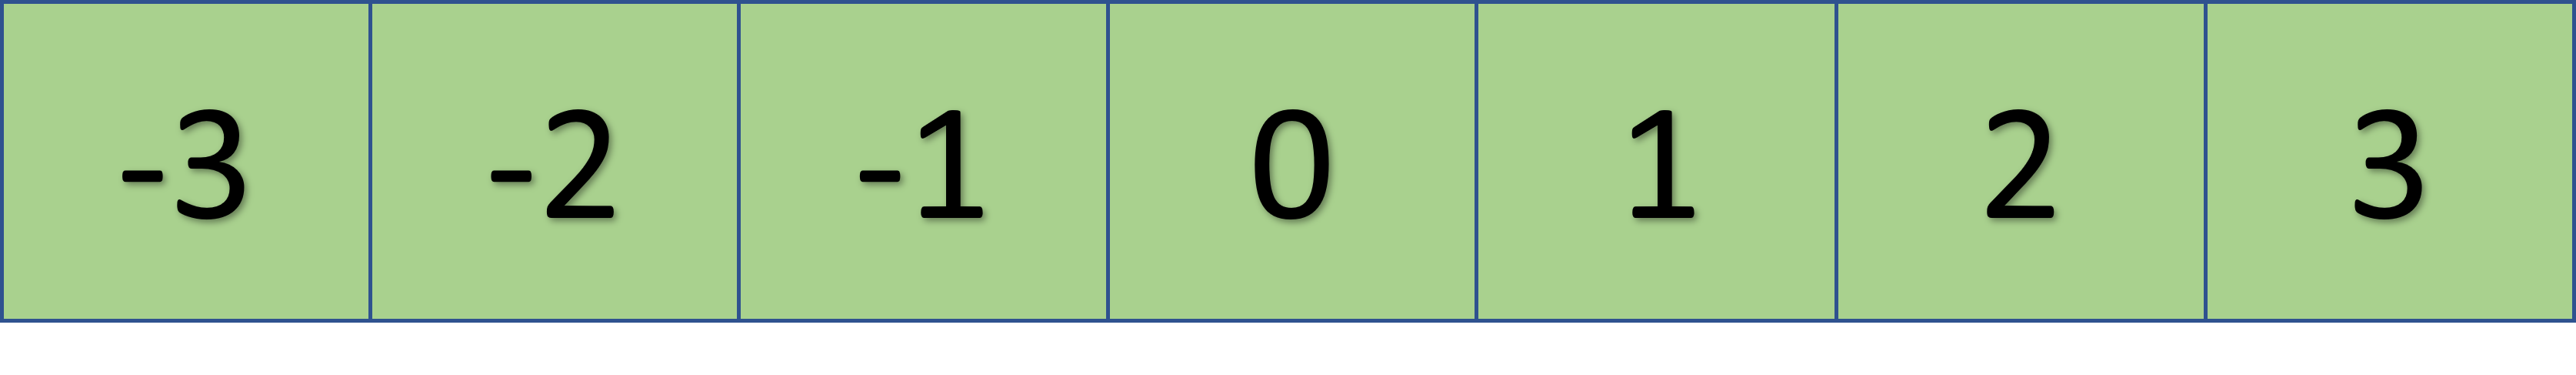
\includegraphics[width=0.5\linewidth]{slides/modulo2/img/intervalli.png}
\end{center}

\begin{center}
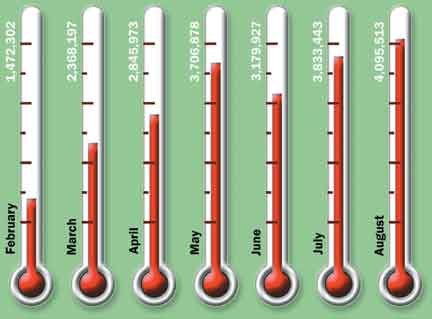
\includegraphics[width=0.5\linewidth]{slides/modulo2/img/termometroMulti.jpg}
\end{center}

\begin{center}
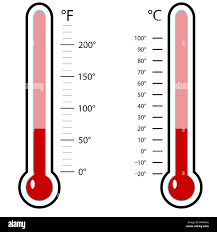
\includegraphics[width=0.3\linewidth]{slides/modulo2/img/termometri}
\end{center}

\subsection{Scala a rapporti
equivalenti}\label{scala-a-rapporti-equivalenti}

Lo \(0\) è assoluto: indica assenza del fenomeno. Vale equivalenza
(\(=\) o \(\neq\)), ordinamento (\(<\) o \(>\)), differenza (\(+\) o
\(-\)) e rapporto (\(\times\) o \(\div\)).

Esempi: Peso, altezza, valori diagnostici.

La presenza dello 0 assoluto permette di andare oltre la mera relazione
d'ordine e distanza tra le quantità.

Si prendano ad esempio due pesi, \(P_a\) e \(P_b\). Questi pesi,
misurati in chilogrammi \(K\), sono \(P_a(K)= 10\) e \(P_b(K) = 30\).
Quello che si può dire:

\begin{itemize}
\tightlist
\item
  \(P_a(K) < P_b(K)\) (\(P_b(K) > P_a(K)\))
\item
  \(P_b(K) - P_a(K) = 20\)
\item
  Ma soprattutto \(P_a(K) = \dfrac{1}{3}P_b(K)\) oppure
  \(P_b(K) = 3P_a(K)\)
\end{itemize}

La relazione tra \(P_a\) e \(P_b\) rimane \textbf{invariante} attraverso
le diverse trasformazioni di scala.

Ad esempio, trasformando \(P_a(K)\) e \(P_b(K)\) in libbre (\(L\))
mediante la relazione

\[L = K \times 2.20462\] per cui
\(P_a(L) = 10 \times 2.20462 = 22.0462\) e
\(P_b(L) = 20 \times 2.20462 = 44.0924\). La relazione d'ordine è
matenuta e, al netto dei decimali, rimane anche invariante il rapporto
tra i due pesi.

\begin{center}
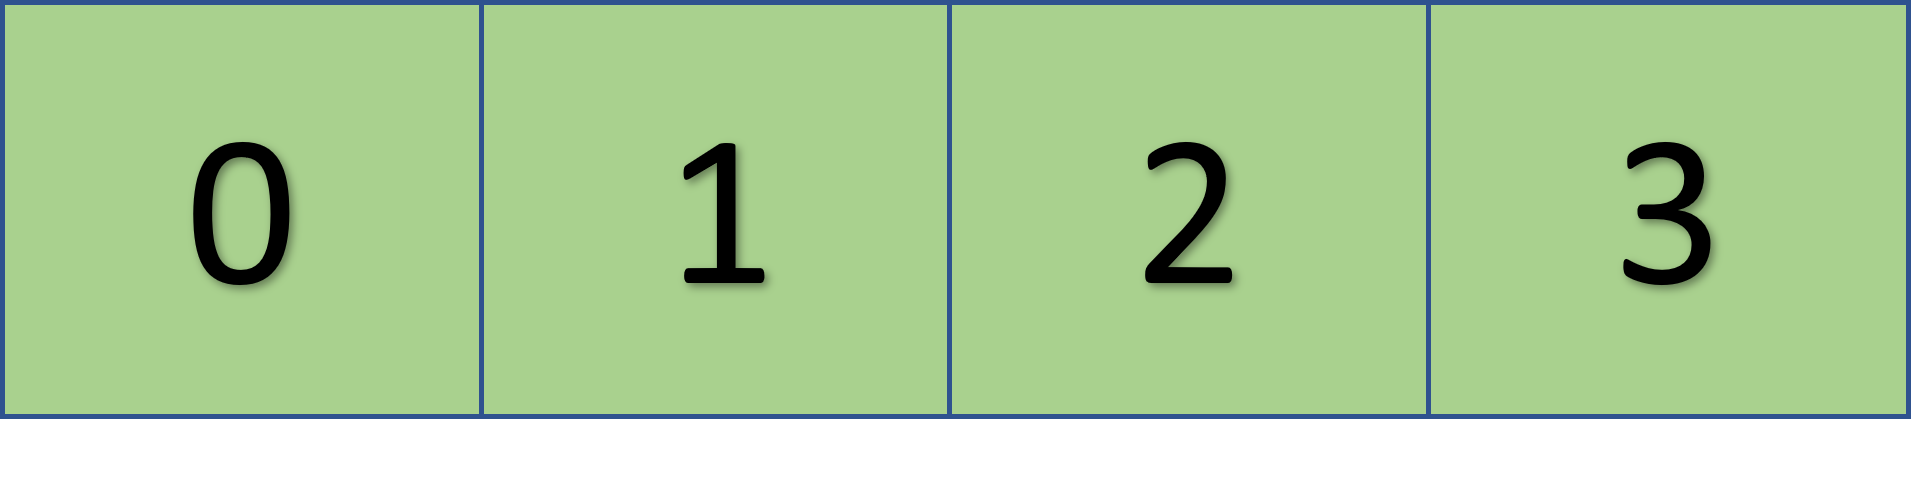
\includegraphics[width=0.40\linewidth]{slides/modulo2/img/rapporti.png}
\end{center}

\begin{center}
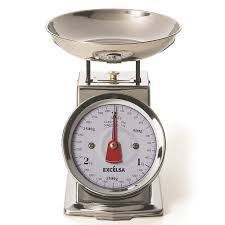
\includegraphics[width=0.4\linewidth]{slides/modulo2/img/bilancia}
\end{center}

\subsubsection{\texorpdfstring{\texttt{numeric},
\texttt{integer()}}{numeric, integer()}}\label{numeric-integer}

Le \textbf{variabili metriche} in R sono variabili di tipo
\texttt{numeric} o \texttt{integer}, a seconda che siano continue o
discrete

\begin{tcolorbox}[enhanced jigsaw, toprule=.15mm, left=2mm, leftrule=.75mm, breakable, coltitle=black, title={Attenzione!}, bottomtitle=1mm, opacitybacktitle=0.6, toptitle=1mm, titlerule=0mm, bottomrule=.15mm, colframe=quarto-callout-caution-color-frame, arc=.35mm, rightrule=.15mm, opacityback=0, colbacktitle=quarto-callout-caution-color!10!white, colback=white]

In R non esiste una distinzione tra variabili a intervalli equivalenti e
variabili a rapporti equivalenti -- Sta a voi capire che tipo di
variabile sia

\end{tcolorbox}

\phantomsection\label{annotated-cell-78}%
\begin{Shaded}
\begin{Highlighting}[]
\NormalTok{x }\OtherTok{=} \FunctionTok{seq}\NormalTok{(}\SpecialCharTok{{-}}\DecValTok{3}\NormalTok{, }\DecValTok{3}\NormalTok{, }\AttributeTok{by =}\NormalTok{ .}\DecValTok{5}\NormalTok{); x }\hspace*{\fill}\NormalTok{\circled{1}}
\NormalTok{y }\OtherTok{=} \FunctionTok{rnorm}\NormalTok{(}\DecValTok{10}\NormalTok{, }\AttributeTok{mean =} \DecValTok{3}\NormalTok{, }\AttributeTok{sd=}\DecValTok{2}\NormalTok{); y }\hspace*{\fill}\NormalTok{\circled{2}}
\NormalTok{z }\OtherTok{=} \DecValTok{1}\SpecialCharTok{:}\DecValTok{15}\NormalTok{; z }\hspace*{\fill}\NormalTok{\circled{3}}
\end{Highlighting}
\end{Shaded}

\begin{description}
\tightlist
\item[\circled{1}]
La funzione \texttt{seq()} genera un vettore di numeri da un minimo a un
massimo, con un step progressivo definito dall'utente
\item[\circled{2}]
La funzione \texttt{rnorm()} genera un vettore di lunghezza definita
estraendo a caso da una distribuzione normale
\item[\circled{3}]
L'operatore \texttt{:} genera una sequenza unitaria di valori da un
minimo a un massimo
\end{description}

\begin{verbatim}
 [1] -3.0 -2.5 -2.0 -1.5 -1.0 -0.5  0.0  0.5  1.0  1.5  2.0  2.5  3.0
 [1]  2.59480323  2.36039338  7.12456219  1.15997385  3.84418637 11.09080089
 [7]  0.03020632  6.05966558  5.64802227  7.46831701
 [1]  1  2  3  4  5  6  7  8  9 10 11 12 13 14 15
\end{verbatim}

\begin{Shaded}
\begin{Highlighting}[]
\FunctionTok{str}\NormalTok{(x)}
\end{Highlighting}
\end{Shaded}

\begin{verbatim}
 num [1:13] -3 -2.5 -2 -1.5 -1 -0.5 0 0.5 1 1.5 ...
\end{verbatim}

\begin{Shaded}
\begin{Highlighting}[]
\FunctionTok{str}\NormalTok{(y)}
\end{Highlighting}
\end{Shaded}

\begin{verbatim}
 num [1:10] 2.59 2.36 7.12 1.16 3.84 ...
\end{verbatim}

\begin{Shaded}
\begin{Highlighting}[]
\FunctionTok{str}\NormalTok{(z)}
\end{Highlighting}
\end{Shaded}

\begin{verbatim}
 int [1:15] 1 2 3 4 5 6 7 8 9 10 ...
\end{verbatim}

\section{Frequenze}\label{frequenze}

Le frequenze sono le statistiche descrittive più semplici che si possano
calcolare su una variabile: indicano quante volte compare ciascuna
categoria (o ciascun valore). Si possono calcolare sia sulle variabili
categoriali sia su quelle quantitative, ma sono più informative per le
prime. Nelle variabili quantitative, soprattutto se continue, quasi ogni
valore compare una sola volta, e le frequenze diventano utili solo dopo
aver raggruppato i valori in classi.

\subsection{Assolute e relative}\label{assolute-e-relative}

\begin{table}[h]
\centering
\begin{tabular}{|c|c|c|}
\hline
Categoria $x_i$ & $n_i$ & $\%_i = \dfrac{n_i}{n}\cdot 100$ \\
\hline
$x_1$ & $n_1$ & $\%_1$ \\
$x_2$ & $n_2$ & $\%_2$ \\
$\vdots$ & $\vdots$ & $\vdots$ \\
$x_k$ & $n_k$ & $\%_k$ \\
\hline
Totale & $n$ & $100$ \\
\hline
\end{tabular}
\end{table}

\vspace{3mm}

\textbf{Frequenza assoluta:} La frequenza assoluta semplice di una
categoria è il \textbf{numero naturale di unità statistiche} che
presentano tale categoria. \quad \(n_i \geq 0\), con
\(n_i \in \mathbb{N}\) e \(\displaystyle\sum_{i=1}^{k} n_i = n\)

\vspace{2mm}

\textbf{Frequenza percentuale:} La frequenza relativa semplice (o
\textbf{frequenza percentuale}) è data dal rapporto tra la frequenza
assoluta semplice di tale categoria e il numero totale di unità
statistiche osservate. \quad \(\%_i = \dfrac{n_i}{n}\cdot100\), con
\(0 \leq \%_i \leq 100\) e \(\displaystyle\sum_{i=1}^{k}\%_i = 100\)

\subsubsection{\texorpdfstring{Frequenze univariate:
\texttt{table()}}{Frequenze univariate: table()}}\label{frequenze-univariate-table}

\begin{verbatim}
table(variabile)
\end{verbatim}

Calcola le frequenze per ogni categoria. Funziona sia per le variabili
categoriali sia per le variabili metriche (anche se ha poco senso).

\begin{Shaded}
\begin{Highlighting}[]
\FunctionTok{table}\NormalTok{(Genere)}
\end{Highlighting}
\end{Shaded}

\begin{verbatim}
Genere
f m 
3 3 
\end{verbatim}

\begin{Shaded}
\begin{Highlighting}[]
\FunctionTok{table}\NormalTok{(diagnosi)}
\end{Highlighting}
\end{Shaded}

\begin{verbatim}
diagnosi
   dep   narc schizo 
     2      2      2 
\end{verbatim}

\subsection{Cumulate}\label{cumulate}

\textbf{Frequenza cumulata}: numero o percentuale di unità statistiche
che presentano una categoria ``minore o uguale'' alla categoria
corrente.

\textbf{Frequenze assolute cumulate}

\[N_i = n_1 + n_2 + \cdots + n_i
    = \sum_{j=1}^{i} n_j\]

con \(N_1 = n_1 \qquad \text{e} \qquad N_k = n.\)

\textbf{Frequenze percentuali cumulate}

\[
N_i\% = n_1\% + n_2\% + \cdots + n_i\%
       = \sum_{j=1}^{i} n_j\%
\]

con \(N_1\% = n_1\% \qquad \text{e} \qquad N_k\% = 100\%.\)

Le frequenze cumulate possono essere definite \textbf{ricorsivamente}:

\[N_i = N_{i-1} + n_i, \qquad N_i\% = N_{i-1}\% + n_i\%\]

\begin{tcolorbox}[enhanced jigsaw, toprule=.15mm, left=2mm, leftrule=.75mm, breakable, coltitle=black, title={Attenzione}, bottomtitle=1mm, opacitybacktitle=0.6, toptitle=1mm, titlerule=0mm, bottomrule=.15mm, colframe=quarto-callout-caution-color-frame, arc=.35mm, rightrule=.15mm, opacityback=0, colbacktitle=quarto-callout-caution-color!10!white, colback=white]

Le frequenze cumulate si calcolano \textbf{solo quando le modalità del
carattere presentano un ordinamento}.

Non hanno quindi senso per caratteri qualitativi sconnessi (nominali).

\end{tcolorbox}

Esprimi l'accordo con l'affermazione:

\begin{quote}
Insegnare statistica a psicologia è una pessima idea
\end{quote}

\begin{table}[h]
\centering

\begin{tabular}{lrrrr}
\hline
Modalità $x_i$ & $n_i$ & $N_i$ & $n_i\%$ & $N_i\%$ \\
\hline
Totalmente in disaccordo  & 10 & 10 & 24.4\% & 24.4\% \\
Abbastanza in disaccordo  &  8 & 18 & 19.5\% & 43.9\% \\
Indifferente              &  6 & 24 & 14.6\% & 58.5\% \\
Abbastanza d'accordo      & 14 & 38 & 34.2\% & 92.7\% \\
Totalmente d'accordo      &  3 & 41 &  7.3\% & 100.0\% \\
\hline
Totale                     & 41 &    & 100.0\% & \\
\hline
\end{tabular}

\end{table}

\subsubsection{\texorpdfstring{Calcolare le frequenze cumulate:
\texttt{cumsum()}}{Calcolare le frequenze cumulate: cumsum()}}\label{calcolare-le-frequenze-cumulate-cumsum}

\begin{Shaded}
\begin{Highlighting}[]
\NormalTok{opinione }\OtherTok{=} \FunctionTok{data.frame}\NormalTok{(}
  \AttributeTok{categoria =} \FunctionTok{c}\NormalTok{(}\StringTok{"Totalmente in disaccordo"}\NormalTok{, }\StringTok{"Abbastanza in disaccordo"}\NormalTok{,}
    \StringTok{"Indifferente"}\NormalTok{,}
    \StringTok{"Abbastanza d\textquotesingle{}accordo"}\NormalTok{, }\StringTok{"Totalmente d\textquotesingle{}accordo"}\NormalTok{),}
  \AttributeTok{n =} \FunctionTok{c}\NormalTok{(}\DecValTok{10}\NormalTok{, }\DecValTok{8}\NormalTok{, }\DecValTok{6}\NormalTok{, }\DecValTok{14}\NormalTok{, }\DecValTok{3}\NormalTok{)}
\NormalTok{)}
\NormalTok{opinione}\SpecialCharTok{$}\NormalTok{N }\OtherTok{=} \FunctionTok{cumsum}\NormalTok{(opinione}\SpecialCharTok{$}\NormalTok{n)}
\NormalTok{opinione}
\end{Highlighting}
\end{Shaded}

\begin{verbatim}
                 categoria  n  N
1 Totalmente in disaccordo 10 10
2 Abbastanza in disaccordo  8 18
3             Indifferente  6 24
4     Abbastanza d'accordo 14 38
5     Totalmente d'accordo  3 41
\end{verbatim}

\section{Indici di posizione}\label{indici-di-posizione}

\begin{itemize}
\item \textbf{indici sintetici} che evidenziano le caratteristiche essenziali della distribuzione della variabile
    
\vspace{3mm}

\begin{quote}

Presentano livelli maggiori di machiavellismo l3 CEO o l3 impiegat3?
\end{quote}
\vspace{3mm} 

\item Si confrontano categorie che rappresentano i livelli o valori tipici.

\item Consentono di sintetizzare un insieme di misure tramite un unico valore ``rappresentativo'' $\rightarrow$ indice che riassume o descrive i dati e dipende dalla scala di misura dei dati in oggetto.
\end{itemize}

\begin{itemize}
\item moda
\item mediana
\item quartili/percentili
\item media aritmetica
\end{itemize}

Ogni variabile statistica ha l'indice di posizione adeguato: non tutti
gli indici si possono calcolare per ogni variabile \(\rightarrow\)
\textbf{indice di posizione adeguato}

\begin{center}
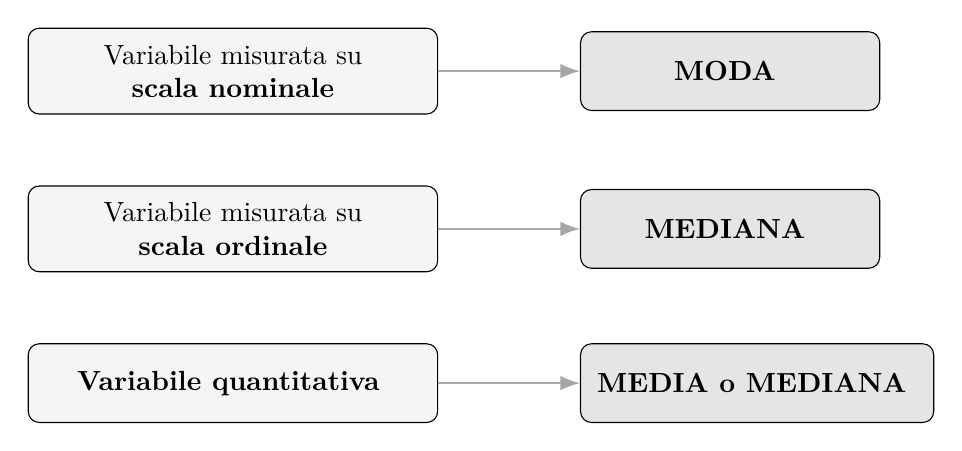
\begin{tikzpicture}[
  node distance=0.9cm and 1.8cm,
  boxleft/.style={
    draw,
    rounded corners=4pt,
    minimum width=5.2cm,
    minimum height=1.0cm,
    align=center,
    fill=gray!8,
    inner sep=6pt
  },
  boxright/.style={
    draw,
    rounded corners=4pt,
    minimum width=3.8cm,
    minimum height=1.0cm,
    align=center,
    fill=template!15,
    inner sep=6pt,
    font=\bfseries
  },
  arrow/.style={
    -{Latex[length=2.5mm]},
    thick,
    draw=gray!70
  }
]

\node[boxleft] (nom) {
Variabile misurata su\\
\textbf{scala nominale}
};

\node[boxleft, below=of nom] (ord) {
Variabile misurata su\\
\textbf{scala ordinale}
};

\node[boxleft, below=of ord] (quant) {
\textbf{Variabile quantitativa}
};

\node[boxright, right=of nom] (moda) {
MODA
};

\node[boxright, right=of ord] (mediana) {
MEDIANA
};

\node[boxright, right=of quant] (media) {
MEDIA o MEDIANA
};

\draw[arrow] (nom.east) -- (moda.west);
\draw[arrow] (ord.east) -- (mediana.west);
\draw[arrow] (quant.east) -- (media.west);

\end{tikzpicture}
\end{center}

\subsection{\texorpdfstring{Moda (\(Mo\))}{Moda (Mo)}}\label{moda-mo}

La moda \(Mo\) di una variabile \(X\) è la categoria a cui è associata
la massima frequenza:

\begin{center}
    $Mo(X) = \max(n_i)$ \\ (categoria con massimo valore di $n_i$)
\end{center}

\begin{tcolorbox}[enhanced jigsaw, toprule=.15mm, left=2mm, leftrule=.75mm, breakable, coltitle=black, title={Warning}, bottomtitle=1mm, opacitybacktitle=0.6, toptitle=1mm, titlerule=0mm, bottomrule=.15mm, colframe=quarto-callout-warning-color-frame, arc=.35mm, rightrule=.15mm, opacityback=0, colbacktitle=quarto-callout-warning-color!10!white, colback=white]

N.B: Si può calcolare per le variabili misurate a qualsiasi livello,
anche se di fatto viene calcolata solo per le variabile categoriali, in
quanto per altri livelli di misurazione si possono calcolare altri
indici più informativi

\end{tcolorbox}

\begin{Shaded}
\begin{Highlighting}[]
\NormalTok{opinione}
\end{Highlighting}
\end{Shaded}

\begin{verbatim}
                 categoria  n  N
1 Totalmente in disaccordo 10 10
2 Abbastanza in disaccordo  8 18
3             Indifferente  6 24
4     Abbastanza d'accordo 14 38
5     Totalmente d'accordo  3 41
\end{verbatim}

\begin{Shaded}
\begin{Highlighting}[]
\FunctionTok{max}\NormalTok{(opinione}\SpecialCharTok{$}\NormalTok{n) }\CommentTok{\# restituisce max(n\_i)}
\end{Highlighting}
\end{Shaded}

\begin{verbatim}
[1] 14
\end{verbatim}

\begin{Shaded}
\begin{Highlighting}[]
\CommentTok{\# va filtrato il dataframe per ottenere la categoria a cui }
\CommentTok{\# è associata la frequenza massima}
\NormalTok{opinione[opinione}\SpecialCharTok{$}\NormalTok{n }\SpecialCharTok{==} \FunctionTok{max}\NormalTok{(opinione}\SpecialCharTok{$}\NormalTok{n), }\StringTok{"categoria"}\NormalTok{]}
\end{Highlighting}
\end{Shaded}

\begin{verbatim}
[1] "Abbastanza d'accordo"
\end{verbatim}

\begin{Shaded}
\begin{Highlighting}[]
\CommentTok{\# codice alternativo che produce lo stesso risultato }
\NormalTok{opinione}\SpecialCharTok{$}\NormalTok{categoria[opinione}\SpecialCharTok{$}\NormalTok{n }\SpecialCharTok{==} \FunctionTok{max}\NormalTok{(opinione}\SpecialCharTok{$}\NormalTok{n)]}
\end{Highlighting}
\end{Shaded}

\begin{verbatim}
[1] "Abbastanza d'accordo"
\end{verbatim}

\subsection{Mediana}\label{mediana}

La mediana \(Me\) di una variabile \(X\) è la categoria che occupa la
posizione centrale o mediana (\(Pos_{Me}\)) nella distribuzione ordinata
dei dati, ovvero che è:

\begin{itemize}
\item preceduta da almeno 50\% dei casi
\item superata da almeno 50\% dei casi
\end{itemize}

\begin{equation*}
Pos_{Me} = \dfrac{(N+1)}{2}
\end{equation*}

Il valore di \(Pos_{Me}\) va cercato nella distribuzione delle frequenze
cumulate e si sceglie la categoria con \(N_i \geq Pos_{Me}\)

\subsection{Quantili}\label{quantili}

Categorie/valori che dividono la distribuzione di frequenza
\underline{ordinata} in più parti.

\begin{quote}
Qual è il reddito familiare che divide il 25\% dei più poveri dal restante 75\% ?
    
Qual è la soglia di reddito oltre cui sta la fascia dei più
    abbienti ?
    
Quali sono le persone che hanno performato al meglio nell'ultimo semestre?
\end{quote}

Il quantile \(x_p\) di ordine \(p\) della variabile \(X\) è quella
categoria/valore che è:

\begin{itemize}
\item preceduta da almeno $p$\% dei casi
\item superata da almeno $(1-p)$\% dei casi
\end{itemize}

\begin{center}
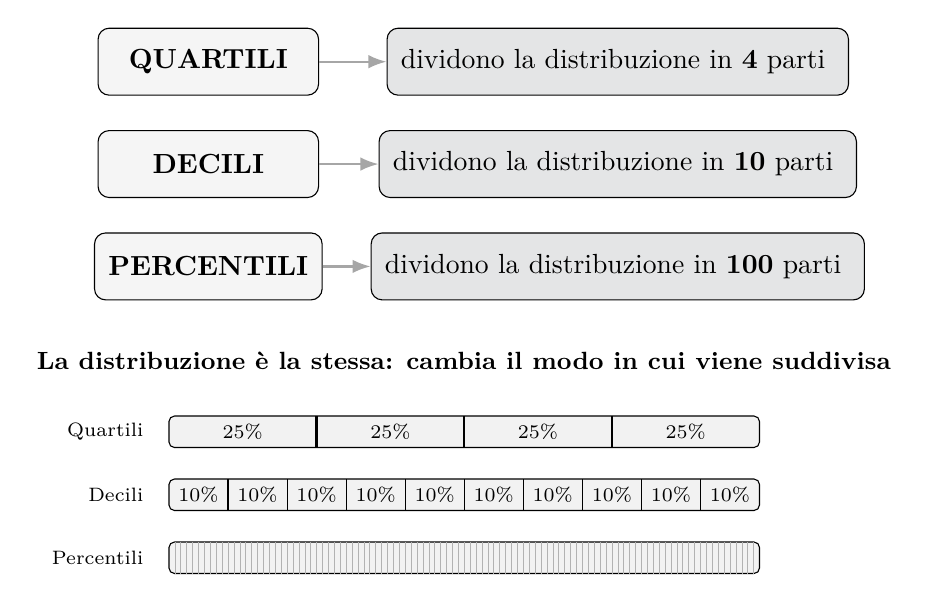
\begin{tikzpicture}[
  boxleft/.style={
    draw,
    rounded corners=4pt,
    minimum width=2.8cm,
    minimum height=0.85cm,
    align=center,
    fill=gray!8,
    inner sep=5pt,
    font=\bfseries
  },
  boxright/.style={
    draw,
    rounded corners=4pt,
    minimum width=5.0cm,
    minimum height=0.85cm,
    align=center,
    fill=template!15,
    inner sep=5pt
  },
  arrow/.style={
    -{Latex[length=2.3mm]},
    thick,
    draw=gray!70
  }
]

% Box superiori
\node[boxleft] (quartili) at (0,0) {QUARTILI};
\node[boxright] (qtext) at (5.2,0) {
dividono la distribuzione in \textbf{4} parti
};

\node[boxleft] (decili) at (0,-1.3) {DECILI};
\node[boxright] (dtext) at (5.2,-1.3) {
dividono la distribuzione in \textbf{10} parti
};

\node[boxleft] (percentili) at (0,-2.6) {PERCENTILI};
\node[boxright] (ptext) at (5.2,-2.6) {
dividono la distribuzione in \textbf{100} parti
};

% Frecce
\draw[arrow] (quartili.east) -- (qtext.west);
\draw[arrow] (decili.east) -- (dtext.west);
\draw[arrow] (percentili.east) -- (ptext.west);

% Testo sotto
\node[align=center, font=\small] at (3.3,-3.8) {
\textbf{La distribuzione è la stessa: cambia il modo in cui viene suddivisa}
};

% Barre: stessa lunghezza
\def\xstart{-0.5}
\def\xend{7.0}
\def\barheight{0.38}

% Quartili
\node[anchor=east, font=\scriptsize] at (-0.7,-4.7) {Quartili};
\draw[rounded corners=2pt, fill=gray!10]
  (\xstart,-4.9) rectangle (\xend,-4.5);

\foreach \x in {1.375,3.25,5.125}{
  \draw[thick] (\x,-4.9) -- (\x,-4.5);
}

\foreach \x in {0.4375,2.3125,4.1875,6.0625}{
  \node[font=\scriptsize] at (\x,-4.7) {25\%};
}

% Decili
\node[anchor=east, font=\scriptsize] at (-0.7,-5.5) {Decili};
\draw[rounded corners=2pt, fill=gray!10]
  (\xstart,-5.7) rectangle (\xend,-5.3);

\foreach \x in {0.25,1.0,1.75,2.5,3.25,4.0,4.75,5.5,6.25}{
  \draw[thin] (\x,-5.7) -- (\x,-5.3);
}

% Etichette 10% nei decili
\foreach \x in {-0.125,0.625,1.375,2.125,2.875,3.625,4.375,5.125,5.875,6.625}{
  \node[font=\scriptsize] at (\x,-5.5) {10\%};
}

% Percentili
\node[anchor=east, font=\scriptsize] at (-0.7,-6.3) {Percentili};
\draw[rounded corners=2pt, fill=gray!10]
  (\xstart,-6.5) rectangle (\xend,-6.1);

% tante suddivisioni sottili
\foreach \i in {1,...,99}{
  \pgfmathsetmacro{\x}{-0.5 + 7.5*\i/100}
  \draw[very thin, gray!60] (\x,-6.5) -- (\x,-6.1);
}

\end{tikzpicture}
\end{center}

Per il calcolo dei quantili di diverso ordine, il procedimento è analogo
a quello della Mediana, che di fatto è un caso particolare di questi
indici. In generale la Posizione di ordine \(p\) (in centesimi) si
ottiene:

\begin{equation*}
Pos_p = \dfrac{n+1}{100}\cdot p 
\end{equation*}

\subsubsection{\texorpdfstring{Trovare i quantili:
\texttt{quantile()}}{Trovare i quantili: quantile()}}\label{trovare-i-quantili-quantile}

\begin{verbatim}
quantile(x, probs = c(0, .25, .50, .75, 1))
\end{verbatim}

Funzione per il calcolo dei quantili da una variabile \(X\) (argomento
\texttt{x}) di diverso ordine (definito dall'argomento \texttt{probs}).
Di default, vengono calcolati i quartili, compresi anche il minimo
(\texttt{0}) e il massimo (\texttt{1}) della variabile \(X\).

\begin{Shaded}
\begin{Highlighting}[]
\FunctionTok{set.seed}\NormalTok{(}\DecValTok{123}\NormalTok{) }\CommentTok{\# garantisce la replicabilità dei risultati}
\NormalTok{x }\OtherTok{=} \FunctionTok{rnorm}\NormalTok{(}\DecValTok{1000}\NormalTok{, }\AttributeTok{mean =} \DecValTok{0}\NormalTok{, }\AttributeTok{sd =} \DecValTok{1}\NormalTok{)}
\FunctionTok{quantile}\NormalTok{(x)}
\end{Highlighting}
\end{Shaded}

\begin{verbatim}
          0%          25%          50%          75%         100% 
-2.809774679 -0.628324243  0.009209639  0.664601867  3.241039935 
\end{verbatim}

\begin{Shaded}
\begin{Highlighting}[]
\CommentTok{\# calcola i decili }
\FunctionTok{quantile}\NormalTok{(x, }\AttributeTok{probs =} \FunctionTok{seq}\NormalTok{(}\DecValTok{0}\NormalTok{,}\DecValTok{1}\NormalTok{, }\AttributeTok{by =}\NormalTok{ .}\DecValTok{10}\NormalTok{))}
\end{Highlighting}
\end{Shaded}

\begin{verbatim}
          0%          10%          20%          30%          40%          50% 
-2.809774679 -1.267328289 -0.788690220 -0.486452454 -0.214854912  0.009209639 
         60%          70%          80%          90%         100% 
 0.242040647  0.513088142  0.841412710  1.254751947  3.241039935 
\end{verbatim}

\subsection{Media}\label{media}

La media è una sorta di baricentro della distribuzione dei dati. Data
una variabile \(X\) composta da \(n\) valori:

\begin{equation*}
\bar{X} = \dfrac{\sum_{i = 1}^{n}x_i}{n}
\end{equation*}

\begin{center}
\scalebox{.80}{
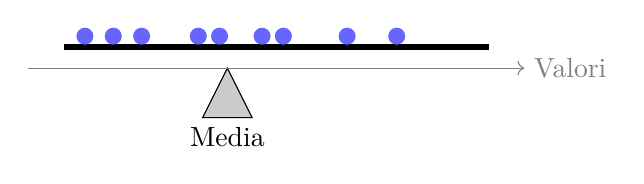
\begin{tikzpicture}[scale=0.9]

\def\data{0.8,1.2,1.6,2.4,2.7,3.3,3.6,4.5,5.2}
\def\mean{2.81}

% Tavola
\draw[line width=2pt] (0.5,0.3) -- (6.5,0.3);

% Fulcro
\draw[fill=gray!40]
(\mean,0) -- ++(-0.35,-0.7) -- ++(0.7,0) -- cycle;
\node[below] at (\mean,-0.7) {Media};

% Puntini = osservazioni
\foreach \x in \data {
    \fill[blue!60] (\x,0.45) circle (0.12);
}

% Asse
\draw[->, thin, gray] (0,0) -- (7,0) node[right] {Valori};

\end{tikzpicture}}
\end{center}

I dati: \(X = (0.8,1.2,1.6,2.4,2.7,3.3,3.6,4.5,5.2)\), la media
\(\bar{X} = 2.811\)

\begin{center}
\scalebox{.80}{
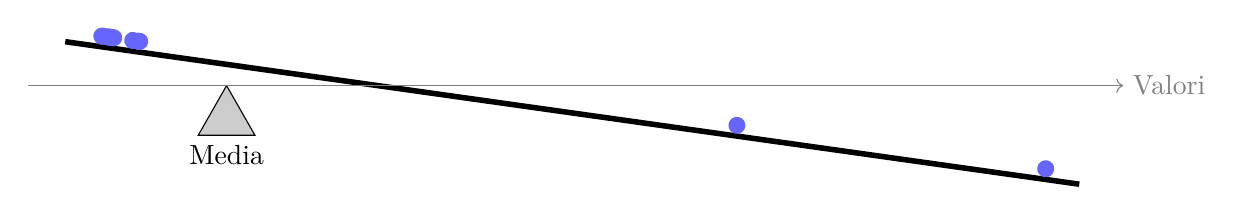
\begin{tikzpicture}[scale=0.9]

\def\data{1.18,1.02,1.10,1.16,1.01,1.10,1.05,1.12,1.45,1.52,1.54,1.55,10.06,14.46}
\def\mean{2.809}
\def\angle{8}

% ---- calcolo minimo e massimo ----
\pgfmathsetmacro{\xmin}{1.01}
\pgfmathsetmacro{\xmax}{14.46}

% piccolo margine estetico
\pgfmathsetmacro{\leftend}{\xmin - 0.5}
\pgfmathsetmacro{\rightend}{\xmax + 0.5}

% Fulcro
\draw[fill=gray!40]
(\mean,0) -- ++(-0.4,-0.7) -- ++(0.8,0) -- cycle;
\node[below] at (\mean,-0.7) {Media};

% Tavola + dati ruotati attorno al fulcro
\begin{scope}[rotate around={-\angle:(\mean,0.3)}]

    % Tavola che copre TUTTI i dati
    \draw[line width=2pt] (\leftend,0.3) -- (\rightend,0.3);

    % Puntini
    \foreach \x in \data {
        \fill[blue!60] (\x,0.45) circle (0.12);
    }

\end{scope}

% Asse
\draw[->, thin, gray] (\leftend-0.5,0) -- (\rightend+0.5,0) node[right] {Valori};

\end{tikzpicture}
}
\end{center}

I dati:
\(X = (1.18,1.02,1.10,1.16,1.01,1.10,1.05,1.12,1.45,1.52,1.54,1.55,10.06,14.46)\),
la media \(\bar{X} = 2.809\)

\subsubsection{\texorpdfstring{\texttt{mean()}}{mean()}}\label{mean}

\begin{verbatim}
mean(x, na.rm = FALSE)
\end{verbatim}

Funzione per calcolare la media di un vettore di valori \texttt{x}.
L'agromento \texttt{na.rm\ =\ TRUE} serve per ottenere il calcolo della
media nonostante la presenza di valori NA

\texttt{rowMeans()}: Calcola la media per ogni riga (quindi attraverso
le colonne)

\texttt{colMeans()}: Calcola la media per ogni colonna (quindi
attraverso le righe)

\begin{Shaded}
\begin{Highlighting}[]
\FunctionTok{mean}\NormalTok{(x)}
\end{Highlighting}
\end{Shaded}

\begin{verbatim}
[1] 0.01612787
\end{verbatim}

\section{Indici di variabilità}\label{indici-di-variabilituxe0}

Il concetto di variabilità si riferisce a quanto i punteggi di una
distribuzione sono sparsi, ovvero quanto siano simili o dissimili tra
loro.

\begin{itemize}
\tightlist
\item
  Il ricorso a un indice di tendenza centrale (come la media) comporta
  una forte semplificazione
\item
  È fondamentale capire quanto i dati siano dispersi intorno all'indice
  di tendenza centrale
\item
  La variabilità è una caratteristica fondamentale delle distribuzioni:
  \emph{``Variability is the essence of statistics''} (Cobb, 1992)
\end{itemize}

Gli indici di variabilità possono assumere solo valori positivi (non ha
senso parlare di dispersione negativa) o nulli (quando i dati hanno
tutti lo stesso valore).

\subsection{Campo di variazione (Gamma) o
range}\label{campo-di-variazione-gamma-o-range}

Il campo di variazione è la differenza tra il valore massimo e il valore
minimo osservato:

\[\text{gamma} = X_{max} - X_{min}\]

\begin{Shaded}
\begin{Highlighting}[]
\NormalTok{team\_A }\OtherTok{\textless{}{-}} \FunctionTok{c}\NormalTok{(}\DecValTok{38}\NormalTok{, }\DecValTok{42}\NormalTok{, }\DecValTok{44}\NormalTok{, }\DecValTok{36}\NormalTok{, }\DecValTok{39}\NormalTok{, }\DecValTok{42}\NormalTok{, }\DecValTok{38}\NormalTok{, }\DecValTok{41}\NormalTok{)}
\FunctionTok{max}\NormalTok{(team\_A) }\SpecialCharTok{{-}} \FunctionTok{min}\NormalTok{(team\_A)}
\end{Highlighting}
\end{Shaded}

\begin{verbatim}
[1] 8
\end{verbatim}

\begin{tcolorbox}[enhanced jigsaw, toprule=.15mm, left=2mm, leftrule=.75mm, breakable, coltitle=black, title={Limitazione}, bottomtitle=1mm, opacitybacktitle=0.6, toptitle=1mm, titlerule=0mm, bottomrule=.15mm, colframe=quarto-callout-caution-color-frame, arc=.35mm, rightrule=.15mm, opacityback=0, colbacktitle=quarto-callout-caution-color!10!white, colback=white]

Dipende solo da due valori (massimo e minimo) e non considera la
distribuzione dei dati intermedi.

\end{tcolorbox}

\subsection{La varianza}\label{la-varianza}

La varianza \(\sigma^2\) è la media degli scarti al quadrato tra i dati
e la media:

\[\sigma^2 = \frac{\sum_i^n (X_i - \bar{X})^2}{n}\]

La varianza assume valore minimo \(0\) quando tutti i dati sono uguali
tra loro e aumenta all'aumentare della dispersione.

\begin{tcolorbox}[enhanced jigsaw, toprule=.15mm, left=2mm, leftrule=.75mm, breakable, coltitle=black, title={Important}, bottomtitle=1mm, opacitybacktitle=0.6, toptitle=1mm, titlerule=0mm, bottomrule=.15mm, colframe=quarto-callout-important-color-frame, arc=.35mm, rightrule=.15mm, opacityback=0, colbacktitle=quarto-callout-important-color!10!white, colback=white]

La funzione \texttt{var()} di R calcola la \textbf{varianza
campionaria}, che divide per \(n-1\) anziché \(n\). Per dati descrittivi
(popolazione osservata) si usa \(n\); per stimare la varianza della
popolazione da un campione si usa \(n-1\).

\end{tcolorbox}

\subsection{La deviazione standard}\label{la-deviazione-standard}

La deviazione standard è la radice della varianza:

\[\sigma = \sqrt{\sigma^2}\]

Riporta l'indice di variabilità sulla \textbf{scala della variabile}.

Esempio: Se in un campione di dipendenti la variabile
\texttt{WorkHoursPerWeek} ha media \(40\) ore e deviazione standard
\(2.5\), i dipendenti differiscono mediamente di \(2.5\) ore dal carico
di lavoro medio.

La deviazione standard, a differenza della varianza, è espressa nella
stessa unità di misura della variabile.

\subsection{Il coefficiente di
variazione}\label{il-coefficiente-di-variazione}

Il coefficiente di variazione è il rapporto tra la deviazione standard e
il valore assoluto della media:

\[CV = \frac{\sigma}{|\bar{X}|}\]

Il CV è un indice di \textbf{variabilità relativa} fondamentale per
eseguire \textbf{confronti} tra fenomeni misurati su \textbf{scale
diverse}.

\subsection{Differenza interquartilica
(IQR)}\label{differenza-interquartilica-iqr}

La differenza interquartilica è la differenza tra il terzo e il primo
quartile:

\[IQR = Q_{75} - Q_{25}\]

L'IQR misura la dispersione del 50\% centrale dei dati ed è un indice
\textbf{robusto} perché i valori estremi incidono poco o per nulla.

\textbf{Outlier:} valori oltre
\([Q_1 - 1.5 \times IQR \;;\; Q_3 + 1.5 \times IQR]\).

Il \textbf{boxplot} (vedi sezione Section~\ref{sec-boxplot}) visualizza
Q1, mediana, Q3 e gli outlier in un unico grafico.

La funzione \texttt{IQR(x)} permette di calcolare la differenza
interquartilica in R per qualsiasi variabile quantitativa.

\section{Perché i grafici}\label{perchuxe9-i-grafici}

\begin{quote}
\large
Graphs remind us that the process of statistical inference is
not mechanical. This process often involves subjective decisions (e.g., the
evaluation, exploration, and/or deletion of outliers) which are an
integral part of the analysis. Thus, graphs are among the most
appropriate tools to enhance transparency and confer plausibility
to such decisions.
\end{quote}

\vspace{10mm}
\begin{flushright}
Pastore et al. (2017)
\end{flushright}

Data set di Anscombe (Table~\ref{tbl-AnsCombe}): Quattro dataset, di
seguito le statistiche descrittive realitive alla variabile x e alla
variabile y e la loro correlazione:

\begin{table}

\caption{\label{tbl-AnsCombe}Dataset di Anscombe}

\centering{

\begin{tabular}{lccccc}
\toprule
Dataset & Media.X & Media.Y & Varianza.X & Varianza.Y & Correlazione\\
\midrule
Dataset 1 & 9 & 7.5 & 11 & 4.13 & 0.82\\
Dataset 2 & 9 & 7.5 & 11 & 4.13 & 0.82\\
Dataset 3 & 9 & 7.5 & 11 & 4.12 & 0.82\\
Dataset 4 & 9 & 7.5 & 11 & 4.12 & 0.82\\
\bottomrule
\end{tabular}

}

\end{table}%

Guardando la \textbf{?@tbl-Anscombe}, sembra che i quattro dataset siano
identici, in termini di media, varianza e correlazione tra le variabili
\(x\) e \(y\). Tuttavia, se si guardano i grafici a dispersione (vedi
\textbf{?@sec-correlazione}) tra le variabili \(x\) e \(y\) dei quattro
dataset (Figure~\ref{fig-data}), appaiono delle differenze abbastanza
palesi tra i diversi dataset.

\begin{figure}

\begin{minipage}{0.50\linewidth}

\centering{

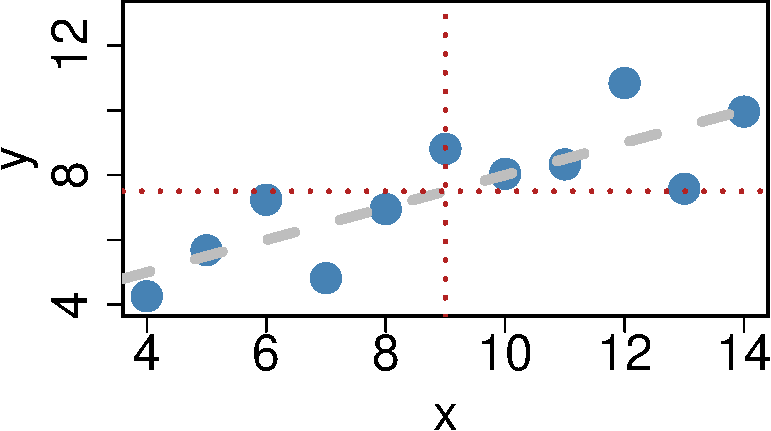
\includegraphics[width=0.7\linewidth,height=\textheight,keepaspectratio]{dispensa-statistica-descrittiva_files/figure-pdf/fig-data-1.pdf}

}

\subcaption{\label{fig-data-1}Dataset 1}

\end{minipage}%
%
\begin{minipage}{0.50\linewidth}

\centering{

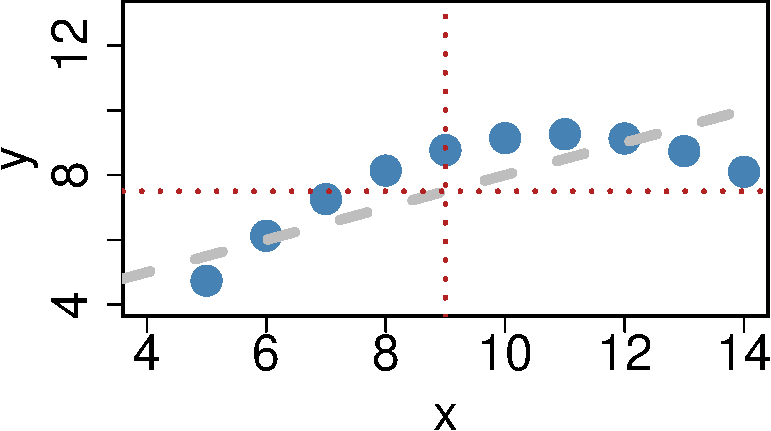
\includegraphics[width=0.7\linewidth,height=\textheight,keepaspectratio]{dispensa-statistica-descrittiva_files/figure-pdf/fig-data-2.pdf}

}

\subcaption{\label{fig-data-2}Dataset 2}

\end{minipage}%
\newline
\begin{minipage}{0.50\linewidth}

\centering{

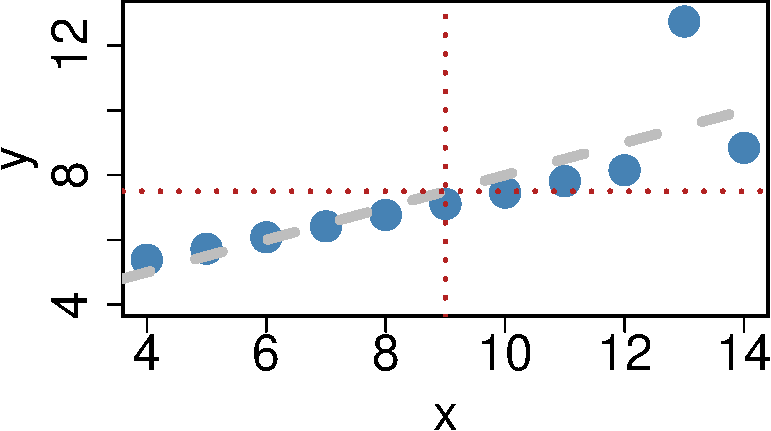
\includegraphics[width=0.7\linewidth,height=\textheight,keepaspectratio]{dispensa-statistica-descrittiva_files/figure-pdf/fig-data-3.pdf}

}

\subcaption{\label{fig-data-3}Dataset 3}

\end{minipage}%
%
\begin{minipage}{0.50\linewidth}

\centering{

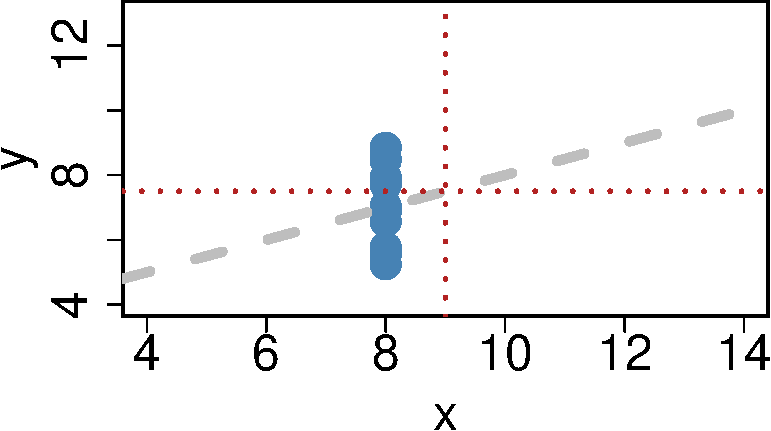
\includegraphics[width=0.7\linewidth,height=\textheight,keepaspectratio]{dispensa-statistica-descrittiva_files/figure-pdf/fig-data-4.pdf}

}

\subcaption{\label{fig-data-4}Dataset 4}

\end{minipage}%

\caption{\label{fig-data}I grafici raccontano un'altra storia}

\end{figure}%

\section{Grafici}\label{grafici}

R fornisce uno strumento molto utile per la rappresentazione grafica dei
dati e dei risultati già con il suo pacchetto base \texttt{graphics}

\begin{tcolorbox}[enhanced jigsaw, toprule=.15mm, left=2mm, leftrule=.75mm, breakable, coltitle=black, title={NB}, bottomtitle=1mm, opacitybacktitle=0.6, toptitle=1mm, titlerule=0mm, bottomrule=.15mm, colframe=quarto-callout-warning-color-frame, arc=.35mm, rightrule=.15mm, opacityback=0, colbacktitle=quarto-callout-warning-color!10!white, colback=white]

Non avete bisogno di installarlo, è caricato automaticamente nel momento
in cui scaricate R e le sue funzioni sono sempre disponibili

\end{tcolorbox}

\texttt{ggplot2} è un pacchetto più avanzato per la creazione dei
grafici. Non entreremo nel dettaglio del suo funzionamento perché è un
po' più complicato

Alcune funzioni incluse nel pacchetto \texttt{graphics}:

\phantomsection\label{annotated-cell-96}%
\begin{Shaded}
\begin{Highlighting}[]
\FunctionTok{plot}\NormalTok{(x) }\hspace*{\fill}\NormalTok{\circled{1}}
\FunctionTok{plot}\NormalTok{(x, y) }\hspace*{\fill}\NormalTok{\circled{2}}
\FunctionTok{hist}\NormalTok{(x) }\hspace*{\fill}\NormalTok{\circled{3}}
\FunctionTok{boxplot}\NormalTok{(x) }\hspace*{\fill}\NormalTok{\circled{4}}
\FunctionTok{barplot}\NormalTok{(x) }\hspace*{\fill}\NormalTok{\circled{5}}
\end{Highlighting}
\end{Shaded}

\begin{description}
\tightlist
\item[\circled{1}]
Grafico di una variabile quantitativa
\item[\circled{2}]
Grafico a dispersione di due variabili quantitative (vedi
\textbf{?@sec-correlazione})
\item[\circled{3}]
Istogramma di una variabile quantitativa (Section~\ref{sec-hist})
\item[\circled{4}]
Boxplot della distribuzione quartile di una (o più) variabili
(Section~\ref{sec-boxplot})
\item[\circled{5}]
Grafico a barre per le frequenze delle variabili qualitative
(Section~\ref{sec-barplot})
\end{description}

\subsection{Grafico a barre}\label{sec-barplot}

Usato per variabili qualitative nominali o ordinali:

\begin{itemize}
\tightlist
\item
  Asse \(x\): categoria \(k\)
\item
  Asse \(y\): Frequenza \(n_k\) (vale anche per le frequenze
  percentuali)
\end{itemize}

L'altezza della barretta è proporzionale alla sua frequenza

\begin{verbatim}
barplot(x)
\end{verbatim}

Dove \texttt{x} è il vettore delle frequenze (quello che si ottiene
applicando la funzione \texttt{table()} a una variabile categoriale)

\begin{center}
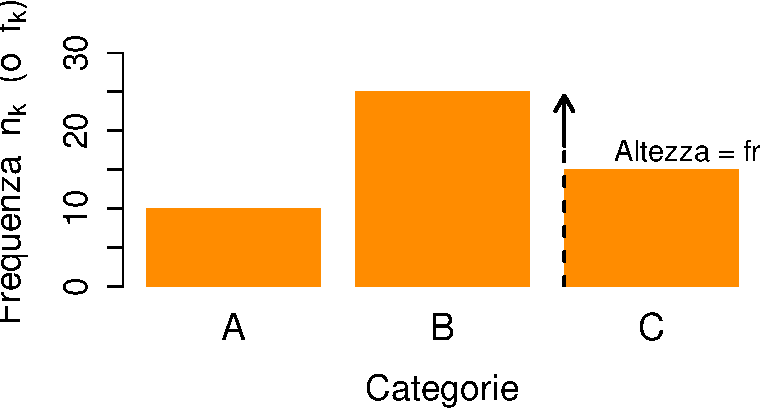
\includegraphics[width=0.7\linewidth,height=\textheight,keepaspectratio]{dispensa-statistica-descrittiva_files/figure-pdf/unnamed-chunk-79-1.pdf}
\end{center}

\begin{table}

\caption{\label{tbl-examples}Tabelle di frequenza per le categorie A, B,
C.}

\begin{minipage}{0.50\linewidth}

\begin{longtable}[]{@{}cc@{}}
\toprule\noalign{}
Categoria & \(n_k\) \\
\midrule\noalign{}
\endhead
\bottomrule\noalign{}
\endlastfoot
A & 21 \\
B & 24 \\
C & 22 \\
\end{longtable}

\end{minipage}%
%
\begin{minipage}{0.50\linewidth}

\begin{longtable}[]{@{}cc@{}}
\toprule\noalign{}
Categoria & \(n_k\) \\
\midrule\noalign{}
\endhead
\bottomrule\noalign{}
\endlastfoot
A & 12 \\
B & 35 \\
C & 18 \\
\end{longtable}

\end{minipage}%

\end{table}%

\begin{figure}

\begin{minipage}{0.50\linewidth}

\begin{figure}[H]

\centering{

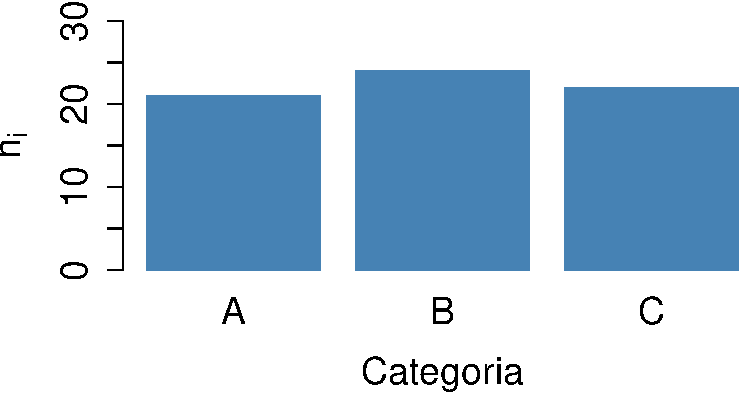
\includegraphics[width=0.7\linewidth,height=\textheight,keepaspectratio]{dispensa-statistica-descrittiva_files/figure-pdf/fig-examples-1.pdf}

}

\caption{\label{fig-examples-1}Barplot delle tabelle}

\end{figure}%

\end{minipage}%
%
\begin{minipage}{0.50\linewidth}

\begin{figure}[H]

\centering{

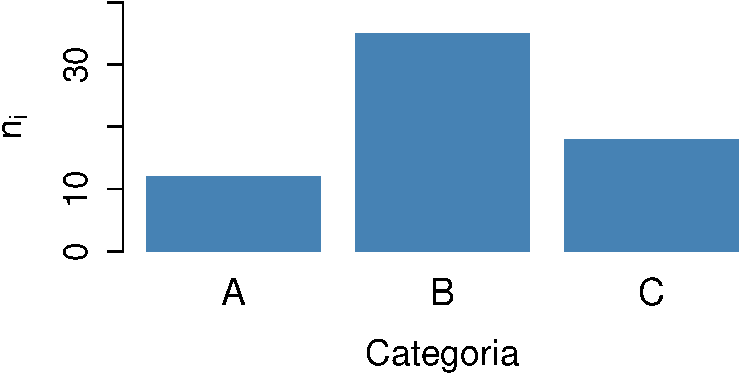
\includegraphics[width=0.7\linewidth,height=\textheight,keepaspectratio]{dispensa-statistica-descrittiva_files/figure-pdf/fig-examples-2.pdf}

}

\caption{\label{fig-examples-2}Barplot delle tabelle}

\end{figure}%

\end{minipage}%

\end{figure}%

\begin{Shaded}
\begin{Highlighting}[]
\NormalTok{dati }\OtherTok{=} \FunctionTok{factor}\NormalTok{(}\FunctionTok{rep}\NormalTok{(}\FunctionTok{c}\NormalTok{(}\StringTok{"A"}\NormalTok{, }\StringTok{"B"}\NormalTok{, }\StringTok{"C"}\NormalTok{), }\FunctionTok{c}\NormalTok{(}\DecValTok{12}\NormalTok{, }\DecValTok{35}\NormalTok{, }\DecValTok{18}\NormalTok{))); dati}
\end{Highlighting}
\end{Shaded}

\begin{verbatim}
 [1] A A A A A A A A A A A A B B B B B B B B B B B B B B B B B B B B B B B B B B
[39] B B B B B B B B B C C C C C C C C C C C C C C C C C C
Levels: A B C
\end{verbatim}

\begin{Shaded}
\begin{Highlighting}[]
\FunctionTok{table}\NormalTok{(dati)}
\end{Highlighting}
\end{Shaded}

\begin{verbatim}
dati
 A  B  C 
12 35 18 
\end{verbatim}

\begin{Shaded}
\begin{Highlighting}[]
\FunctionTok{barplot}\NormalTok{(}\FunctionTok{table}\NormalTok{(dati), }\AttributeTok{col =} \StringTok{"darkgreen"}\NormalTok{)}
\end{Highlighting}
\end{Shaded}

\begin{center}
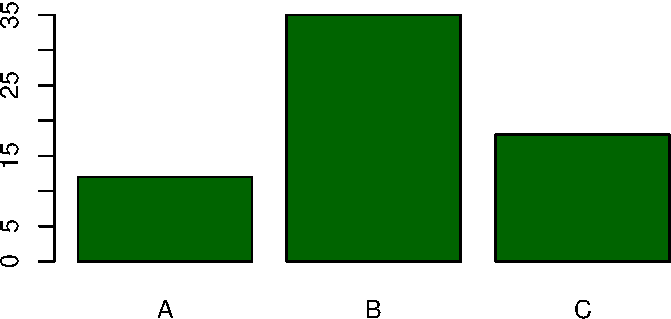
\includegraphics[width=0.3\linewidth,height=\textheight,keepaspectratio]{dispensa-statistica-descrittiva_files/figure-pdf/unnamed-chunk-80-1.pdf}
\end{center}

\subsection{Istogrammi}\label{sec-hist}

\texttt{hist(x,\ breaks)} produce un istogramma a partire da un vettore
\texttt{x} di osservazioni quantitative.

Per costruire l'istogramma, l'intervallo dei valori di \texttt{x} viene
diviso in classi contigue, disposte sull'asse delle \(x\). Per ogni
classe si conta quante osservazioni vi ricadono: questa frequenza è
l'altezza della barra sull'asse delle \(y\).

L'argomento \texttt{breaks} stabilisce come vengono costruite le classi.
Può essere il numero di classi desiderato, una regola per calcolarlo
(\texttt{"Sturges"}, il default, \texttt{"FD"} o \texttt{"Scott"}),
oppure un vettore con i punti di taglio esatti. Il numero di classi
determina la loro ampiezza:

\begin{itemize}
\tightlist
\item
  \textbf{Classi strette (molti \texttt{breaks})}: ogni classe raccoglie
  poche osservazioni, quindi le barre sono basse e alcune classi possono
  restare vuote. L'istogramma risulta frastagliato e difficile da
  leggere.
\item
  \textbf{Classi larghe (pochi \texttt{breaks})}: ogni classe raccoglie
  molte osservazioni, quindi le barre sono più alte ma sono poche.
  L'istogramma diventa troppo grossolano e nasconde la forma della
  distribuzione.
\end{itemize}

\begin{tcolorbox}[enhanced jigsaw, toprule=.15mm, left=2mm, leftrule=.75mm, breakable, coltitle=black, title={Note}, bottomtitle=1mm, opacitybacktitle=0.6, toptitle=1mm, titlerule=0mm, bottomrule=.15mm, colframe=quarto-callout-note-color-frame, arc=.35mm, rightrule=.15mm, opacityback=0, colbacktitle=quarto-callout-note-color!10!white, colback=white]

Quando \texttt{breaks} è un numero, R lo usa come \emph{suggerimento} e
lo arrotonda a intervalli ``puliti''. Per questo con
\texttt{breaks\ =\ 145} non si ottengono esattamente 145 barre.

\end{tcolorbox}

\begin{figure}

\begin{minipage}{0.50\linewidth}

\begin{figure}[H]

{\centering 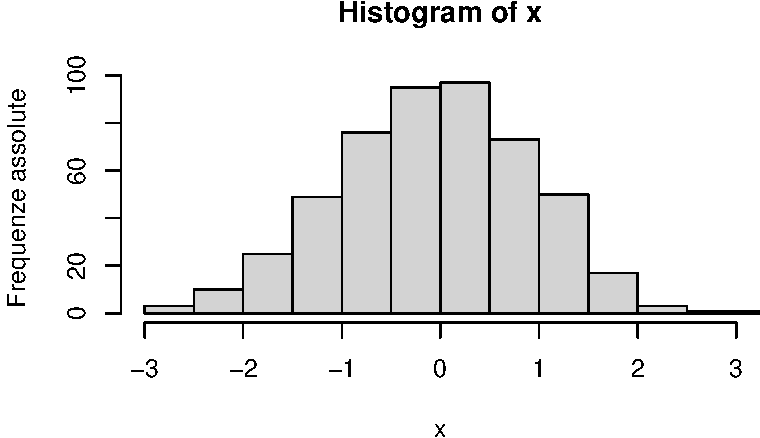
\includegraphics[width=0.7\linewidth,height=\textheight,keepaspectratio]{dispensa-statistica-descrittiva_files/figure-pdf/unnamed-chunk-81-1.pdf}

}

\subcaption{n = 500}

\end{figure}%

\end{minipage}%
%
\begin{minipage}{0.50\linewidth}

\begin{figure}[H]

{\centering 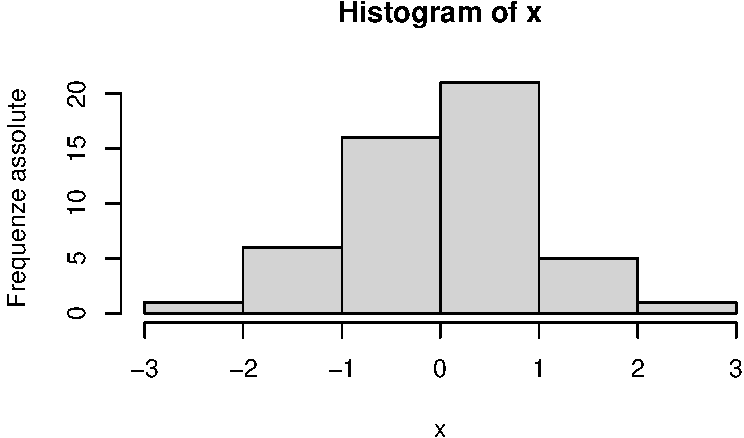
\includegraphics[width=0.7\linewidth,height=\textheight,keepaspectratio]{dispensa-statistica-descrittiva_files/figure-pdf/unnamed-chunk-81-2.pdf}

}

\subcaption{n = 50}

\end{figure}%

\end{minipage}%
\newline
\begin{minipage}{0.50\linewidth}
Istogrammi con n diverso\end{minipage}%

\end{figure}%

\begin{Shaded}
\begin{Highlighting}[]
\NormalTok{x }\OtherTok{=} \FunctionTok{rnorm}\NormalTok{(}\DecValTok{500}\NormalTok{, }\AttributeTok{mean =} \DecValTok{0}\NormalTok{, }\AttributeTok{sd =} \DecValTok{1}\NormalTok{)}
\FunctionTok{hist}\NormalTok{(x)}
\end{Highlighting}
\end{Shaded}

\begin{center}
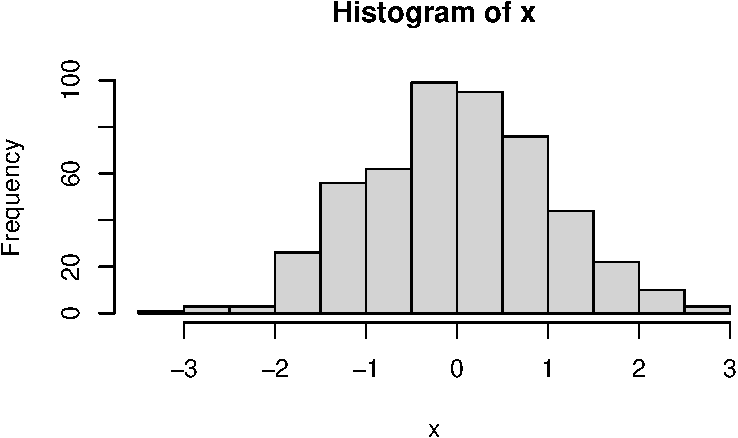
\includegraphics[width=0.7\linewidth,height=\textheight,keepaspectratio]{dispensa-statistica-descrittiva_files/figure-pdf/unnamed-chunk-82-1.pdf}
\end{center}

\begin{center}
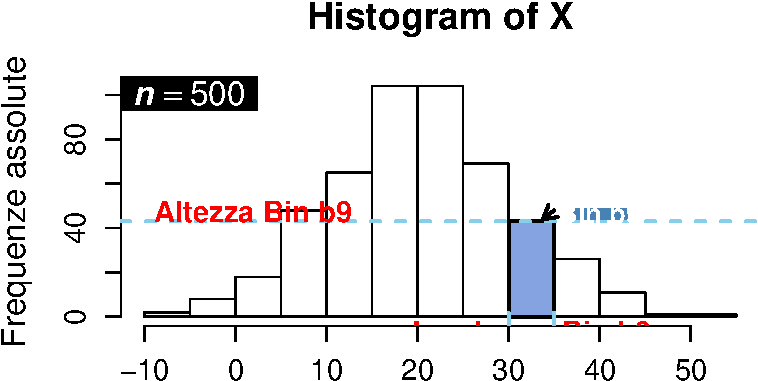
\includegraphics[width=0.7\linewidth,height=\textheight,keepaspectratio]{dispensa-statistica-descrittiva_files/figure-pdf/unnamed-chunk-83-1.pdf}
\end{center}

\begin{figure}

\begin{minipage}{0.50\linewidth}

\centering{

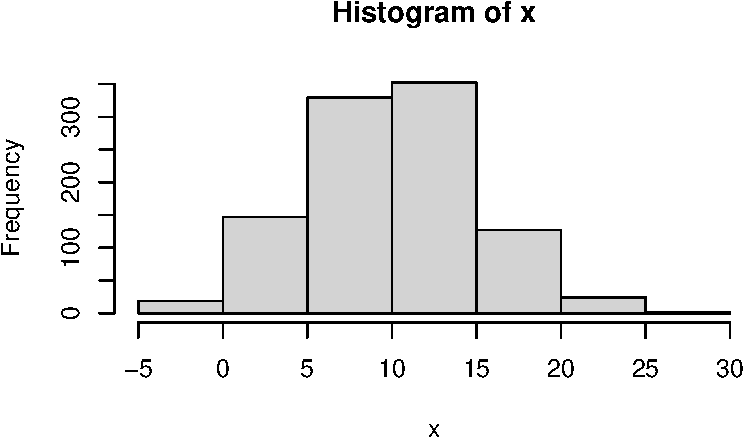
\includegraphics[width=0.8\linewidth,height=\textheight,keepaspectratio]{dispensa-statistica-descrittiva_files/figure-pdf/fig-methods-1.pdf}

}

\subcaption{\label{fig-methods-1}Sturges - Default}

\end{minipage}%
%
\begin{minipage}{0.50\linewidth}

\centering{

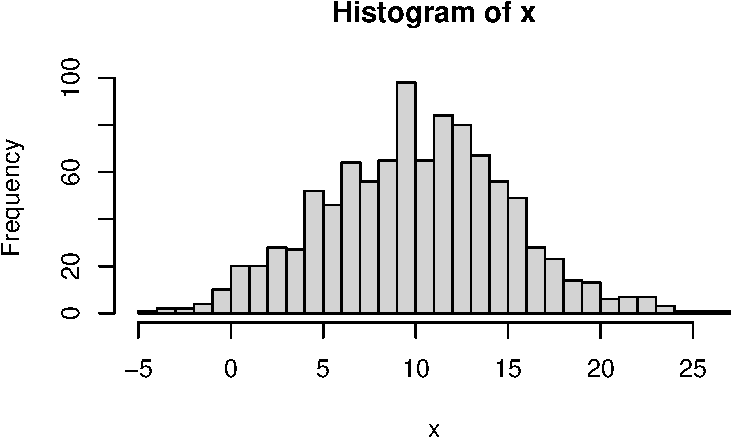
\includegraphics[width=0.8\linewidth,height=\textheight,keepaspectratio]{dispensa-statistica-descrittiva_files/figure-pdf/fig-methods-2.pdf}

}

\subcaption{\label{fig-methods-2}FD}

\end{minipage}%
\newline
\begin{minipage}{0.50\linewidth}

\centering{

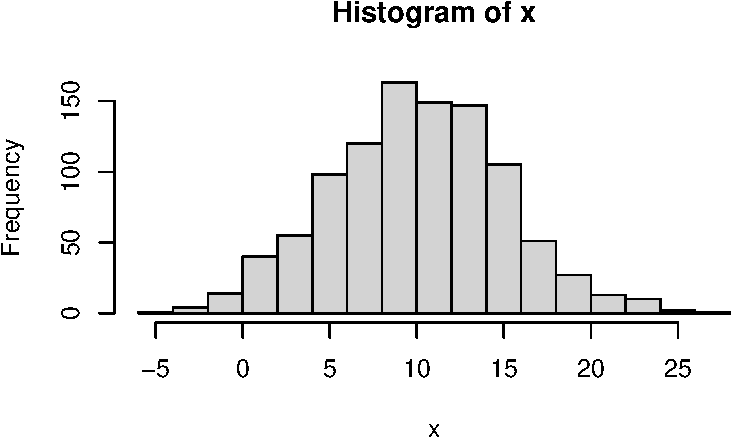
\includegraphics[width=0.8\linewidth,height=\textheight,keepaspectratio]{dispensa-statistica-descrittiva_files/figure-pdf/fig-methods-3.pdf}

}

\subcaption{\label{fig-methods-3}Scott}

\end{minipage}%
%
\begin{minipage}{0.50\linewidth}

\centering{

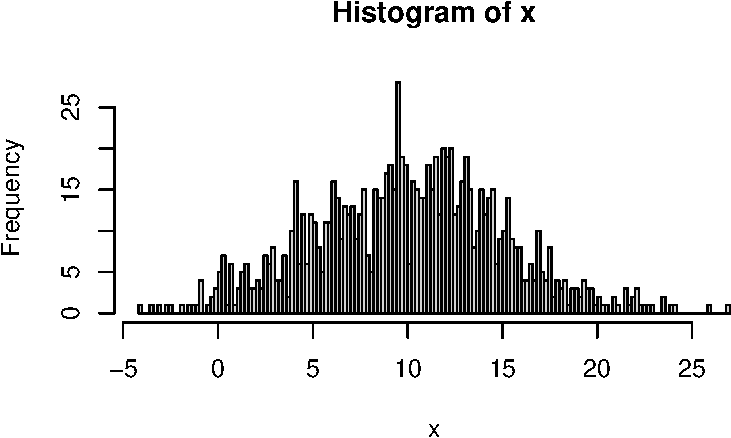
\includegraphics[width=0.8\linewidth,height=\textheight,keepaspectratio]{dispensa-statistica-descrittiva_files/figure-pdf/fig-methods-4.pdf}

}

\subcaption{\label{fig-methods-4}User defined (145)}

\end{minipage}%

\caption{\label{fig-methods}Metodi per la definizione dei breaks}

\end{figure}%

\begin{center}
Sturges: 

$\displaystyle \frac{\max(x) - \min(x)}{\log_{2}(n + 1)}$

Scott: 

 $\displaystyle 3.5 \sqrt{\mathrm{var}(x)} \, n^{-1/3}$
 
Freedman-Diaconis 
 
 $\displaystyle 2 \,(Q_3 - Q_1)\, n^{-1/3}$ 
 
User defined: 

 $\displaystyle \dfrac{\max(x) - \min(x)}{\text{breaks}}$ 

\end{center}

\subsection{Boxplot}\label{sec-boxplot}

\texttt{boxplot(x)} Produce un boxplot a partire da un vettore X di
osservazioni quantitative.

\begin{center}
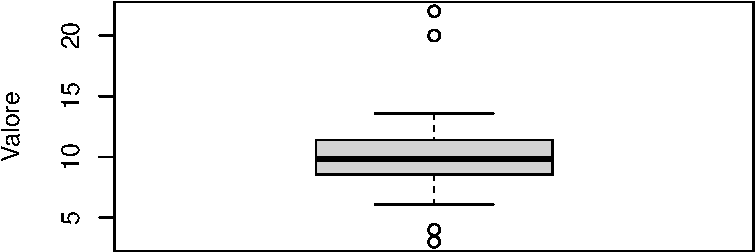
\includegraphics[width=0.7\linewidth,height=\textheight,keepaspectratio]{dispensa-statistica-descrittiva_files/figure-pdf/unnamed-chunk-85-1.pdf}
\end{center}

\begin{center}
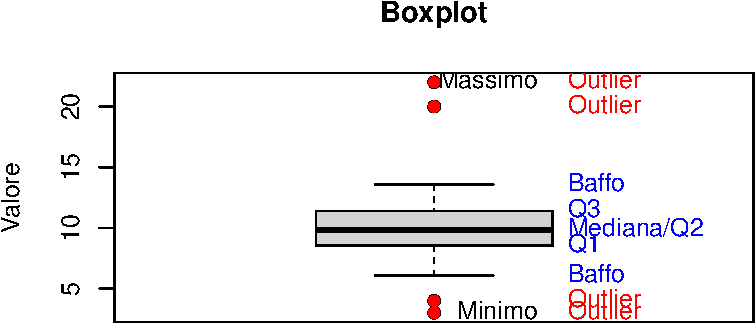
\includegraphics[width=0.7\linewidth,height=\textheight,keepaspectratio]{dispensa-statistica-descrittiva_files/figure-pdf/unnamed-chunk-86-1.pdf}
\end{center}

\subsection{Boxplot -- Calcolo degli
outlier}\label{boxplot-calcolo-degli-outlier}

La lunghezza dei baffi (e di conseguenza la definizione degli outliers)
è definita attraverso il metodo Tukey:

\[[Q_1 - 1.5 \times IQR, \, Q_3 + 1.5 \times IQR]\]

dove \(IQR = Q_3 - Q_1\) (Inter-quartile range)

Tutti i valori che cadono al di fuori dei baffi, sono definiti outliers.

Settando l'argomento \texttt{range\ =\ x} si può cambiare il modo in cui
vengono calcolati i baffi:

\begin{Shaded}
\begin{Highlighting}[]
\FunctionTok{boxplot}\NormalTok{(x, }\AttributeTok{range =} \DecValTok{2}\NormalTok{)}
\FunctionTok{boxplot}\NormalTok{(x, }\AttributeTok{range =} \DecValTok{0}\NormalTok{)}
\end{Highlighting}
\end{Shaded}

\begin{figure}

\begin{minipage}{0.50\linewidth}

\begin{figure}[H]

{\centering 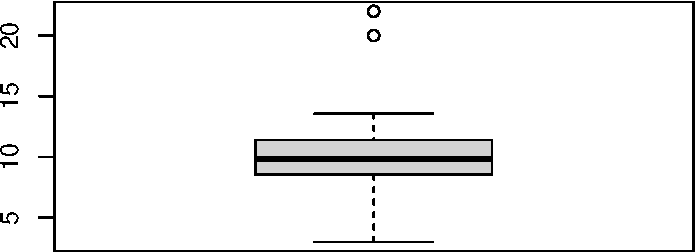
\includegraphics[width=0.7\linewidth,height=\textheight,keepaspectratio]{dispensa-statistica-descrittiva_files/figure-pdf/unnamed-chunk-87-1.pdf}

}

\subcaption{range = 2 - Meno Conservativo}

\end{figure}%

\end{minipage}%
%
\begin{minipage}{0.50\linewidth}

\begin{figure}[H]

{\centering 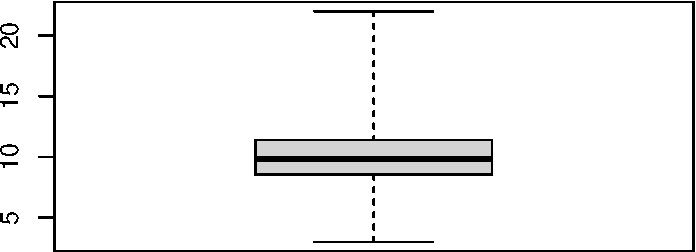
\includegraphics[width=0.7\linewidth,height=\textheight,keepaspectratio]{dispensa-statistica-descrittiva_files/figure-pdf/unnamed-chunk-87-2.pdf}

}

\subcaption{range = 0 - Minimo e Massimo}

\end{figure}%

\end{minipage}%
\newline
\begin{minipage}{0.50\linewidth}
Calcolo degli outlier\end{minipage}%

\end{figure}%

\section{Esempi}\label{esempi}

\subsection{\texorpdfstring{\texttt{barplot()}}{barplot()}}\label{barplot}

\begin{Shaded}
\begin{Highlighting}[]
\NormalTok{voto }\OtherTok{=} \FunctionTok{sample}\NormalTok{(}\FunctionTok{rep}\NormalTok{(}\FunctionTok{c}\NormalTok{(}\StringTok{"si"}\NormalTok{, }\StringTok{"no"}\NormalTok{, }\StringTok{"astenuti"}\NormalTok{), }
           \FunctionTok{c}\NormalTok{(}\DecValTok{12}\NormalTok{, }\DecValTok{15}\NormalTok{, }\DecValTok{2}\NormalTok{)))}
\NormalTok{voto }\OtherTok{=} \FunctionTok{factor}\NormalTok{(voto, }\AttributeTok{levels =} \FunctionTok{c}\NormalTok{(}\StringTok{"si"}\NormalTok{, }\StringTok{"no"}\NormalTok{, }\StringTok{"astenuti"}\NormalTok{))}
\FunctionTok{table}\NormalTok{(voto)}

\CommentTok{\# le frequenze restituite dalla funzione table() vanno usate }
\CommentTok{\# come vettore di base per il barplot}

\FunctionTok{barplot}\NormalTok{(}\FunctionTok{table}\NormalTok{(voto), }
        \AttributeTok{col =} \FunctionTok{c}\NormalTok{(}\StringTok{"darkgreen"}\NormalTok{, }\StringTok{"darkred"}\NormalTok{, }\StringTok{"darkblue"}\NormalTok{), }
        \AttributeTok{ylim =} \FunctionTok{c}\NormalTok{(}\DecValTok{0}\NormalTok{, }\DecValTok{20}\NormalTok{))}
\end{Highlighting}
\end{Shaded}

\begin{verbatim}
voto
      si       no astenuti 
      12       15        2 
\end{verbatim}

\begin{Shaded}
\begin{Highlighting}[]
\FunctionTok{barplot}\NormalTok{(}\FunctionTok{table}\NormalTok{(voto), }
        \AttributeTok{col =} \FunctionTok{c}\NormalTok{(}\StringTok{"darkgreen"}\NormalTok{, }\StringTok{"darkred"}\NormalTok{, }\StringTok{"darkblue"}\NormalTok{), }
        \AttributeTok{ylim =} \FunctionTok{c}\NormalTok{(}\DecValTok{0}\NormalTok{, }\DecValTok{20}\NormalTok{))}
\end{Highlighting}
\end{Shaded}

\begin{center}
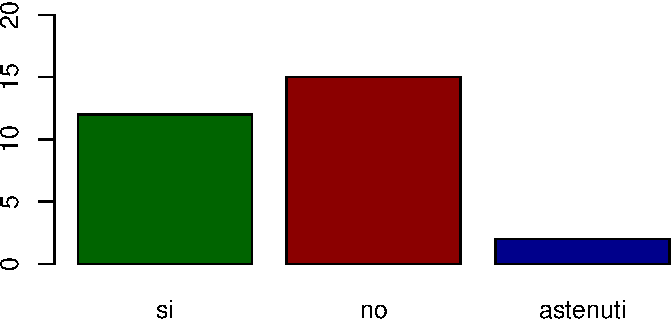
\includegraphics[width=0.7\linewidth,height=\textheight,keepaspectratio]{dispensa-statistica-descrittiva_files/figure-pdf/unnamed-chunk-90-1.pdf}
\end{center}

\subsection{\texorpdfstring{\texttt{boxplot()}}{boxplot()}}\label{boxplot}

\begin{figure}

\begin{minipage}{0.33\linewidth}

\centering{

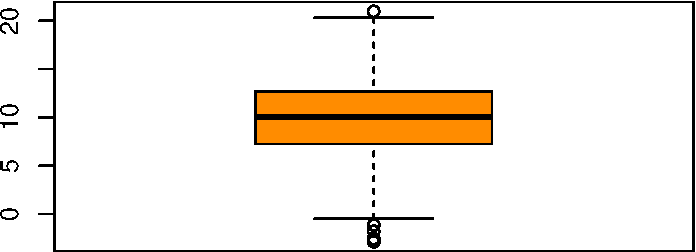
\includegraphics[width=1\linewidth,height=\textheight,keepaspectratio]{dispensa-statistica-descrittiva_files/figure-pdf/fig-boxes-1.pdf}

}

\subcaption{\label{fig-boxes-1}boxplot(x)}

\end{minipage}%
%
\begin{minipage}{0.33\linewidth}

\centering{

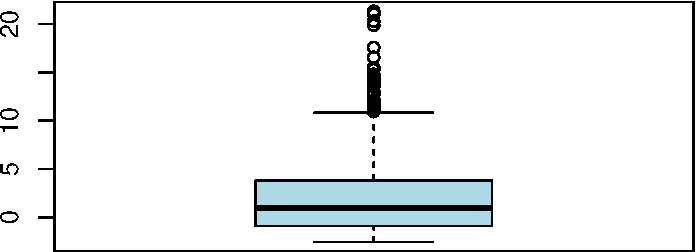
\includegraphics[width=1\linewidth,height=\textheight,keepaspectratio]{dispensa-statistica-descrittiva_files/figure-pdf/fig-boxes-2.pdf}

}

\subcaption{\label{fig-boxes-2}boxplot(y)}

\end{minipage}%
%
\begin{minipage}{0.33\linewidth}

\centering{

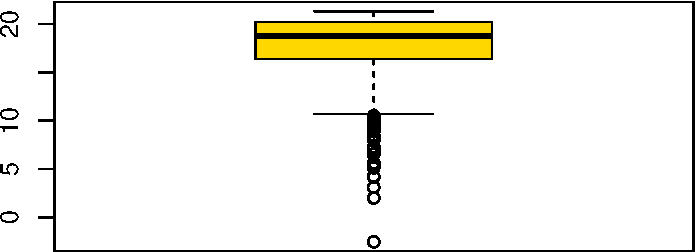
\includegraphics[width=1\linewidth,height=\textheight,keepaspectratio]{dispensa-statistica-descrittiva_files/figure-pdf/fig-boxes-3.pdf}

}

\subcaption{\label{fig-boxes-3}boxplot(z)}

\end{minipage}%

\caption{\label{fig-boxes}Distribuzioni a confronto}

\end{figure}%

Figure~\ref{fig-boxes-1}: La distribuzione è equilibrata attorno alla
mediana, situaata circa a metà della distribzuone tra il minimo e il
massimo

Figure~\ref{fig-boxes-2}: La distribuzione è squilibrata verso il basso,
ovvero verso il minimo, presentando una coda più ``pesante'' verso il
massimo

Figure~\ref{fig-boxes-3}: La distribuzione è squilibrata verso l'alto,
ovvero verso il massimo, presentando una coda più ``pesante'' verso il
minimo

\subsection{\texorpdfstring{\texttt{hist()}}{hist()}}\label{hist}

\begin{figure}

\begin{minipage}{0.33\linewidth}

\centering{

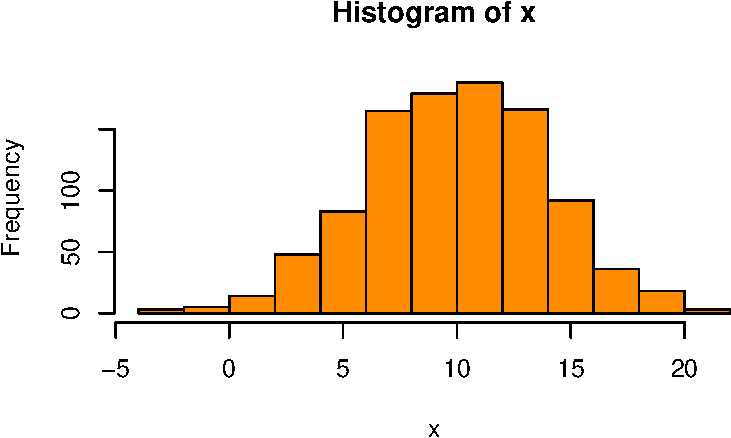
\includegraphics[width=1\linewidth,height=\textheight,keepaspectratio]{dispensa-statistica-descrittiva_files/figure-pdf/fig-hist-1.pdf}

}

\subcaption{\label{fig-hist-1}hist(x)}

\end{minipage}%
%
\begin{minipage}{0.33\linewidth}

\centering{

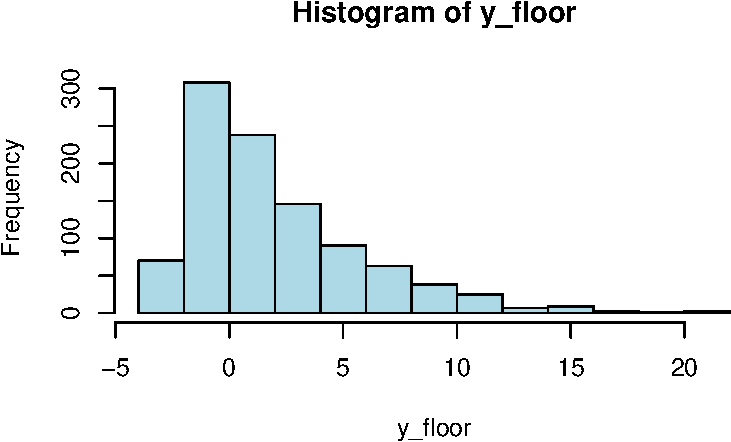
\includegraphics[width=1\linewidth,height=\textheight,keepaspectratio]{dispensa-statistica-descrittiva_files/figure-pdf/fig-hist-2.pdf}

}

\subcaption{\label{fig-hist-2}hist(y)}

\end{minipage}%
%
\begin{minipage}{0.33\linewidth}

\centering{

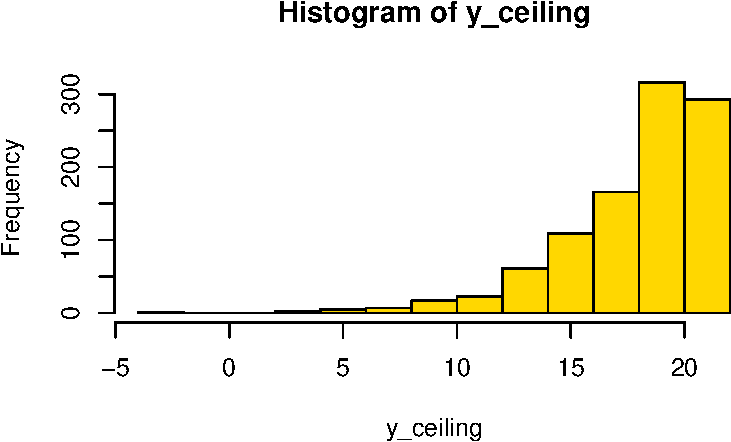
\includegraphics[width=1\linewidth,height=\textheight,keepaspectratio]{dispensa-statistica-descrittiva_files/figure-pdf/fig-hist-3.pdf}

}

\subcaption{\label{fig-hist-3}hist(z)}

\end{minipage}%

\caption{\label{fig-hist}Distribuzioni a confronto - Le stesse dei
boxplot}

\end{figure}%

\subsection{Confronto boxplot vs
istogramma}\label{confronto-boxplot-vs-istogramma}

\begin{figure}

\begin{minipage}{0.50\linewidth}

\centering{

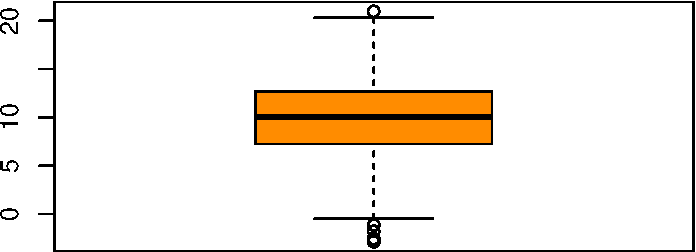
\includegraphics[width=1\linewidth,height=\textheight,keepaspectratio]{dispensa-statistica-descrittiva_files/figure-pdf/fig-comparison0-1.pdf}

}

\subcaption{\label{fig-comparison0-1}boxplot(x)}

\end{minipage}%
%
\begin{minipage}{0.50\linewidth}

\centering{

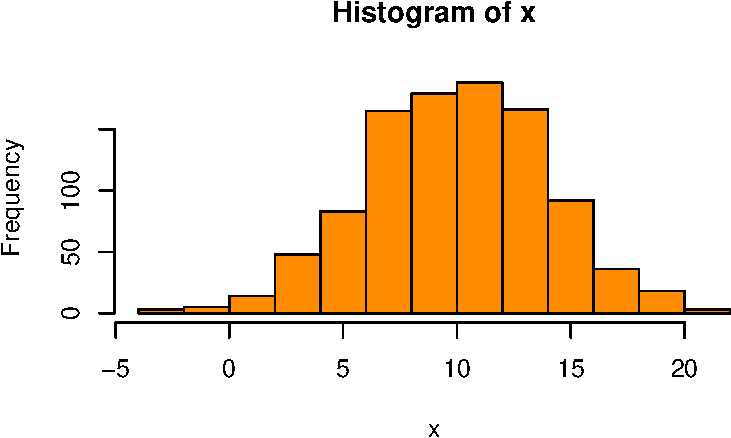
\includegraphics[width=1\linewidth,height=\textheight,keepaspectratio]{dispensa-statistica-descrittiva_files/figure-pdf/fig-comparison0-2.pdf}

}

\subcaption{\label{fig-comparison0-2}hist(x)}

\end{minipage}%
\newline
\begin{minipage}{0.50\linewidth}

\centering{

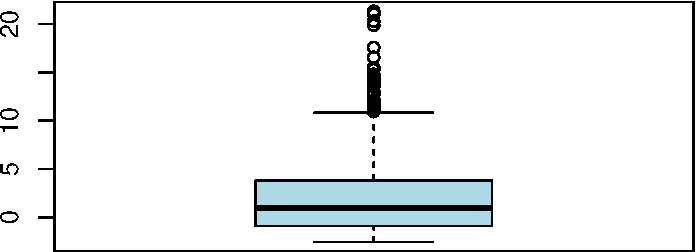
\includegraphics[width=1\linewidth,height=\textheight,keepaspectratio]{dispensa-statistica-descrittiva_files/figure-pdf/fig-comparison0-3.pdf}

}

\subcaption{\label{fig-comparison0-3}boxplot(x)}

\end{minipage}%
%
\begin{minipage}{0.50\linewidth}

\centering{

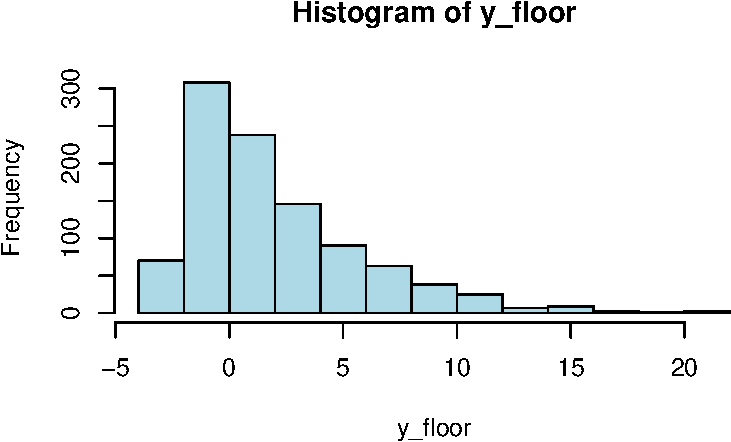
\includegraphics[width=1\linewidth,height=\textheight,keepaspectratio]{dispensa-statistica-descrittiva_files/figure-pdf/fig-comparison0-4.pdf}

}

\subcaption{\label{fig-comparison0-4}hist(x)}

\end{minipage}%
\newline
\begin{minipage}{0.50\linewidth}

\centering{

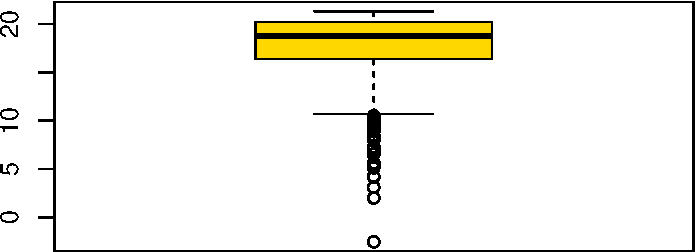
\includegraphics[width=1\linewidth,height=\textheight,keepaspectratio]{dispensa-statistica-descrittiva_files/figure-pdf/fig-comparison0-5.pdf}

}

\subcaption{\label{fig-comparison0-5}boxplot(x)}

\end{minipage}%
%
\begin{minipage}{0.50\linewidth}

\centering{

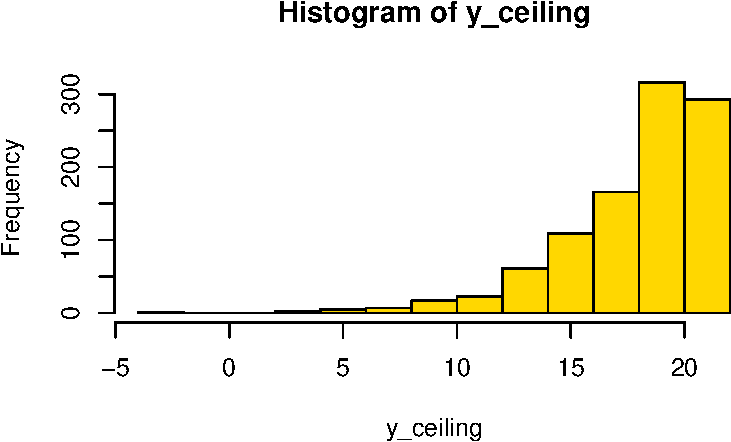
\includegraphics[width=1\linewidth,height=\textheight,keepaspectratio]{dispensa-statistica-descrittiva_files/figure-pdf/fig-comparison0-6.pdf}

}

\subcaption{\label{fig-comparison0-6}hist(x)}

\end{minipage}%

\caption{\label{fig-comparison0}Boxplot vs Istogramma}

\end{figure}%

Forzano i boxpolot ad essere in orizzontale attraverso l'argomento
\texttt{horizontal\ =\ TRUE} (\textbf{?@fig-myFigure}) si può apprezzare
meglio la similutudine tra la forma della distribuzione vista con
l'istogramma e la forma della distribuzione vista con il boxplot.

\begin{figure}

\begin{minipage}{0.33\linewidth}

\centering{

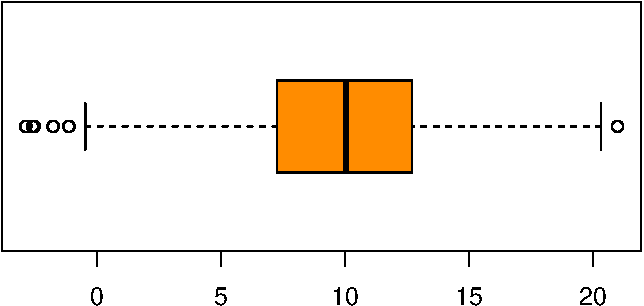
\includegraphics[width=0.7\linewidth,height=\textheight,keepaspectratio]{dispensa-statistica-descrittiva_files/figure-pdf/fig-myfigure-1.pdf}

}

\subcaption{\label{fig-myfigure-1}}

\end{minipage}%
%
\begin{minipage}{0.33\linewidth}

\centering{

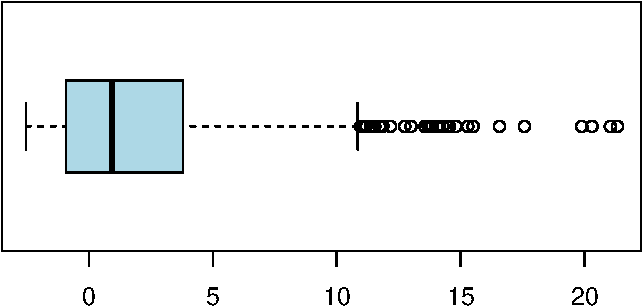
\includegraphics[width=0.7\linewidth,height=\textheight,keepaspectratio]{dispensa-statistica-descrittiva_files/figure-pdf/fig-myfigure-2.pdf}

}

\subcaption{\label{fig-myfigure-2}}

\end{minipage}%
%
\begin{minipage}{0.33\linewidth}

\centering{

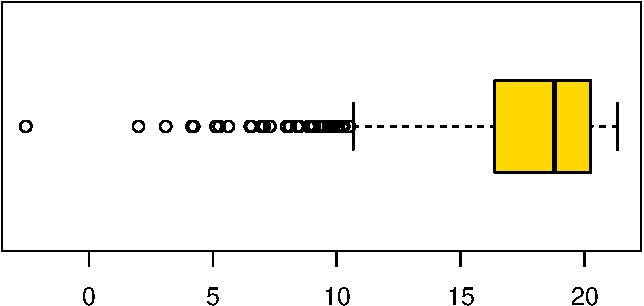
\includegraphics[width=0.7\linewidth,height=\textheight,keepaspectratio]{dispensa-statistica-descrittiva_files/figure-pdf/fig-myfigure-3.pdf}

}

\subcaption{\label{fig-myfigure-3}}

\end{minipage}%
\newline
\begin{minipage}{0.33\linewidth}

\centering{

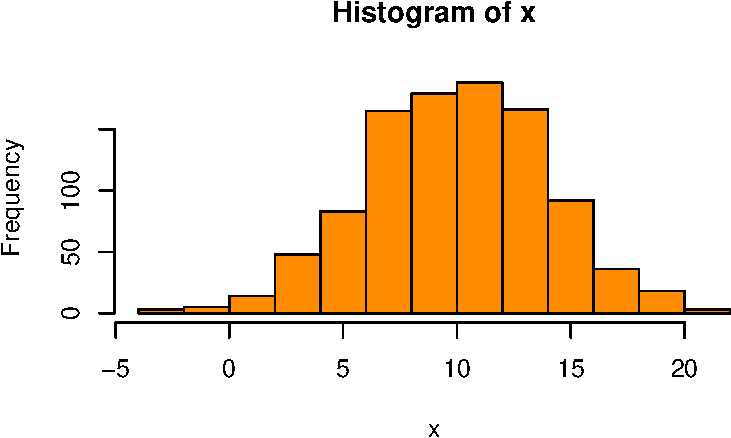
\includegraphics[width=0.7\linewidth,height=\textheight,keepaspectratio]{dispensa-statistica-descrittiva_files/figure-pdf/fig-myfigure-4.pdf}

}

\subcaption{\label{fig-myfigure-4}}

\end{minipage}%
%
\begin{minipage}{0.33\linewidth}

\centering{

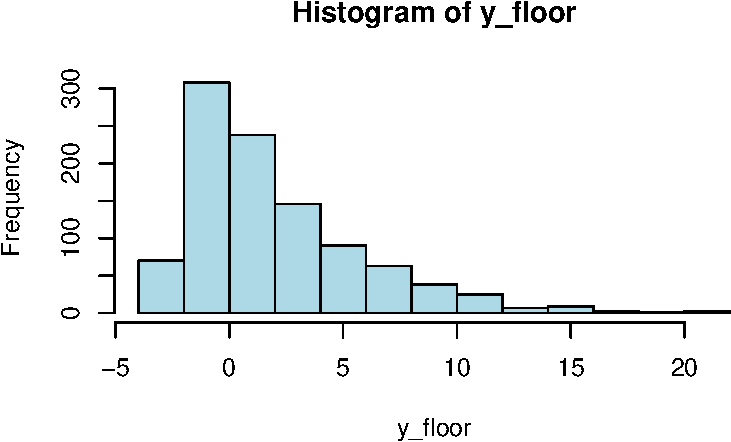
\includegraphics[width=0.7\linewidth,height=\textheight,keepaspectratio]{dispensa-statistica-descrittiva_files/figure-pdf/fig-myfigure-5.pdf}

}

\subcaption{\label{fig-myfigure-5}}

\end{minipage}%
%
\begin{minipage}{0.33\linewidth}

\centering{

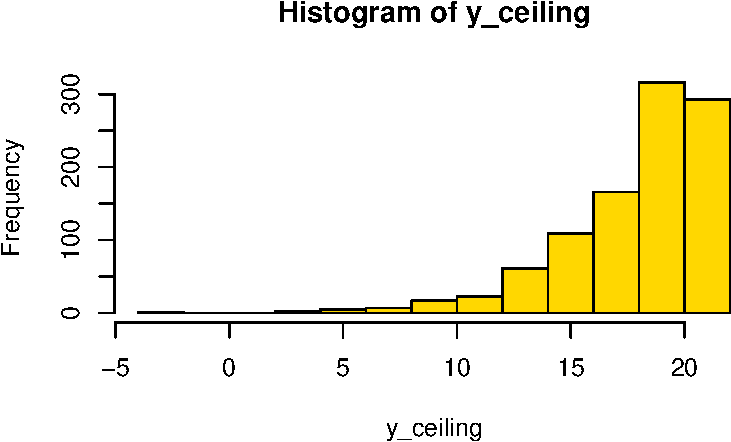
\includegraphics[width=0.7\linewidth,height=\textheight,keepaspectratio]{dispensa-statistica-descrittiva_files/figure-pdf/fig-myfigure-6.pdf}

}

\subcaption{\label{fig-myfigure-6}}

\end{minipage}%

\end{figure}%

Figure~\ref{fig-boxMulti} illustra gli stessi boxplot disposti nella
stessa finestra (Listing~\ref{lst-box}).

\begin{codelisting}

\caption{\label{lst-box}Finestra grafica con molti boxplot}

\centering{

\begin{Shaded}
\begin{Highlighting}[]
\FunctionTok{boxplot}\NormalTok{(x, y, z, }
        \AttributeTok{names =} \FunctionTok{c}\NormalTok{(}\StringTok{"Normale"}\NormalTok{, }\StringTok{"Pavimento"}\NormalTok{, }\StringTok{"Soffitto"}\NormalTok{), }
        \AttributeTok{col =} \FunctionTok{c}\NormalTok{(}\StringTok{"darkorange"}\NormalTok{, }\StringTok{"lightblue"}\NormalTok{, }\StringTok{"gold"}\NormalTok{))}
\end{Highlighting}
\end{Shaded}

}

\end{codelisting}%

\begin{figure}[H]

\centering{

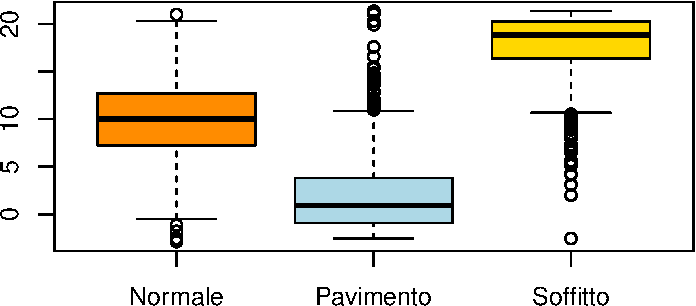
\includegraphics[width=0.7\linewidth,height=\textheight,keepaspectratio]{dispensa-statistica-descrittiva_files/figure-pdf/fig-boxMulti-1.pdf}

}

\caption{\label{fig-boxMulti}Tanti boxplot in un unico grafico}

\end{figure}%

\chapter{Modulo 3 -- Statistica descrittiva
bivariata}\label{modulo-3-statistica-descrittiva-bivariata}

\section{Variabile statistica doppia}\label{variabile-statistica-doppia}

Si consideri un gruppo di 11 persone, per ciascuna delle quali sono
state rilevate due variabili categoriali: il titolo di studio (\(X\),
con categorie Elementare, Secondaria Inferiore e Secondaria Superiore) e
l'occupazione (\(Y\), con categorie Disoccupato, Impiegato e Dirigente).
I dati sono riportati in Table~\ref{tbl-dati-doppia}.

\begin{table}

\caption{\label{tbl-dati-doppia}Titolo di studio e occupazione rilevati su 11 persone}

\centering{

\centering


\begin{tabular}{|c|c|c|c|c|c|c|c|c|c|c|c|}
\hline
$X$: Istruzione & E & E & E & SI & SI & SI & SS & SS & SS & SS & SS\\
\hline
$Y$: Occupazione & DI & I & I & DI & I & I & D & I & I & D & D\\
\hline
\end{tabular}

}

\end{table}%

Ciascuna delle due variabili può essere descritta separatamente
attraverso la sua distribuzione di frequenza. Table~\ref{tbl-freq-x}
riporta le frequenze del titolo di studio (\(n_{k.}\), il numero di
persone che possiedono la categoria \(x_k\)), mentre
Table~\ref{tbl-freq-y} riporta quelle dell'occupazione (\(n_{.j}\), il
numero di persone che possiedono la categoria \(y_j\)).

\begin{table}

\caption{\label{tbl-freq-x}Distribuzioni di frequenza univariate.}

\centering{

\subcaption{\label{tbl-freq-y}Variabile Istruzione}

\centering{

\centering

\begin{minipage}[t]{0.48\textwidth}
\centering


\begin{tabular}{l c}
\hline
categoria $x_k$ & $n_{k.}$\\
\hline
Elementare (E) & \textcolor{red}{3} \\
Secondaria Inferiore (SI) & \textcolor{red}{3}\\
Secondaria Superiore (SS) & \textcolor{red}{5} \\
\hline
\end{tabular}
\end{minipage}\hfill
\begin{minipage}[t]{0.48\textwidth}
\centering
\caption{Variabile Occupazione}

\begin{tabular}{l c}
\hline
categoria $y_j$ & $n_{.j}$ \\
\hline
Disoccupato (DI) & \textcolor{blue}{2} \\
Impiegato (I) & \textcolor{blue}{6}\\
Dirigente (D) & \textcolor{blue}{3} \\
\hline
\end{tabular}
\end{minipage}

}

}

\end{table}%

Le distribuzioni univariate non dicono nulla su come le due variabili si
combinano tra loro: sappiamo quante persone hanno un titolo di studio
elementare e quante sono dirigenti, ma non quante persone con un titolo
elementare sono dirigenti. Per rispondere a questa domanda bisogna
considerare le due variabili \emph{congiuntamente}, contando quante
persone presentano ciascuna coppia di categorie \((x_k, y_j)\). Il
risultato è la \textbf{tabella a doppia entrata} (o tavola di
contingenza) in Table~\ref{tbl-doppia-entrata}: le righe corrispondono
alle categorie di \(X\), le colonne alle categorie di \(Y\), e ogni
cella contiene la \textbf{frequenza congiunta} \(n_{kj}\), cioè il
numero di persone che possiedono contemporaneamente la categoria \(x_k\)
e la categoria \(y_j\).

\begin{table}

\caption{\label{tbl-doppia-entrata}Tabella a doppia entrata di Istruzione e Occupazione}

\centering{

\centering


\begin{tabular}{|c|c|c|c|c|}
\hline
 & DI & I & D & \\
\hline
E  & 1 & 2 & 0 & \textcolor{red}{3}\\
SI & 1 & 2 & 0 & \textcolor{red}{3}\\
SS & 0 & 2 & 3 & \textcolor{red}{5}\\
\hline
 & \textcolor{blue}{2} & \textcolor{blue}{6} & \textcolor{blue}{3} & \textbf{11}\\
\hline
\end{tabular}

}

\end{table}%

Ad esempio, la cella all'incrocio tra la riga SS e la colonna D indica
che 3 persone hanno un titolo di studio di secondaria superiore \emph{e}
sono dirigenti.

Sommando le frequenze congiunte lungo ciascuna riga si ottengono i
totali di riga (in rosso), mentre sommandole lungo ciascuna colonna si
ottengono i totali di colonna (in blu). Questi totali sono detti
\textbf{frequenze marginali}, perché si trovano ai margini della
tabella. Confrontando Table~\ref{tbl-doppia-entrata} con
Table~\ref{tbl-freq-x} e Table~\ref{tbl-freq-y} si nota che le frequenze
marginali di riga coincidono esattamente con la distribuzione di
frequenza di \(X\) e le frequenze marginali di colonna coincidono con la
distribuzione di frequenza di \(Y\). In altre parole, la tabella a
doppia entrata contiene al suo interno anche le due distribuzioni
univariate. Infine, la cella in basso a destra (11) riporta il numero
totale di unità statistiche \(n\), che si ottiene sia sommando i totali
di riga sia sommando i totali di colonna.

Più in generale, date due variabili \(X\) e \(Y\), la loro distribuzione
di frequenze congiunte \(n_{kj}\) descrive quante unità statistiche
presentano ciascuna coppia di categorie \((x_k, y_j)\).

\begin{tcolorbox}[enhanced jigsaw, toprule=.15mm, left=2mm, leftrule=.75mm, breakable, coltitle=black, title={Tip}, bottomtitle=1mm, opacitybacktitle=0.6, toptitle=1mm, titlerule=0mm, bottomrule=.15mm, colframe=quarto-callout-tip-color-frame, arc=.35mm, rightrule=.15mm, opacityback=0, colbacktitle=quarto-callout-tip-color!10!white, colback=white]

L'insieme \((X,Y)\) delle terne

\[(x_k,y_j,n_{kj})
\qquad
(k=1,\ldots,h;\ j=1,\ldots,m)\]

è detto \textbf{variabile statistica doppia}.

\end{tcolorbox}

\subsection{Tabella a doppia entrata -- Tavola di
contingenza}\label{tabella-a-doppia-entrata-tavola-di-contingenza}

\begin{center}
\begin{tabular}{
p{0.7cm} p{0.7cm} |
p{0.7cm} p{0.7cm} p{0.7cm} p{0.7cm} p{0.7cm} p{0.7cm} |
p{0.7cm}
}

& \multicolumn{1}{l}{} 
& \multicolumn{6}{c}{Y} 
& \multicolumn{1}{c}{} \\

& \multicolumn{1}{c}{}
& \multicolumn{1}{l}{$y_1$}
& \multicolumn{1}{l}{$y_2$}
& \multicolumn{1}{l}{$\ldots$}
& \multicolumn{1}{l}{$y_j$}
& \multicolumn{1}{l}{$\ldots$}
& \multicolumn{1}{l}{$y_m$}
& \multicolumn{1}{l}{$n_{k.}$} \\

\cline{3-8}

\multirow{6}{*}{X}

& $x_1$
& $n_{11}$
& $n_{12}$
& $\ldots$
& $n_{1j}$
& $\ldots$
& $n_{1m}$
& $n_{1.}$ \\

& $x_2$
& $n_{21}$
& $n_{22}$
& $\ldots$
& $n_{2j}$
& $\ldots$
& $n_{2m}$
& $n_{2.}$ \\

& $\vdots$
& $\vdots$
& $\vdots$
& 
& $\vdots$
& 
& $\vdots$
& $\vdots$ \\

& $x_k$
& $n_{k1}$
& $n_{k2}$
& $\ldots$
& $n_{kj}$
& $\ldots$
& $n_{km}$
& $n_{k.}$ \\

& $\vdots$
& $\vdots$
& $\vdots$
&
& $\vdots$
&
& $\vdots$
& $\vdots$ \\

& $x_h$
& $n_{h1}$
& $n_{h2}$
& $\ldots$
& $n_{hj}$
& $\ldots$
& $n_{hm}$
& $n_{h.}$ \\

\cline{3-8}

&
& $n_{.1}$
& $n_{.2}$
& $\ldots$
& $n_{.j}$
& $\ldots$
& $n_{.m}$
& $n$ \\

\end{tabular}
\end{center}

\(n_{kj}\): \textbf{Frequenza congiunta}, definisce il numero di unità
statistiche che possiedono congiuntamente la categoria \(x_k\) della
variabile \(X\) e la categoria \(y_j\) della variabile \(Y\)

\(n_{k.}\): \textbf{Frequenza marginale di \(X\)}, definisce il numero
di unità statistiche che possiedono la categoria \(x_k\) della variabile
\(X\)

\(n_{.j}\): \textbf{Frequenza marginale di \(Y\)}, definisce il numero
di unità statistiche che possiedono la categoria \(y_j\) della variabile
\(Y\)

\(n\): Numero totale di unità statistiche

\begin{center}
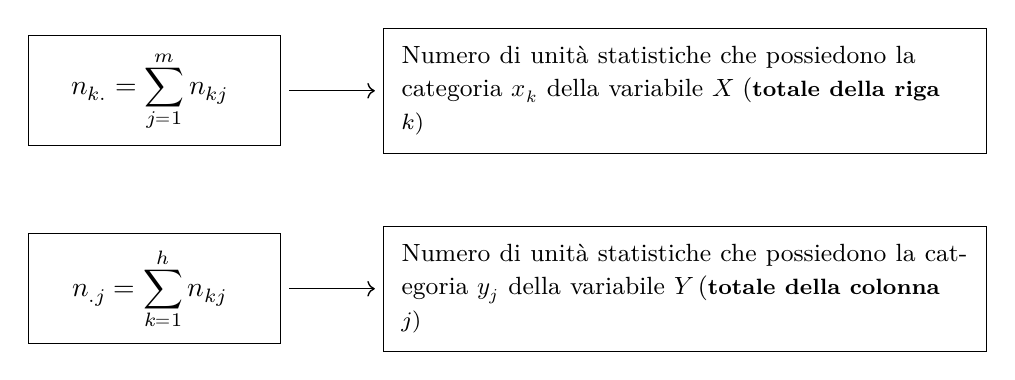
\begin{tikzpicture}[
    node distance=1.1cm and 1.3cm,
    formula/.style={
        draw,
        fill=white,
        minimum width=3.2cm,
        minimum height=1.4cm,
        align=center,
        inner sep=1ex
    },
    description/.style={
        draw,
        fill=white,
        text width=7.2cm,
        minimum height=1.4cm,
        align=left,
        inner sep=1.5ex
    },
    arrow/.style={
        ->,
        line width=0.5pt,
        shorten >=3pt,
        shorten <=3pt
    }
]

% Frequenza marginale di X
\node[formula] (A) {
    $\displaystyle n_{k.} = \sum_{j=1}^{m} n_{kj}$
};

\node[description, right=of A] (C) {
  \small  Numero di unità statistiche che possiedono la
    categoria $x_k$ della variabile $X$
    (\footnotesize \textbf{totale della riga $k$})
};

\draw[arrow] (A) -- (C);

% Frequenza marginale di Y
\node[formula, below=of A] (D) {
    $\displaystyle n_{.j} = \sum_{k=1}^{h} n_{kj}$
};

\node[description, right=of D] (E) {
    \small Numero di unità statistiche che possiedono la
    categoria $y_j$ della variabile $Y$
    (\footnotesize  \textbf{totale della colonna $j$})
};

\draw[arrow] (D) -- (E);

\end{tikzpicture}
\end{center}

\[
\sum_{k=1}^{h}\sum_{j=1}^{m} n_{kj}
=
\sum_{k=1}^{h} n_{k.}
=
\sum_{j=1}^{m} n_{.j}
=
n
\]

\subsection{\texorpdfstring{\texttt{table()}}{table()}}\label{table}

\texttt{table(var1,\ var2)}: Produce la tabella di frequenza tra due
variabili categoriali \texttt{var1} e \texttt{var2}

\begin{Shaded}
\begin{Highlighting}[]
\NormalTok{var1 }\OtherTok{\textless{}{-}} \FunctionTok{as.factor}\NormalTok{(}\FunctionTok{c}\NormalTok{(}\StringTok{"a1"}\NormalTok{,}\StringTok{"a2"}\NormalTok{,}\StringTok{"a1"}\NormalTok{,}\StringTok{"a2"}\NormalTok{,}\StringTok{"a1"}\NormalTok{,}\StringTok{"a2"}\NormalTok{,}\StringTok{"a1"}\NormalTok{))  }
\NormalTok{var2 }\OtherTok{\textless{}{-}} \FunctionTok{as.factor}\NormalTok{(}\FunctionTok{c}\NormalTok{(}\StringTok{"b1"}\NormalTok{,}\StringTok{"b1"}\NormalTok{,}\StringTok{"b1"}\NormalTok{,}\StringTok{"b2"}\NormalTok{,}\StringTok{"b1"}\NormalTok{,}\StringTok{"b2"}\NormalTok{,}\StringTok{"b2"}\NormalTok{)) }
\NormalTok{mytab }\OtherTok{=} \FunctionTok{table}\NormalTok{(var1, var2); mytab}
\end{Highlighting}
\end{Shaded}

\begin{verbatim}
    var2
var1 b1 b2
  a1  3  1
  a2  1  2
\end{verbatim}

\begin{Shaded}
\begin{Highlighting}[]
\FunctionTok{sum}\NormalTok{(mytab) }\CommentTok{\# permette di ottenere l\textquotesingle{}ampiezza campionaria}
\end{Highlighting}
\end{Shaded}

\begin{verbatim}
[1] 7
\end{verbatim}

\subsection{\texorpdfstring{\texttt{margin.table()}}{margin.table()}}\label{margin.table}

\texttt{margin.table(table,\ margin)}: Frequenze marginali per la
tabella a doppia entrata

\begin{tcolorbox}[enhanced jigsaw, toprule=.15mm, left=2mm, leftrule=.75mm, breakable, coltitle=black, title={Tip}, bottomtitle=1mm, opacitybacktitle=0.6, toptitle=1mm, titlerule=0mm, bottomrule=.15mm, colframe=quarto-callout-tip-color-frame, arc=.35mm, rightrule=.15mm, opacityback=0, colbacktitle=quarto-callout-tip-color!10!white, colback=white]

\texttt{margin\ =\ 1}: Frequenze marginali calcolate \textbf{attraverso
le colonne}

\texttt{margin\ =\ 2}: Frequenze marginali calcolate \textbf{attraverso
le righe}

\end{tcolorbox}

\begin{Shaded}
\begin{Highlighting}[]
\NormalTok{mytab}
\end{Highlighting}
\end{Shaded}

\begin{verbatim}
    var2
var1 b1 b2
  a1  3  1
  a2  1  2
\end{verbatim}

\begin{Shaded}
\begin{Highlighting}[]
\FunctionTok{margin.table}\NormalTok{(mytab,}\DecValTok{1}\NormalTok{)  }
\end{Highlighting}
\end{Shaded}

\begin{verbatim}
var1
a1 a2 
 4  3 
\end{verbatim}

\begin{Shaded}
\begin{Highlighting}[]
\FunctionTok{margin.table}\NormalTok{(mytab,}\DecValTok{2}\NormalTok{)  }
\end{Highlighting}
\end{Shaded}

\begin{verbatim}
var2
b1 b2 
 4  3 
\end{verbatim}

\subsection{\texorpdfstring{\texttt{prop.table()}}{prop.table()}}\label{prop.table}

\texttt{prop.table(T,\ margin\ =\ NULL)}: Probabilità condizionate:

\begin{tcolorbox}[enhanced jigsaw, toprule=.15mm, left=2mm, leftrule=.75mm, breakable, coltitle=black, title={Tip}, bottomtitle=1mm, opacitybacktitle=0.6, toptitle=1mm, titlerule=0mm, bottomrule=.15mm, colframe=quarto-callout-tip-color-frame, arc=.35mm, rightrule=.15mm, opacityback=0, colbacktitle=quarto-callout-tip-color!10!white, colback=white]

\texttt{margin\ =\ 1}: Probabilità calcolate sul totale \(n\),
\(p_{kj} = \dfrac{n_{kj}}{n}\)

\texttt{margin\ =\ 1}: Probabilità condizionate di riga
(\textbf{attraverso le colonne}), \(p_{kj} = \dfrac{n_{kj}}{n_{k.}}\)

\texttt{margin\ =\ 2}: Probabilità condizionate di colonna
(\textbf{attraverso le righe}), \(p_{kj} = \dfrac{n_{kj}}{n_{.j}}\)

\end{tcolorbox}

\begin{Shaded}
\begin{Highlighting}[]
\NormalTok{mytab}
\end{Highlighting}
\end{Shaded}

\begin{verbatim}
    var2
var1 b1 b2
  a1  3  1
  a2  1  2
\end{verbatim}

\begin{Shaded}
\begin{Highlighting}[]
\FunctionTok{prop.table}\NormalTok{(mytab)   }
\end{Highlighting}
\end{Shaded}

\begin{verbatim}
    var2
var1        b1        b2
  a1 0.4285714 0.1428571
  a2 0.1428571 0.2857143
\end{verbatim}

\begin{Shaded}
\begin{Highlighting}[]
\FunctionTok{prop.table}\NormalTok{(mytab,}\DecValTok{1}\NormalTok{)  }\CommentTok{\# P(B|A)}
\end{Highlighting}
\end{Shaded}

\begin{verbatim}
    var2
var1        b1        b2
  a1 0.7500000 0.2500000
  a2 0.3333333 0.6666667
\end{verbatim}

\begin{Shaded}
\begin{Highlighting}[]
\FunctionTok{prop.table}\NormalTok{(mytab,}\DecValTok{2}\NormalTok{)  }\CommentTok{\# P(A|B)}
\end{Highlighting}
\end{Shaded}

\begin{verbatim}
    var2
var1        b1        b2
  a1 0.7500000 0.3333333
  a2 0.2500000 0.6666667
\end{verbatim}

\subsection{Frequenze percentuali e frequenze
condizionate}\label{frequenze-percentuali-e-frequenze-condizionate}

Si consideri un campione di 140 donne per le quali sono state rilevate
due variabili categoriali: l'occupazione (casalinga o lavoratrice) e il
livello di istruzione (basso, medio o alto). La tabella a doppia entrata
con le frequenze assolute e le marginali è riportata in
Table~\ref{tbl-donne-contingenza}.

\begin{longtable}[t]{lcccc}

\caption{\label{tbl-donne-contingenza}Tabella a doppia entrata di
Occupazione e Istruzione (frequenze assolute)}

\tabularnewline

\toprule
 & Basso & Medio & Alto & Totale\\
\midrule
Casalinghe & 40 & 25 & 20 & 85\\
Lavoratrici & 10 & 15 & 30 & 55\\
\midrule\\
Totale & 50 & 40 & 50 & 140\\
\bottomrule

\end{longtable}

Guardando le frequenze assolute si potrebbe essere tentati di
concludere, ad esempio, che tra le donne con istruzione alta ci sono più
lavoratrici (30) che casalinghe (20), e che tra quelle con istruzione
bassa ci sono molte più casalinghe (40) che lavoratrici (10). Le
frequenze assolute, però, non permettono confronti corretti, perché i
gruppi hanno dimensioni diverse: nel campione ci sono 85 casalinghe e
solo 55 lavoratrici, e anche i tre livelli di istruzione non hanno la
stessa numerosità (50, 40 e 50). Un numero più alto in una cella può
dipendere semplicemente dal fatto che quel gruppo è più numeroso.

Per confrontare gruppi di dimensione diversa bisogna passare alle
\textbf{frequenze percentuali condizionate}: invece di dividere ogni
cella per il totale generale \(n\) (quelo che fa la funzione
\texttt{prop.table(tabella)} quando non viene specificato un margin), la
si divide per il totale della sua riga o della sua colonna. In questo
modo ogni riga (o ogni colonna) diventa una distribuzione percentuale
che somma a 100, e i gruppi diventano confrontabili.

La stessa tabella si può leggere in due modi diversi, a seconda di quale
variabile si sceglie come \emph{condizionante}, cioè di quale variabile
si fissano le categorie per guardare come si distribuisce l'altra.

Un primo colpo d'occhio sulla struttura della tabella è dato dal mosaic
plot in Figure~\ref{fig-donne-mosaic}. La larghezza delle due colonne è
proporzionale al numero di casalinghe e di lavoratrici, mentre l'altezza
dei rettangoli all'interno di ciascuna colonna rappresenta la
percentuale di donne con istruzione bassa, media o alta \emph{in quel
gruppo}.

\begin{figure}

\centering{

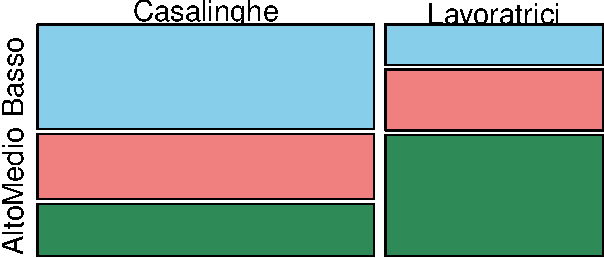
\includegraphics[width=0.6\linewidth,height=\textheight,keepaspectratio]{dispensa-statistica-descrittiva_files/figure-pdf/fig-donne-mosaic-1.pdf}

}

\caption{\label{fig-donne-mosaic}Mosaic plot di Occupazione e
Istruzione}

\end{figure}%

\subsubsection{\texorpdfstring{Frequenze percentuali di riga:
\(P(\text{Istruzione} \mid \text{Occupazione})\)}{Frequenze percentuali di riga: P(\textbackslash text\{Istruzione\} \textbackslash mid \textbackslash text\{Occupazione\})}}\label{frequenze-percentuali-di-riga-ptextistruzione-mid-textoccupazione}

Le percentuali di \textbf{riga} si ottengono dividendo ogni cella per il
totale della propria riga (\texttt{prop.table(tabella,\ 1)}). Poiché le
righe corrispondono all'occupazione, ogni riga descrive \emph{come si
distribuisce il titolo di studio all'interno di ciascun gruppo
occupazionale} (Table~\ref{tbl-donne-perc-riga} e
Figure~\ref{fig-donne-perc-riga}).

\begin{longtable}[]{@{}lcccc@{}}

\caption{\label{tbl-donne-perc-riga}Frequenze percentuali di riga:
distribuzione dell'Istruzione condizionata all'Occupazione}

\tabularnewline

\toprule\noalign{}
& Basso & Medio & Alto & Totale \\
\midrule\noalign{}
\endhead
\bottomrule\noalign{}
\endlastfoot
Casalinghe & 47 & 29 & 24 & 100 \\
Lavoratrici & 18 & 27 & 55 & 100 \\

\end{longtable}

\begin{figure}

\centering{

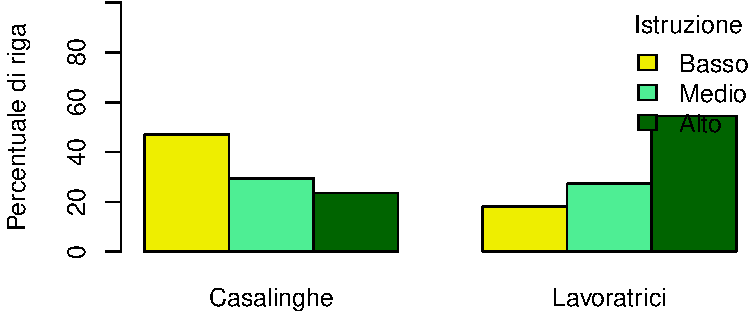
\includegraphics[width=0.7\linewidth,height=\textheight,keepaspectratio]{dispensa-statistica-descrittiva_files/figure-pdf/fig-donne-perc-riga-1.pdf}

}

\caption{\label{fig-donne-perc-riga}Distribuzione percentuale
dell'Istruzione nei due gruppi occupazionali}

\end{figure}%

La lettura corretta è sempre del tipo \emph{``tra le donne {[}categoria
di occupazione{]}, il X\% ha un titolo di studio {[}categoria di
istruzione{]}''}. Ad esempio:

\begin{itemize}
\tightlist
\item
  tra le casalinghe, il 47\% ha un titolo di studio basso e solo il 24\%
  un titolo alto;
\item
  tra le lavoratrici, il 55\% ha un titolo di studio alto e solo il 18\%
  un titolo basso.
\end{itemize}

Le percentuali di riga descrivono quindi la \textbf{composizione} di
ciascun gruppo occupazionale: rispondono a domande del tipo \emph{``che
titolo di studio hanno le casalinghe?''}.

\subsubsection{\texorpdfstring{Frequenze percentuali di colonna:
\(P(\text{Occupazione} \mid \text{Istruzione})\)}{Frequenze percentuali di colonna: P(\textbackslash text\{Occupazione\} \textbackslash mid \textbackslash text\{Istruzione\})}}\label{frequenze-percentuali-di-colonna-ptextoccupazione-mid-textistruzione}

Le percentuali di \textbf{colonna} si ottengono dividendo ogni cella per
il totale della propria colonna (\texttt{prop.table(tabella,\ 2)}).
Poiché le colonne corrispondono al titolo di studio, ogni colonna
descrive \emph{come si distribuisce l'occupazione all'interno di ciascun
livello di istruzione} (Table~\ref{tbl-donne-perc-colonna} e
Figure~\ref{fig-donne-perc-colonna}).

\begin{longtable}[]{@{}lccc@{}}

\caption{\label{tbl-donne-perc-colonna}Frequenze percentuali di colonna:
distribuzione dell'Occupazione condizionata all'Istruzione}

\tabularnewline

\toprule\noalign{}
& Basso & Medio & Alto \\
\midrule\noalign{}
\endhead
\bottomrule\noalign{}
\endlastfoot
Casalinghe & 80 & 62 & 40 \\
Lavoratrici & 20 & 38 & 60 \\
Totale & 100 & 100 & 100 \\

\end{longtable}

\begin{figure}

\centering{

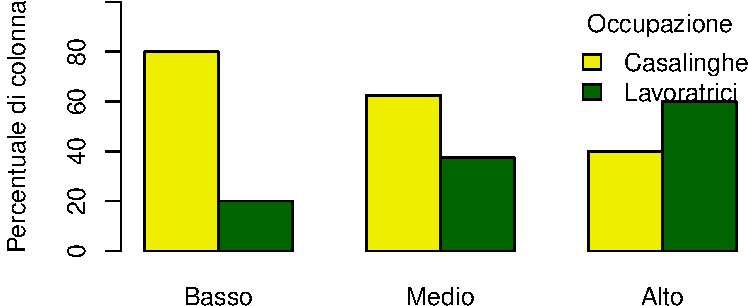
\includegraphics[width=0.7\linewidth,height=\textheight,keepaspectratio]{dispensa-statistica-descrittiva_files/figure-pdf/fig-donne-perc-colonna-1.pdf}

}

\caption{\label{fig-donne-perc-colonna}Distribuzione percentuale
dell'Occupazione nei tre livelli di istruzione}

\end{figure}%

In questo caso la lettura è del tipo \emph{``tra le donne con titolo di
studio {[}categoria di istruzione{]}, il X\% è {[}categoria di
occupazione{]}''}. Ad esempio:

\begin{itemize}
\tightlist
\item
  tra le donne con titolo di studio basso, l'80\% è casalinga e solo il
  20\% lavora;
\item
  tra le donne con titolo di studio alto, la situazione si capovolge: il
  60\% lavora e il 40\% è casalinga.
\end{itemize}

Al crescere del titolo di studio, quindi, cresce la percentuale di
lavoratrici (20\%, 38\%, 60\%).

\subsubsection{Quale percentuale ha senso
calcolare?}\label{quale-percentuale-ha-senso-calcolare}

Dal punto di vista del calcolo, entrambe le percentuali sono sempre
ottenibili, e R le restituisce senza alcun problema. La scelta di quale
usare dipende dalla \textbf{domanda di ricerca}, cioè da quale variabile
ha senso considerare come condizionante e quale come variabile da
descrivere.

In questo esempio è più naturale ragionare in termini di
\(P(\text{Occupazione} \mid \text{Istruzione})\), cioè con le
percentuali di \textbf{colonna}. Il titolo di studio, infatti, si
acquisisce di norma \emph{prima} di entrare nel mondo del lavoro: ha
senso chiedersi se e come l'occupazione cambi al variare del titolo di
studio, mentre ha molto meno senso pensare che essere casalinga o
lavoratrice determini il titolo di studio posseduto. Le percentuali di
riga restano comunque utili a scopo descrittivo (per sapere, ad esempio,
com'è composto il gruppo delle casalinghe), ma non vanno lette come se
l'occupazione ``spiegasse'' l'istruzione.

\begin{tcolorbox}[enhanced jigsaw, toprule=.15mm, left=2mm, leftrule=.75mm, breakable, coltitle=black, title={Una regola pratica}, bottomtitle=1mm, opacitybacktitle=0.6, toptitle=1mm, titlerule=0mm, bottomrule=.15mm, colframe=quarto-callout-tip-color-frame, arc=.35mm, rightrule=.15mm, opacityback=0, colbacktitle=quarto-callout-tip-color!10!white, colback=white]

Si condiziona sulla variabile che si pensa possa \emph{spiegare} o
\emph{precedere} l'altra, e si calcolano le percentuali all'interno
delle sue categorie. Poi si confrontano le percentuali \textbf{tra} le
categorie della variabile condizionante: se le distribuzioni sono
diverse tra loro, le due variabili sono in qualche modo associate.

\end{tcolorbox}

\begin{tcolorbox}[enhanced jigsaw, toprule=.15mm, left=2mm, leftrule=.75mm, breakable, coltitle=black, title={Condizionare non vuol dire dimostrare una causa}, bottomtitle=1mm, opacitybacktitle=0.6, toptitle=1mm, titlerule=0mm, bottomrule=.15mm, colframe=quarto-callout-warning-color-frame, arc=.35mm, rightrule=.15mm, opacityback=0, colbacktitle=quarto-callout-warning-color!10!white, colback=white]

Scegliere una variabile come condizionante è una scelta di lettura dei
dati, non una prova di un legame causale. Che tra le donne con
istruzione alta ci siano più lavoratrici non dimostra che sia il titolo
di studio a \emph{causare} l'occupazione: le due variabili potrebbero
dipendere entrambe da altri fattori, ad esempio la condizione economica
della famiglia di origine.

\end{tcolorbox}

Infine, se le due variabili fossero \textbf{indipendenti}, le
distribuzioni condizionate sarebbero tutte uguali tra loro e uguali alla
distribuzione marginale. In questo caso, ad esempio, in ogni livello di
istruzione ci si aspetterebbe di trovare la stessa percentuale di
lavoratrici osservata nel campione complessivo, cioè
\(55/140 \approx 39\%\). Le percentuali osservate (20\%, 38\% e 60\%)
sono invece molto diverse tra loro: è proprio questa distanza dalla
situazione di indipendenza che l'indice \(\chi^2\), presentato nella
sezione successiva, permette di quantificare.

\section{Connessione (Variabili
qualitative)}\label{connessione-variabili-qualitative}

\begin{center}
La CONNESSIONE tra due variabili categoriali equivale alla NON INDIPENDENZA!
        
\end{center}

Tra le variabili \(X\) e \(Y\) c'è una forma di legame e
\textbf{relazione} (\textbf{connessione}) \(\rightarrow\) il variare di
una implica un qualche cambiamento \textbf{non casuale} nell'altra.

\subsection{\texorpdfstring{\(\chi^2\)}{\textbackslash chi\^{}2}}\label{chi2}

Quantifica la DISTANZA DALL'INDIPENDENZA tra due variabili categoriali.

\begin{itemize}
\tightlist
\item
  X con \(h\) categorie \(x_k\), con \(k=1,\ldots,h\),
\item
  Y con \(m\) categorie \(y_j\), con \(j=1,\ldots,m\)
\end{itemize}

Richiede il confronto tra \textbf{frequenze osservate} (\(n_{kj}\)) e
\textbf{frequenze attese} o \textbf{frequenze teoriche} (\(n_{kj}^*\)).

\begin{columns}
\begin{column}{0.40\textwidth}
\begin{tabular}{|p{2.5cm}|p{1cm}|}
\hline
& \\
\multicolumn{1}{|c|}{${n_{kj}}$} & \multicolumn{1}{c|}{$n_{k.}$}\\
& \\
\hline
\multicolumn{1}{|c|}{$n_{.j}$} & \\
\hline
\end{tabular}
    
    
\vspace{3mm}
Frequenze osservate
\end{column}
\begin{column}{0.10\textwidth}
VS.
\end{colum}
\begin{column}{0.50\textwidth}


\begin{tabular}{|p{2.5cm}|p{1cm}|}
\hline
& \\
\multicolumn{1}{|c|}{$n_{kj}^*$} & \multicolumn{1}{c|}{$n_{k.}$}\\
& \\
\hline
\multicolumn{1}{|c|}{$n_{.j}$} & \\
\hline
\end{tabular}

\vspace{3mm}
Frequenze teoriche

\end{colum}

\end{columns}

\begin{tcolorbox}[enhanced jigsaw, toprule=.15mm, left=2mm, leftrule=.75mm, breakable, coltitle=black, title={\(n_{kj}^*\): Significato}, bottomtitle=1mm, opacitybacktitle=0.6, toptitle=1mm, titlerule=0mm, bottomrule=.15mm, colframe=quarto-callout-tip-color-frame, arc=.35mm, rightrule=.15mm, opacityback=0, colbacktitle=quarto-callout-tip-color!10!white, colback=white]

Data l'ampiezza campionaria \(n\), quali sono le frequenze che avremmo
dovuto osservare se le due variabili fossero state indipendenti, ovvero
se non avessero alcuna relazione?

\[n_{kj}^* = \dfrac{n_{k.} \times n_{.j}}{n}, \qquad n = \sum_{k=1}^h \sum_{j=1}^m n_{kj} = \sum_{k=1}^h \sum_{j=1}^m n_{kj}^*\]

\end{tcolorbox}

Siccome le frequenze teoriche sono le frequenze che si sarebbero
osservate se le variabili fossero state indipendeti \textbf{data
l'ampiezza campionaria e i marginali di riga e colonna osservati}, la
somma di tutte le frequenze teoriche restituisce l'ampiezza campionaria
\(n\). Inoltre, i marginali di riga delle frequenze teoriche sono uguali
ai marginali di riga delle frequenze osservate, così come i marginali di
colonna delle frequenze teoriche sono uguali ai marginali di colonna
delle frequenze osservate.

\begin{Shaded}
\begin{Highlighting}[]
\NormalTok{knitr}\SpecialCharTok{::}\FunctionTok{kable}\NormalTok{(tabella,}\AttributeTok{booktabs =} \ConstantTok{TRUE}\NormalTok{,}\AttributeTok{align =} \StringTok{"c"}\NormalTok{)}
\end{Highlighting}
\end{Shaded}

\begin{longtable}[]{@{}lcccc@{}}
\caption{Frequenze osservate}\tabularnewline
\toprule\noalign{}
& Basso & Medio & Alto & Totale \\
\midrule\noalign{}
\endfirsthead
\toprule\noalign{}
& Basso & Medio & Alto & Totale \\
\midrule\noalign{}
\endhead
\bottomrule\noalign{}
\endlastfoot
Casalinghe & 40 & 25 & 20 & 85 \\
Lavoratrici & 10 & 15 & 30 & 55 \\
Totale & 50 & 40 & 50 & 140 \\
\end{longtable}

\begin{table}[h]
\centering
\caption{Frequenze teoriche}
\renewcommand{\arraystretch}{1.8}
\begin{tabular}{lccc|c}
\hline
& Basso & Medio & Alto & Totale \\
\hline

Casalinghe
& $\dfrac{85 \times 50}{140} = 30.36$
& $\dfrac{85 \times 40}{140} = 24.29$
& $\dfrac{85 \times 50}{140} = 30.36$
& 85 \\

Lavoratrici
& $\dfrac{55 \times 50}{140} = 19.64$
& $\dfrac{55 \times 40}{140} = 15.71$
& $\dfrac{55 \times 50}{140} = 19.64$
& 55 \\

\hline

Totale
& 50
& 40
& 50
& \textbf{140} \\

\hline
\end{tabular}
\end{table}

\[\chi^2 = \sum_{k=1}^{h} \sum_{j=1}^{m} \displaystyle \frac{(n_{kj} - n_{kj}^*)^2}{n_{kj}^*}\]

\(\chi^2 = 0\): \(n_{kj} = n_{kj}^*\) Indipendenza stocastica

\(\chi^2 = \chi_{\max}^2\): Relazione di perfetta dipendenza (dove
\(\chi_{\max}^2 = n \times \min[(h-1); (m-1)]\))

\[\tilde{\chi}^2 = \dfrac{\chi^2}{\chi_{\max}^2}\]

\(\tilde{\chi}^2\) è il \(\chi^2\) normalizzato, permette di esprimere
il grado di associazione tra due variabili categoriali secondo una scala
ti tipo \([0, 1]\)

\subsection{\texorpdfstring{\texttt{chisq.test()}}{chisq.test()}}\label{chisq.test}

\texttt{chisq.test(table)\$statistic}: Calcola il \(\chi^2\) osservato a
partire da una tavola di contingenza ottenuta con \texttt{table()}

\begin{Shaded}
\begin{Highlighting}[]
\NormalTok{mytab}
\end{Highlighting}
\end{Shaded}

\begin{verbatim}
    var2
var1 b1 b2
  a1  3  1
  a2  1  2
\end{verbatim}

\begin{Shaded}
\begin{Highlighting}[]
\FunctionTok{chisq.test}\NormalTok{(mytab)}\SpecialCharTok{$}\NormalTok{statistic}
\end{Highlighting}
\end{Shaded}

\begin{verbatim}
X-squared 
 0.109375 
\end{verbatim}

\subsubsection{\texorpdfstring{Calcolo
\(\chi_{max}^2\)}{Calcolo \textbackslash chi\_\{max\}\^{}2}}\label{calcolo-chi_max2}

\begin{Shaded}
\begin{Highlighting}[]
\NormalTok{chiMax }\OtherTok{=} \FunctionTok{sum}\NormalTok{(mytab) }\SpecialCharTok{*} \FunctionTok{min}\NormalTok{(}\FunctionTok{c}\NormalTok{(}\FunctionTok{nrow}\NormalTok{(mytab) }\SpecialCharTok{{-}} \DecValTok{1}\NormalTok{, }\FunctionTok{ncol}\NormalTok{(mytab) }\SpecialCharTok{{-}} \DecValTok{1}\NormalTok{))}
\NormalTok{chiMax}
\end{Highlighting}
\end{Shaded}

\begin{verbatim}
[1] 7
\end{verbatim}

\begin{Shaded}
\begin{Highlighting}[]
\FunctionTok{chisq.test}\NormalTok{(mytab)}\SpecialCharTok{$}\NormalTok{statistic}\SpecialCharTok{/}\NormalTok{chiMax}
\end{Highlighting}
\end{Shaded}

\begin{verbatim}
Warning in chisq.test(mytab): L'approssimazione al Chi-quadrato potrebbe essere
inesatta
\end{verbatim}

\begin{verbatim}
X-squared 
 0.015625 
\end{verbatim}

\section{Indipendenza stocastica e massima
dipendenza}\label{indipendenza-stocastica-e-massima-dipendenza}

\begin{longtable}[]{@{}lrrrr@{}}
\toprule\noalign{}
& adolescenti & giovani & adulti & anziani \\
\midrule\noalign{}
\endhead
\bottomrule\noalign{}
\endlastfoot
mare & 18 & 24 & 30 & 12 \\
monti & 12 & 16 & 20 & 8 \\
città d'arte & 6 & 8 & 10 & 4 \\
\end{longtable}

\begin{center}
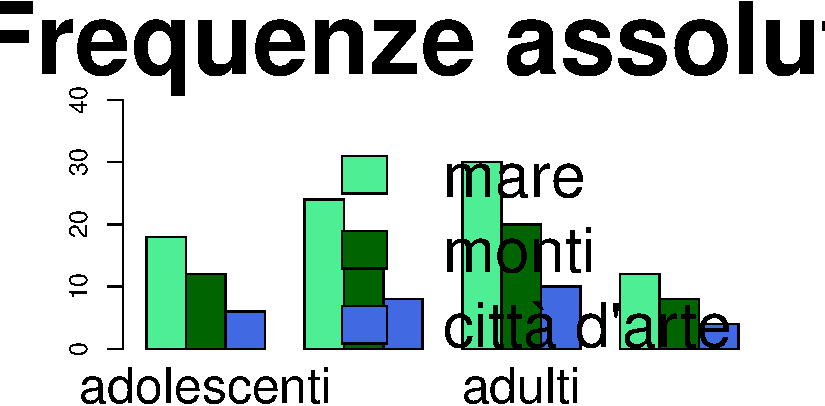
\includegraphics[width=0.5\linewidth,height=\textheight,keepaspectratio]{dispensa-statistica-descrittiva_files/figure-pdf/unnamed-chunk-104-1.pdf}
\end{center}

\begin{figure}

\begin{minipage}{0.50\linewidth}
\begin{center}
\pandocbounded{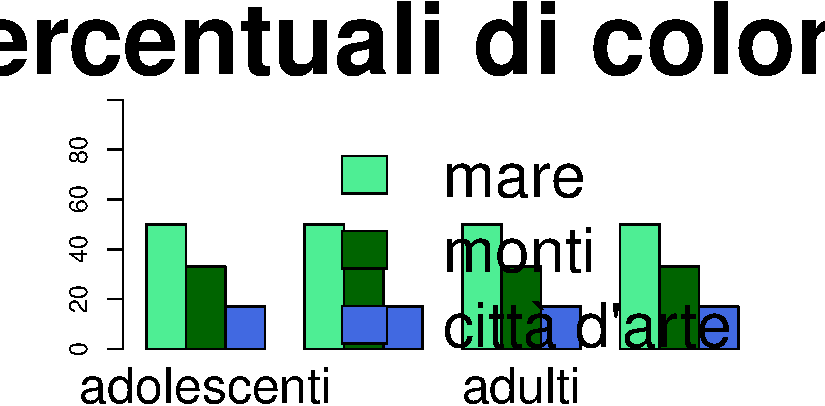
\includegraphics[keepaspectratio]{dispensa-statistica-descrittiva_files/figure-pdf/unnamed-chunk-105-1.pdf}}
\end{center}
\end{minipage}%
%
\begin{minipage}{0.50\linewidth}
\begin{center}
\pandocbounded{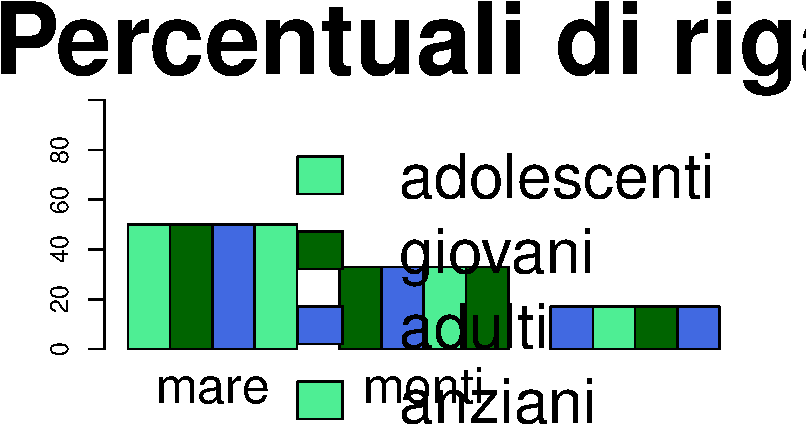
\includegraphics[keepaspectratio]{dispensa-statistica-descrittiva_files/figure-pdf/unnamed-chunk-105-2.pdf}}
\end{center}
\end{minipage}%

\end{figure}%

\textbf{Frequenze osservate}

\begin{Shaded}
\begin{Highlighting}[]
\NormalTok{obs\_n }\OtherTok{=} \FunctionTok{matrix}\NormalTok{(}
  \FunctionTok{c}\NormalTok{(}\DecValTok{18}\NormalTok{, }\DecValTok{24}\NormalTok{, }\DecValTok{30}\NormalTok{, }\DecValTok{12}\NormalTok{,   }\CommentTok{\# mare}
    \DecValTok{12}\NormalTok{, }\DecValTok{16}\NormalTok{, }\DecValTok{20}\NormalTok{, }\DecValTok{8}\NormalTok{,    }\CommentTok{\# monti}
    \DecValTok{6}\NormalTok{, }\DecValTok{8}\NormalTok{, }\DecValTok{10}\NormalTok{, }\DecValTok{4}\NormalTok{),     }\CommentTok{\# città d’arte}
  \AttributeTok{nrow =} \DecValTok{3}\NormalTok{, }\AttributeTok{byrow =} \ConstantTok{TRUE}\NormalTok{) ; obs\_n}
\end{Highlighting}
\end{Shaded}

\begin{verbatim}
     [,1] [,2] [,3] [,4]
[1,]   18   24   30   12
[2,]   12   16   20    8
[3,]    6    8   10    4
\end{verbatim}

\textbf{Frequenze teoriche}

\begin{Shaded}
\begin{Highlighting}[]
\FunctionTok{chisq.test}\NormalTok{(obs\_n)}\SpecialCharTok{$}\NormalTok{expected}
\end{Highlighting}
\end{Shaded}

\begin{verbatim}
     [,1] [,2] [,3] [,4]
[1,]   18   24   30   12
[2,]   12   16   20    8
[3,]    6    8   10    4
\end{verbatim}

\subsubsection{\texorpdfstring{Calcolo
\(\chi^2\)}{Calcolo \textbackslash chi\^{}2}}\label{calcolo-chi2}

\begin{Shaded}
\begin{Highlighting}[]
\FunctionTok{chisq.test}\NormalTok{(obs\_n)}\SpecialCharTok{$}\NormalTok{statistic}
\end{Highlighting}
\end{Shaded}

\begin{verbatim}
Warning in chisq.test(obs_n): L'approssimazione al Chi-quadrato potrebbe essere
inesatta
\end{verbatim}

\begin{verbatim}
X-squared 
        0 
\end{verbatim}

\begin{Shaded}
\begin{Highlighting}[]
\FunctionTok{sum}\NormalTok{(obs\_n) }\SpecialCharTok{*} \FunctionTok{min}\NormalTok{(}\FunctionTok{c}\NormalTok{(}\FunctionTok{nrow}\NormalTok{(obs\_n) }\SpecialCharTok{{-}}\DecValTok{1}\NormalTok{, }
                            \FunctionTok{ncol}\NormalTok{(obs\_n) }\SpecialCharTok{{-}} \DecValTok{1}\NormalTok{))}
\end{Highlighting}
\end{Shaded}

\begin{verbatim}
[1] 336
\end{verbatim}

\begin{longtable}[]{@{}lrrrr@{}}
\toprule\noalign{}
& adolescenti & giovani & adulti & Sum \\
\midrule\noalign{}
\endhead
\bottomrule\noalign{}
\endlastfoot
mare & 84 & 0 & 0 & 84 \\
monti & 0 & 64 & 0 & 64 \\
città d'arte & 0 & 0 & 20 & 20 \\
Sum & 84 & 64 & 20 & 168 \\
\end{longtable}

\begin{center}
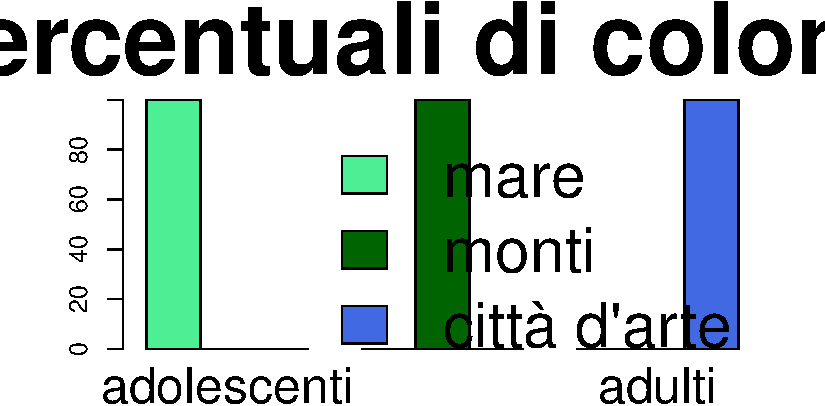
\includegraphics[width=0.4\linewidth,height=\textheight,keepaspectratio]{dispensa-statistica-descrittiva_files/figure-pdf/unnamed-chunk-110-1.pdf}
\end{center}

\textbf{Frequenze osservate}

\begin{Shaded}
\begin{Highlighting}[]
\NormalTok{obs\_n }\OtherTok{\textless{}{-}} \FunctionTok{matrix}\NormalTok{(}
  \FunctionTok{c}\NormalTok{(}\DecValTok{84}\NormalTok{, }\DecValTok{0}\NormalTok{, }\DecValTok{0}\NormalTok{,    }\CommentTok{\# mare → solo adolescenti}
    \DecValTok{0}\NormalTok{, }\DecValTok{64}\NormalTok{, }\DecValTok{0}\NormalTok{,    }\CommentTok{\# monti → solo giovani}
    \DecValTok{0}\NormalTok{, }\DecValTok{0}\NormalTok{, }\DecValTok{20}\NormalTok{),  }\CommentTok{\# città d’arte → solo adulti}
  \AttributeTok{nrow =} \DecValTok{3}\NormalTok{, }\AttributeTok{byrow =} \ConstantTok{TRUE}\NormalTok{) ; obs\_n}
\end{Highlighting}
\end{Shaded}

\begin{verbatim}
     [,1] [,2] [,3]
[1,]   84    0    0
[2,]    0   64    0
[3,]    0    0   20
\end{verbatim}

\textbf{Frequenze teoriche}

\begin{Shaded}
\begin{Highlighting}[]
\FunctionTok{chisq.test}\NormalTok{(obs\_n)}\SpecialCharTok{$}\NormalTok{expected}
\end{Highlighting}
\end{Shaded}

\begin{verbatim}
     [,1]      [,2]      [,3]
[1,]   42 32.000000 10.000000
[2,]   32 24.380952  7.619048
[3,]   10  7.619048  2.380952
\end{verbatim}

\begin{longtable}[]{@{}rrr@{}}
\caption{Frequenze osservate}\tabularnewline
\toprule\noalign{}
\endfirsthead
\endhead
\bottomrule\noalign{}
\endlastfoot
84 & 0 & 0 \\
0 & 64 & 0 \\
0 & 0 & 20 \\
\end{longtable}

\begin{longtable}[]{@{}rrr@{}}
\caption{Frequenze Teoriche}\tabularnewline
\toprule\noalign{}
\endfirsthead
\endhead
\bottomrule\noalign{}
\endlastfoot
42 & 32.000000 & 10.000000 \\
32 & 24.380952 & 7.619048 \\
10 & 7.619048 & 2.380952 \\
\end{longtable}

\begin{Shaded}
\begin{Highlighting}[]
\FunctionTok{chisq.test}\NormalTok{(obs\_n)}\SpecialCharTok{$}\NormalTok{statistic}
\end{Highlighting}
\end{Shaded}

\begin{verbatim}
Warning in chisq.test(obs_n): L'approssimazione al Chi-quadrato potrebbe essere
inesatta
\end{verbatim}

\begin{verbatim}
X-squared 
      336 
\end{verbatim}

\begin{Shaded}
\begin{Highlighting}[]
\FunctionTok{sum}\NormalTok{(obs\_n) }\SpecialCharTok{*} \FunctionTok{min}\NormalTok{(}\FunctionTok{c}\NormalTok{(}\FunctionTok{nrow}\NormalTok{(obs\_n) }\SpecialCharTok{{-}}\DecValTok{1}\NormalTok{, }
                            \FunctionTok{ncol}\NormalTok{(obs\_n) }\SpecialCharTok{{-}} \DecValTok{1}\NormalTok{))}
\end{Highlighting}
\end{Shaded}

\begin{verbatim}
[1] 336
\end{verbatim}

\section{Associazione (variabili
quantitative)}\label{associazione-variabili-quantitative}

\subsection{Relazione lineare}\label{relazione-lineare}

Si vuole studiare la \textbf{relazione lineare} tra due variabili
quantitative \(X\) e \(Y\) misurate sulle stesse unità statistiche

Per relazione lineare si intende quanto le coppie di punti
\((x_i, y_i)\) tendono a disporsi lungo una retta

\begin{center}
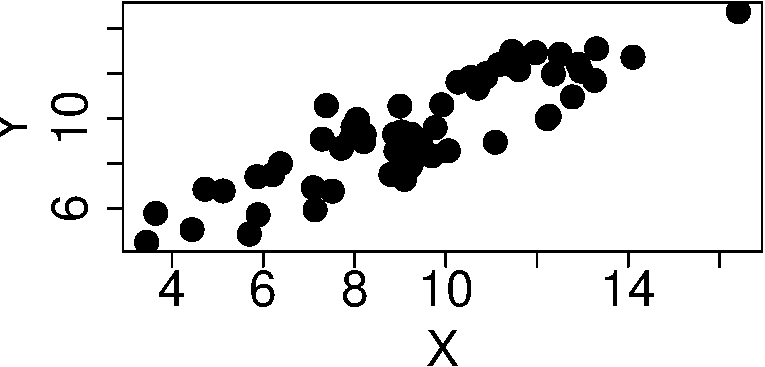
\includegraphics[width=0.45\linewidth,height=\textheight,keepaspectratio]{dispensa-statistica-descrittiva_files/figure-pdf/unnamed-chunk-115-1.pdf}
\end{center}

Due indici: la \textbf{covarianza} (direzione della relazione) e il
\textbf{coefficiente di correlazione lineare di Bravais-Pearson}
(direzione e intensità)

\subsection{Indice di covarianza
campionaria}\label{indice-di-covarianza-campionaria}

\begin{figure}[H]

{\centering 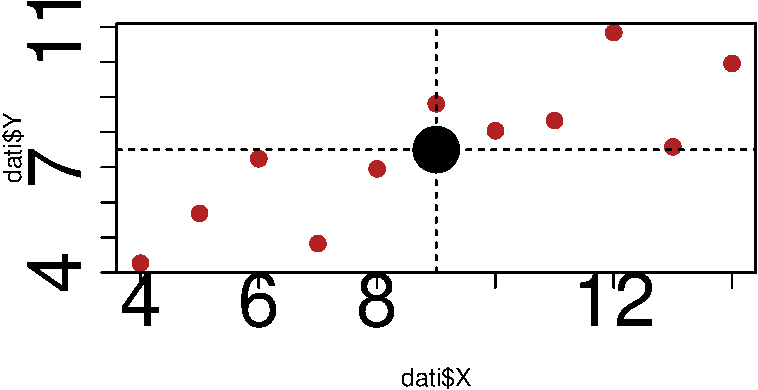
\includegraphics[width=0.7\linewidth,height=\textheight,keepaspectratio]{dispensa-statistica-descrittiva_files/figure-pdf/unnamed-chunk-117-1.pdf}

}

\caption{Grafico a dispersione delle variabili X e Y}

\end{figure}%

\begin{verbatim}
    X     Y
1  10  8.04
2   8  6.95
3  13  7.58
4   9  8.81
5  11  8.33
6  14  9.96
7   6  7.24
8   4  4.26
9  12 10.84
10  7  4.82
11  5  5.68
\end{verbatim}

\texttt{plot(x,\ y)}: Grafico di dispersione di due variabili
quantitative appaiate \texttt{(x,y)} aventi lo stesso numero di
osservazioni

\begin{Shaded}
\begin{Highlighting}[]
\NormalTok{X }\OtherTok{\textless{}{-}} \FunctionTok{c}\NormalTok{(}\DecValTok{9}\NormalTok{,}\DecValTok{8}\NormalTok{,}\DecValTok{12}\NormalTok{,}\DecValTok{9}\NormalTok{,}\DecValTok{10}\NormalTok{,}\DecValTok{14}\NormalTok{,}\DecValTok{5}\NormalTok{,}\DecValTok{4}\NormalTok{,}\DecValTok{13}\NormalTok{,}\DecValTok{7}\NormalTok{,}\DecValTok{5}\NormalTok{)}
\NormalTok{Y }\OtherTok{\textless{}{-}} \FunctionTok{c}\NormalTok{(}\DecValTok{9}\NormalTok{,}\DecValTok{6}\NormalTok{,}\DecValTok{8}\NormalTok{,}\DecValTok{9}\NormalTok{,}\DecValTok{7}\NormalTok{,}\DecValTok{10}\NormalTok{,}\DecValTok{8}\NormalTok{,}\DecValTok{4}\NormalTok{,}\DecValTok{11}\NormalTok{,}\DecValTok{5}\NormalTok{,}\DecValTok{4}\NormalTok{)}
\FunctionTok{plot}\NormalTok{(X,Y,}\AttributeTok{main=}\StringTok{"Grafico di dispersione"}\NormalTok{, }\AttributeTok{xlim=}\FunctionTok{c}\NormalTok{(}\DecValTok{0}\NormalTok{,}\DecValTok{20}\NormalTok{),}\AttributeTok{ylim=}\FunctionTok{c}\NormalTok{(}\DecValTok{0}\NormalTok{,}\DecValTok{15}\NormalTok{))}
\end{Highlighting}
\end{Shaded}

\begin{center}
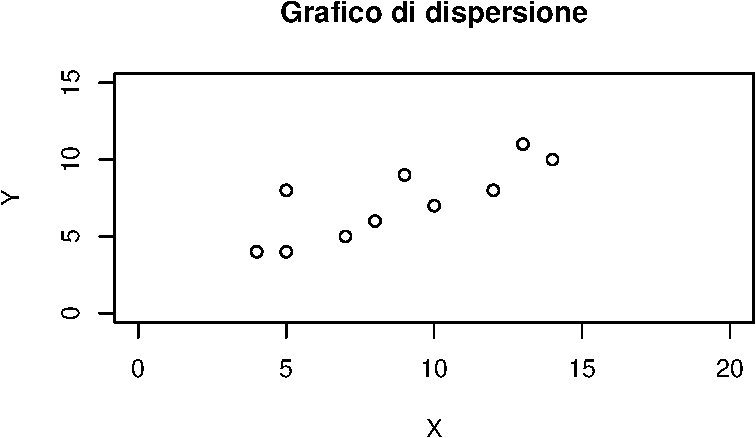
\includegraphics[width=0.6\linewidth,height=\textheight,keepaspectratio]{dispensa-statistica-descrittiva_files/figure-pdf/unnamed-chunk-119-1.pdf}
\end{center}

La \textbf{Covarianza} misura il grado di \emph{dispersione} e
\emph{covariazione} di due variabili quantitative appaiate \((X,Y)\)
attorno ai loro baricentri (medie) \(\bar{X}\) e \(\bar{Y}\)

\(x = (x_1, x_2, \ldots, x_n)\)

\(y = (y_1, y_2, \ldots, y_n)\)

\[d = ((x_1, y_1), (x_2, y_2), \ldots, (x_n, y_n))\]

\[\cov(x,y) = \dfrac{1}{n-1}\sum_{i=1}^n(x_i-\bar{x})(y_i
-\bar{y})\]

È (quasi) la \textbf{media dei prodotti degli scarti} di ogni variabile
dalla propria media

\begin{tcolorbox}[enhanced jigsaw, toprule=.15mm, left=2mm, leftrule=.75mm, breakable, coltitle=black, title={Note}, bottomtitle=1mm, opacitybacktitle=0.6, toptitle=1mm, titlerule=0mm, bottomrule=.15mm, colframe=quarto-callout-note-color-frame, arc=.35mm, rightrule=.15mm, opacityback=0, colbacktitle=quarto-callout-note-color!10!white, colback=white]

Nota: alcuni testi dividono per \(n\) invece che per \(n-1\) (covarianza
``descrittiva''). La funzione \texttt{cov()} di \texttt{R} divide per
\(n-1\), quindi useremo sempre questa versione

\end{tcolorbox}

\(\cov(X,Y) > 0\)

\begin{center}
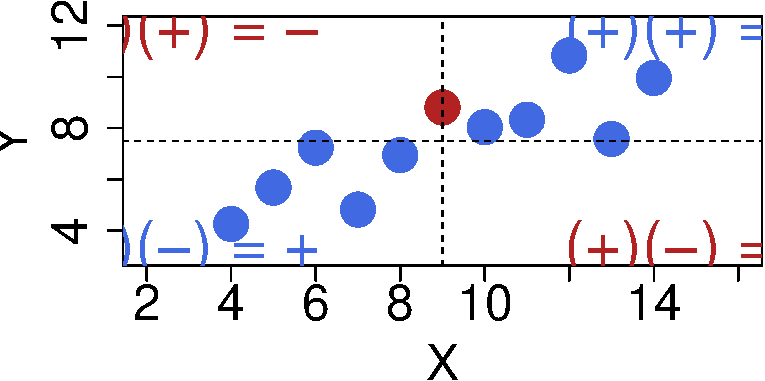
\includegraphics[width=1\linewidth,height=\textheight,keepaspectratio]{dispensa-statistica-descrittiva_files/figure-pdf/unnamed-chunk-120-1.pdf}
\end{center}

\(\cov(X,Y) < 0\)

\begin{center}
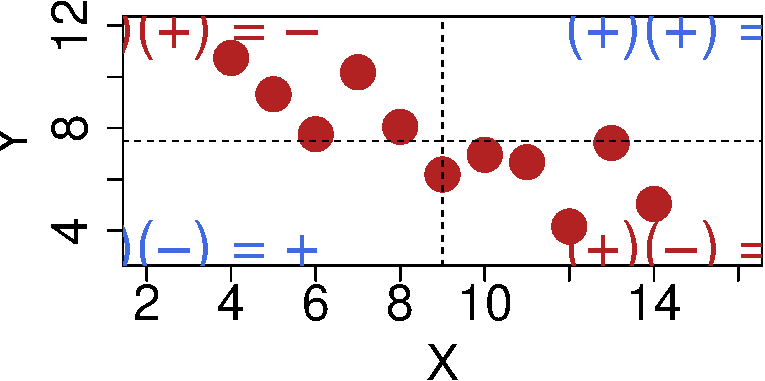
\includegraphics[width=1\linewidth,height=\textheight,keepaspectratio]{dispensa-statistica-descrittiva_files/figure-pdf/unnamed-chunk-121-1.pdf}
\end{center}

Il prodotto \((x_i - \bar{x})(y_i - \bar{y})\) è più spesso positivo se
\(\cov > 0\), più spesso negativo se \(\cov < 0\)

\begin{itemize}
\tightlist
\item
  La covarianza può assumere \textbf{tutti i valori reali}
\end{itemize}

\vspace{3mm}

\begin{itemize}
\tightlist
\item
  \(\cov(X,Y) > 0\): tendenza alla linearità positiva
  (\textbf{crescente})
\end{itemize}

\vspace{3mm}

\begin{itemize}
\tightlist
\item
  \(\cov(X,Y) < 0\): tendenza alla linearità negativa
  (\textbf{decrescente})
\end{itemize}

\vspace{3mm}

\begin{itemize}
\tightlist
\item
  \(\cov(X,Y) \approx 0\): nessuna tendenza lineare
\end{itemize}

Il valore della covarianza dipende dall'unità di misura delle variabili
\(\rightarrow\) ci dice la \textbf{direzione} della relazione ma non la
sua \textbf{intensità}

\begin{figure}

\begin{minipage}{0.50\linewidth}

\begin{figure}[H]

{\centering 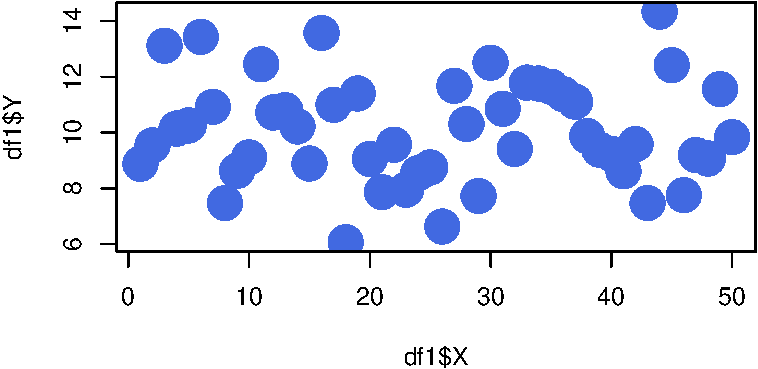
\includegraphics[width=0.6\linewidth,height=\textheight,keepaspectratio]{dispensa-statistica-descrittiva_files/figure-pdf/unnamed-chunk-123-1.pdf}

}

\subcaption{Cov = 0}

\end{figure}%

\end{minipage}%
%
\begin{minipage}{0.50\linewidth}

\begin{figure}[H]

{\centering 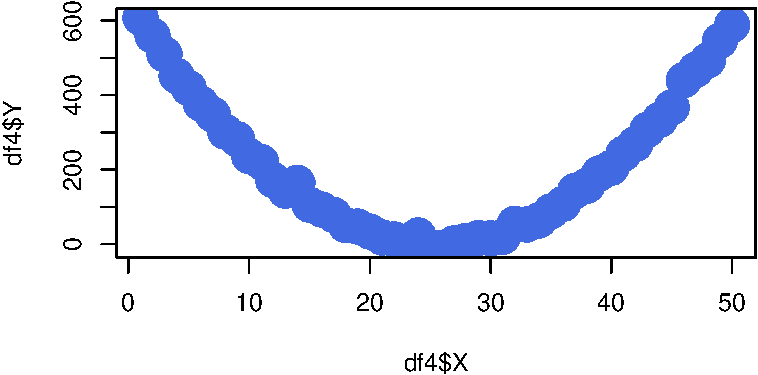
\includegraphics[width=0.6\linewidth,height=\textheight,keepaspectratio]{dispensa-statistica-descrittiva_files/figure-pdf/unnamed-chunk-123-2.pdf}

}

\subcaption{Cov = 0}

\end{figure}%

\end{minipage}%
\newline
\begin{minipage}{0.50\linewidth}

\begin{figure}[H]

{\centering 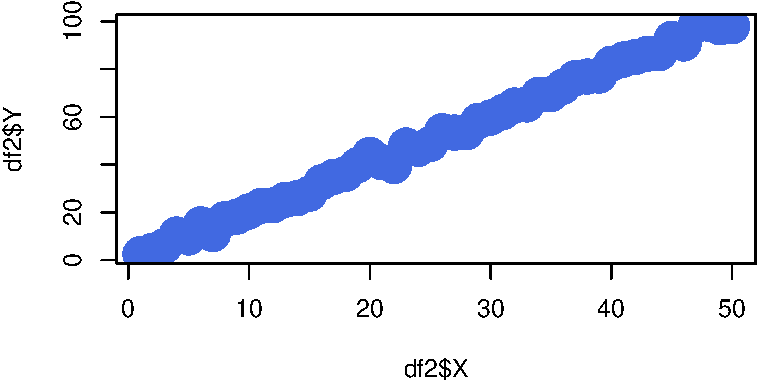
\includegraphics[width=0.6\linewidth,height=\textheight,keepaspectratio]{dispensa-statistica-descrittiva_files/figure-pdf/unnamed-chunk-123-3.pdf}

}

\subcaption{Cov \textgreater{} 0}

\end{figure}%

\end{minipage}%
%
\begin{minipage}{0.50\linewidth}

\begin{figure}[H]

{\centering 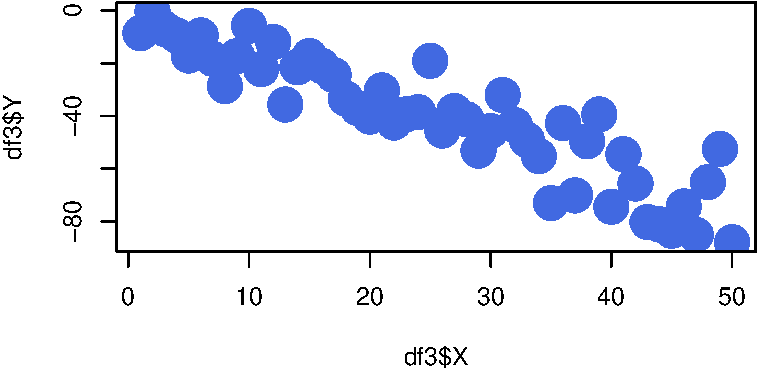
\includegraphics[width=0.6\linewidth,height=\textheight,keepaspectratio]{dispensa-statistica-descrittiva_files/figure-pdf/unnamed-chunk-123-4.pdf}

}

\subcaption{Cov \textless{} 0}

\end{figure}%

\end{minipage}%
\newline
\begin{minipage}{0.50\linewidth}
Covarianza\end{minipage}%

\end{figure}%

Età (in mesi) e peso (in kg) di un bambino rilevati in 6 momenti

\begin{verbatim}
  eta peso
1   3    6
2   6    8
3   9    9
4  12   10
5  24   13
6  36   20
\end{verbatim}

\begin{figure}[H]

{\centering 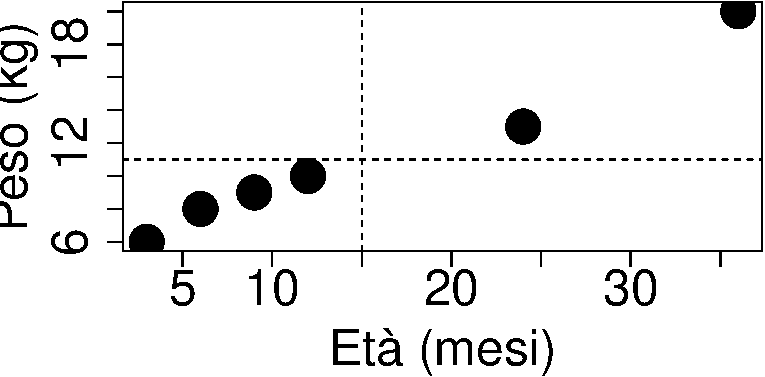
\includegraphics[width=0.7\linewidth,height=\textheight,keepaspectratio]{dispensa-statistica-descrittiva_files/figure-pdf/unnamed-chunk-126-1.pdf}

}

\caption{Grafico a dispersione}

\end{figure}%

\subsubsection{Calcolo della covarianza}\label{calcolo-della-covarianza}

\begin{verbatim}
   x  y x - media(x) y - media(y) prodotto
1  3  6          -12           -5       60
2  6  8           -9           -3       27
3  9  9           -6           -2       12
4 12 10           -3           -1        3
5 24 13            9            2       18
6 36 20           21            9      189
\end{verbatim}

\(\bar{x} = 15\), \(\bar{y} = 11\),
\(\sum_i (x_i - \bar{x})(y_i - \bar{y}) = 309\)

\[\cov(x,y) = \dfrac{309}{6-1} = 61.8\]

E quindi? Sappiamo che la relazione è \textbf{positiva}, ma è forte o
debole?

\subsection{\texorpdfstring{\texttt{cov()}}{cov()}}\label{cov}

\texttt{cov()}: Restituisce la covarianza campionaria tra due variabili
quantitative appaiate \((X,Y)\) aventi lo stesso numero di osservazioni

\begin{Shaded}
\begin{Highlighting}[]
\NormalTok{X }\OtherTok{\textless{}{-}} \FunctionTok{c}\NormalTok{(}\DecValTok{9}\NormalTok{,}\DecValTok{8}\NormalTok{,}\DecValTok{12}\NormalTok{,}\DecValTok{9}\NormalTok{,}\DecValTok{10}\NormalTok{,}\DecValTok{14}\NormalTok{,}\DecValTok{5}\NormalTok{,}\DecValTok{4}\NormalTok{,}\DecValTok{13}\NormalTok{,}\DecValTok{7}\NormalTok{,}\DecValTok{5}\NormalTok{)}
\NormalTok{Y }\OtherTok{\textless{}{-}} \FunctionTok{c}\NormalTok{(}\DecValTok{9}\NormalTok{,}\DecValTok{6}\NormalTok{,}\DecValTok{8}\NormalTok{,}\DecValTok{9}\NormalTok{,}\DecValTok{7}\NormalTok{,}\DecValTok{10}\NormalTok{,}\DecValTok{8}\NormalTok{,}\DecValTok{4}\NormalTok{,}\DecValTok{11}\NormalTok{,}\DecValTok{5}\NormalTok{,}\DecValTok{4}\NormalTok{)}
\NormalTok{Z }\OtherTok{\textless{}{-}} \SpecialCharTok{{-}}\NormalTok{Y}
\FunctionTok{cov}\NormalTok{(X,Y)}
\end{Highlighting}
\end{Shaded}

\begin{verbatim}
[1] 6.309091
\end{verbatim}

\begin{Shaded}
\begin{Highlighting}[]
\FunctionTok{cov}\NormalTok{(X,Z)}
\end{Highlighting}
\end{Shaded}

\begin{verbatim}
[1] -6.309091
\end{verbatim}

\begin{Shaded}
\begin{Highlighting}[]
\FunctionTok{cov}\NormalTok{(bimbo}\SpecialCharTok{$}\NormalTok{eta, bimbo}\SpecialCharTok{$}\NormalTok{peso)}
\end{Highlighting}
\end{Shaded}

\begin{verbatim}
[1] 61.8
\end{verbatim}

\subsection{Correlazione campionaria}\label{correlazione-campionaria}

Per stabilire l'\textbf{intensità} della relazione la covarianza va
\emph{normalizzata}, ovvero divisa per il suo valore massimo

\vspace{2mm}

\(-sd(x)sd(y) \leq\cov(X,Y)\leq + sd(x)sd(y)\)

\[r  = \dfrac{\cov(X,Y)}{sd(x)sd(y)}\]

\[-1 \leq r \leq 1\] \(r = +1\): legame \textbf{perfettamente lineare e
diretto};

\(r = -1\): legame \textbf{perfettamente lineare e inverso}

\(r = 0\): \textbf{incorrelazione}: non esiste un legame
\emph{lineare}\ldots{} ma questo non implica che le variabili non siano
in relazione tra loro

\begin{center}
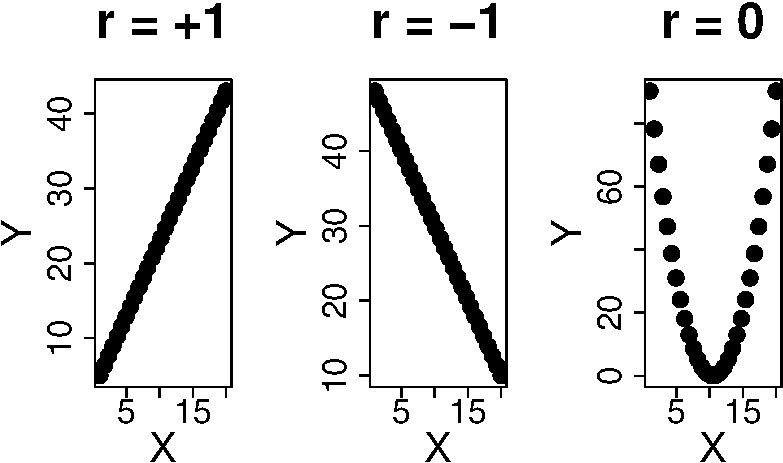
\includegraphics[width=1\linewidth,height=\textheight,keepaspectratio]{dispensa-statistica-descrittiva_files/figure-pdf/unnamed-chunk-129-1.pdf}
\end{center}

\subsection{\texorpdfstring{\texttt{cor()}}{cor()}}\label{cor}

\texttt{cor()}: Restituisce la correlazione (lineare) campionaria tra
due variabili quantitative appaiate \((X,Y)\) aventi lo stesso numero di
osservazioni

\begin{Shaded}
\begin{Highlighting}[]
\NormalTok{X }\OtherTok{\textless{}{-}} \FunctionTok{c}\NormalTok{(}\DecValTok{9}\NormalTok{,}\DecValTok{8}\NormalTok{,}\DecValTok{12}\NormalTok{,}\DecValTok{9}\NormalTok{,}\DecValTok{10}\NormalTok{,}\DecValTok{14}\NormalTok{,}\DecValTok{5}\NormalTok{,}\DecValTok{4}\NormalTok{,}\DecValTok{13}\NormalTok{,}\DecValTok{7}\NormalTok{,}\DecValTok{5}\NormalTok{)}
\NormalTok{Y }\OtherTok{\textless{}{-}} \FunctionTok{c}\NormalTok{(}\DecValTok{9}\NormalTok{,}\DecValTok{6}\NormalTok{,}\DecValTok{8}\NormalTok{,}\DecValTok{9}\NormalTok{,}\DecValTok{7}\NormalTok{,}\DecValTok{10}\NormalTok{,}\DecValTok{8}\NormalTok{,}\DecValTok{4}\NormalTok{,}\DecValTok{11}\NormalTok{,}\DecValTok{5}\NormalTok{,}\DecValTok{4}\NormalTok{)}
\NormalTok{Z }\OtherTok{\textless{}{-}} \SpecialCharTok{{-}}\NormalTok{Y}
\FunctionTok{cor}\NormalTok{(X,Y)}
\end{Highlighting}
\end{Shaded}

\begin{verbatim}
[1] 0.7921487
\end{verbatim}

\begin{Shaded}
\begin{Highlighting}[]
\FunctionTok{cor}\NormalTok{(X,Z)}
\end{Highlighting}
\end{Shaded}

\begin{verbatim}
[1] -0.7921487
\end{verbatim}

\subsubsection{Il bambino di prima}\label{il-bambino-di-prima}

\begin{Shaded}
\begin{Highlighting}[]
\FunctionTok{cov}\NormalTok{(bimbo}\SpecialCharTok{$}\NormalTok{eta, bimbo}\SpecialCharTok{$}\NormalTok{peso) }\SpecialCharTok{/}\NormalTok{ (}\FunctionTok{sd}\NormalTok{(bimbo}\SpecialCharTok{$}\NormalTok{eta) }\SpecialCharTok{*} \FunctionTok{sd}\NormalTok{(bimbo}\SpecialCharTok{$}\NormalTok{peso))}
\end{Highlighting}
\end{Shaded}

\begin{verbatim}
[1] 0.9860185
\end{verbatim}

\begin{Shaded}
\begin{Highlighting}[]
\FunctionTok{cor}\NormalTok{(bimbo}\SpecialCharTok{$}\NormalTok{eta, bimbo}\SpecialCharTok{$}\NormalTok{peso)}
\end{Highlighting}
\end{Shaded}

\begin{verbatim}
[1] 0.9860185
\end{verbatim}

\[r = \dfrac{61.8}{12.59 \cdot 4.98} = 0.986\]

Le variabili presentano una \textbf{fortissima correlazione positiva}: i
punti tendono a disporsi lungo una retta crescente

\begin{center}
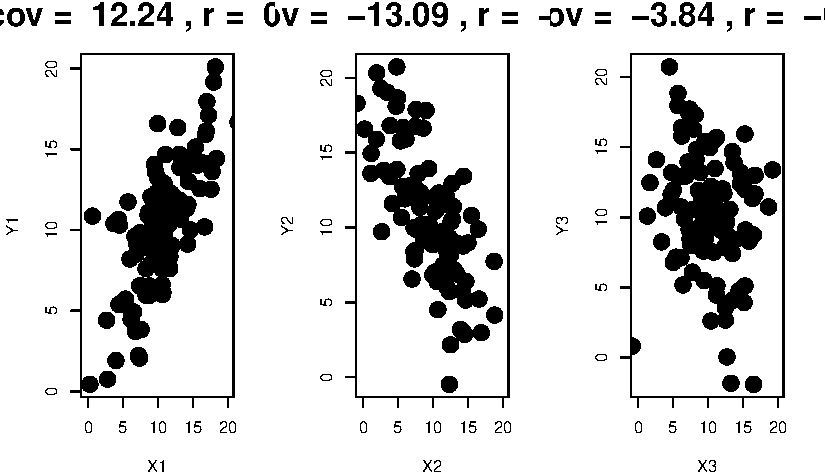
\includegraphics[width=0.7\linewidth,height=\textheight,keepaspectratio]{dispensa-statistica-descrittiva_files/figure-pdf/unnamed-chunk-132-1.pdf}
\end{center}

\begin{center}

\includegraphics[width=0.7\linewidth,height=\textheight,keepaspectratio]{slides/modulo3/cor2.jpg}
\end{center}

\subsection{\texorpdfstring{Usi e abusi di
\(r\)}{Usi e abusi di r}}\label{usi-e-abusi-di-r}

\subsubsection{\texorpdfstring{In
\(\psi\)}{In \textbackslash psi}}\label{in-psi}

\begin{itemize}
\item
  Attendibilità test-retest
\item
  Forme parallele di un test (coefficiente di equivalenza)
\item
  Accordo tra le valutazioni di due giudici
\item
  Consistenza interna di un questionario
\item
  \ldots{}
\end{itemize}

\subsubsection{Statistics doesn't lie, but liars use
statistics}\label{statistics-doesnt-lie-but-liars-use-statistics}

Due variabili possono essere fortemente correlate senza che esista alcun
legame tra di loro

\vspace{3mm}

\begin{center}
\url{https://www.tylervigen.com/spurious-correlations}
\end{center}

\vspace{3mm}

\begin{center}
\textbf{Correlazione $\neq$ causalità}
\end{center}

\vspace{2mm}

\begin{center}
\textit{L'ignoranza afferma o nega rotondamente; la scienza dubita} (Voltaire)
\end{center}

\subsubsection{Relazione diretta}\label{relazione-diretta}

\begin{center}
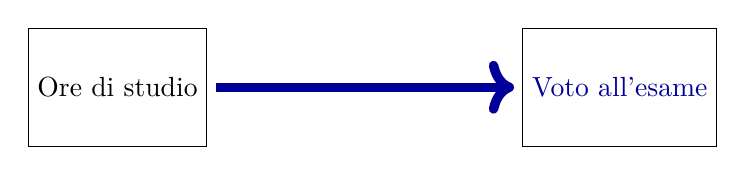
\begin{tikzpicture}[
  squarednode/.style={rectangle, draw=black, minimum size=15mm, align=center},
  ]
  \node[squarednode] (x) {Ore di studio};
  \node[squarednode] (y) [right=4cm of x] {\textcolor{blue!60!black}{Voto all'esame}};
  \draw[->, line width=0.12cm, shorten >= +3pt, shorten <= +3pt, blue!60!black] (x.east) -- (y.west);
\end{tikzpicture}
\end{center}

\vspace{5mm}

Ma ne siamo proprio sicuri?

\subsubsection{Relazione indiretta}\label{relazione-indiretta}

\begin{center}
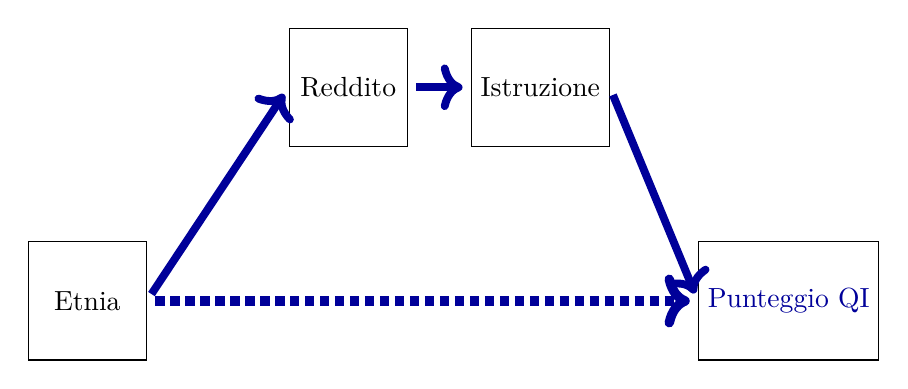
\begin{tikzpicture}[
  squarednode/.style={rectangle, draw=black, minimum size=15mm, align=center},
  ]
  \node[squarednode] (x) {Etnia};
  \node[squarednode] (y) [right=7cm of x] {\textcolor{blue!60!black}{Punteggio QI}};
  \node[squarednode] (z1) [above right=1.2cm and 1.8cm of x] {Reddito};
  \node[squarednode] (z2) [right=0.8cm of z1] {Istruzione};
  \draw[dotted, ->, line width=0.12cm, shorten >= +3pt, shorten <= +3pt, blue!60!black] (x.east) -- (y.west);
  \draw[->, line width=0.10cm, shorten >= +3pt, shorten <= +3pt, blue!60!black] (x.east) -- (z1.west);
  \draw[->, line width=0.10cm, shorten >= +3pt, shorten <= +3pt, blue!60!black] (z1.east) -- (z2.west);
  \draw[->, line width=0.10cm, shorten >= +3pt, shorten <= +3pt, blue!60!black] (z2.east) -- (y.west);
\end{tikzpicture}
\end{center}

La relazione tra \(X\) e \(Y\) passa attraverso altre variabili
(mediatori)

\subsubsection{Relazione spuria}\label{relazione-spuria}

\begin{center}
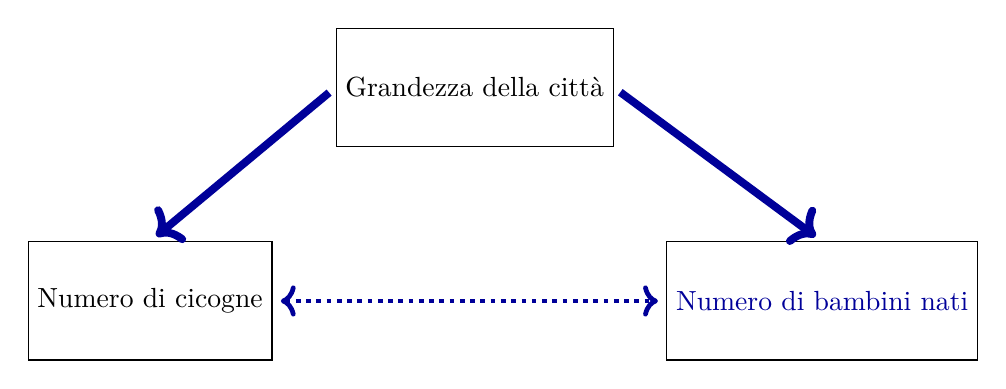
\begin{tikzpicture}[
  squarednode/.style={rectangle, draw=black, minimum size=15mm, align=center},
  ]
  \node[squarednode] (x) {Numero di cicogne};
  \node[squarednode] (y) [right=5cm of x] {\textcolor{blue!60!black}{Numero di bambini nati}};
  \node[squarednode] (z) [above right=1.2cm and 0.8cm of x] {Grandezza della città};
  \draw[dotted, <->, line width=0.06cm, shorten >= +3pt, shorten <= +3pt, blue!60!black] (x.east) -- (y.west);
  \draw[->, line width=0.10cm, shorten >= +3pt, shorten <= +3pt, blue!60!black] (z.west) -- (x.north);
  \draw[->, line width=0.10cm, shorten >= +3pt, shorten <= +3pt, blue!60!black] (z.east) -- (y.north);
\end{tikzpicture}
\end{center}

\(X\) e \(Y\) sono correlate solo perché entrambe dipendono da una terza
variabile

\vspace{3mm}

\begin{center}
\normalsize LA STATISTICA SOSTIENE, NON ILLUMINA!
\end{center}

\section{Previsione variabili
quantitative}\label{previsione-variabili-quantitative}

\subsection{Regressione lineare}\label{regressione-lineare}

\subsubsection{\texorpdfstring{Quanto varia \(y\) in funzione di
\(x\)?}{Quanto varia y in funzione di x?}}\label{quanto-varia-y-in-funzione-di-x}

La correlazione permette di stabilire quanto covariano due variabili,
\(x\) e \(y\): \textbf{modello simmetrico} per determinare
\emph{l'intensità della relazione}

Con un modello di regressione si vuole andare più a fondo per capire
\textbf{quanto} varia \(y\) in funzione di ogni cambiamento in \(x\):
stabilire non solo se le variabili sono associate o meno ma la portata
della variazione

La relazione è \emph{asimettrica}: si vuole spiegare \(y\) in funzione
di \(x\) (questo non vuol dire in alcun modo che la relazione sia
causale)

\begin{center}
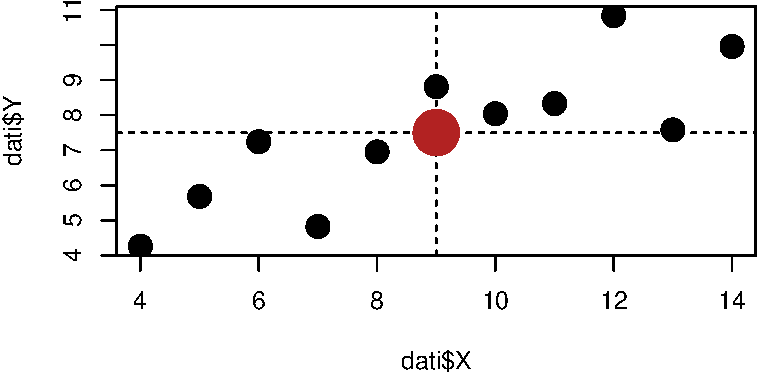
\includegraphics[width=0.7\linewidth,height=\textheight,keepaspectratio]{dispensa-statistica-descrittiva_files/figure-pdf/unnamed-chunk-134-1.pdf}
\end{center}

\begin{verbatim}
    X     Y
1  10  8.04
2   8  6.95
3  13  7.58
4   9  8.81
5  11  8.33
6  14  9.96
7   6  7.24
8   4  4.26
9  12 10.84
10  7  4.82
11  5  5.68
\end{verbatim}

\[r = 0.79\]

\begin{figure}[H]

{\centering 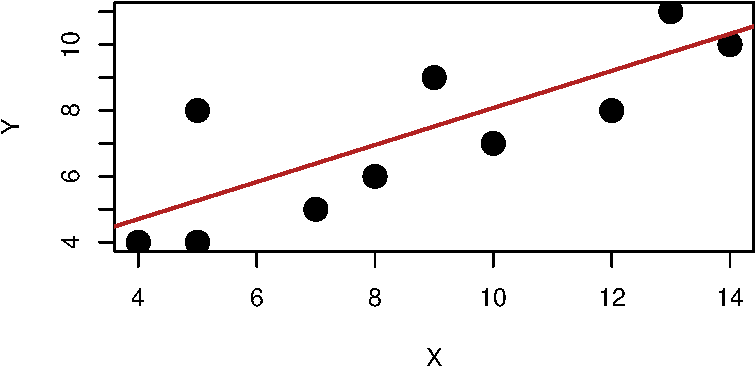
\includegraphics[width=0.7\linewidth,height=\textheight,keepaspectratio]{dispensa-statistica-descrittiva_files/figure-pdf/unnamed-chunk-136-1.pdf}

}

\caption{Una retta che passi attraverso le coppie di osservazioni}

\end{figure}%

\begin{figure}[H]

{\centering 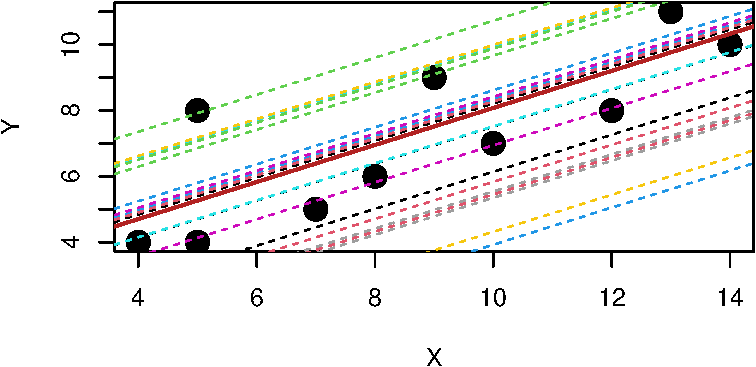
\includegraphics[width=0.7\linewidth,height=\textheight,keepaspectratio]{dispensa-statistica-descrittiva_files/figure-pdf/unnamed-chunk-137-1.pdf}

}

\caption{Ma quale retta?}

\end{figure}%

Caso estremamente semplice dove varia solo l'intercetta -- le rette sono
parallele

La regressione lineare tra una \emph{variabile indipendente} \(X\)
(predittore) ed una \emph{variabile dipendente} \(Y\) (criterio) calcola
la migliore approssimazione lineare che identifica il legame tra le due
variabili utilizzando la struttura di dati bivariata \((x_i,y_i)\)
osservata su un campione di \(n\) osservazioni.

\(x = (x_1, x_2, \ldots, x_n)\)

\(y = (y_1, y_2, \ldots, y_n)\)

\[d = ((x_1, y_1), (x_2, y_2), \ldots, (x_n, y_n))\]

\[Y = \beta_0 + \beta X \]
\[y_i = \beta_0 + \beta x_i + \varepsilon_i \quad (i = 1, \ldots, n)\]

\(y_i\): Valore di \(y\) atteso per l'i-esima osservazione

\(\beta_0\): Valore dell'intercetta, ovvero \emph{valore atteso in \(y\)
quando \(x_i = 0\)}

\(\beta_1\): Coefficiente angolare ovvero la pendenza della retta.
Definisce \emph{il cambiamento medio atteso in y per ogni cambiamento
unitario in \(x\)}

\(\varepsilon_i\): Componente d'errore (\(\mathcal{N}(0, \sigma^2)\))

\subsection{Principio dei minimi
quadrati}\label{principio-dei-minimi-quadrati}

\[SQE = \sum_{i=1}^n (y_i - y_i^*)^2 = \sum_{i=1}^n \bigl(y_i - (\beta_0 + \beta x_i)\bigr)^2  = \sum_{i=1}^n e_i^2\]

dove \(y_i^* = \beta_0 + \beta x_i\), e \(e_i = y_i - y_i^*\).
\normalsize

Per il principio dei minimi quadrati si può dimostrare che lo stimatore
ottimale per \(\beta\) è

\[\hat{\beta} = \frac{\operatorname{Cov}(X,Y)}{\operatorname{Var}(X)}
= \frac{\sum_{i=1}^n (x_i - \bar{x})(y_i - \bar{y})}{\sum_{i=1}^n (x_i - \bar{x})^2}\]

mentre per \(\beta_0\) è

\[\hat{\beta}_0 = \bar{y} - \hat{\beta}\,\bar{x}\]

\begin{center}
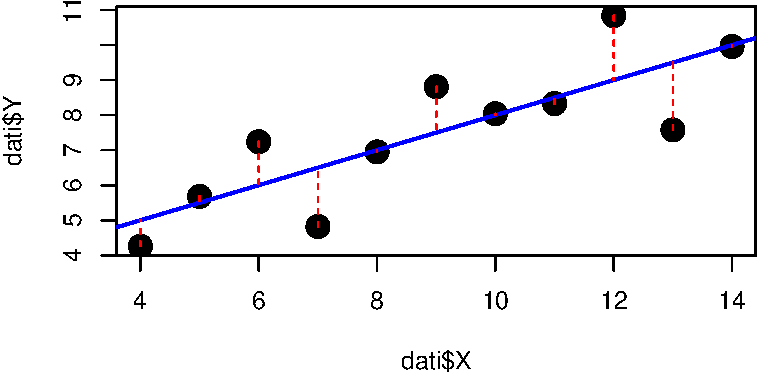
\includegraphics[width=0.7\linewidth,height=\textheight,keepaspectratio]{dispensa-statistica-descrittiva_files/figure-pdf/unnamed-chunk-138-1.pdf}
\end{center}

\subsection{Proprietà della retta di
regressione}\label{proprietuxe0-della-retta-di-regressione}

\subsubsection{Coefficiente angolare e
correlazione}\label{coefficiente-angolare-e-correlazione}

\[\hat{\beta} = \dfrac{\cov(X,Y)}{sd(x)^2}\]

\[r = \dfrac{\cov(X,Y)}{sd(x)sd(y)}\]

Moltiplicando e dividendo \(\hat{\beta}\) per \(sd(y)\):

\[\hat{\beta} = r \, \dfrac{sd(y)}{sd(x)}\]

\begin{enumerate}
\def\labelenumi{\arabic{enumi}.}
\item
  Il \textbf{segno} del coefficiente angolare è lo stesso di \(r\):
  \(r > 0 \Rightarrow\) retta crescente, \(r < 0 \Rightarrow\) retta
  decrescente, \(r = 0 \Rightarrow\) retta orizzontale
\item
  La retta passa sempre per il \textbf{punto delle medie}
  \((\bar{x}, \bar{y})\) (basta sostituire \(x = \bar{x}\) in
  \(\hat{y} = \hat{\beta}_0 + \hat{\beta}x\))
\end{enumerate}

\subsubsection{Il bambino di prima}\label{il-bambino-di-prima-1}

\begin{Shaded}
\begin{Highlighting}[]
\NormalTok{b }\OtherTok{\textless{}{-}} \FunctionTok{cov}\NormalTok{(bimbo}\SpecialCharTok{$}\NormalTok{eta, bimbo}\SpecialCharTok{$}\NormalTok{peso) }\SpecialCharTok{/} \FunctionTok{var}\NormalTok{(bimbo}\SpecialCharTok{$}\NormalTok{eta)}
\NormalTok{b0 }\OtherTok{\textless{}{-}} \FunctionTok{mean}\NormalTok{(bimbo}\SpecialCharTok{$}\NormalTok{peso) }\SpecialCharTok{{-}}\NormalTok{ b }\SpecialCharTok{*} \FunctionTok{mean}\NormalTok{(bimbo}\SpecialCharTok{$}\NormalTok{eta)}
\FunctionTok{c}\NormalTok{(b0, b)}
\end{Highlighting}
\end{Shaded}

\begin{verbatim}
[1] 5.1477273 0.3901515
\end{verbatim}

\begin{Shaded}
\begin{Highlighting}[]
\FunctionTok{cor}\NormalTok{(bimbo}\SpecialCharTok{$}\NormalTok{eta, bimbo}\SpecialCharTok{$}\NormalTok{peso) }\SpecialCharTok{*} \FunctionTok{sd}\NormalTok{(bimbo}\SpecialCharTok{$}\NormalTok{peso) }\SpecialCharTok{/} \FunctionTok{sd}\NormalTok{(bimbo}\SpecialCharTok{$}\NormalTok{eta)}
\end{Highlighting}
\end{Shaded}

\begin{verbatim}
[1] 0.3901515
\end{verbatim}

Retta di regressione: \(\hat{y} = 5.15 + 0.39x\)

Quale sarebbe il peso previsto a 48 mesi?
\(\hat{y}_{48} = 5.15 + 0.39 \cdot 48 = 23.88\) kg

\subsection{\texorpdfstring{Indice di adattamento
\(R^2\)}{Indice di adattamento R\^{}2}}\label{indice-di-adattamento-r2}

\[R^2 = 1 - \dfrac{SQE/n-1}{Var(Y)} = 1 - \dfrac{\sum_{i=1}^n e_i^2}{\sum_{i=1}^n (y_i - \bar{y})^2}\]

\(\varepsilon = \dfrac{SQE}{n-1}\): Stimatore campionario della varianza
della componente di errore

\(0\leq R^2 \leq 1\): Più \(R^2\) è vicino ad 1, migliore è il modello.
Di fatto, \(R^2 = r^2\)

\begin{center}
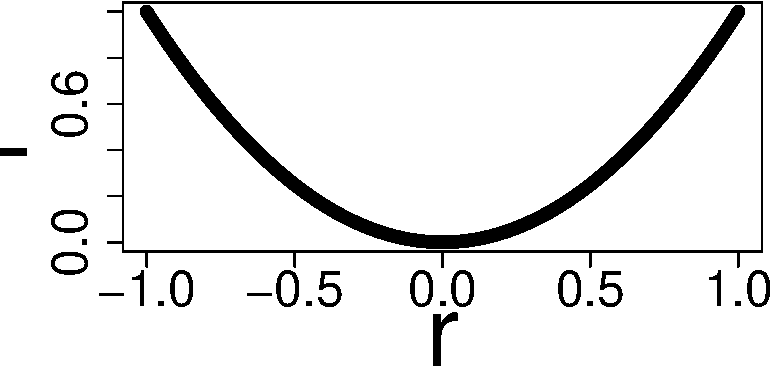
\includegraphics[width=0.7\linewidth,height=\textheight,keepaspectratio]{dispensa-statistica-descrittiva_files/figure-pdf/unnamed-chunk-140-1.pdf}
\end{center}

\begin{center}
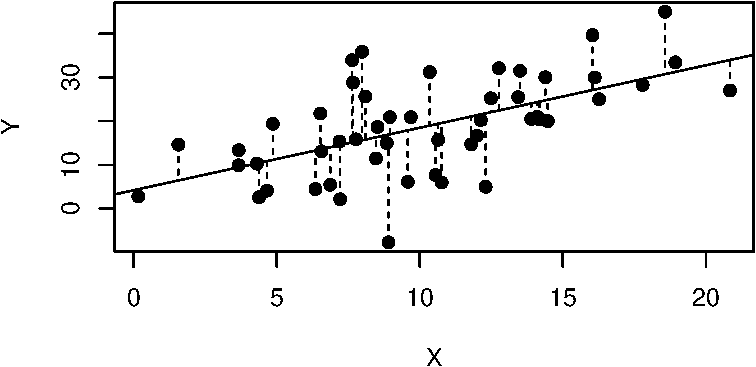
\includegraphics[width=0.8\linewidth,height=\textheight,keepaspectratio]{dispensa-statistica-descrittiva_files/figure-pdf/unnamed-chunk-141-1.pdf}
\end{center}

\(R^2 = 0.34\), \(r = 0.59\)

\begin{center}
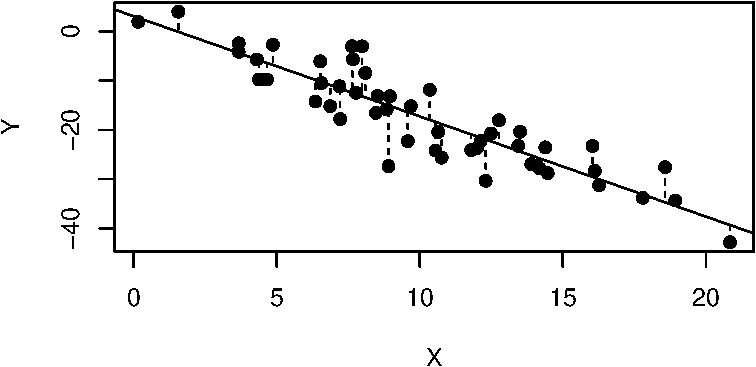
\includegraphics[width=0.8\linewidth,height=\textheight,keepaspectratio]{dispensa-statistica-descrittiva_files/figure-pdf/unnamed-chunk-142-1.pdf}
\end{center}

\(R^2 = 0.81\), \(r = -0.9\)

\begin{center}
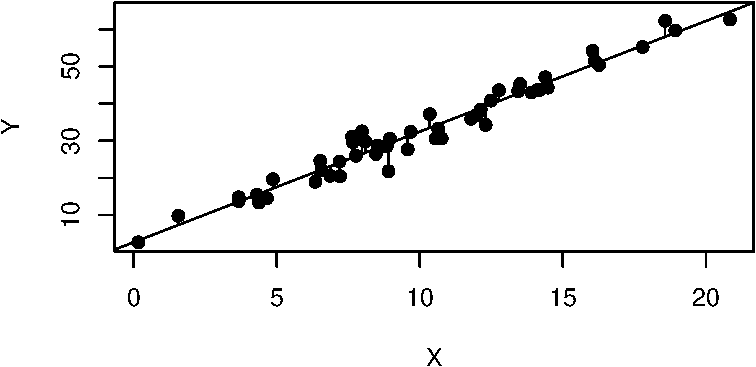
\includegraphics[width=0.8\linewidth,height=\textheight,keepaspectratio]{dispensa-statistica-descrittiva_files/figure-pdf/unnamed-chunk-143-1.pdf}
\end{center}

\(R^2 = 0.96\), \(r = 0.98\)

\begin{center}
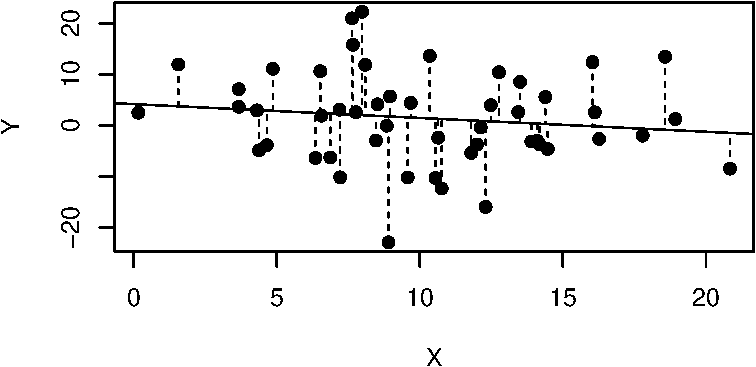
\includegraphics[width=0.8\linewidth,height=\textheight,keepaspectratio]{dispensa-statistica-descrittiva_files/figure-pdf/unnamed-chunk-144-1.pdf}
\end{center}

\(R^2 = 0\), \(r = -0.14\)

\subsection{\texorpdfstring{\texttt{lm()}}{lm()}}\label{lm}

\texttt{lm(Y\ \textasciitilde{}\ X)}: Retituisce la stima dei parametri
del modello di regressione lineare dove si predicono i valori di \(Y\) a
seconda dei valori di \(X\)

\texttt{\textasciitilde{}}: (Per i PC con tastierino numerico):
\texttt{ALT\ +\ 126}, Per i MAC: \texttt{ALT\ +\ 5} (fonte non
verificata)

\begin{Shaded}
\begin{Highlighting}[]
\NormalTok{X }\OtherTok{\textless{}{-}} \FunctionTok{c}\NormalTok{(}\DecValTok{9}\NormalTok{,}\DecValTok{8}\NormalTok{,}\DecValTok{12}\NormalTok{,}\DecValTok{9}\NormalTok{,}\DecValTok{10}\NormalTok{,}\DecValTok{14}\NormalTok{,}\DecValTok{5}\NormalTok{,}\DecValTok{4}\NormalTok{,}\DecValTok{13}\NormalTok{,}\DecValTok{7}\NormalTok{,}\DecValTok{5}\NormalTok{)}
\NormalTok{Y }\OtherTok{\textless{}{-}} \FunctionTok{c}\NormalTok{(}\DecValTok{9}\NormalTok{,}\DecValTok{6}\NormalTok{,}\DecValTok{8}\NormalTok{,}\DecValTok{9}\NormalTok{,}\DecValTok{7}\NormalTok{,}\DecValTok{10}\NormalTok{,}\DecValTok{8}\NormalTok{,}\DecValTok{4}\NormalTok{,}\DecValTok{11}\NormalTok{,}\DecValTok{5}\NormalTok{,}\DecValTok{4}\NormalTok{)}
\FunctionTok{lm}\NormalTok{(Y}\SpecialCharTok{\textasciitilde{}}\NormalTok{X)}
\end{Highlighting}
\end{Shaded}

\begin{verbatim}

Call:
lm(formula = Y ~ X)

Coefficients:
(Intercept)            X  
     2.4554       0.5624  
\end{verbatim}

\subsection{Assunti del modello}\label{assunti-del-modello}

\subsubsection{Assunzioni}\label{assunzioni}

\begin{itemize}
\tightlist
\item
  \textbf{Indipendenza dei predittori dall'errore}
\end{itemize}

\vspace{1.5mm}

\begin{quote}
I predittori sono misurati senza errore, ovvero i predittori e gli
errori di misura non sono correlati nella popolazione (per questo è
importante il campionamento casuale)
\end{quote}

\begin{itemize}
\tightlist
\item
  \textbf{Indipendenza delle osservazioni}
\end{itemize}

\vspace{1.5mm}

\begin{quote}
\(\forall i \neq j, \, \varepsilon_i \perp\!\!\!\perp \varepsilon_j\)
(le osservazioni sono state campionate indipendentemente l'una
dall'altra)
\end{quote}

\begin{itemize}
\tightlist
\item
  \textbf{Linearità}
\end{itemize}

\vspace{1.5mm}

\begin{quote}
Il valore atteso dell'errore per un dato valore di \(x\) è 0
\end{quote}

\subsubsection{Assunzioni}\label{assunzioni-1}

\begin{itemize}
\tightlist
\item
  \textbf{Normalità}
\end{itemize}

\vspace{1.5mm}

\begin{quote}
\(\varepsilon_i \sim \mathcal{N}(0, \sigma^2)\): Anche \(y_i\) è
distribuita normalmente con media \(\beta_0 + \beta_1x_i\)
\end{quote}

\begin{itemize}
\tightlist
\item
  \textbf{Varianza costante} (omoschedasticità)
\end{itemize}

\vspace{1.5mm}

\begin{quote}
La varianza degli errori è costante per qualunque valore di \(X\)
\end{quote}

\vspace{3mm}

Gli errori \(\varepsilon_i\) della popolazione non si osservano
\(\rightarrow\) si guardano i loro ``rappresentanti'' nel campione: i
\textbf{residui} \(e_i = y_i - \hat{y}_i\)

\textbf{Indipendenza dei predittori dall'errore}

\vspace{1.5mm}

\begin{quote}
I predittori sono misurati senza errore, ovvero i predittori e gli
errori di misura non sono correlati nella popolazione (per questo è
importante il campionamento casuale)
\end{quote}

\begin{center}
\emph{Analisi dei residui}
\end{center}

I residui e il predittore \textbf{non devono essere correlati tra di
loro}

\begin{center}
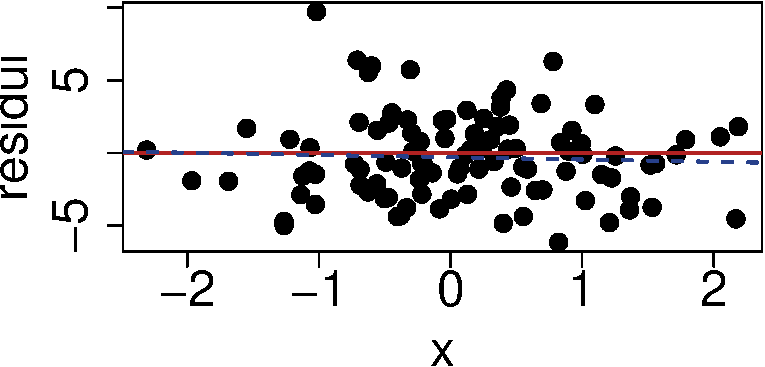
\includegraphics[width=0.7\linewidth,height=\textheight,keepaspectratio]{dispensa-statistica-descrittiva_files/figure-pdf/unnamed-chunk-146-1.pdf}
\end{center}

La linea intera rossa rappresenta quello che dovremmo osservare, ossia
la totale assenza di relazione tra la \(x\) e i residui del modello

Le linea tratteggiata blu indica la relazione effettiva tra i residui e
il predittore \(x\). Questa linea deve essere il più vicina possibile
alla linea rossa

\begin{center}
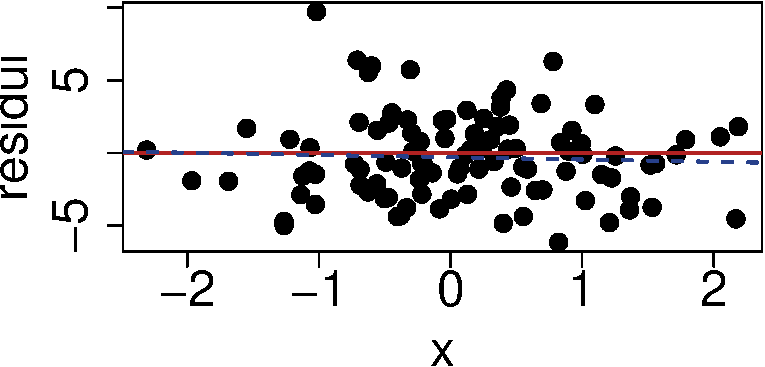
\includegraphics[width=0.7\linewidth,height=\textheight,keepaspectratio]{dispensa-statistica-descrittiva_files/figure-pdf/unnamed-chunk-147-1.pdf}
\end{center}

\[r = -0.05\]

\begin{center}
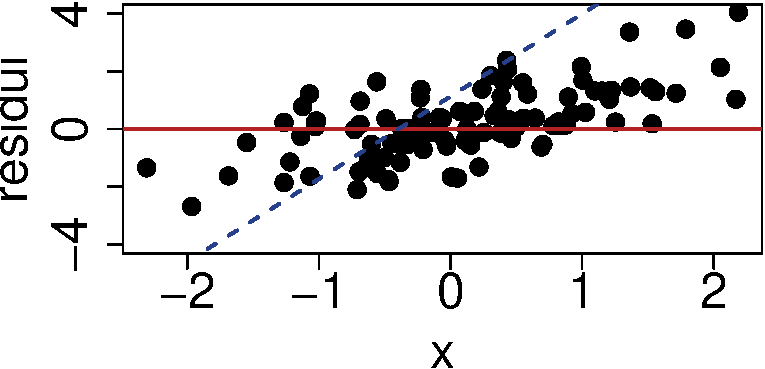
\includegraphics[width=0.7\linewidth,height=\textheight,keepaspectratio]{dispensa-statistica-descrittiva_files/figure-pdf/unnamed-chunk-148-1.pdf}
\end{center}

\begin{center}
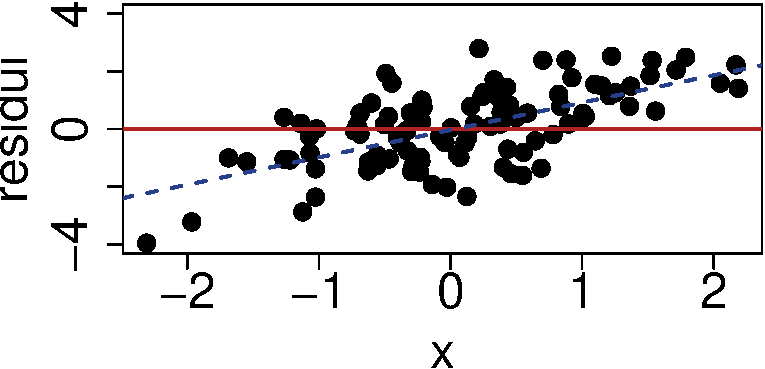
\includegraphics[width=0.7\linewidth,height=\textheight,keepaspectratio]{dispensa-statistica-descrittiva_files/figure-pdf/unnamed-chunk-149-1.pdf}
\end{center}

\[r = 0.64\]

\begin{Shaded}
\begin{Highlighting}[]
\FunctionTok{head}\NormalTok{(studio)}
\end{Highlighting}
\end{Shaded}

\begin{verbatim}
   ore voto
1 18.3 26.4
2 18.7 25.5
3  5.7 19.9
4 16.6 23.5
5 12.8 19.9
6 10.4 22.1
\end{verbatim}

\begin{Shaded}
\begin{Highlighting}[]
\NormalTok{modello }\OtherTok{\textless{}{-}} \FunctionTok{lm}\NormalTok{(voto }\SpecialCharTok{\textasciitilde{}}\NormalTok{ ore, }\AttributeTok{data =}\NormalTok{ studio)}
\NormalTok{modello}
\end{Highlighting}
\end{Shaded}

\begin{verbatim}

Call:
lm(formula = voto ~ ore, data = studio)

Coefficients:
(Intercept)          ore  
    14.8678       0.6243  
\end{verbatim}

\subsubsection{I valori attesi e i
residui}\label{i-valori-attesi-e-i-residui}

\begin{Shaded}
\begin{Highlighting}[]
\NormalTok{studio}\SpecialCharTok{$}\NormalTok{attesi }\OtherTok{\textless{}{-}} \FunctionTok{fitted}\NormalTok{(modello)      }\CommentTok{\# y cappello}
\NormalTok{studio}\SpecialCharTok{$}\NormalTok{residui }\OtherTok{\textless{}{-}} \FunctionTok{residuals}\NormalTok{(modello)  }\CommentTok{\# y {-} y cappello}
\FunctionTok{head}\NormalTok{(studio)}
\end{Highlighting}
\end{Shaded}

\begin{verbatim}
   ore voto   attesi    residui
1 18.3 26.4 26.29279  0.1072084
2 18.7 25.5 26.54252 -1.0425177
3  5.7 19.9 18.42642  1.4735784
4 16.6 23.5 25.23146 -1.7314560
5 12.8 19.9 22.85906 -2.9590587
6 10.4 22.1 21.36070  0.7392975
\end{verbatim}

\begin{Shaded}
\begin{Highlighting}[]
\CommentTok{\# i residui sono semplicemente osservati {-} attesi}
\FunctionTok{head}\NormalTok{(studio}\SpecialCharTok{$}\NormalTok{voto }\SpecialCharTok{{-}}\NormalTok{ studio}\SpecialCharTok{$}\NormalTok{attesi)}
\end{Highlighting}
\end{Shaded}

\begin{verbatim}
[1]  0.1072084 -1.0425177  1.4735784 -1.7314560 -2.9590587  0.7392975
\end{verbatim}

\subsubsection{Normalità degli errori}\label{normalituxe0-degli-errori}

La media dei residui è (sempre) 0:

\begin{Shaded}
\begin{Highlighting}[]
\FunctionTok{mean}\NormalTok{(studio}\SpecialCharTok{$}\NormalTok{residui)}
\end{Highlighting}
\end{Shaded}

\begin{verbatim}
[1] -2.791617e-17
\end{verbatim}

I residui dovrebbero distribuirsi in modo simmetrico attorno allo 0: la
mediana deve essere il più vicina possibile a 0, il minimo e il massimo
(così come il primo e il terzo quartile) dovrebbero essere simili in
valore assoluto

\begin{Shaded}
\begin{Highlighting}[]
\FunctionTok{summary}\NormalTok{(studio}\SpecialCharTok{$}\NormalTok{residui)}
\end{Highlighting}
\end{Shaded}

\begin{verbatim}
   Min. 1st Qu.  Median    Mean 3rd Qu.    Max. 
-6.0988 -1.0629  0.2153  0.0000  1.2028  5.3498 
\end{verbatim}

\subsubsection{Residui vs predittore}\label{residui-vs-predittore}

Se la relazione è lineare, i residui si distribuiscono
\textbf{casualmente} attorno allo 0, senza alcun andamento

\begin{Shaded}
\begin{Highlighting}[]
\FunctionTok{plot}\NormalTok{(studio}\SpecialCharTok{$}\NormalTok{ore, studio}\SpecialCharTok{$}\NormalTok{residui, }\AttributeTok{pch =} \DecValTok{19}\NormalTok{,}
     \AttributeTok{xlab =} \StringTok{"ore"}\NormalTok{, }\AttributeTok{ylab =} \StringTok{"residui"}\NormalTok{)}
\FunctionTok{abline}\NormalTok{(}\AttributeTok{h =} \DecValTok{0}\NormalTok{, }\AttributeTok{col =} \StringTok{"firebrick"}\NormalTok{, }\AttributeTok{lwd =} \DecValTok{2}\NormalTok{)}
\end{Highlighting}
\end{Shaded}

\begin{center}
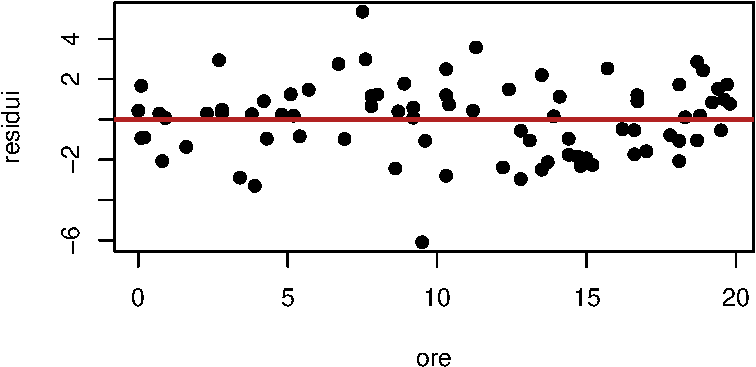
\includegraphics[width=0.55\linewidth,height=\textheight,keepaspectratio]{dispensa-statistica-descrittiva_files/figure-pdf/unnamed-chunk-156-1.pdf}
\end{center}

\subsubsection{Quando la relazione non è
lineare}\label{quando-la-relazione-non-uxe8-lineare}

\begin{center}
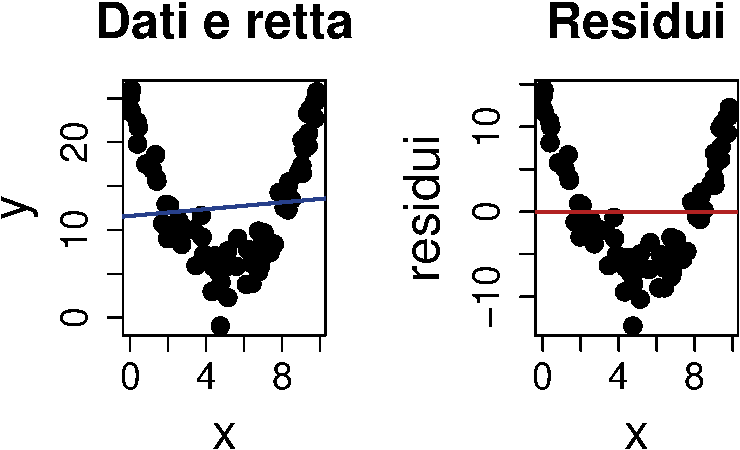
\includegraphics[width=0.9\linewidth,height=\textheight,keepaspectratio]{dispensa-statistica-descrittiva_files/figure-pdf/unnamed-chunk-158-1.pdf}
\end{center}

I residui hanno una chiara forma a ``U'': il modello lineare sovrastima
al centro e sottostima agli estremi \(\rightarrow\) l'assunto di
linearità è violato

\subsubsection{Istogramma dei residui}\label{istogramma-dei-residui}

\begin{Shaded}
\begin{Highlighting}[]
\FunctionTok{hist}\NormalTok{(studio}\SpecialCharTok{$}\NormalTok{residui, }\AttributeTok{freq =} \ConstantTok{FALSE}\NormalTok{, }\AttributeTok{xlab =} \StringTok{"residui"}\NormalTok{, }\AttributeTok{col =} \StringTok{"gray90"}\NormalTok{)}
\FunctionTok{curve}\NormalTok{(}\FunctionTok{dnorm}\NormalTok{(x, }\AttributeTok{mean =} \DecValTok{0}\NormalTok{, }\AttributeTok{sd =} \FunctionTok{sd}\NormalTok{(studio}\SpecialCharTok{$}\NormalTok{residui)), }
      \AttributeTok{add =} \ConstantTok{TRUE}\NormalTok{, }\AttributeTok{col =} \StringTok{"firebrick"}\NormalTok{, }\AttributeTok{lwd =} \DecValTok{2}\NormalTok{)}
\end{Highlighting}
\end{Shaded}

\begin{center}
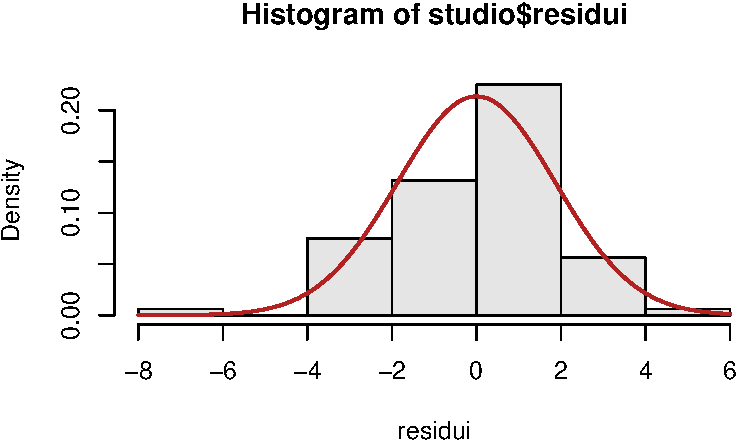
\includegraphics[width=0.55\linewidth,height=\textheight,keepaspectratio]{dispensa-statistica-descrittiva_files/figure-pdf/unnamed-chunk-159-1.pdf}
\end{center}

La linea rossa è la distribuzione normale con media 0 e sd pari a quella
dei residui

\subsubsection{Q-Q plot dei residui}\label{q-q-plot-dei-residui}

Confronta i quantili dei residui con quelli di una distribuzione
normale: se i residui sono normali, i punti stanno \textbf{sulla retta}

\begin{Shaded}
\begin{Highlighting}[]
\FunctionTok{qqnorm}\NormalTok{(studio}\SpecialCharTok{$}\NormalTok{residui, }\AttributeTok{pch =} \DecValTok{19}\NormalTok{)}
\FunctionTok{qqline}\NormalTok{(studio}\SpecialCharTok{$}\NormalTok{residui, }\AttributeTok{col =} \StringTok{"firebrick"}\NormalTok{, }\AttributeTok{lwd =} \DecValTok{2}\NormalTok{)}
\end{Highlighting}
\end{Shaded}

\begin{center}
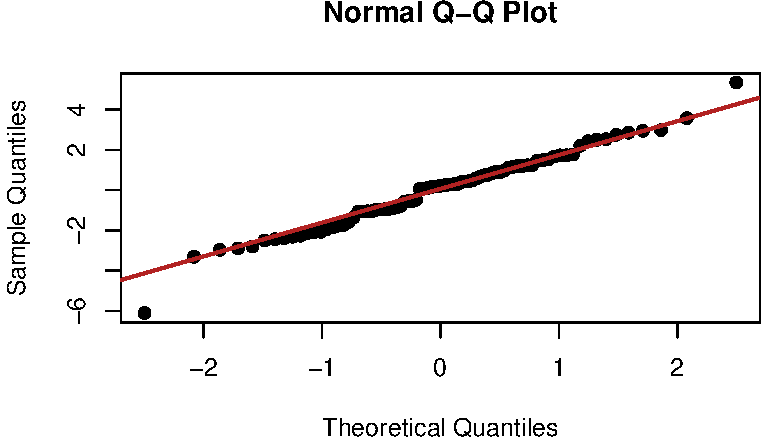
\includegraphics[width=0.5\linewidth,height=\textheight,keepaspectratio]{dispensa-statistica-descrittiva_files/figure-pdf/unnamed-chunk-160-1.pdf}
\end{center}

\subsubsection{Quando i residui non sono
normali}\label{quando-i-residui-non-sono-normali}

\begin{center}
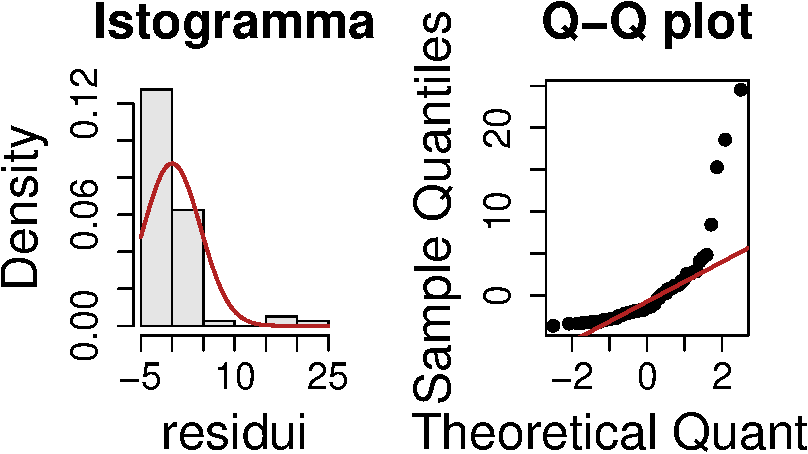
\includegraphics[width=0.8\linewidth,height=\textheight,keepaspectratio]{dispensa-statistica-descrittiva_files/figure-pdf/unnamed-chunk-162-1.pdf}
\end{center}

Distribuzione asimmetrica: coda lunga a destra, i punti si allontanano
dalla retta agli estremi

\subsubsection{Omoschedasticità}\label{omoschedasticituxe0}

La variabilità dei residui deve essere \textbf{costante} per tutti i
valori attesi: la ``nuvola'' deve avere la stessa ampiezza da sinistra a
destra

\begin{Shaded}
\begin{Highlighting}[]
\FunctionTok{plot}\NormalTok{(studio}\SpecialCharTok{$}\NormalTok{attesi, studio}\SpecialCharTok{$}\NormalTok{residui, }\AttributeTok{pch =} \DecValTok{19}\NormalTok{,}
     \AttributeTok{xlab =} \StringTok{"valori attesi"}\NormalTok{, }\AttributeTok{ylab =} \StringTok{"residui"}\NormalTok{)}
\FunctionTok{abline}\NormalTok{(}\AttributeTok{h =} \DecValTok{0}\NormalTok{, }\AttributeTok{col =} \StringTok{"firebrick"}\NormalTok{, }\AttributeTok{lwd =} \DecValTok{2}\NormalTok{)}
\end{Highlighting}
\end{Shaded}

\begin{center}
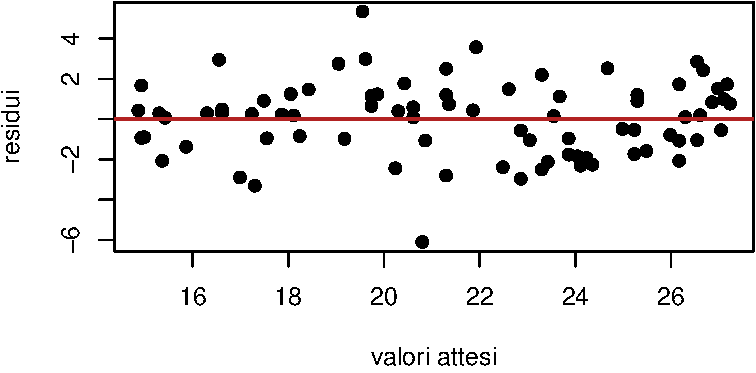
\includegraphics[width=0.55\linewidth,height=\textheight,keepaspectratio]{dispensa-statistica-descrittiva_files/figure-pdf/unnamed-chunk-163-1.pdf}
\end{center}

\begin{center}
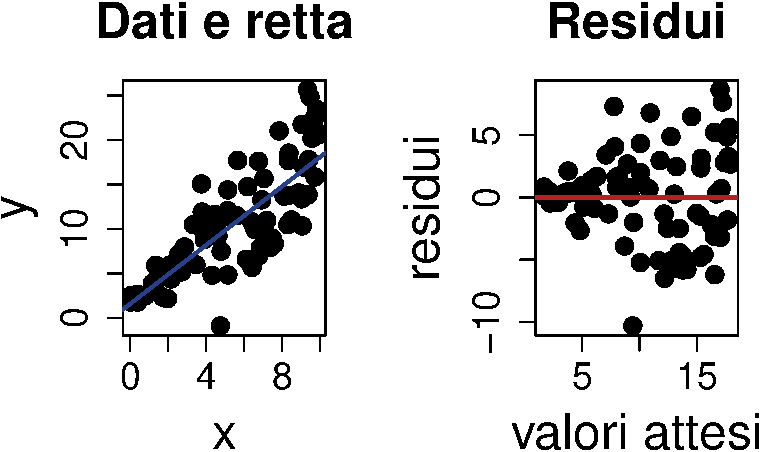
\includegraphics[width=0.8\linewidth,height=\textheight,keepaspectratio]{dispensa-statistica-descrittiva_files/figure-pdf/unnamed-chunk-165-1.pdf}
\end{center}

Forma ``a imbuto'': i residui sono sempre più dispersi al crescere dei
valori attesi \(\rightarrow\) eteroschedasticità

\subsubsection{Indipendenza delle
osservazioni}\label{indipendenza-delle-osservazioni}

Dipende soprattutto da \textbf{come sono stati raccolti i dati}: ogni
osservazione deve essere indipendente dalle altre

Esempi di violazione: misure ripetute sulla stessa persona, studenti
della stessa classe, dati raccolti nel tempo

Se i dati hanno un ordine (es. ordine di raccolta), si possono guardare
i residui in quell'ordine: non deve esserci nessun andamento

\begin{Shaded}
\begin{Highlighting}[]
\FunctionTok{plot}\NormalTok{(studio}\SpecialCharTok{$}\NormalTok{residui, }\AttributeTok{type =} \StringTok{"b"}\NormalTok{, }\AttributeTok{pch =} \DecValTok{19}\NormalTok{,}
     \AttributeTok{xlab =} \StringTok{"ordine di raccolta"}\NormalTok{, }\AttributeTok{ylab =} \StringTok{"residui"}\NormalTok{)}
\FunctionTok{abline}\NormalTok{(}\AttributeTok{h =} \DecValTok{0}\NormalTok{, }\AttributeTok{col =} \StringTok{"firebrick"}\NormalTok{, }\AttributeTok{lwd =} \DecValTok{2}\NormalTok{)}
\end{Highlighting}
\end{Shaded}

\begin{center}
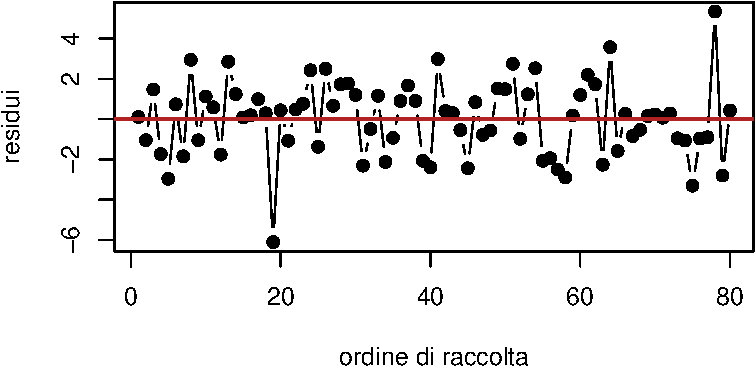
\includegraphics[width=0.45\linewidth,height=\textheight,keepaspectratio]{dispensa-statistica-descrittiva_files/figure-pdf/unnamed-chunk-166-1.pdf}
\end{center}

\subsubsection{Cosa guardare nei
residui}\label{cosa-guardare-nei-residui}

\begin{longtable}[]{@{}
  >{\raggedright\arraybackslash}p{(\linewidth - 4\tabcolsep) * \real{0.2308}}
  >{\raggedright\arraybackslash}p{(\linewidth - 4\tabcolsep) * \real{0.2308}}
  >{\raggedright\arraybackslash}p{(\linewidth - 4\tabcolsep) * \real{0.5385}}@{}}
\toprule\noalign{}
\begin{minipage}[b]{\linewidth}\raggedright
Assunto
\end{minipage} & \begin{minipage}[b]{\linewidth}\raggedright
Grafico
\end{minipage} & \begin{minipage}[b]{\linewidth}\raggedright
Cosa si deve vedere
\end{minipage} \\
\midrule\noalign{}
\endhead
\bottomrule\noalign{}
\endlastfoot
Linearità & \texttt{plot(x,\ residui)} & Nuvola casuale attorno a 0 \\
Normalità & \texttt{hist(residui)}, \texttt{qqnorm(residui)} & Forma a
campana, punti sulla retta \\
Omoschedasticità & \texttt{plot(attesi,\ residui)} & Ampiezza costante
(niente imbuti) \\
Indipendenza & \texttt{plot(residui,\ type\ =\ "b")} & Nessun andamento
nell'ordine \\
\end{longtable}

\vspace{3mm}

Tutto parte da due funzioni:

\begin{Shaded}
\begin{Highlighting}[]
\NormalTok{attesi }\OtherTok{\textless{}{-}} \FunctionTok{fitted}\NormalTok{(modello)}
\NormalTok{residui }\OtherTok{\textless{}{-}} \FunctionTok{residuals}\NormalTok{(modello)}
\end{Highlighting}
\end{Shaded}

\section{Materiale supplementare}\label{materiale-supplementare}

\subsection{Outliers e casi influenti}\label{outliers-e-casi-influenti}

\subsubsection{Definizioni}\label{definizioni}

\textbf{Outlier}: Il valore di un'osservazione nella variabile
dipendente è anomalo dato il valore del predittore (ha un residuo molto
grande)

\textbf{Leverage} (leva): Quanto il valore di un'osservazione nel
predittore è lontano dalla media del predittore \(\rightarrow\) quanto
\emph{potenzialmente} può spostare la retta

\textbf{Influential case}: Una singola osservazione che riesce a
spostare l'intera retta di regressione

\vspace{2mm}

Un'osservazione può essere:

\begin{itemize}
\item
  Un outlier (ma non un influential case)
\item
  Un punto ad alta leva in linea con gli altri (ma non un influential
  case)
\item
  Un outlier influente (anomalo \textbf{e} ad alta leva)
\end{itemize}

\subsubsection{Un outlier living the
life}\label{un-outlier-living-the-life}

\begin{center}
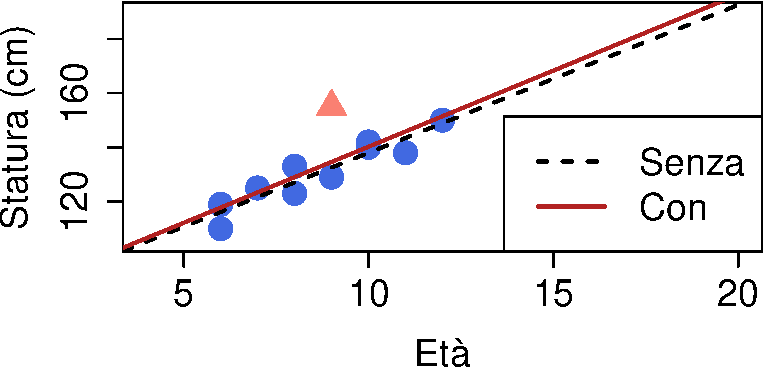
\includegraphics[width=0.75\linewidth,height=\textheight,keepaspectratio]{dispensa-statistica-descrittiva_files/figure-pdf/unnamed-chunk-169-1.pdf}
\end{center}

Il triangolo rosa è un outlier: è anomalo rispetto alla nuvola di punti,
ma essendo vicino alla media dell'età sposta la retta di poco
(soprattutto in alto, l'intercetta)

\subsubsection{Un punto ad alta leva living the
life}\label{un-punto-ad-alta-leva-living-the-life}

\begin{center}
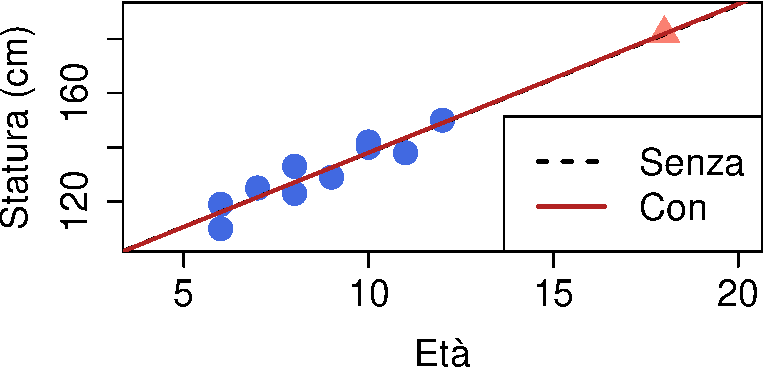
\includegraphics[width=0.75\linewidth,height=\textheight,keepaspectratio]{dispensa-statistica-descrittiva_files/figure-pdf/unnamed-chunk-170-1.pdf}
\end{center}

Il triangolo rosa è lontano dagli altri sull'asse delle \(x\) (alta
leva), ma è in linea con l'andamento dei dati: la retta non cambia

\subsubsection{Un outlier influential case living the
life}\label{un-outlier-influential-case-living-the-life}

\begin{center}
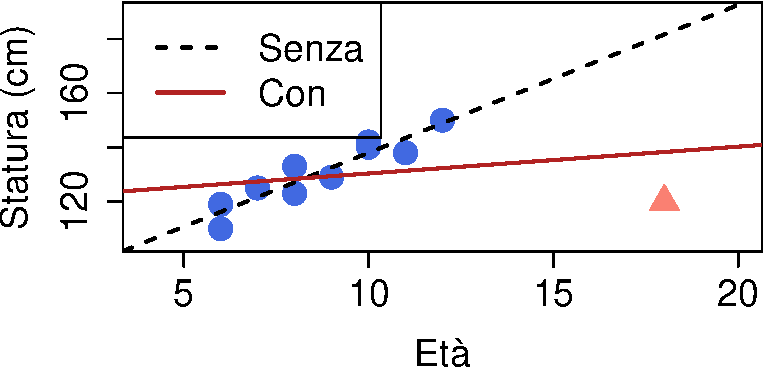
\includegraphics[width=0.75\linewidth,height=\textheight,keepaspectratio]{dispensa-statistica-descrittiva_files/figure-pdf/unnamed-chunk-171-1.pdf}
\end{center}

Il triangolo rosa è anomalo \textbf{e} lontano dagli altri sull'asse
delle \(x\): ne sposta drasticamente la pendenza

\subsection{Leverage e distanza di
Cook}\label{leverage-e-distanza-di-cook}

\subsubsection{Tirare fuori leverage e distanza di
Cook}\label{tirare-fuori-leverage-e-distanza-di-cook}

Come per i residui, anche gli indici di influenza si estraggono dal
modello e si guardano

\texttt{hatvalues()}: leverage di ogni osservazione

\texttt{cooks.distance()}: distanza di Cook \(\rightarrow\) quanto
cambiano \emph{tutti} i valori attesi se l'osservazione viene tolta
(combina residuo e leverage)

\begin{Shaded}
\begin{Highlighting}[]
\NormalTok{influente }\OtherTok{\textless{}{-}} \FunctionTok{rbind}\NormalTok{(dat, }\FunctionTok{c}\NormalTok{(}\AttributeTok{soggetto =} \DecValTok{11}\NormalTok{, }\AttributeTok{eta =} \DecValTok{18}\NormalTok{, }\AttributeTok{statura =} \DecValTok{120}\NormalTok{))}
\NormalTok{mod\_inf }\OtherTok{\textless{}{-}} \FunctionTok{lm}\NormalTok{(statura }\SpecialCharTok{\textasciitilde{}}\NormalTok{ eta, }\AttributeTok{data =}\NormalTok{ influente)}
\NormalTok{influente}\SpecialCharTok{$}\NormalTok{leva }\OtherTok{\textless{}{-}} \FunctionTok{hatvalues}\NormalTok{(mod\_inf)}
\NormalTok{influente}\SpecialCharTok{$}\NormalTok{cook }\OtherTok{\textless{}{-}} \FunctionTok{cooks.distance}\NormalTok{(mod\_inf)}
\end{Highlighting}
\end{Shaded}

\begin{Shaded}
\begin{Highlighting}[]
\FunctionTok{round}\NormalTok{(influente, }\DecValTok{2}\NormalTok{)}
\end{Highlighting}
\end{Shaded}

\begin{verbatim}
   soggetto eta statura leva cook
1         1   6     110 0.20 0.29
2         2   6     119 0.20 0.06
3         3   7     125 0.15 0.00
4         4   8     123 0.11 0.01
5         5   8     133 0.11 0.01
6         6   9     129 0.09 0.00
7         7  10     140 0.09 0.04
8         8  10     142 0.09 0.05
9         9  11     138 0.11 0.02
10       10  12     150 0.14 0.21
11       11  18     120 0.70 9.25
\end{verbatim}

\subsubsection{Il grafico della distanza di
Cook}\label{il-grafico-della-distanza-di-cook}

Una soglia spesso usata: \(D_i > 4/n\)

\begin{Shaded}
\begin{Highlighting}[]
\FunctionTok{plot}\NormalTok{(influente}\SpecialCharTok{$}\NormalTok{cook, }\AttributeTok{type =} \StringTok{"h"}\NormalTok{, }\AttributeTok{lwd =} \DecValTok{3}\NormalTok{,}
     \AttributeTok{xlab =} \StringTok{"osservazione"}\NormalTok{, }\AttributeTok{ylab =} \StringTok{"distanza di Cook"}\NormalTok{)}
\FunctionTok{abline}\NormalTok{(}\AttributeTok{h =} \DecValTok{4} \SpecialCharTok{/} \FunctionTok{nrow}\NormalTok{(influente), }\AttributeTok{col =} \StringTok{"firebrick"}\NormalTok{, }\AttributeTok{lty =} \DecValTok{2}\NormalTok{, }\AttributeTok{lwd =} \DecValTok{2}\NormalTok{)}
\end{Highlighting}
\end{Shaded}

\begin{center}
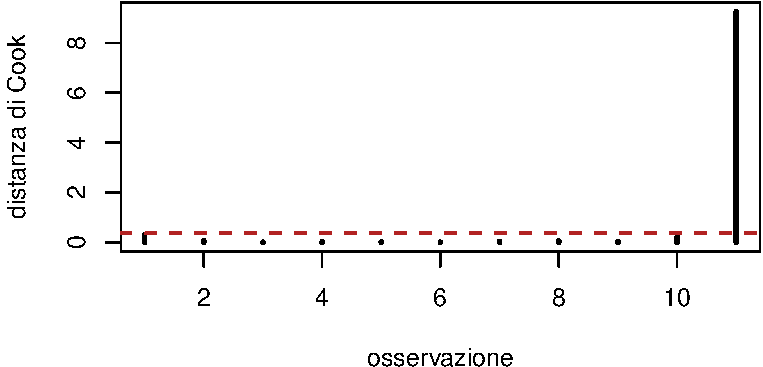
\includegraphics[width=0.5\linewidth,height=\textheight,keepaspectratio]{dispensa-statistica-descrittiva_files/figure-pdf/unnamed-chunk-174-1.pdf}
\end{center}

\begin{Shaded}
\begin{Highlighting}[]
\FunctionTok{which}\NormalTok{(influente}\SpecialCharTok{$}\NormalTok{cook }\SpecialCharTok{\textgreater{}} \DecValTok{4} \SpecialCharTok{/} \FunctionTok{nrow}\NormalTok{(influente))}
\end{Highlighting}
\end{Shaded}

\begin{verbatim}
[1] 11
\end{verbatim}

\chapter{Funzioni riassuntive dei
moduli}\label{funzioni-riassuntive-dei-moduli}

\section{Operatori}\label{operatori-1}

\subsection{Artitmetici}\label{artitmetici}

\begin{longtable}[]{@{}lll@{}}
\toprule\noalign{}
Simbolo & Significato & Note \\
\midrule\noalign{}
\endhead
\bottomrule\noalign{}
\endlastfoot
+ & Addizione & \\
- & Sottrazione & \\
* & Moltiplicazione & \\
/ & Divisione & \\
\^{} & Elevamento a potenza & \\
\end{longtable}

\subsection{Di confronto}\label{di-confronto}

\begin{longtable}[]{@{}lll@{}}
\toprule\noalign{}
Simbolo & Significato & Note \\
\midrule\noalign{}
\endhead
\bottomrule\noalign{}
\endlastfoot
\textless{} & Minore & \\
\textgreater{} & Maggiore & \\
\textless= & Minore uguale & \\
\textgreater= & Maggiore uguale & \\
== & Uguale & \\
!= & Diverso & \\
\end{longtable}

\subsection{Logici}\label{logici}

\begin{longtable}[]{@{}
  >{\raggedright\arraybackslash}p{(\linewidth - 4\tabcolsep) * \real{0.1800}}
  >{\raggedright\arraybackslash}p{(\linewidth - 4\tabcolsep) * \real{0.3800}}
  >{\raggedright\arraybackslash}p{(\linewidth - 4\tabcolsep) * \real{0.4400}}@{}}
\toprule\noalign{}
\begin{minipage}[b]{\linewidth}\raggedright
Simbolo
\end{minipage} & \begin{minipage}[b]{\linewidth}\raggedright
Significato
\end{minipage} & \begin{minipage}[b]{\linewidth}\raggedright
Note
\end{minipage} \\
\midrule\noalign{}
\endhead
\bottomrule\noalign{}
\endlastfoot
\& & Congiunzione & Intersezione tra insiemi \(\land\) (\(\cap\)) \\
\textbar{} & Disgiunzione & Unione tra insiemi \(\lor\) \(\cup\) \\
! & Negazione & \(\lnot\) \\
\&! & Disgiunzione esclusiva & \\
\%in\% & Incluzione & \\
\end{longtable}

\section{Valori di verità}\label{valori-di-verituxe0}

\begin{longtable}[]{@{}lll@{}}
\toprule\noalign{}
Valore & Significato & Note \\
\midrule\noalign{}
\endhead
\bottomrule\noalign{}
\endlastfoot
TRUE & Vero & Es. X\textgreater2 confronta ogni valore di X con 2 \\
FALSE & Falso & \\
\end{longtable}

\section{Operatori e funzioni utili}\label{operatori-e-funzioni-utili}

\begin{longtable}[]{@{}
  >{\raggedright\arraybackslash}p{(\linewidth - 4\tabcolsep) * \real{0.2222}}
  >{\raggedright\arraybackslash}p{(\linewidth - 4\tabcolsep) * \real{0.2889}}
  >{\raggedright\arraybackslash}p{(\linewidth - 4\tabcolsep) * \real{0.4889}}@{}}
\toprule\noalign{}
\begin{minipage}[b]{\linewidth}\raggedright
Funzione
\end{minipage} & \begin{minipage}[b]{\linewidth}\raggedright
Significato
\end{minipage} & \begin{minipage}[b]{\linewidth}\raggedright
Note
\end{minipage} \\
\midrule\noalign{}
\endhead
\bottomrule\noalign{}
\endlastfoot
\texttt{\textless{}-} & Operatore di assegnazione & Uguale a
\texttt{assign()} oppure \texttt{=} \\
\texttt{c(...)} & Concatenazione di valori & \texttt{c(1:n)} restituisce
valori da 1 a n con passo 1; \texttt{c(1,n)} restituisce solo 1 e n \\
\texttt{vettore{[}i{]}} & Operatore di selezione per i vettori, dove
\texttt{i} è l'indice della posizione a cui si vuole accedere & Es.
\texttt{A\textless{}-c(1,8,5,0)}; \texttt{A{[}c(1,4){]}} restituisce
valori in posizione 1 e 4 \\
\texttt{dati{[}i,\ j{]}} & Operatore di selezione per strutture di dati
(matrici, dataframe), dove \texttt{i} è l'indice della riga, \texttt{j}
della colonna & Es. \texttt{data{[}4,\ 12{]}} restituisce il valore
della cella che si trova all'incrocio tra la quarta riga e la dodicesima
colonna \\
\texttt{data\$variabile} & Visualizza la variabile richiamata & \\
\texttt{read.csv2("")} & Legge un file di dati esterno &
\texttt{sep\ =";",\ dec\ =",",\ header\ =\ TRUE"} \\
\end{longtable}

\section{Convertitori}\label{convertitori}

\begin{longtable}[]{@{}
  >{\raggedright\arraybackslash}p{(\linewidth - 4\tabcolsep) * \real{0.2222}}
  >{\raggedright\arraybackslash}p{(\linewidth - 4\tabcolsep) * \real{0.2889}}
  >{\raggedright\arraybackslash}p{(\linewidth - 4\tabcolsep) * \real{0.4889}}@{}}
\toprule\noalign{}
\begin{minipage}[b]{\linewidth}\raggedright
Funzione
\end{minipage} & \begin{minipage}[b]{\linewidth}\raggedright
Significato
\end{minipage} & \begin{minipage}[b]{\linewidth}\raggedright
Note
\end{minipage} \\
\midrule\noalign{}
\endhead
\bottomrule\noalign{}
\endlastfoot
\texttt{as.numeric(A)} & Converte in variabile numerica & \\
\texttt{as.factor(A)} & Converte in variabile categoriale/nominale &
Richiede variabile testuale \\
\texttt{factor(A,\ levels=c("a1",...,"ak"),\ ordered=TRUE)} & Converte
in variabile ordinale & Va inserito ordine dei livelli teorici \\
\texttt{as.matrix(data.frame)} & Converte un data.frame in oggetto
numerico & \\
\end{longtable}

\section{Strumenti}\label{strumenti}

\begin{longtable}[]{@{}lll@{}}
\toprule\noalign{}
Funzione & Significato & Note \\
\midrule\noalign{}
\endhead
\bottomrule\noalign{}
\endlastfoot
\texttt{remove(...)} & Rimuove valori assegnati & \\
\texttt{rm(...)} & Rimuove oggetti & \\
\texttt{rm(list=ls())} & Rimuove tutto ciò che è in memoria & \\
\texttt{ls()} & Visualizza oggetti in memoria & \\
\texttt{example(comando)} & Fornisce esempio d'uso & \\
\texttt{?comando} & Mostra guida & \\
\end{longtable}

\section{Funzioni matematiche}\label{funzioni-matematiche}

\begin{longtable}[]{@{}
  >{\raggedright\arraybackslash}p{(\linewidth - 4\tabcolsep) * \real{0.2222}}
  >{\raggedright\arraybackslash}p{(\linewidth - 4\tabcolsep) * \real{0.2889}}
  >{\raggedright\arraybackslash}p{(\linewidth - 4\tabcolsep) * \real{0.4889}}@{}}
\toprule\noalign{}
\begin{minipage}[b]{\linewidth}\raggedright
Funzione
\end{minipage} & \begin{minipage}[b]{\linewidth}\raggedright
Significato
\end{minipage} & \begin{minipage}[b]{\linewidth}\raggedright
Note
\end{minipage} \\
\midrule\noalign{}
\endhead
\bottomrule\noalign{}
\endlastfoot
\texttt{log(...)} & Logaritmo naturale & \\
\texttt{exp(...)} & Esponenziale & \\
\texttt{abs(...)} & Valore assoluto & \\
\texttt{sqrt(...)} & Radice quadrata & \\
\texttt{round(...)} & Arrotondamento & \\
\texttt{sign(...)} & Funzione segno & \\
\texttt{pi} & Costante pi greco & \\
\texttt{max(...)} & Valore massimo & \\
\texttt{min(...)} & Valore minimo & \\
\texttt{sum(...)} & Somma & \\
\texttt{mean(...)} & Media & \\
\texttt{mean(...,\ trim=n)} & Media troncata & Elimina outlier con
0\textless=n\textless=0.5 \\
\texttt{sd(...)} & Deviazione standard & \\
\texttt{var(...)} & Varianza & \\
\texttt{median(...)} & Mediana (2° quartile) & \\
\texttt{quantile(X,\ probs)} & Calcola quantile & \\
\texttt{IQR(...)} & Differenza interquartilica, \(Q_3-Q_1\) & \\
\texttt{range(...)} & Intervallo (min e max) & Identico a
\texttt{c(min(X),max(X))} \\
\texttt{rep(n,\ k)} & Replica \texttt{n} per \texttt{k} volte & \\
\texttt{dim(...)} & Dimensioni oggetto tabellare &
\texttt{dim(...){[}1{]}} righe, \texttt{dim(...){[}2{]}} colonne \\
\texttt{cumsum(...)} & Somma cumulata & \\
\texttt{length(...)} & Numero elementi di un vettore & \\
\texttt{which(...)} & Posizione di valori che soddisfano condizione &
Es. \texttt{which(x\textless{}3)} \\
\texttt{levels(...)} & Etichette assegnate a fattori & \\
\texttt{numeric(n)} & Vettore vuoto lunghezza n & \\
\texttt{rownames(...)} & Nomi righe & \\
\texttt{colnames(...)} & Nomi colonne & \\
\texttt{summary(...)} & Riassume contenuto & Anche modelli
\texttt{lm(...)} \\
\texttt{str(X)} & Controlla struttura oggetto & \\
\texttt{cov(X,Y)} & Covarianza campionaria & \\
\texttt{cor(X,Y)} & Correlazione lineare & \(-1\leq r \leq 1\) \\
\end{longtable}

\section{Matrici}\label{matrici-1}

\begin{longtable}[]{@{}
  >{\raggedright\arraybackslash}p{(\linewidth - 4\tabcolsep) * \real{0.2222}}
  >{\raggedright\arraybackslash}p{(\linewidth - 4\tabcolsep) * \real{0.2889}}
  >{\raggedright\arraybackslash}p{(\linewidth - 4\tabcolsep) * \real{0.4889}}@{}}
\toprule\noalign{}
\begin{minipage}[b]{\linewidth}\raggedright
Funzione
\end{minipage} & \begin{minipage}[b]{\linewidth}\raggedright
Significato
\end{minipage} & \begin{minipage}[b]{\linewidth}\raggedright
Note
\end{minipage} \\
\midrule\noalign{}
\endhead
\bottomrule\noalign{}
\endlastfoot
\texttt{matrix(y,\ r,\ c)} & Matrice \(r \times c\) con valori
\texttt{y} & Riempimento per colonne \\
\texttt{matrix(y,\ r,\ c,\ byrow=TRUE)} & Matrice & Riempimento per
righe \\
\texttt{t(M)} & Trasposta di M & \\
\texttt{*} & Prodotto tra matrici & \\
\end{longtable}

\section{Liste e Data Frame}\label{liste-e-data-frame}

\begin{longtable}[]{@{}
  >{\raggedright\arraybackslash}p{(\linewidth - 4\tabcolsep) * \real{0.2222}}
  >{\raggedright\arraybackslash}p{(\linewidth - 4\tabcolsep) * \real{0.2889}}
  >{\raggedright\arraybackslash}p{(\linewidth - 4\tabcolsep) * \real{0.4889}}@{}}
\toprule\noalign{}
\begin{minipage}[b]{\linewidth}\raggedright
Funzione
\end{minipage} & \begin{minipage}[b]{\linewidth}\raggedright
Significato
\end{minipage} & \begin{minipage}[b]{\linewidth}\raggedright
Note
\end{minipage} \\
\midrule\noalign{}
\endhead
\bottomrule\noalign{}
\endlastfoot
\texttt{list()} & Costruisce lista di oggetti & Prima creare oggetti,
poi richiamarli nella lista \\
\texttt{data.frame(...)} & Costruisce tabella di variabili & Variabili
devono avere stessa lunghezza \\
\texttt{apply(DATI,MARGIN,FUN)} & Applica funzione per righe
(\texttt{1})/colonne (\texttt{2}) & Es. \texttt{apply(DATI,1,sum)} \\
\texttt{cbind(...)} & Unisce colonne & Variabili devono avere stessa
lunghezza \\
\texttt{rbind(...)} & Unisce righe & \\
\texttt{head(df)} & Mostra prime 6 righe dataframe & \\
\texttt{tail(df)} & Mostra ultime 6 righe dataframe & \\
\end{longtable}

\section{Distribuzioni di frequenza}\label{distribuzioni-di-frequenza}

\begin{longtable}[]{@{}
  >{\raggedright\arraybackslash}p{(\linewidth - 4\tabcolsep) * \real{0.2222}}
  >{\raggedright\arraybackslash}p{(\linewidth - 4\tabcolsep) * \real{0.2889}}
  >{\raggedright\arraybackslash}p{(\linewidth - 4\tabcolsep) * \real{0.4889}}@{}}
\toprule\noalign{}
\begin{minipage}[b]{\linewidth}\raggedright
Funzione
\end{minipage} & \begin{minipage}[b]{\linewidth}\raggedright
Significato
\end{minipage} & \begin{minipage}[b]{\linewidth}\raggedright
Note
\end{minipage} \\
\midrule\noalign{}
\endhead
\bottomrule\noalign{}
\endlastfoot
\texttt{table(A)} & Tabella frequenze di variabile & \\
\texttt{table(A,B)} & Tabella di contingenza & \\
\texttt{margin.table(T,margin)} & Frequenze marginali & \texttt{1}
righe, \texttt{2} colonne \\
\texttt{T/sum(T)} & Frequenze relative & \\
\texttt{prop.table(T,margin)} & Probabilità condizionate & \\
\texttt{cumsum(table(X))} & Frequenze cumulate assolute & \\
\texttt{cumsum(table(X)/length(X))} & Frequenze cumulate relative & \\
\texttt{table(...)/length(...)} & Frequenze relative & \\
\end{longtable}

\section{Funzioni grafiche}\label{funzioni-grafiche}

\begin{longtable}[]{@{}
  >{\raggedright\arraybackslash}p{(\linewidth - 4\tabcolsep) * \real{0.2222}}
  >{\raggedright\arraybackslash}p{(\linewidth - 4\tabcolsep) * \real{0.2889}}
  >{\raggedright\arraybackslash}p{(\linewidth - 4\tabcolsep) * \real{0.4889}}@{}}
\toprule\noalign{}
\begin{minipage}[b]{\linewidth}\raggedright
Funzione
\end{minipage} & \begin{minipage}[b]{\linewidth}\raggedright
Significato
\end{minipage} & \begin{minipage}[b]{\linewidth}\raggedright
Note
\end{minipage} \\
\midrule\noalign{}
\endhead
\bottomrule\noalign{}
\endlastfoot
\texttt{hist(X,breaks)} & Istogramma & \texttt{breaks=} Calcolo ampiezza
bin \\
\texttt{boxplot(X)} & Boxplot & anche
\texttt{boxplot(X,Y,names=c("X","Y"))} \\
\texttt{runif(N,0,1)} & \texttt{N} valori casuali presi da distribuzione
uniforme & tra 0 e 1 \\
\texttt{density(X,bw)} & Stima densità & Usare
\texttt{plot(density(...))} \\
\texttt{par(mfrow=c(n1,n2))} & Imposta finestra grafica multipla &
\texttt{n1}=righe, \texttt{n2}=colonne \\
\texttt{skew(...)} & Misura asimmetria & \\
\texttt{kurt(...)} & Misura curtosi & \\
\texttt{plot(X,Y)} & Grafico di dispersione & \\
\end{longtable}

\section{Associazione variabili
categoriali}\label{associazione-variabili-categoriali}

\begin{longtable}[]{@{}lll@{}}
\toprule\noalign{}
Funzione & Significato & Note \\
\midrule\noalign{}
\endhead
\bottomrule\noalign{}
\endlastfoot
\texttt{chisq.test(T)\$statistic} & Calcola chi-quadrato osservato & \\
\texttt{chisq.test(T)\$expected} & Calcola frequenze teoriche & \\
\end{longtable}

\section{Regressione lineare}\label{regressione-lineare-1}

\begin{longtable}[]{@{}
  >{\raggedright\arraybackslash}p{(\linewidth - 4\tabcolsep) * \real{0.2222}}
  >{\raggedright\arraybackslash}p{(\linewidth - 4\tabcolsep) * \real{0.2889}}
  >{\raggedright\arraybackslash}p{(\linewidth - 4\tabcolsep) * \real{0.4889}}@{}}
\toprule\noalign{}
\begin{minipage}[b]{\linewidth}\raggedright
Funzione
\end{minipage} & \begin{minipage}[b]{\linewidth}\raggedright
Significato
\end{minipage} & \begin{minipage}[b]{\linewidth}\raggedright
Note
\end{minipage} \\
\midrule\noalign{}
\endhead
\bottomrule\noalign{}
\endlastfoot
\texttt{lm(Y\textasciitilde{}X)} & Modello regressione lineare & Y
dipendente, X indipendente \\
\texttt{abline(retta,...)} & Traccia retta sul grafico &
\texttt{abline(lm(Y\textasciitilde{}X))} \\
\texttt{cor(X,Y)\^{}2} & Bontà di adattamento (R\^{}2) & \\
\texttt{retta\$residuals} & Residui modello & Es.
\texttt{plot(X,E);\ abline(0,0)} \\
\end{longtable}




\end{document}
